\documentclass[9pt, addpoints]{exam}

\usepackage[spanish]{babel}
\usepackage[utf8]{inputenc}
\usepackage[dvips]{graphicx}
\usepackage{amsmath}
\usepackage{amsfonts}
\usepackage{amssymb}
\usepackage{mathtools}
\usepackage{pifont}
\usepackage{multicol}
%\usepackage{psfrag}
\usepackage{color}
\usepackage{latexsym}
\usepackage{epsfig}
%\usepackage{pstricks}
%\usepackage[T1]{fontenc}

\usepackage{tikz,pgfplots}
\usepgfplotslibrary{fillbetween}

% Language selection 
\newif\ifspanish
\spanishtrue % For the spanish version
%\spanishfalse % For the english version

% Opción para las soluciones
\printanswers

\def\dunodcero{\begin{array}{c} D=1 \\ \gtrless \\ D=0 \end{array}}
\def\dceroduno{\begin{array}{c} D=0 \\ \gtrless \\ D=1 \end{array}}
\newcommand{\pfa}{P_{\text{FA}}} 
\newcommand{\pmis}{P_{\text{M}}} 
\newcommand{\pdet}{P_{\text{D}}} 
\newcommand{\perr}{P_{\text{e}}}

\ifspanish
\newcommand{\ej}{Ejercicio }
\else
\newcommand{\ej}{Exercise }
\fi

\hyphenation{im-pres-cin-di-ble}

\setlength{\textheight}{23cm} \setlength{\textwidth}{15cm}
\setlength{\marginparsep}{2mm} \setlength{\marginparwidth}{2cm}

\spanishdecimal{.}
\pointsinmargin
\marginpointname{\%}
\pagestyle{head}

%%%%%%%%%%
\ifspanish
\header{Teoría de la Decisión}{Problemas}{Curso Académico 2019/2020}
\else
\header{Decision Theory}{Problems}{Academic Year 2019/2020}
\fi

\headrule


\begin{document}

\ifspanish

\begin{center}
  ~~\\
  {\center{\bf \LARGE Teoría de la Decisión: Problemas}} \\ ~~\\  ~~\\
  \fbox{\fbox{\parbox{6in}{
  Los problemas y ejercicios que se incluyen pertenecen en su mayoría a exámenes de asignaturas relacionadas con la Teoría de la Decisión. Los números entre paréntesis indican los temas tratados por cada problema, entre los siguientes:
  \begin{itemize}
  \item[2.1.] Decisión multiclase.
  \item[2.2.] Decisión binaria.
  \item[2.3.] Caso binario con verosimilitudes gaussianas.
  \item[2.4.] Caracterización de clasificadores mediante la curva ROC.
  \item[2.5.] Otras reglas de clasificación: Neyman-Pearson y minimax.
  \item[2.6.] Función discriminante.
   \end{itemize}
  }}}
\end{center}
\begin{center}
  \fbox{\fbox{\parbox{6in}{\centering Notación: \begin{itemize}
 \item Decisor ML: Decisor de máxima verosimilitud [$\phi_{\rm ML}(\mathbf x)$].
  \item Decisor MAP: Decisor máximo a posteriori [$\phi_{\rm MAP}(\mathbf x)$].
  \item LRT: Test de razón de verosimilitudes.
  \item $P_{\rm e}$: probabilidad de error.  
  \item $P_{\rm FA}$: probabilidad de falsa alarma. 
  \item $P_{\rm M}$: probabilidad de pérdidas. 
  \item $P_{\rm D}$: probabilidad de detección. 
  \item Curva ROC: curva característica de operación.
   \end{itemize}
  }}}
\end{center}

\else

\begin{center}
  ~~\\
  {\center{\bf \LARGE Detection Theory: Problems}} \\ ~~\\  ~~\\
  \fbox{\fbox{\parbox{6in}{
  Most of the problems and exercises of this collection have been taken from previous years exams on subjects related to Decision Theory. The topics covered by each exercise are shown next to the exercise number according to:
  \begin{itemize}
  \item[2.1.] Multiclass classification.
  \item[2.2.] Binary decision.
  \item[2.3.] Binary decision with Gaussian likelihoods.
  \item[2.4.] Characterization of classifiers using ROC curves.
  \item[2.5.] Other classification rules: Neyman-Pearson and minimax.
  \item[2.6.] Discriminant functions.
   \end{itemize}
  }}}
\end{center}
\begin{center}
  \fbox{\fbox{\parbox{6in}{\centering Notation: \begin{itemize}
 \item ML decider: Maximum likelihood decider [$\phi_{\rm ML}(\mathbf x)$].
  \item MAP decider: Maximum {\em a posteriori} decider [$\phi_{\rm MAP}(\mathbf x)$].
  \item LRT: Likelihood ratio test.
  \item $P_{\rm e}$: Probability of error.  
  \item $P_{\rm FA}$: Probability of false alarm. 
  \item $P_{\rm M}$: Probability of missing. 
  \item $P_{\rm D}$: Probability of detection. 
  \item ROC curve: Operating characteristic curve.
   \end{itemize}
  }}}
\end{center}

\fi

%%%%%%%%%%%%%%%%%
\begin{questions}

%%%%%%%%%%%%%%%%%%%%%%%%%
\section{Decision Theory}

%%%%%%%%%%%%%%%%%%%%%%%%%%%%%%%%%%%%%%%%%%%%%%%%%%%%%%%%%%%%%%%%%%%
%  Examen TDS Enero 2010 (convocatoria extraordinaria) P1
\qformat{\textbf{\ej \thequestion ~~ (2.2; 2.4; 2.6)} ~~ \linefill}
\ifspanish

\question En un problema de clasificación binaria se sabe que las observaciones presentan las siguientes distribuciones:
 $$					  \begin{array}{ll}
					  p_{X|H}(x|0) = \exp (-x), & \quad	x>0 \\
					  p_{X|H}(x|1) =  a \exp (-a x), & \quad	x>0\\				
					  \end{array}	  $$
con $a >1$. Para la toma de la decisión se dispone de un conjunto de $K$ observaciones independientes tomadas bajo la misma hipótesis:  $\left\lbrace X^{(k)} \right\rbrace_{k=1}^K$.
\begin{parts}
\part Obténgase el decisor ML basado en el conjunto de observaciones  $\left\lbrace X^{(k)} \right\rbrace_{k=1}^K$ y compruébese, a partir de resultado obtenido, que $T=\sum_{k=1}^K X^{(k)} $ es un estadístico suficiente para la decisión.
Considérese para el resto del ejercicio $K=2$. 
\part Calcúlense las verosimilitudes del estadístico $T$, $p_{T|H}(t|0)$ y $p_{T|H}(t|1)$.
\part Calcúlense, en función del valor de $\eta$, las $P_{\rm FA}$ y $P_{\rm M}$ del decisor de umbral
$$ t \dceroduno \eta$$
\part Represéntese de forma aproximada la curva ROC del decisor anterior, indicando:
\begin{itemize}
\item Cómo se desplaza el punto de trabajo al aumentar $\eta$.
\item Cómo se modificaría la curva ROC si creciese el número de observaciones disponibles ($K$).
\item Cómo se modificaría la curva ROC al incrementar el valor de $a$.
\end{itemize}

\end{parts}

\begin{solution}
\begin{parts}
\part $t \dceroduno \displaystyle \frac{K \ln a}{a-1}$ \\
\part $  \begin{array}{ll}
					  p_{T|H}(t|0) = t\exp (-t), & \quad	t>0 \\
					  p_{T|H}(t|1) =  a^2 t \exp (-at), & \quad	t>0\\				
					  \end{array}	  $
\part $P_{\rm FA} = 1- (\eta +1) \exp(-\eta)  \quad P_{\rm M} = (a\eta +1) \exp(-a\eta)$ 
\part 
\begin{itemize}
\item Para $\eta = 0, \; P_{\rm FA} = P_{\rm D} = 0$; Para $\eta \rightarrow \infty, \; P_{\rm FA} = P_{\rm D} = 1$.
\item Si crece el número de observaciones, necesariamente debe mejorar la curva ROC.
\item Si crece el valor de $a$, también debe mejorar la curva ROC. Una comprobación rigurosa sería:
$\displaystyle \frac{\partial P_{\rm M}}{\partial a}=-a \eta^2 exp(- a \eta ) < 0$, luego la probabilidad de pérdida decrece al aumentar el valor de $a$.
\end{itemize}
\end{parts}
\end{solution}

\else

\question Consider a binary classification problem where observations are distributed according to:
 $$					  \begin{array}{ll}
					  p_{X|H}(x|0) = \exp (-x), & \quad	x>0 \\
					  p_{X|H}(x|1) =  a \exp (-a x), & \quad	x>0\\				
					  \end{array}	  $$
with $a >1$. For the decision, $K$ independent observations, taken under the same hypothesis, are available: $\left\lbrace X^{(k)} \right\rbrace_{k=1}^K$.
\begin{parts}
\part Obtain the ML classifier based on the set of observations $\left\lbrace X^{(k)} \right\rbrace_{k=1}^K$ and check, using such a classifier, that $T=\sum_{k=1}^K X^{(k)}$ is a sufficient statistic for the decision.
\end{parts}
Consider $K=2$ for the rest of the exercise. 
\begin{parts}
\setcounter{partno}{1}
\part Find the likelihoods in terms of the sufficient statistic $T$, $p_{T|H}(t|0)$ and $p_{T|H}(t|1)$.
\part Calculate $P_{\rm FA}$ and $P_{\rm M}$ for the following threshold decision maker, as a function of $\eta$:
$$ t \dceroduno \eta$$
\part Provide an approximate plot of the ROC curve for the previous decision maker, indicating:
\begin{itemize}
\item How the operation point moves when increasing $\eta$.
\item How the ROC curve would change if we had access to a larger number of observations $K$.
\item How the ROC curve changes as the value of $a$ increases.
\end{itemize}

\end{parts}

\begin{solution}
\begin{parts}
\part $t \dceroduno \displaystyle \frac{K \ln a}{a-1}$ \\
\part $  \begin{array}{ll}
					  p_{T|H}(t|0) = t\exp (-t), & \quad	t>0 \\
					  p_{T|H}(t|1) =  a^2 t \exp (-at), & \quad	t>0\\				
					  \end{array}	  $
\part $P_{\rm FA} = 1- (\eta +1) \exp(-\eta)  \quad P_{\rm M} = (a\eta +1) \exp(-a\eta)$ 
\part 
\begin{itemize}
\item For $\eta = 0, \; P_{\rm FA} = P_{\rm D} = 0$; for $\eta \rightarrow \infty, \; P_{\rm FA} = P_{\rm D} = 1$.
\item If the number of observations increases, then necessarily the performance of the classifier should improve (the area below the ROC curve increases).
\item The same occurs if the value of $a$ is increased.  A rigorous demonstration would be:
$\displaystyle \frac{\partial P_{\rm M}}{\partial a}=-a \eta^2 exp(- a \eta ) < 0$, thus $P_M$ decreases as the value of $a$ is increased.
\end{itemize}
\end{parts}

\end{solution}

\fi

%%%%%%%%%%%%%%%%%%%%%%%%%%%%%%%%%%%%%%%%%%%%%%%%%%%%%%%%%%%%%%%%%%%
%  Examen TDS Septiembre 2009 P1
\qformat{\textbf{\ej \thequestion ~~ (2.3; 2.6)} ~~ \linefill}
\ifspanish

\question  Considérese un sistema de comunicaciones en el que los símbolos ``$+1$'' ó ``$-1$'' se transmiten simultáneamente por dos canales ruidosos, tal y como se ilustra en la figura:
\begin{figure}[h]
\begin{center}
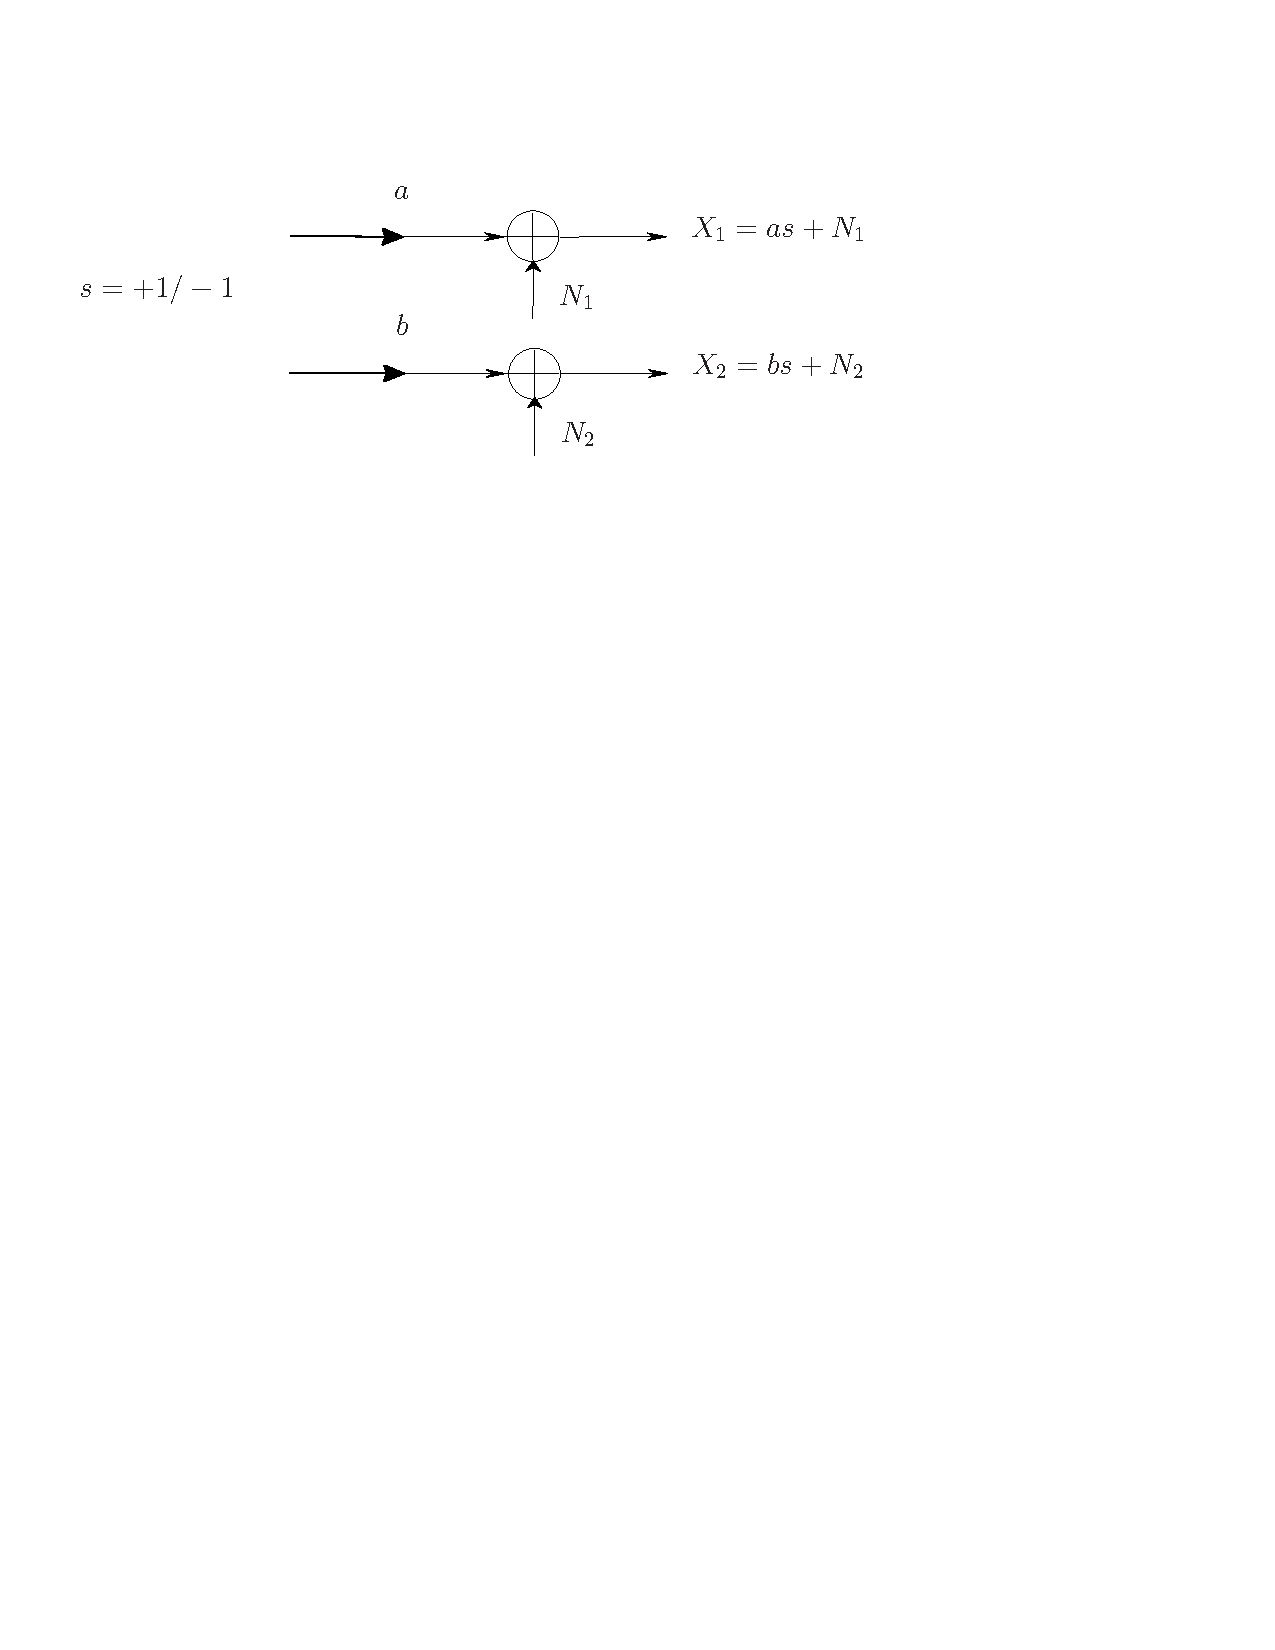
\includegraphics[width=12cm, trim=0cm 20.5cm 4cm 2.5cm]{Figuras/canal_gauss}
\end{center}
\end{figure}

siendo $a$ y $b$ dos constantes positivas desconocidas que caracterizan a los canales y $N_1$ y $N_2$ dos variables de ruido gaussiano caracterizados por
$$ \left( \begin{array}{c}  N_1 \\ N_2 \end{array}  \right) \sim G \left[ \left( \begin{array}{c}  0 \\ 0 \end{array}  \right), \left( \begin{array}{cc}  1 & \rho \\ \rho & 1 \end{array}  \right) \right].  $$
donde $|\rho|<1$. Se sabe, además, que las probabilidades de transmisión de ambos símbolos son iguales.
\begin{parts}
\part Si se desea construir un decisor para discriminar cuál fue el símbolo transmitido utilizando únicamente una de las dos observaciones disponibles, $X_1$ o $X_2$, indíquese cuál de las dos variables utilizaría, justificando su respuesta en función de los valores de las constantes.  Proporciónese la forma analítica del decisor ML correspondiente.
\part Obténgase el decisor binario de mínima probabilidad de error basado en la observación conjunta de $X_1$ y $X_2$, expresando el resultado como función de $a$, $b$ y $\rho$.  Simplifique la expresión de dicho decisor tanto como le sea posible.
\part Para $\rho = 0$, calcúlese la probabilidad de error del decisor dise\~{n}ado en b).  Exprese su resultado utilizando la función:
$$F(x) = 1- Q(x) = \int_{-\infty}^x \frac{1}{\sqrt{2\pi}} \exp{\left( - \frac{t^2}{2}\right) } \; dt$$

\end{parts}

\begin{solution}

\begin{parts}
\part $ \mbox{Si} \; a>b:  \quad  x_1 \dunodcero 0 \quad \quad  \quad  \quad \quad   \mbox{Si} \;  a<b: \quad  x_2 \dunodcero 0$
\part $(a - \rho b)x_1 + (b - \rho a)x_2 \dunodcero 0$
\part $\displaystyle  P_{\rm e}=F(-\sqrt{a^2+b^2})$ 
\end{parts}
 \end{solution}

\else

\question Consider a communication system in which one  of the symbols, ``$+1$'' or ``$-1$'', is simultaneously transmitted through two noisy channels, as illustrated in the figure:
\begin{figure}[h]
\begin{center}
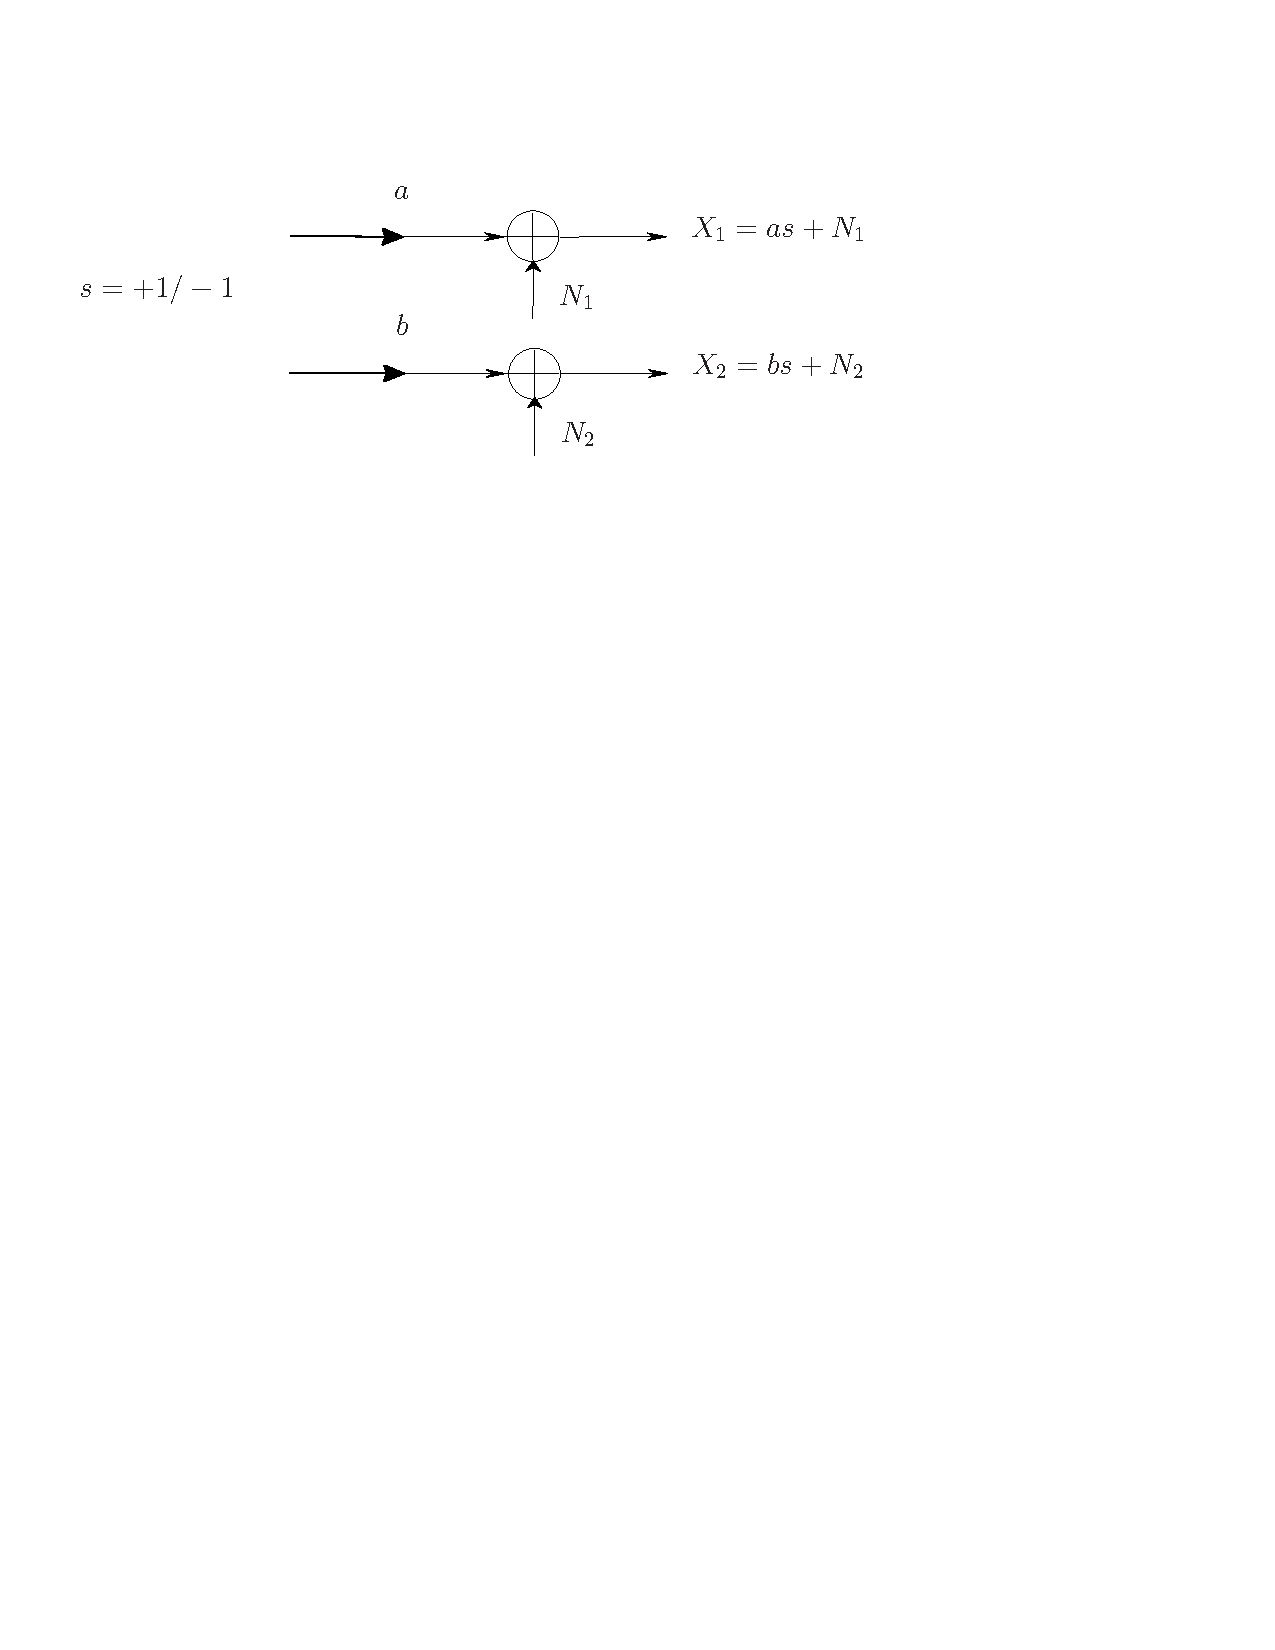
\includegraphics[width=12cm, trim=0cm 20.5cm 4cm 2.5cm]{Figuras/canal_gauss}
\end{center}
\end{figure}

with $a$ and $b$ being two unknown positive constants which characterize the channels, and where $N_1$ and $N_2$ are two Gaussian noises with joint pdf
$$ \left( \begin{array}{c}  N_1 \\ N_2 \end{array}  \right) \sim G \left[ \left( \begin{array}{c}  0 \\ 0 \end{array}  \right), \left( \begin{array}{cc}  1 & \rho \\ \rho & 1 \end{array}  \right) \right].  $$
It is also known that both symbols can be transmitted with equal {\em a priori} probabilities.
\begin{parts}
\part If we wish to design a decider for discriminating the transmitted symbol using just one of the two available observations, $X_1$ or $X_2$, indicate which of the two variables you would use, justifying your answer as a function of the values of constants $a$ and $b$.  Provide the analytical expression for the corresponding ML decider.
\part Obtain now the binary classifier with a minimum probability of error, based on the joint observation of $X_1$ and $X_2$, expressing it as a function of $a$, $b$, and $\rho$. Simplify your expression as much as possible.
\part For $\rho = 0$, calculate the probability of error of the decider obtained in b). Express your result by means of function:
$$F(x) = 1- Q(x) = \int_{-\infty}^x \frac{1}{\sqrt{2\pi}} \exp{\left( - \frac{t^2}{2}\right) } \; dt$$

\end{parts}

\begin{solution}

\begin{parts}
\part $ \mbox{If} \; a>b:  \quad  x_1 \dunodcero 0 \quad \quad  \quad  \quad \quad   \mbox{If} \;  a<b: \quad  x_2 \dunodcero 0$
\part $(a - \rho b)x_1 + (b - \rho a)x_2 \dunodcero 0$
\part $ P_{\rm e}=F\left(-\displaystyle\sqrt{a^2 + b^2}\right)$ 
\end{parts}

\end{solution}

\fi
 
%%%%%%%%%%%%%%%%%%%%%%%%%%%%%%%%%%%%%%%%%%%%%%%%%%%%%%%%%%%%%%%%%%%
%  Examen TDI Septiembre 2009 T1
\qformat{\textbf{\ej \thequestion ~~ (2.2; 2.4)} ~~ \linefill}
\ifspanish

\question Las siguientes verosimilitudes caracterizan un problema de decisión binario bidimensional con  $P_H(0)=3/5$:
\begin{align*}
p_{X_1,X_2|H}(x_1,x_2|0) &= 2,                      & 0<x_1<1, \quad 0<x_2<1-x_1  \\
p_{X_1,X_2|H}(x_1,x_2|1) &= 3\left( x_1+x_2\right), & 0<x_1<1, \quad 0<x_2<1-x_1 
\end{align*}

  
\begin{figure}[h]
\begin{center}
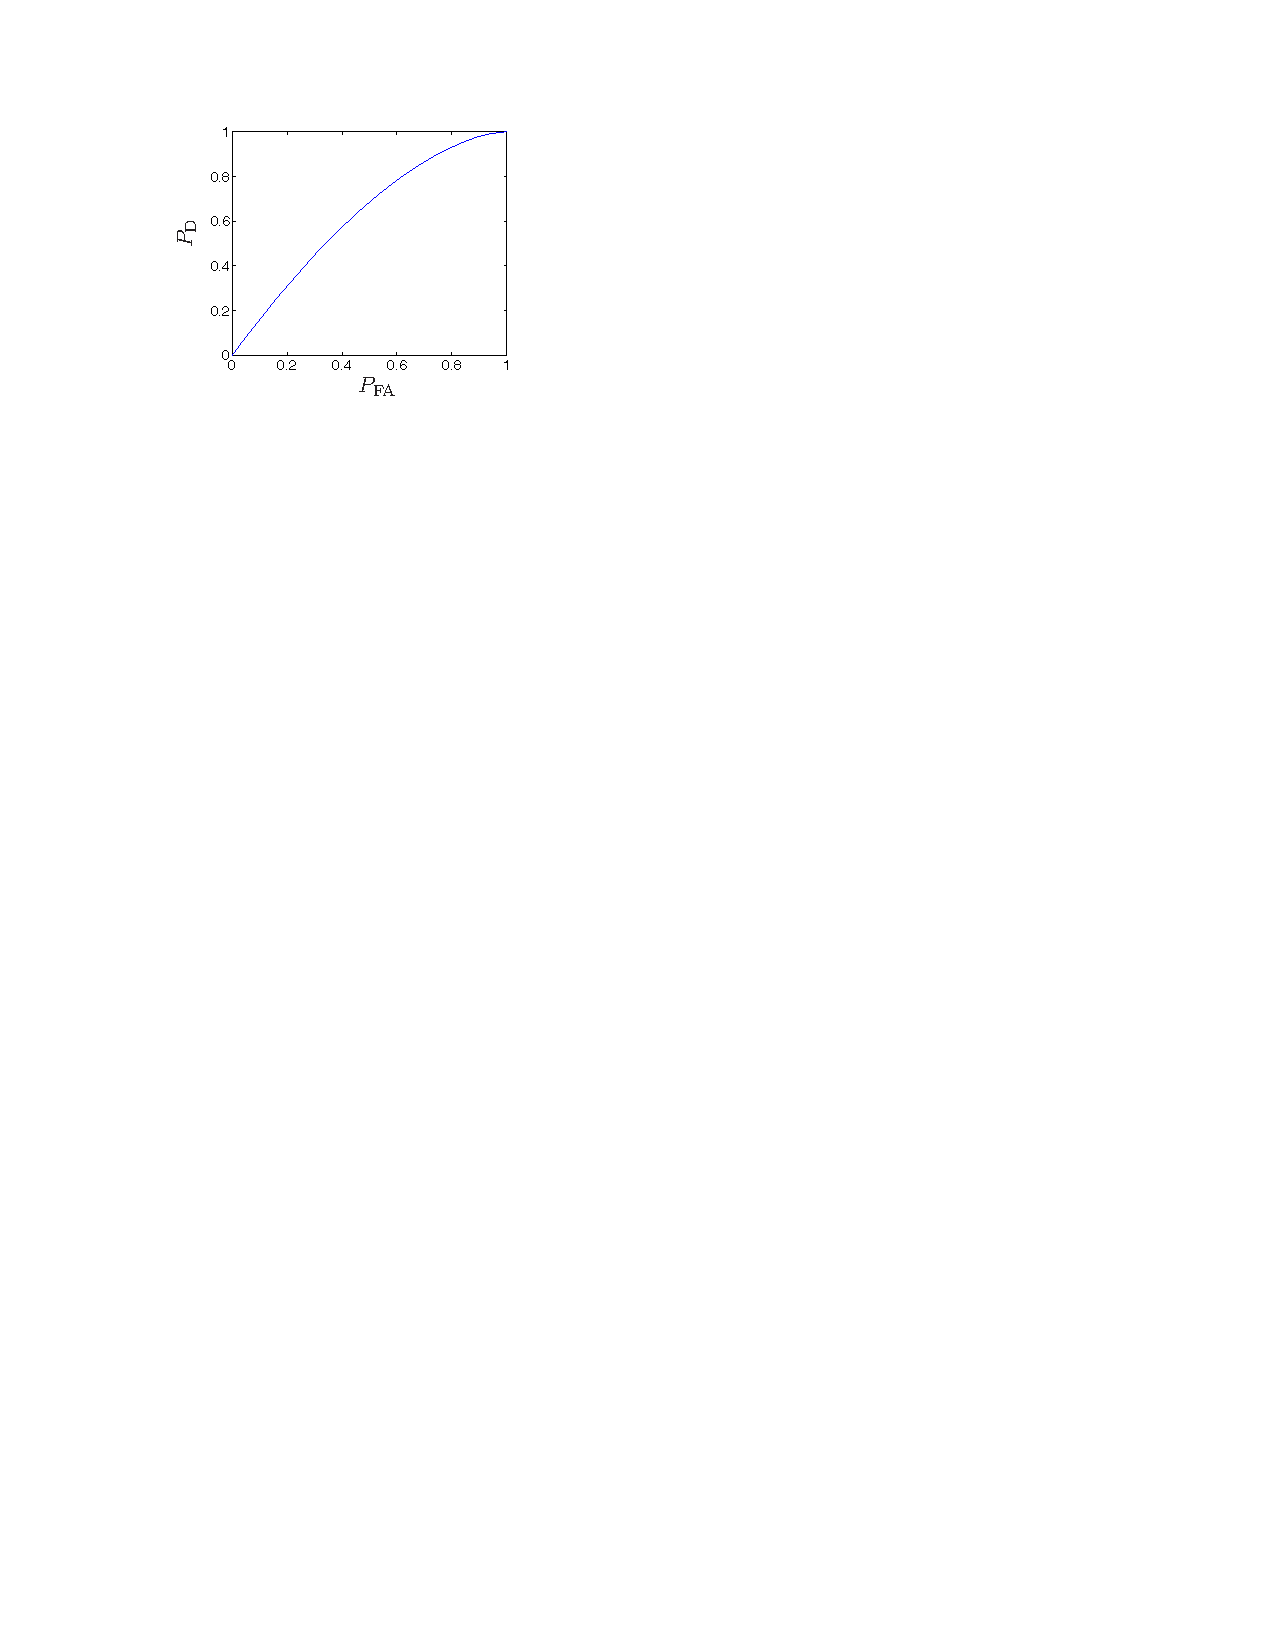
\includegraphics[width=14cm, trim=0cm 22cm 7cm 2cm]{Figuras/ROC}
\end{center}
\end{figure}

Considérese un decisor LRT genérico con umbral $\eta$,
\begin{parts}
\part Calcúlese la $P_{\rm FA}$ en función de $\eta$.
\part La siguiente figura representa la ROC {del LRT}.  Justificando su respuesta:
\begin{itemize}
\item {Indique} sobre la {ROC} cómo varía el punto de trabajo del decisor al aumentar o disminuir el umbral del test.
\item {Situe} sobre la {ROC} los puntos de trabajo correspondientes al decisor ML, al decisor de mínima probabilidad de error y al decisor de Neyman-Pearson con $P_{\rm FA} = 0.3$.
\end{itemize}

\end{parts}

\begin{solution}
\begin{parts}
\part $x_1+x_2 \dunodcero \dfrac{2}{3}\eta =\eta'  \quad \quad P_{\rm FA}=1-\eta'^2$
\part \begin{itemize}
\item $P_{\rm FA}$ y $P_{\rm D}$  decrecen al aumentar el umbral
\item
 	Decisor ML: $\eta=1$, $\eta'=\dfrac{2}{3}$, $P_{\rm FA}=\dfrac{5}{9}$.\\
	Decisor MAP: $\eta=\dfrac{3}{2}$,	$\eta'=1$,	$P_{\rm FA}=0$.\\
	Decisor N-P:	$P_{\rm FA}=0.3$.
	\end{itemize}
\end{parts}
\end{solution}

\else

\question The following likelihoods characterize a bidimensional binary decision problem with $P_H(0)=3/5$:
\begin{align*}
p_{X_1,X_2|H}(x_1,x_2|0) &= 2,                      & 0<x_1<1, \quad 0<x_2<1-x_1  \\
p_{X_1,X_2|H}(x_1,x_2|1) &= 3\left( x_1+x_2\right), & 0<x_1<1, \quad 0<x_2<1-x_1 
\end{align*}
 
\begin{figure}[h]
\begin{center}
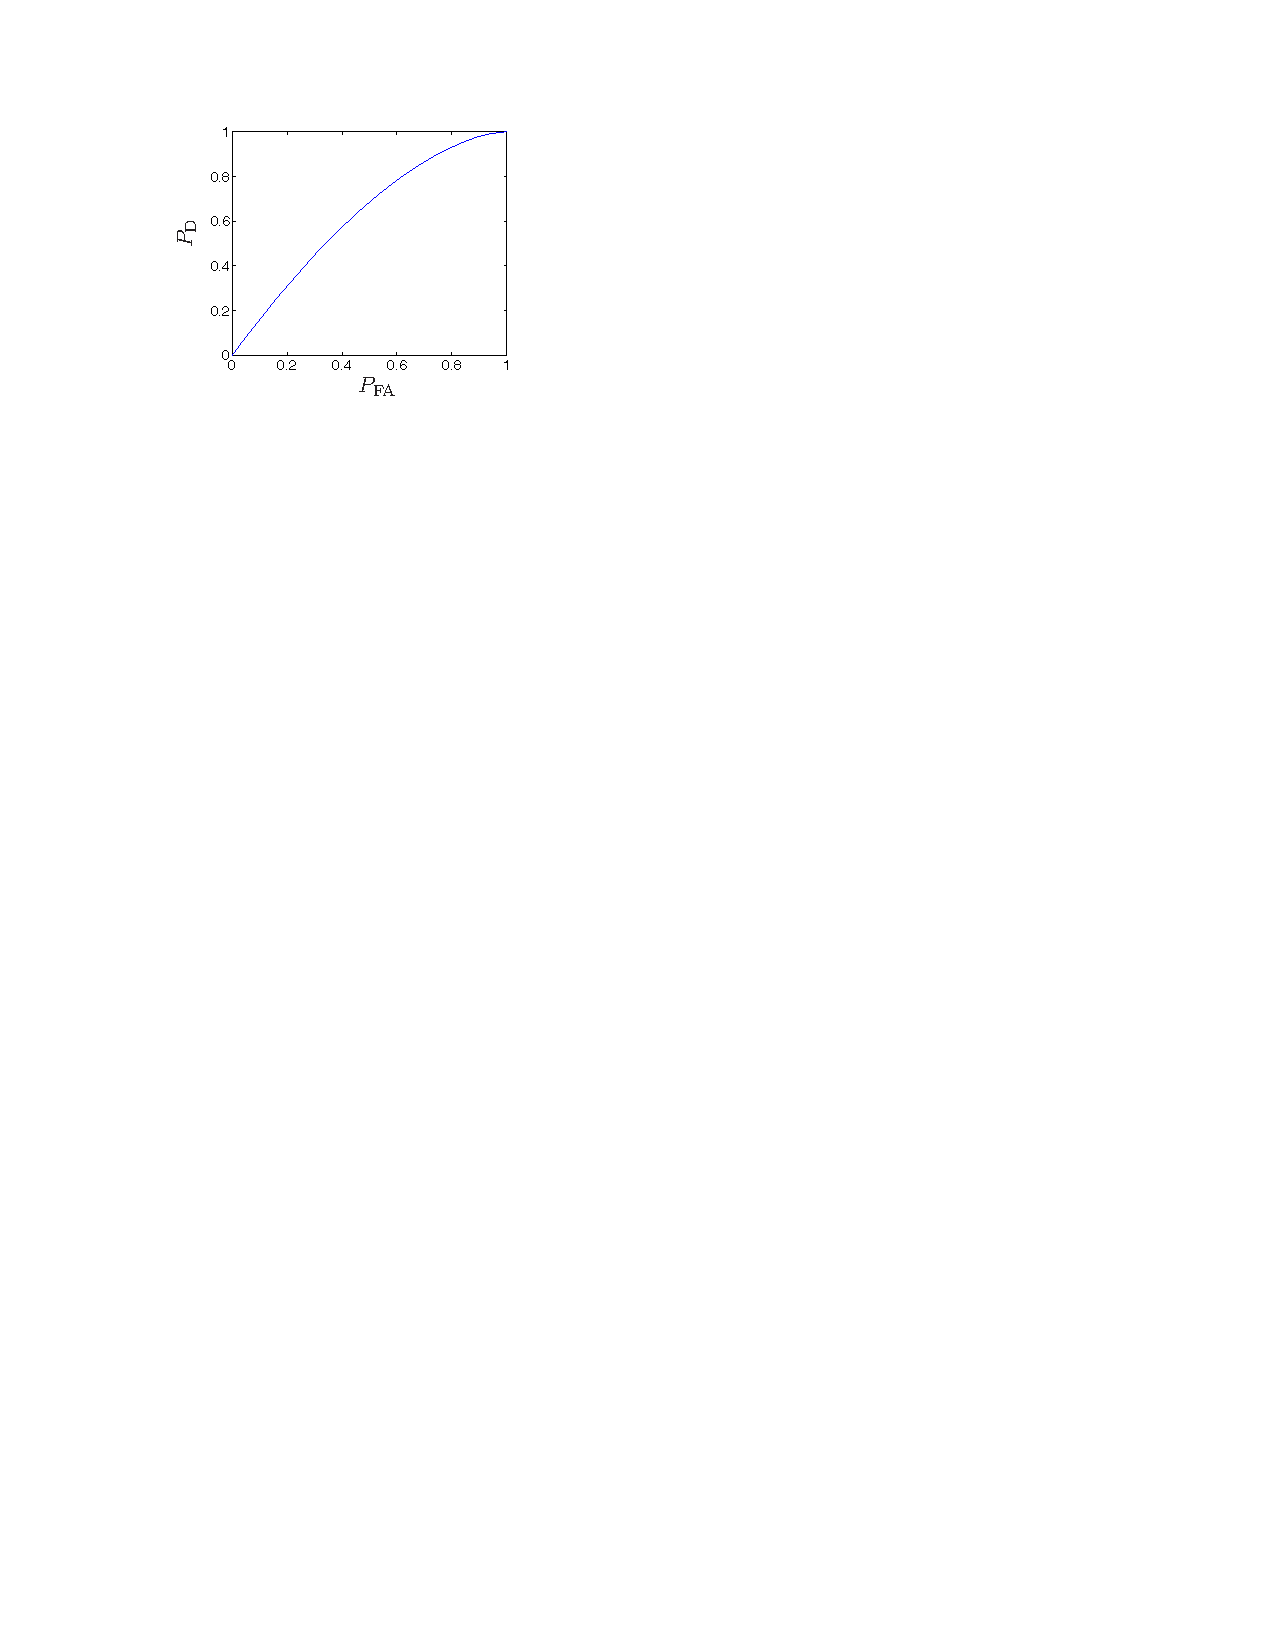
\includegraphics[width=14.5cm, trim=0cm 21.5cm 7cm 2cm]{Figuras/ROC}
\end{center}
\end{figure}

Consider a generic LRT decision maker with threshold $\eta$,
\begin{parts}
\part Calculate $P_{\rm FA}$ as a function of $\eta$.
\part The figure represents the ROC curve of the LRT. Justifying your answer:
\begin{itemize}
\item Indicate on the ROC how the operation point moves on the curve when increasing or decreasing the threshold of the test.
\item Place on the ROC the operation points corresponding to the ML classifier, to the decision maker with minimum probability of error, and to the Neyman-Pearson detector with $P_{\rm FA} = 0.3$.
\end{itemize}
\end{parts}

\begin{solution}
\begin{parts}
\part $x_1+x_2 \dunodcero \dfrac{2}{3}\eta =\eta'  \quad \quad P_{\rm FA}=1-\eta'^2$
\part \begin{itemize}
\item $P_{\rm FA}$ and $P_{\rm D}$ decrease as the threshold is increased.
\item
ML classifier: $\eta=1$, $\eta'=\dfrac{2}{3}$, $P_{\rm FA}=\dfrac{5}{9}$.\\
MAP classifier: $\eta=\dfrac{3}{2}$,	$\eta'=1$,	$P_{\rm FA}=0$.\\
N-P decision maker:	$P_{\rm FA}=0.3$.
	\end{itemize}
\end{parts}

\end{solution}

\fi

%%%%%%%%%%%%%%%%%%%%%%%%%%%%%%%%%%%%%%%%%%%%%%%%%%%%%%%%%%%%%%%%%%%
%  Examen TDI/TDS Junio 2009 T1
\qformat{\textbf{\ej \thequestion ~~ (2.3)} ~~ \linefill}
\ifspanish

\question {Considere} el par de hipótesis equiprobables:
$$ \begin{array}{ll} 
					  H=0:  & X = N \\
					  H=1:  & X = N + a S				  
					   \end{array}$$
donde $N$ y $S$ son variables aleatorias gaussianas independientes, con medias nulas y varianzas $v_n$ y $v_s$, respectivamente, y $a$ es una constante conocida.
\begin{parts}
\part {Verifique} que el test de mínima probabilidad de error tiene la forma
$$c_1 \exp \left( c_2x^2 \right) \gtrless \eta$$
y {calcule} las constantes $c_1$ y $c_2$, indicando el criterio de decisión asociado.
\part {Determine} las regiones de decisión sobre $x$. Nótese que dichas regiones pueden expresarse en función de las constantes $c_1$ y $c_2$.
\end{parts}

\begin{solution}
\begin{parts}
\part $c_1 \exp \left( c_2x^2 \right) \dunodcero 1$, donde $ \;  c_1 = \displaystyle   \frac{P_H(0)}{P_H(1)} \sqrt{\displaystyle  \frac{v_n}{v_n+a^2v_s}} \;$ y $\; c_2  = \displaystyle  \frac{1}{2v_n}-\displaystyle  \frac{1}{2\left( v_n+a^2v_s\right) }$
\part $ |x| \dunodcero \sqrt{\displaystyle  \frac{-\ln {c_1}}{c_2}} $
\end{parts}	 
\end{solution}

\else

\question Consider two equally probable hypotheses, with associated observations:
$$ \begin{array}{ll} 
					  H=0:  & X = N \\
					  H=1:  & X = N + a S				  
					   \end{array}$$
where $N$ and $S$ are independent Gaussian random variables, with zero mean and variances $v_n$ and $v_s$, respectively, and where $a$ is a known positive constant.
\begin{parts}
\part Verify that the minimum probability error test can be written down as
$$c_1 \exp \left( c_2x^2 \right) \gtrless \eta$$
and calculate the value of constants $c_1$ and $c_2$, indicating the associated criterion for the decision.
\part Determine the decision regions (over $x$) induced by the classifier. Note that such regions can be expressed as a function of constants $c_1$ and $c_2$.
\end{parts}

\begin{solution}
\begin{parts}
\part $c_1 \exp \left( c_2x^2 \right) \dunodcero 1$, where $ \;  c_1 = \displaystyle   \frac{P_H(0)}{P_H(1)} \sqrt{\displaystyle  \frac{v_n}{v_n+a^2v_s}} \;$ and $\; c_2  = \displaystyle  \frac{1}{2v_n}-\displaystyle  \frac{1}{2\left( v_n+a^2v_s\right) }$
\part $ |x| \dunodcero \sqrt{\displaystyle  \frac{-\ln {c_1}}{c_2}} $
\end{parts}	 
\end{solution}

\fi

%%%%%%%%%%%%%%%%%%%%%%%%%%%%%%%%%%%%%%%%%%%%%%%%%%%%%%%%%%%%%%%%%%%
% Examen TDI/TDS Junio 2009 P1 
\qformat{\textbf{\ej \thequestion ~~ (2.2)} ~~ \linefill}
\question 


\ifspanish

La densidad de probabilidad conjunta de las variables aleatorias $X$ y $Z$ es
 $$p_{X,Z}(x, z) = x + z, \quad \quad 0 \leq x \leq 1, \qquad 0 \leq z \leq 1$$
Considere el problema de decisión basado en la observación de $X$ (pero no de $Z$) dado por las hipótesis:
$$ \begin{array}{ll} 
		H=0:  & Z < 0.6\\
		H=1:  & Z > 0.6				  
   \end{array}$$
\begin{parts}
\part Determine $p_{Z|X}(z|x)$.
\part Obtenga las probabilidades a posteriori de ambas hipótesis.
\part Determinese el decisor MAP basado en $X$.
\part Aplicando el Teorema de Bayes, calcule $p_{X|H}(x|0)$ y $p_{X|H}(x|1)$.
\part Calcule la probabilidad de falsa alarma del decisor MAP.
\part Determine el decisor ML basado en $X$. 
\end{parts}

\begin{solution}

\begin{parts}
\part Sabiendo que
\begin{align*}
p_{X}(x)
	&= \int_{-\infty}^{\infty} p_{Z,X}(z,x) dz
	 = \int_0^1 (x+z) dz
	 = \frac{(x+1)^2}{2} - \frac{x^2}{2} \\
	&= x + \frac12,    \qquad 0 \le x \le 1
\end{align*}
resulta
\begin{align*}
p_{Z|X}(z|x)
	&= \frac{p_{Z,X}(z,x)}{p_X(x)}
	 = \frac{2 \left(x+z \right)}{2x+1},   \qquad 0 \le x \le 1, \quad  0 \le z \leq 1
\end{align*}

\part
\begin{align*}
P_{H|X}(0|x) 
	&= P\{H=0 |x\} 
	 = P\{Z < 0.6 | x\} 
	 = \int_{-\infty}^{0.6} p_{Z|X}(z|x) dz  \\
	&= \int_0^{0.6} \frac{2 \left(x+z \right)}{2x+1} dz 
	 = \frac{1.2x+0.36}{2x+1}   \\
P_{H|X}(1|x)
    &= 1 - P_{H|X}(0|x) = \frac{0.8 x + 0.64}{2x+1}
\end{align*}

\part El decisor MAP está dado por
\begin{align*}
P_{H|X}(1|x) \dunodcero \frac12 
	&\quad \Leftrightarrow \quad \frac{0.8 x + 0.64}{2x+1} \dunodcero \frac12   \\
	&\quad \Leftrightarrow \quad 0.8 x + 0.64 \dunodcero x + 0.5   \\
    &\quad \Leftrightarrow \quad x \dceroduno 0.7
\end{align*}

\part
Sabiendo que
\begin{align*}
P_H(0) &= \int_{-\infty}^\infty P_{H|X}(0|x) p_X(x) dx 
        = \int_0^1 \frac{1.2x+0.36}{2x+1} \left(x + \frac12\right) dx  \\
       &= \int_0^1 (0.6 x + 0.18) dx 
        = \frac12 \left( (0.6 + 0.18)^2 - 0.18^2  \right) = 0.48   \\
P_H(1) &= 1-P_H(0) = 0.52
\end{align*}
resulta
\begin{align*}
p_{X|H}(x|0) 
	&= \frac{P_{H|X}(0|x) p_X(x)}{P_H(0)}
	 = \frac{1}{0.48} \frac{1.2x+0.36}{2x+1} \left(x + \frac12\right) \\
    &= \frac{10 x+ 3}8 
\end{align*}
\begin{align*}
p_{X|H}(x|1)
	&= \frac{P_{H|X}(1|x) p_X(x)}{P_H(1)}
	 = \frac{1}{0.52} \frac{0.8 x + 0.64}{2x+1} \left(x + \frac12\right) \\
    &= \frac{10 x + 8}{13} 
\end{align*}
\part 
\begin{align*}
P_{\rm FA} 
	&= P\{D=1|H=0\} 
	 = P\{X < 0.7| H=0\} 
	 = \int_{-\infty}^{0.7} p_{X|H}(x|0) dx   \\
	&= \frac18 \int_0^{0.7} (10 x+ 3) dx 
     = 0.5687
\end{align*}
\part El decisor ML será
\begin{align*}
p_{X|H}(x|1) \dunodcero p_{X|H}(x|0)
	&\quad \Leftrightarrow \quad \frac{10 x + 8}{13} \dunodcero \frac{10 x+ 3}8    \\
    &\quad \Leftrightarrow \quad x \dceroduno 0.5
\end{align*}
\end{parts}
\end{solution}


\else


The joint probability density function of random variables $X$ and $Z$ is given by
 $$p_{X,Z}(x, z) = x + z, \quad \quad 0 \leq x \leq 1, \qquad 0 \leq z \leq 1$$
Consider the decision problem based on the observation of $X$ (but not $Z$), with hypotheses:
$$ \begin{array}{ll} 
	H=0:  & Z \le 0.6\\
	H=1:  & Z > 0.6				  
	\end{array}$$
\begin{parts}
\part Find $p_{Z|X}(z|x)$.
\part Obtain the {\em a posteriori} probabilities of both hypotheses.
\part Find the MAP classifier based on $X$.
\part Applying Bayes' Theorem, find the likelihoods $p_{X|H}(x|0)$ and $p_{X|H}(x|1)$.
\part Calculate the probability of false alarm of the MAP classifier.
\part Determine the ML classifier based on the observation of $X$. 
\end{parts}

\begin{solution}

\begin{parts}
\part Knowing that
\begin{align*}
p_{X}(x)
	&= \int_{-\infty}^{\infty} p_{Z,X}(z,x) dz
	 = \int_0^1 (x+z) dz
	 = \frac{(x+1)^2}{2} - \frac{x^2}{2} \\
	&= x + \frac12,    \qquad 0 \le x \le 1
\end{align*}
we obtain
\begin{align*}
p_{Z|X}(z|x)
	&= \frac{p_{Z,X}(z,x)}{p_X(x)}
	 = \frac{2 \left(x+z \right)}{2x+1},   \qquad 0 \le x \le 1, \quad  0 \le z \leq 1
\end{align*}

\part
\begin{align*}
P_{H|X}(0|x) 
	&= P\{H=0 |x\} 
	 = P\{Z < 0.6 | x\} 
	 = \int_{-\infty}^{0.6} p_{Z|X}(z|x) dz  \\
	&= \int_0^{0.6} \frac{2 \left(x+z \right)}{2x+1} dz 
	 = \frac{1.2x+0.36}{2x+1}   \\
P_{H|X}(1|x)
    &= 1 - P_{H|X}(0|x) = \frac{0.8 x + 0.64}{2x+1}
\end{align*}

\part The MAP decision-maker is given by
\begin{align*}
P_{H|X}(1|x) \dunodcero \frac12 
	&\quad \Leftrightarrow \quad \frac{0.8 x + 0.64}{2x+1} \dunodcero \frac12   \\
	&\quad \Leftrightarrow \quad 0.8 x + 0.64 \dunodcero x + 0.5   \\
    &\quad \Leftrightarrow \quad x \dceroduno 0.7
\end{align*}

\part
Knowing that
\begin{align*}
P_H(0) &= \int_{-\infty}^\infty P_{H|X}(0|x) p_X(x) dx 
        = \int_0^1 \frac{1.2x+0.36}{2x+1} \left(x + \frac12\right) dx  \\
       &= \int_0^1 (0.6 x + 0.18) dx 
        = \frac12 \left( (0.6 + 0.18)^2 - 0.18^2  \right) = 0.48   \\
P_H(1) &= 1-P_H(0) = 0.52
\end{align*}
we have
\begin{align*}
p_{X|H}(x|0) 
	&= \frac{P_{H|X}(0|x) p_X(x)}{P_H(0)}
	 = \frac{1}{0.48} \frac{1.2x+0.36}{2x+1} \left(x + \frac12\right) \\
    &= \frac{10 x+ 3}8 
\end{align*}
\begin{align*}
p_{X|H}(x|1)
	&= \frac{P_{H|X}(1|x) p_X(x)}{P_H(1)}
	 = \frac{1}{0.52} \frac{0.8 x + 0.64}{2x+1} \left(x + \frac12\right) \\
    &= \frac{10 x + 8}{13} 
\end{align*}
\part 
\begin{align*}
P_{\rm FA} 
	&= P\{D=1|H=0\} 
	 = P\{X < 0.7| H=0\} 
	 = \int_{-\infty}^{0.7} p_{X|H}(x|0) dx   \\
	&= \frac18 \int_0^{0.7} (10 x+ 3) dx 
     = 0.5687
\end{align*}
\part The ML decision-maker is
\begin{align*}
p_{X|H}(x|1) \dunodcero p_{X|H}(x|0)
	&\quad \Leftrightarrow \quad \frac{10 x + 8}{13} \dunodcero \frac{10 x+ 3}8    \\
    &\quad \Leftrightarrow \quad x \dceroduno 0.5
\end{align*}
\end{parts}
\end{solution}

\fi

%%%%%%%%%%%%%%%%%%%%%%%%%%%%%%%%%%%%%%%%%%%%%%%%%%%%%%%%%%%%%%%%%%%
% Examen TDI  Mayo 2009  (convocatoria extraordinaria) P1
\qformat{\textbf{\ej \thequestion ~~ (2.2;  2.4; 2.5)} ~~ \linefill}
\ifspanish

\question Considere el problema de decisión binario dado por $P_H(1) = 2 P_H(0)$ y verosimilitudes:
$$
\begin{array}{ll} 
	p_{X|H}(x | 0) = 2(1- x),  & 0 \leq x \leq 1  \\
	p_{X|H}(x | 1) = 2 x - 1,  & \dfrac{1}{2} \leq x \leq  \dfrac{3}{2}		  
\end{array}
$$
\begin{parts}
\part Determine el decisor bayesiano para los costes $c_{00} = c_{11} = 0$, $c_{10} = 4 c_{01}$.
\part Determine el decisor de Neyman-Pearson dado por $P_{\rm FA} \le 0.04$.
\part Determine, en función del parámetro $\alpha$, las probabilidades de detección y falsa alarma de la familia de decisores de la forma 
	 $$x \dunodcero \alpha$$
\part Represente gráficamente (de forma aproximada) la curva característica de operación (ROC), tomando $\alpha$ como parámetro libre, e indicando cómo varía el punto de trabajo del decisor en función de su valor.
\part Indique si los decisores de los apartados (a) y (b) se corresponden con algún punto de la ROC y, en su caso, indique con cuál(es).

\end{parts}

\begin{solution}

\begin{parts}
\part El decisor bayesiano para los costes dados esta dado por la regla de decisión:
\begin{align*}
(c_{01} &- c_{11}) P_H(1) p_{X|H}(x|1) \dunodcero (c_{10} - c_{00}) P_H(0) p_{X|H}(x|0) \\
	& \Leftrightarrow \quad c_{01} 2 P_H(0) p_{X|H}(x|1) \dunodcero 4 c_{01} P_H(0) p_{X|H}(x|0) \\
	& \Leftrightarrow \quad p_{X|H}(x|1) \dunodcero 2 p_{X|H}(x|0) \\
	& \Leftrightarrow \quad 
	      \left[\begin{array}{ll}
		        D = 0,                   & \text{if } 0 \le x \le \frac12 \\
		        2 x-1 \dunodcero 4(1-x), & \text{if } \frac12 \le x \le 1 \\
		        D = 1,                   & \text{if } 1 \le x \le \frac32
		        \end{array}
		  \right.   \\
	& \Leftrightarrow \quad 
	      \left[\begin{array}{ll}
		            D = 0,                 & \text{if } 0 \le x \le \frac12 \\
		            x \dunodcero \frac56,  & \text{if } \frac12 \le x \le 1 \\
		            D = 1,                 & \text{if } \frac32 \le x \le 1  
		         \end{array}
		  \right.   \\
	& \Leftrightarrow \quad 
	      x \dunodcero \frac56
\end{align*}
\part El LRT para umbral $\lambda \ge 0$ tiene la forma
\begin{align*}
p_{X|H}(x|1) \dunodcero \lambda p_{X|H}(x|0)
  & \Leftrightarrow \quad 
	  \left[\begin{array}{ll}
            D = 0,                          & \text{if } 0 \le x \le \frac12 \\
		    2x-1 \dunodcero 2\lambda (1-x), & \text{if } \frac12 \le x \le 1 \\
		    D = 1,                          & \text{if } 1 \le x \le \frac32
		    \end{array}
	  \right.   \\
  & \Leftrightarrow \quad 
      \left[\begin{array}{ll}
  	      D = 0,                                        & \text{if } 0 \le x \le \frac12 \\
  	      x \dunodcero \frac{2\lambda+1}{2(1+\lambda)}, & \text{if } \frac12 \le x \le 1 \\
  	      D = 1,                                        & \text{if } 1 \le x \le \frac32
  	      \end{array}
  	  \right.   \\
  & \Leftrightarrow \quad x \dunodcero \alpha
\end{align*}
donde $\alpha = \frac{2 \lambda + 1}{2(1+\lambda)} \in [\frac12, 1]$.

La probabilidad de falsa alarma será
\begin{align*}
P_{\rm FA} &= P_{D|H}(1|0) 
            = P\{x \ge \alpha | H=0\} \\
           &= \int_\alpha^\infty p_{X|H}(x|0) dx 
            = \int_\alpha^1 2(1-x) dx \\
           &= (1-\alpha)^2
\end{align*}
Tomando $P_{\rm FA}\le 0.04$, resulta $(1-\mu)^2 = 0.04$, luego $\mu=0.8$ y el decisor NP es
\begin{align*}
x \dunodcero 0.8
\end{align*}

\part De acuerdo con lo visto en el apartado (b), la probabilidad de falsa alarma, para cualquier $\alpha \in [0, \frac32]$ será:
\begin{align*}
P_{\rm FA} 
  &= \left[\begin{array}{ll} 
	       (1-\alpha)^2  & \quad 0 < \alpha < 1         \\
	       0             & \quad 1 < \alpha < \frac32
  	       \end{array}  
  	 \right.  
\end{align*}
Análogamente, la probabilidad de detección será
\begin{align*}
P_{\rm D} 
	&= P_{D|H}(1|1) 
     = P\{x \le \alpha | H=1 \}              
     = \int_\alpha^\infty p_{X|H}(x|1) dx  \\
    &= \left[\begin{array}{ll} 
			 1                              & \quad 0 < \alpha < \frac12 \\	  
			 \int_\alpha^\frac32 (2x-1) dx  & \quad \frac12 < \alpha < \frac32
  			 \end{array}  
	   \right.  	 \\
    &= \left[\begin{array}{ll} 
			 1                                  & \quad 0 < \alpha < \frac12	\\	  
			 1 - \left(\alpha-\frac12\right)^2  & \quad \frac12 < \alpha < \frac32   
  			 \end{array}  
	   \right.  	
\end{align*}

\part Basta con obtener algunos puntos significativos, y dibujar la ROC de forma aproximada. Por ejemplo:
\begin{align*}
\begin{array}{llll} 
  \alpha=0       & \Rightarrow & P_{\rm FA}=1,       & P_{\rm D}= 1 \\
  \alpha=\frac12 & \Rightarrow & P_{\rm FA}=\frac14, & P_{\rm D}= 1 \\
  \alpha=\frac34 & \Rightarrow & P_{\rm FA}=\frac14, & P_{\rm D}= \frac{15}{16} \\
  \alpha=1       & \Rightarrow & P_{\rm FA}=0,       & P_{\rm D}= \frac34 \\
  \alpha=\frac32 & \Rightarrow & P_{\rm FA}=0,       & P_{\rm D}= 0
\end{array}
\end{align*}

\begin{center}
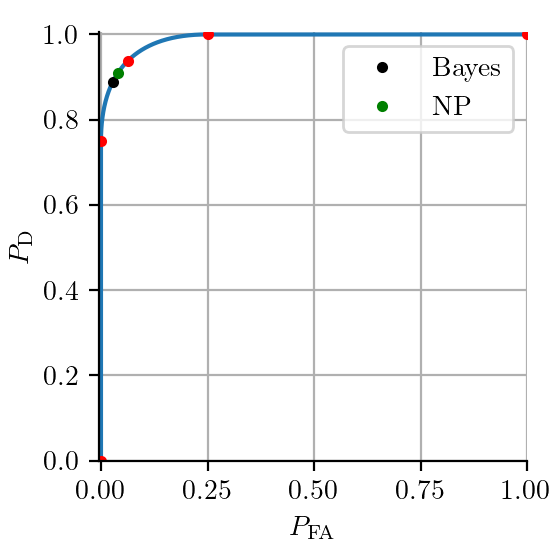
\includegraphics[width=4.5cm]{Figuras/Px06_ROC.png}
\end{center}

\part El decisor bayesiano se corresponde con el caso $\alpha= \frac56$. El decisor NP es el caso $\alpha=0.8$. Sus respectivas posiciones en la ROC se indican en la figura.
\end{parts}
\end{solution}

\else

\question Consider a binary decision problem with $P_H(1) = 2 P_H(0)$ and likelihoods:
$$
\begin{array}{ll} 
	p_{X|H}(x | 0) = 2(1- x),  & 0 \leq x \leq 1  \\
	p_{X|H}(x | 1) = 2 x - 1,  & \dfrac{1}{2} \leq x \leq  \dfrac{3}{2}		  
\end{array}
$$
\begin{parts}
\part Find the Bayesian decision-maker for cost policy $c_{00}=c_{11}=0$, $c_{10}=4c_{01}$.
\part Determine the Neyman-Pearson classifier with $P_{\rm FA} = 0.04$.
\part Obtain, as a function of parameter $\alpha$, the false alarm and detection probabilities for the family of decision-makers with analytic shape
	 $$x \dunodcero \alpha$$
\part Plot (in an approximate manner) the operating characteristic (ROC) curve, taking $\alpha$ as the free parameter, and illustrating how the operation point of the decision-maker changes as a function of the value of such parameter.
\part Indicate whether the decision-makers obtained in (a) and (b) correspond to certain operation points of the previous ROC and, if so, identify it (or them).

\end{parts}

\begin{solution}

\begin{parts}
\part The Bayesian decision-maker for the given costs is given by the decision rule
\begin{align*}
(c_{01} &- c_{11}) P_H(1) p_{X|H}(x|1) \dunodcero (c_{10} - c_{00}) P_H(0) p_{X|H}(x|0) \\
	& \Leftrightarrow \quad c_{01} 2 P_H(0) p_{X|H}(x|1) \dunodcero 4 c_{01} P_H(0) p_{X|H}(x|0) \\
	& \Leftrightarrow \quad p_{X|H}(x|1) \dunodcero 2 p_{X|H}(x|0) \\
	& \Leftrightarrow \quad 
	      \left[\begin{array}{ll}
		        D = 0,                   & \text{if } 0 \le x \le \frac12 \\
		        2 x-1 \dunodcero 4(1-x), & \text{if } \frac12 \le x \le 1 \\
		        D = 1,                   & \text{if } 1 \le x \le \frac32
		        \end{array}
		  \right.   \\
	& \Leftrightarrow \quad 
	      \left[\begin{array}{ll}
		            D = 0,                 & \text{if } 0 \le x \le \frac12 \\
		            x \dunodcero \frac56,  & \text{if } \frac12 \le x \le 1 \\
		            D = 1,                 & \text{if } \frac32 \le x \le 1  
		         \end{array}
		  \right.   \\
	& \Leftrightarrow \quad 
	      x \dunodcero \frac56
\end{align*}
\part The LRT for threshold $\lambda \ge 0$ has the form
\begin{align*}
p_{X|H}(x|1) \dunodcero \lambda p_{X|H}(x|0)
  & \Leftrightarrow \quad 
	  \left[\begin{array}{ll}
            D = 0,                          & \text{if } 0 \le x \le \frac12 \\
		    2x-1 \dunodcero 2\lambda (1-x), & \text{if } \frac12 \le x \le 1 \\
		    D = 1,                          & \text{if } 1 \le x \le \frac32
		    \end{array}
	  \right.   \\
  & \Leftrightarrow \quad 
      \left[\begin{array}{ll}
  	      D = 0,                                        & \text{if } 0 \le x \le \frac12 \\
  	      x \dunodcero \frac{2\lambda+1}{2(1+\lambda)}, & \text{if } \frac12 \le x \le 1 \\
  	      D = 1,                                        & \text{if } 1 \le x \le \frac32
  	      \end{array}
  	  \right.   \\
  & \Leftrightarrow \quad x \dunodcero \alpha
\end{align*}
where $\alpha = \frac{2 \lambda + 1}{2(1+\lambda)} \in [\frac12, 1]$. The false alarm probability is
\begin{align*}
P_{\rm FA} &= P_{D|H}(1|0) 
            = P\{x \ge \alpha | H=0\} \\
           &= \int_\alpha^\infty p_{X|H}(x|0) dx 
            = \int_\alpha^1 2(1-x) dx \\
           &= (1-\alpha)^2
\end{align*}
Taking $P_{\rm FA}\le 0.04$, we get $(1-\mu)^2 = 0.04$, thus $\mu=0.8$ and the NP decision-maker is
\begin{align*}
x \dunodcero 0.8
\end{align*}

\part According to part (b), the false alarm probability, for any $\alpha \in [0, \frac32]$ is
\begin{align*}
P_{\rm FA} 
  &= \left[\begin{array}{ll} 
	       (1-\alpha)^2  & \quad 0 < \alpha < 1         \\
	       0             & \quad 1 < \alpha < \frac32
  	       \end{array}  
  	 \right.  
\end{align*}
In a similar way, the detection probability is
\begin{align*}
P_{\rm D} 
	&= P_{D|H}(1|1) 
     = P\{x \le \alpha | H=1 \}              
     = \int_\alpha^\infty p_{X|H}(x|1) dx  \\
    &= \left[\begin{array}{ll} 
			 1                              & \quad 0 < \alpha < \frac12 \\	  
			 \int_\alpha^\frac32 (2x-1) dx  & \quad \frac12 < \alpha < \frac32
  			 \end{array}  
	   \right.  	 \\
    &= \left[\begin{array}{ll} 
			 1                                  & \quad 0 < \alpha < \frac12	\\	  
			 1 - \left(\alpha-\frac12\right)^2  & \quad \frac12 < \alpha < \frac32   
  			 \end{array}  
	   \right.  	
\end{align*}

\part Obtaining some sample points and plotting the ROC in an approximate manner will suffice. For instance:
\begin{align*}
\begin{array}{llll} 
  \alpha=0       & \Rightarrow & P_{\rm FA}=1,       & P_{\rm D}= 1 \\
  \alpha=\frac12 & \Rightarrow & P_{\rm FA}=\frac14, & P_{\rm D}= 1 \\
  \alpha=\frac34 & \Rightarrow & P_{\rm FA}=\frac14, & P_{\rm D}= \frac{15}{16} \\
  \alpha=1       & \Rightarrow & P_{\rm FA}=0,       & P_{\rm D}= \frac34 \\
  \alpha=\frac32 & \Rightarrow & P_{\rm FA}=0,       & P_{\rm D}= 0
\end{array}
\end{align*}

\begin{center}
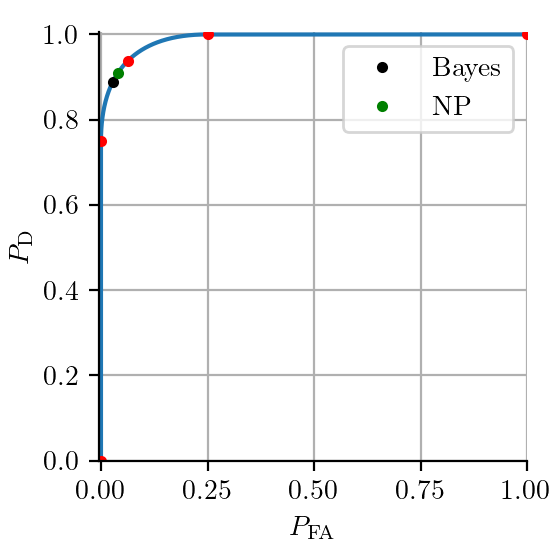
\includegraphics[width=4.5cm]{Figuras/Px06_ROC.png}
\end{center}

\part The Bayesian decision maker is equivalent $\alpha= \frac56$. The NP decision-maker is equivalent to $\alpha=0.8$. Their respective locations in the ROC are shown in the figure.
\end{parts}
\end{solution}

\fi

%%%%%%%%%%%%%%%%%%%%%%%%%%%%%%%%%%%%%%%%%%%%%%%%%%%%%%%%%%%%%%%%%%%
% Examen TDI Enero 2009 T1
\qformat{\textbf{\ej \thequestion ~~ (2.3)} ~~ \linefill}
\ifspanish

\question Se tiene un problema de clasificación binaria bidimensional definido por las siguientes verosimilitudes:
 $$ \begin{array}{l} 
					   p_{X_1,X_2|H}(x_1,x_2 | 0) = G \left( {\bf 0}, \left[ \begin{array}{cc}  
					   1 & \rho \\ \rho & 1					   
					    \end{array}  \right] \right)\\ \\
					  p_{X_1,X_2|H}(x_1,x_2 | 1) = G \left( {\bf m}, \left[ \begin{array}{cc}  
					   1 & \rho \\ \rho & 1					   
					    \end{array}  \right] \right)	  
  \end{array}$$
Represéntese en el plano $X_1-X_2$ la frontera de decisión que proporciona el decisor MAP cuando se satisfacen las siguientes condiciones: $P_H(0)= P_H (1)$, $v_0=v_1$ y $\rho=0$.
Indique cómo se modificaría la frontera anterior si:
\begin{parts}
\part Las probabilidades a priori fuesen $P_H(0)= 2 P_H(1)$.
\part Se incrementase el valor de $\rho$.
\end{parts}
\begin{solution} 
La frontera es la mediatriz de la recta que une los centros de las dos gaussianas.
\begin{parts}
\part Si la $P_H(0)$ es mayor, la recta se desplaza hacia la verosimilitud de $H=1$, es decir, hacia el punto ${\bf m}$.
\part No varía.
\end{parts}
\end{solution}

\else

\question Let the following likelihoods characterize a bidimensional binary decision problem:
 $$ \begin{array}{l} 
					   p_{X_1,X_2|H}(x_1,x_2 | 0) = G \left( {\bf 0}, \left[ \begin{array}{cc}  
					   1 & \rho \\ \rho & 1					   
					    \end{array}  \right] \right)\\ \\
					  p_{X_1,X_2|H}(x_1,x_2 | 1) = G \left( {\bf m}, \left[ \begin{array}{cc}  
					   1 & \rho \\ \rho & 1					   
					    \end{array}  \right] \right)	  
  \end{array}$$
Plot in plane $X_1-X_2$ the decision border given by the MAP decider, if the following conditions hold: $P_H(0)= P_H (1)$, $v_0=v_1$ and $\rho=0$. Indicate how that decision border would change if:
\begin{parts}
\part The {\em a priori} probabilities were $P_H(0)= 2 P_H(1)$.
\part The value of $\rho$ were increased.
\end{parts}

\begin{solution}
The decision border is the bisector of the segment joining the means of both Gaussian distributions.
\begin{parts}
\part If $P_H(0)$ gets larger, then the decision border is shifted towards the likelihood of hypothesis $H=1$, i.e., towards ${\bf m}$.
\part The decision border does not change.
\end{parts}
\end{solution}

\fi

%%%%%%%%%%%%%%%%%%%%%%%%%%%%%%%%%%%%%%%%%%%%%%%%%%%%%%%%%%%%%%%%%%%
% Examen TDI Enero 2009 P1
\qformat{\textbf{\ej \thequestion ~~ (2.2; 2.3; 2.6)} ~~ \linefill}
\ifspanish

\question En un problema de clasificación binaria se sabe que las observaciones presentan distribuciones discretas de Bernoulli con parámetros $p_0$ y $p_1$ ($0 < p_0 < p_1 < 1$):
 $$ P_{X|H}(x | 0) = \left\lbrace  \begin{array}{ll}  
					   p_0 & x=1 \\ 1-p_0 & x=0 \\0 & \mbox{en el resto}					   
					    \end{array}  \right.  \quad \quad \quad 
P_{X|H}(x | 1) = \left\lbrace  \begin{array}{ll}  
					   p_1 & x=1 \\ 1-p_1 & x=0 \\0 & \mbox{en el resto}					   
					    \end{array}  \right.			$$		    
					    
Para la toma de la decisión se dispone de un conjunto de $K$ observaciones independientes y tomadas bajo la misma hipótesis:  $\left\lbrace X^{(k)} \right\rbrace_{k=1}^K$. Se define el siguiente estadístico de las observaciones:  $T=\sum_{k=1}^K X^{(k)}$, i.e., la variable aleatoria $T$ es igual al número de observaciones que son igual a la unidad.
\begin{parts}
\part Obténgase el decisor ML basado en el conjunto de observaciones   $\left\lbrace X^{(k)} \right\rbrace_{k=1}^K$. Exprésese el resultado en función de la v.a. $T$.
\part Sabiendo que la media y la varianza de una distribución Bernoulli con parámetro $p$  valen $p$  y  $p(1-p)$, respectivamente, determínense las medias y varianzas del estadístico $T$ bajo ambas hipótesis: $m_0$ y $v_0$ (para $H=0$) y $m_1$ y $v_1$ (para $H=1$).
\end{parts}
Considérese para el resto del ejercicio $p_0 =1 - p_1$. \\
Para $K$ suficientemente grande, se decide aproximar la v.a. $T$ mediante una distribución Gaussiana, tomando las medias y varianzas calculadas en el apartado anterior. 
\begin{parts}
\setcounter{partno}{2}
\part Calcúlense las $P_{\rm FA}$ y $P_{\rm M}$ del decisor de umbral
 $$t \dunodcero \eta$$
en función del valor de $\eta$.  Exprésese el resultado utilizando la función:
$$F(x) = 1- Q(x) = \int_{-\infty}^x \frac{1}{\sqrt{2\pi}} \exp{\left( - \frac{t^2}{2}\right) } \; dt$$
\part Represéntese de forma aproximada la curva ROC del decisor anterior, indicando:
\begin{itemize}
\item Cómo se desplaza el punto de trabajo al aumentar $\eta$.
\item Cómo se modificaría la curva ROC si creciese el número de observaciones disponibles ($K$).
\item Cómo varía la curva ROC si el valor de $p_1$ crece (manteniendo la condición $p_0 =1 - p_1$).
\end{itemize}
\end{parts}
\begin{solution}
\begin{parts}
\part $t \dunodcero  \displaystyle \frac{K \ln{  \displaystyle \frac{1-p_1}{1-p_0}}} {\ln{  \displaystyle \frac{1-p_1}{1-p_0}}-\ln{  \displaystyle \frac{p_1}{p_0}}}=\eta$
\part $\begin{array}{ll}  
m_0=Kp_0 & \quad  \quad   m_1=Kp_1 \\   v_0=Kp_0 \left(1 - p_0 \right) & \quad  \quad  v_1=Kp_1 \left(1 - p_1 \right)				   
\end{array} $
\part 
$ P_{\rm FA}=F \left( \displaystyle \frac{\eta -K (1-p_1) }{\sqrt{K p_1 (1-p_1) }} \right) \quad \quad \quad
P_{\rm M}=1- F \left(  \displaystyle \frac{\eta -Kp_1 }{\sqrt{K p_1 (1-p_1) }} \right) $

\part Se tiene que si $\eta \rightarrow -\infty$, $P_{\rm FA}=0$ y  $P_{\rm D}=0$ y si $\eta \rightarrow \infty$, $P_{\rm FA}=1$ y  $P_{\rm D}=1$.\\
	Al aumentar $K$, aumenta el area bajo la curva ROC.\\
	Al disminuir $p_1$, aumenta el area bajo la curva ROC.
\end{parts}
\end{solution}

\else

\question It is known that in a binary decision problem the observations follow discrete Bernouilli distributions with parameters $p_0$ and $p_1$ ($0 < p_0 < p_1 < 1$):
 $$ P_{X|H}(x | 0) = \left\lbrace  \begin{array}{ll}  
					   p_0 & x=1 \\ 1-p_0 & x=0 \\0 & \mbox{otherwise}					   
					    \end{array}  \right.  \quad \quad \quad 
P_{X|H}(x | 1) = \left\lbrace  \begin{array}{ll}  
					   p_1 & x=1 \\ 1-p_1 & x=0 \\0 & \mbox{otherwise}					   
					    \end{array}  \right.			$$		    
					    
We have access to a set of $K$ independent observations taken under the same hypothesis for the decision process: $\left\lbrace X^{(k)} \right\rbrace_{k=1}^K$. Let $T$ be a statistic defined as the following function of the observations:  $T=\sum_{k=1}^K X^{(k)}$, i.e., random variable $T$ is the number of observations which are equal to one.
\begin{parts}
\part Obtain the ML decider based on the set of observations $\left\lbrace X^{(k)} \right\rbrace_{k=1}^K$, expressing it as a function of r.v. $T$.
\part Taking into consideration that the mean and variance of a Bernouilli distribution with parameter $p$ are given by $p$ and $1-p$, respectively, find the means and variances of statistic $T$ conditioned on both hypotheses: $m_0$ and $v_0$ (for $H=0$) and $m_1$ and $v_1$ (for $H=1$).
\end{parts}
Consider for the rest of the exercise $p_0 =1 - p_1$. \\
For $K$ large enough, the distribution of $T$ can be approximated by means of a Gaussian distribution, using the previously calculated means and variances.
\begin{parts}
\setcounter{partno}{2}
\part Calculate $P_{\rm FA}$ and $P_{\rm M}$ for the threshold decider
 $$t \dunodcero \eta$$
as a function of $\eta$.  Express your result using function:
$$F(x) = 1- Q(x) = \int_{-\infty}^x \frac{1}{\sqrt{2\pi}} \exp{\left( - \frac{t^2}{2}\right) } \; dt$$
\part Provide an approximate representation of the ROC curve of the previous decider, indicating:
\begin{itemize}
\item How the operation point moves when increasing $\eta$.
\item How the ROC curve would be modified if the number of available observations ($K$) increased.
\item How the ROC curve would change if the value of $p_1$ gets larger (keeping condition $p_0 =1 - p_1$).
\end{itemize}
\end{parts}

\begin{solution}
\begin{parts}
\part $t \dunodcero  \displaystyle \frac{K \ln{  \displaystyle \frac{1-p_1}{1-p_0}}} {\ln{  \displaystyle \frac{1-p_1}{1-p_0}}-\ln{  \displaystyle \frac{p_1}{p_0}}}=\eta$
\part $\begin{array}{ll}  
m_0=Kp_0 & \quad  \quad   m_1=Kp_1 \\   v_0=Kp_0 \left(1 - p_0 \right) & \quad  \quad  v_1=Kp_1 \left(1 - p_1 \right)				   
\end{array} $
\part 
$ P_{\rm FA}=F \left( \displaystyle \frac{\eta -K (1-p_1) }{\sqrt{K p_1 (1-p_1) }} \right) \quad \quad \quad
P_{\rm M}=1- F \left(  \displaystyle \frac{\eta -Kp_1 }{\sqrt{K p_1 (1-p_1) }} \right) $

\part If $\eta \rightarrow -\infty$, $P_{\rm FA}=0$ and  $P_{\rm D}=0$; $\eta \rightarrow \infty$ implies $P_{\rm FA}=1$ and $P_{\rm D}=1$.\\
	The area below the ROC curve increases when $K$ gets larger.\\
	The area below the ROC curve increases if $p_1$ is reduced.
\end{parts}
\end{solution}

\fi

%%%%%%%%%%%%%%%%%%%%%%%%%%%%%%%%%%%%%%%%%%%%%%%%%%%%%%%%%%%%%%%%%%%
% Examen TDI/TDS Enero 2009 (convocatoria extraordinaria) T1
\qformat{\textbf{\ej \thequestion ~~ (2.2)} ~~ \linefill}
\ifspanish

\question Considérese un problema de decisión binario con hipótesis $H=0$ y $H=1$ y observación $X$. Cierto decisor adopta $D=1$ si $X$ se encuentra en {cierta} región {${\cal X}_1$} y $D=0$ en caso contrario, obteniendo probabilidades de falsa alarma y detección $P_{\rm FA}$ y $P_{\rm D}$, respectivamente.\\
El decisor opuesto decide \textcolor{blue}{$D'=0$} si $X$ se encuentra en {${\cal X}_1$} y \textcolor{blue}{$D'=1$} en caso contrario, siendo $P_{\rm FA}'$ y $P_{\rm D}'$ sus probabilidades de falsa alarma y detección, respectivamente.  Determínese la relación entre las probabilidades de falsa alarma y detección de ambos decisores.\\
\begin{solution} 
$$P_{\rm FA}'=1-P_{\rm FA} \quad \quad P_{\rm D}'=1-P_{\rm D}$$
\end{solution}

\else

\question Consider a binary decision problem with hypotheses $H=0$ and $H=1$, and observation $X$.  A particular classifier decides $D=1$ if $X$ falls within region $R_1$, and $D=0$ otherwise, obtaining false alarm and detection probabilities $P_{\rm FA}$ and $P_{\rm D}$, respectively.\\
The complementary classifier decides $D=0$ if $X$ is situated inside $R_1$ and $D=1$ otherwise, $P_{\rm FA}'$ and $P_{\rm D}'$ being the associated probabilities of false alarm and detection, respectively.  Find the existing relationship between the probabilities of false alarm and detection of both decision makers.\\

\begin{solution}
$$P_{\rm FA}'=1-P_{\rm FA} \quad \quad P_{\rm D}'=1-P_{\rm D}$$
\end{solution}

\fi

%%%%%%%%%%%%%%%%%%%%%%%%%%%%%%%%%%%%%%%%%%%%%%%%%%%%%%%%%%%%%%%%%%%
% Examen TDI/TDS Enero 2009 (convocatoria extraordinaria) P2
\qformat{\textbf{\ej \thequestion ~~ (2.3; 2.6)} ~~ \linefill}
\ifspanish

\question Se tiene un problema de decisión binaria definido por las siguientes verosimilitudes:
	 $$ \begin{array}{l} 
					   p_{X_1,X_2|H}(x_1,x_2 | 0) = G \left( {\bf 0}, \left[ \begin{array}{cc}  
					   1 & \rho \\ \rho & 1					   
					    \end{array}  \right] \right)\\ \\
					  p_{X_1,X_2|H}(x_1,x_2 | 1) = G \left( {\bf m}, \left[ \begin{array}{cc}  
					   1 & \rho \\ \rho & 1					   
					    \end{array}  \right] \right)	  
  \end{array}$$
siendo ${\bf m}=\left[ m,m \right] ^T$, con $m>0$ y $|\rho |<1$.
\begin{parts}
\part Sabiendo que $P_H(0)=P_H(1)$, obténgase el decisor bayesiano de mínima probabilidad de error. Represéntese en el plano $X_1-X_2$ la frontera de decisión obtenida.
\part Sobre el clasificador obtenido en a), compruébese que $Z= X_1+X_2$ es un estadístico suficiente para la decisión. Obténganse las verosimilitudes de $H=0$ y $H=1$ sobre la variable aleatoria $Z$, $p_{Z|H}(z|0)$ y $p_{Z|H}(z|1)$.
\part Calcúlense las probabilidades de falsa alarma, de pérdida y de error del decisor anterior; exprésense estas probabilidades utilizando la función
$$F(x) = 1- Q(x) = \int_{-\infty}^x \frac{1}{\sqrt{2\pi}} \exp{\left( - \frac{t^2}{2}\right) } \; dt$$
\part Analícese cómo varía la probabilidad de error con el valor de $\rho$; para ello, considérense los casos $\rho=-1$, $\rho=0$ y $\rho=1$. Indíquese sobre el plano $X_1-X_2$, para cada valor de $\rho$, cómo se distribuyen las verosimilitudes, y represéntese la frontera de decisión.
\end{parts}
\begin{solution}
\begin{parts}
\part $ x_1+x_2 \dunodcero m$
\part $ t \dunodcero m$ \\ \\  $ p_{Z|H}(z | 0) = G \left( 0, 2(1+\rho) \right) \quad \quad  p_{Z|H}(z | 1) = G \left( 2m, 2(1+\rho) \right) $
\part $ P_{\rm FA}=P_{\rm M}=P_{\rm e}=1-F \left( \displaystyle \frac{m}{\sqrt{2(1+\rho)}}  \right)$
\part $\mbox{Si} \; \rho \rightarrow -1:\: P_{\rm e}=0 
\quad \quad \mbox{Si} \; \rho= 0:\: P_{\rm e}=1-F \left( \displaystyle \frac{m}{\sqrt{2}}  \right) 
\quad \quad \mbox{Si} \; \rho \rightarrow 1:\: P_{\rm e}=1-F \left(\displaystyle \frac{m}{2}  \right)$
\end{parts}
\end{solution}

\else

\question We have a binary decision problem with likelihoods:
	 $$ \begin{array}{l} 
					   p_{X_1,X_2|H}(x_1,x_2 | 0) = G \left( {\bf 0}, \left[ \begin{array}{cc}  
					   1 & \rho \\ \rho & 1					   
					    \end{array}  \right] \right)\\ \\
					  p_{X_1,X_2|H}(x_1,x_2 | 1) = G \left( {\bf m}, \left[ \begin{array}{cc}  
					   1 & \rho \\ \rho & 1					   
					    \end{array}  \right] \right)	  
  \end{array}$$
with ${\bf m} = [m,m]^T$, where $m>0$, and $|\rho |<1$.
\begin{parts}
\part Knowing that $P_H(0)=P_H(1)$, obtain the Bayes' decider incurring in a minimum probability of error.  Plot the obtained decision boundary on the plane $X_1-X_2$.
\part For the classifier obtained in a), verify that $Z= X_1+X_2$ is a sufficient statistic for the decision. Obtain the likelihoods of hypotheses $H=0$ and $H=1$ over random variable  $Z$, $p_{Z|H}(z|0)$ and $p_{Z|H}(z|1)$.
\part Calculate the false alarm, missing, and error probabilities of the previous decider, expressing them in terms of function
$$F(x) = 1- Q(x) = \int_{-\infty}^x \frac{1}{\sqrt{2\pi}} \exp{\left( - \frac{t^2}{2}\right) } \; dt$$
\part Analyze how the probability of error changes with $\rho$; in order to do so, consider cases $\rho=-1$, $\rho=0$ , and $\rho=1$. Indicate, for each of these values of $\rho$, how the likelihoods and decision boundary look like on the plane with coordinate axis $X_1-X_2$.
\end{parts}

\begin{solution}
\begin{parts}
\part $ x_1+x_2 \dunodcero m$
\part $ z \dunodcero m$ \\ \\  $ p_{Z|H}(z | 0) = G \left( 0, 2(1+\rho) \right) \quad \quad  p_{Z|H}(z | 1) = G \left( 2m, 2(1+\rho) \right) $
\part $ P_{\rm FA}=P_{\rm M}=P_{\rm e}=1-F \left( \displaystyle \frac{m}{\sqrt{2(1+\rho)}}  \right)$
\part $\mbox{If} \; \rho \rightarrow -1:\: P_{\rm e}=0 
\quad \quad \mbox{If} \; \rho= 0:\: P_{\rm e}=1-F \left( \displaystyle \frac{m}{\sqrt{2}}  \right) 
\quad \quad \mbox{If} \; \rho \rightarrow 1:\: P_{\rm e}=1-F \left(\displaystyle \frac{m}{2}  \right)$
\end{parts}
\end{solution}

\fi

%%%%%%%%%%%%%%%%%%%%%%%%%%%%%%%%%%%%%%%%%%%%%%%%%%%%%%%%%%%%%%%%%%%
% Examen TDI/TDS Septiembre 2008  T1
\qformat{\textbf{\ej \thequestion ~~ (2.1)} ~~ \linefill}
\ifspanish

\question Un problema de decisi\'{o}n ternario unidimensional con hip\'{o}tesis equiprobables est\'{a} definido por las siguientes verosimilitudes:
$$					  \begin{array}{ll}
					  p_{X|H}(x|0) = 2(1-2|x-\displaystyle \frac{1}{2}|), & \quad	0<x<1 \\
					  p_{X|H}(x|1) = 1, &     \quad	0<x<1 \\
					  p_{X|H}(x|2) = 2x, &     \quad	0<x<1
					  \end{array}
					  $$
\begin{parts}
\part Determine el decisor de m\'{\i}nima probabilidad de error.			
\part Discuta si el decisor anterior es equivalente al constituido por un primer decisor de m\'{\i}nima probabilidad de error que elige entre $H={0}$ y $\left\lbrace  H=1 \cup  H=2\right\rbrace  $, y tras ello, caso de aceptar la hip\'{o}tesis $\left\lbrace  H=1 \cup  H=2\right\rbrace  $, se aplica un segundo decisor, tambi\'{e}n de m\'{\i}nima probabilidad de error, para decidir entre $H=1$ y $H=2$.
\end{parts}
\begin{solution}
\begin{parts}
\part $\left\lbrace  \begin{array}{ll} 
					  D=1:& \quad	0<x<\displaystyle 1/4 \\ 
					  D=0:&    \quad	1/4<x<\displaystyle 2/3 \\ 
					  D=2&     \quad	2/3 <x<1 \end{array}  \right. $
\part 
$ \left\lbrace  \begin{array}{ll}
					  D=1:& \quad	0<x<  1/2 \\
					  D=2&     \quad	1/2 <x<1
					  \end{array}  \right.   $ \hspace{2cm}   Es distinto y peor que el anterior
\end{parts}
\end{solution}

\else

\question A unidimensional classification problem involves three ({\em a priori}) equally probable hypotheses, which are characterized by the following likelihoods:
$$					  \begin{array}{ll}
					  p_{X|H}(x|0) = 2\left(1-2\left|x-\displaystyle \frac{1}{2}\right|\right), & \quad	0<x<1 \\
					  p_{X|H}(x|1) = 1, &     \quad	0<x<1 \\
					  p_{X|H}(x|2) = 2x, &     \quad	0<x<1
					  \end{array}
					  $$
\begin{parts}
\part Determine the decision maker that provides a minimum probability of error.		
\part Discuss whether the previous decision maker is equivalent or not to a second decision maker operating in two stages: The first stage classifier decides, with minimum probability of error, between $H={0}$ and $\left\lbrace  H=1 \cup  H=2\right\rbrace  $; then, if hypothesis $\left\lbrace  H=1 \cup  H=2\right\rbrace  $ is selected, a second decision maker is applied to discriminate, again minimizing the probability of error, between $H=1$ and $H=2$.
\end{parts}

\begin{solution}
\begin{parts}
\part $\left\lbrace  \begin{array}{ll} 
					  D=1:& \quad	0<x<\displaystyle 1/4 \\ 
					  D=0:&    \quad	1/4<x<\displaystyle 2/3 \\ 
					  D=2&     \quad	2/3 <x<1 \end{array}  \right. $
\part 
$ \left\lbrace  \begin{array}{ll}
					  D=1:& \quad	0<x<  1/2 \\
					  D=2&     \quad	1/2 <x<1
					  \end{array}  \right.   $ \hspace{.5cm}   Different and worse than the classifier in Part (a).
\end{parts}
\end{solution}

\fi

%%%%%%%%%%%%%%%%%%%%%%%%%%%%%%%%%%%%%%%%%%%%%%%%%%%%%%%%%%%%%%%%%%%
% Examen TDI Septiembre 2008  P1
\qformat{\textbf{\ej \thequestion ~~ (2.3)} ~~ \linefill}
\ifspanish

\question Las verosimilitudes
	 $$ \begin{array}{l} 
					   p_{{\bf X}|H}({\bf x} | 0) = G \left( {\bf 0}, v {\bf I} \right)\\ \\
					  p_{{\bf X}|H}({\bf x} | 1) = G \left( {\bf m}, v {\bf I} \right)	  
  \end{array}$$ 
 
donde ${\bf 0}$ y ${\bf m}$ son vectores $N$-dimensionales de componentes $0$ y $ \left\lbrace m_n \right\rbrace$, respectivamente, e ${\bf I}$ la matriz unitaria $N$x$N$, corresponden a las observaciones $X$ ($N$-dimensionales) en un problema de decisión binaria (gaussiano).
\begin{parts}
\part Disé\~{n}ese el decisor ML.
\part Si $P_H(0)=1/4$, dise\~nese el decisor de mínima probabilidad de error.
\part Calcúlense $P_{\rm FA}$ y $P_{\rm M}$ para el decisor ML. ?`Qué ocurre si crece el número de dimensiones y $ \left\lbrace m_n \right\rbrace \neq 0$?
\part Si en la práctica se tiene acceso a 
$$Z={\bf m}^T{\bf X}+ N$$
donde $N$ es $G(m',v_n)$ e independiente de ${\bf X}$, en lugar de a las observaciones ${\bf X}$, ?`cómo ha de modificarse el dise\~{n}o del decisor ML?
\part Calcúlense $P'_{FA}$ y $P'_M$ para el dise\~{n}o del apartado d). ?`Cómo varían respecto a $P_{\rm FA}$ y $P_{\rm M}$?
\end{parts}
Nota: Utilícese, cuando convenga, la función:
$$F(x) = 1- Q(x) = \int_{-\infty}^x \frac{1}{\sqrt{2\pi}} \exp{\left( - \frac{t^2}{2}\right) } \; dt$$
 
\begin{solution}
\begin{parts}
\part $ {\bf m}^T{\bf X} \dunodcero \displaystyle \frac{1}{2} ||{\bf m}||_2^2$
\part $ {\bf m}^T{\bf X} \dunodcero \displaystyle \frac{1}{2} ||{\bf m}||_2^2-v\ln3$
\part $P_{\rm FA}=P_{\rm M}=F \left( \displaystyle  -\frac{ ||{\bf m}||_2}{2 \sqrt{v}} \right) $, tiende a $0$ cuando $N$ se hace infinito.
\part 
$ z \dunodcero \displaystyle  \frac{1}{2} ||{\bf m}||_2^2 + m'$
\part 
$P'_{FA}=P'_M=F \left( -\displaystyle  \frac{ ||{\bf m}||_2}{2 \sqrt{v+ \displaystyle  \frac{v_n}{||{\bf m}||_2^2}}} \right) $ y crecen con  $\displaystyle  \frac{v_n}{||{\bf m}||_2^2}$. 

\end{parts}
\end{solution}

\else

\question Consider an $N$-dimensional binary (and Gaussian) decision problem, where observation vectors $\bf X$ are distributed according to likelihoods
	 $$ \begin{array}{l} 
					   p_{{\bf X}|H}({\bf x} | 0) = G \left( {\bf 0}, v {\bf I} \right)\\ \\
					  p_{{\bf X}|H}({\bf x} | 1) = G \left( {\bf m}, v {\bf I} \right)	  
  \end{array}$$ 
 where ${\bf 0}$ and ${\bf m}$ are $N$-dimensional vectors with components $0$ and $ \left\lbrace m_n \right\rbrace$, respectively, and ${\bf I}$ is the $N$x$N$ unitary matrix.
\begin{parts}
\part Design the ML classifier.
\part If $P_H(0) = 1/4$, design the minimum probability of error classifier.
\part Obtain $P_{\rm FA}$ and $P_{\rm M}$ for the ML classifier. What behavior would be observed if the number of observations grows with $ \left\lbrace m_n \right\rbrace \neq 0$?
\part In practice, we just have access to random variable $Z$, which is related to $\bf X$ via
$$Z={\bf m}^T{\bf X}+ N$$
where $N$ is $G(m',v_n)$ and independent of ${\bf X}$.  What would the new ML classifier based on the observation of $Z$ be like?
\part Calculate $P'_{FA}$ and $P'_M$ for the design in part d).  How do they change with respect to $P_{\rm FA}$ and $P_{\rm M}$?
\end{parts}
Indication: When, convenient, express your result using function:
$$F(x) = 1- Q(x) = \int_{-\infty}^x \frac{1}{\sqrt{2\pi}} \exp{\left( - \frac{t^2}{2}\right) } \; dt$$
 
\begin{solution}
\begin{parts}
\part $ {\bf m}^T{\bf X} \dunodcero \displaystyle \frac{1}{2} ||{\bf m}||_2^2$
\part $ {\bf m}^T{\bf X} \dunodcero \displaystyle \frac{1}{2} ||{\bf m}||_2^2 - v \ln 3$
\part $P_{\rm FA}=P_{\rm M}=F \left( \displaystyle  \frac{ ||{\bf m}||_2}{2 \sqrt{v}} \right) $, which goes to $0$ as $N$ increases towards infinity.
\part 
$ z \dunodcero \displaystyle  \frac{1}{2} ||{\bf m}||_2^2 + m'$
\part 
$P'_{FA}=P'_M=F \left( \displaystyle  \frac{ ||{\bf m}||_2}{2 \sqrt{v+ \displaystyle  \frac{v_n}{||{\bf m}||_2^2}}} \right) $; they increase with  $\displaystyle  \frac{v_n}{||{\bf m}||_2^2}$. 

\end{parts}
\end{solution}

\fi

%%%%%%%%%%%%%%%%%%%%%%%%%%%%%%%%%%%%%%%%%%%%%%%%%%%%%%%%%%%%%%%%%%%
% Examen TDI Junio 2008 P2
\qformat{\textbf{\ej \thequestion ~~ (2.2; 2.4)} ~~ \linefill}
\ifspanish

\question Considérese el problema de decisión binaria descrito por:
  $$ \begin{array}{l} 
					   p_{X_1,X_2|H}(x_1,x_2 | 0) = \left\lbrace   \begin{array}{ll} \alpha x_2 & \quad 0<x_1< \displaystyle \frac{1}{4} \quad 0<x_2<1 \\
					   0 &  \quad  \mbox{en el resto}\end{array} \right.	   \\ \\
					  p_{X_1,X_2|H}(x_1,x_2 | 1) = \left\lbrace   \begin{array}{ll} \beta x_1 & \quad 0<x_1<1 \quad 0<x_2<  \displaystyle \frac{1}{2} \\
					   0 &  \quad  \mbox{en el resto}\end{array} \right.	
  \end{array}$$ 
 \begin{parts}
\part Tras obtener los valores de las constantes $\alpha$ y $\beta$, represéntense las regiones de decisión correspondientes a un decisor LRT. Indíquese cómo varían las regiones de decisión en función del umbral del clasificador. ?`Existe algún valor de dicho umbral para el que el clasificador obtenido sea lineal?
\part Obténganse las densidades de probabilidad marginales de $x_1$ y $x_2$ bajo ambas hipótesis ($H=0$ y $H=1$). ?`Qué relación estadística existe entre $X_1$ y $X_2$?
\part Por sencillez, se decide utilizar un detector de umbral basado en una única observación, de $X_1$ o de $X_2$:
$$ \mbox{DEC1:} \quad x_1 \dunodcero \eta_1 \quad \quad \quad \mbox{DEC2:} \quad x_2 \dceroduno \eta_2$$
Calcúlense las probabilidades de falsa alarma y de detección de los clasificadores DEC1 y DEC2, expresándolas en función de los umbrales de dichos decisores: $\eta_1$ y $\eta_2$, respectivamente.
\part Dibújense las curvas características de operación (ROC) (i.e., las curvas que representan $P_{\rm D}$ en función de $P_{\rm FA}$) correspondientes a los decisores DEC1 y DEC2, y discútase cómo cambia el punto de operación de cada clasificador al modificar el valor del umbral correspondiente.
\part A la luz de los resultados obtenidos, ?`puede concluirse que alguno de los dos decisores propuestos, DEC1 o DEC2, sea superior al otro?.
\end{parts} 

\begin{solution}
\begin{parts}
\part $\alpha=8$ y $\beta=4$. \\
Donde $ p_{X_1,X_2|H}(x_1,x_2 | 0) $ o $ p_{X_1,X_2|H}(x_1,x_2 | 1) $ son nulas se decide la hipótesis contraria. En la región donde ambas hipótesis no son nulas, considerando el LRT dado por $\displaystyle \frac{ p_{X_1,X_2|H}(x_1,x_2 | 0) }{ p_{X_1,X_2|H}(x_1,x_2 | 1) } \dceroduno \eta$, el decisor es:
 $$ 2x_2 - \eta x_1 \dceroduno 0$$
Para $\eta=4$ la frontera es lineal.
\part Las observaciones son independientes entre sí bajo ambas hipótesis. \\
$ p_{X_1|H}(x_1 | 0) = 4,  \quad 0<x_1< \displaystyle\frac{1}{4}  \quad \quad \; \; \;  p_{X_2|H}(x_2 | 0) =2 x_2, \quad 0<x_2<1 $\\
					$  p_{X_1|H}(x_1 | 1) = 2 x_1,  \quad 0<x_1<1 \quad \quad   p_{X_2|H}(x_2 | 1) =2, \quad 0<x_2< \displaystyle \frac{1}{2} $ 

\part 
$ \mbox{DEC1:} \left\lbrace \begin{array}{l}
\;  P_{\rm FA}= \left\lbrace \begin{array}{ll} 1-4\eta_1, & \; 0<\eta_1 < 1/4 \\
0, &  \; 1/4<\eta_1 <1 \end{array} \right.  \\ \\
 \;   P_{\rm D}=1-\eta_1^2, \quad 0<\eta_1 < 1 \end{array} \right. $ 
$ \mbox{DEC2:} \left\lbrace  \begin{array}{ll} 
\;  P_{\rm FA}=\eta_2^2, \quad 0<\eta_2 <1 \\ \\
\;   P_{\rm D}=\left\lbrace \begin{array}{ll} 2\eta_2, & \; 0<\eta_2 < 1/2 \\ 
						1, & \; 1/2 <\eta_2 < 1 \end{array} \right. \end{array} \right. $
\part 
DEC1: $\eta_1=1$ estamos en el punto $P_{\rm FA}=0$ y $P_{\rm D}= 0$, y si $\eta_1=0$ estamos en el punto $P_{\rm FA}=1$ y $P_{\rm D}= 1$.\\
DEC2: $\eta_2=1$ estamos en el punto $P_{\rm FA}=1$ y $P_{\rm D}= 1$, y si $\eta_2=0$ estamos en el punto $P_{\rm FA}=0$ y $P_{\rm D}= 0$.
\part No puede afirmarse que ninguno de los dos sea siempre mejor que el otro.
 		 
\end{parts} 
\end{solution}

\else

\question Consider a binary decision problem characterized by:
  $$ \begin{array}{l} 
					   p_{X_1,X_2|H}(x_1,x_2 | 0) = \left\lbrace   \begin{array}{ll} \alpha x_2 & \quad 0<x_1< \displaystyle \frac{1}{4} \quad 0<x_2<1 \\
					   0 &  \quad  \mbox{otherwise}\end{array} \right.	   \\ \\
					  p_{X_1,X_2|H}(x_1,x_2 | 1) = \left\lbrace   \begin{array}{ll} \beta x_1 & \quad 0<x_1<1 \quad 0<x_2<  \displaystyle \frac{1}{2} \\
					   0 &  \quad  \mbox{otherwise}\end{array} \right.	
  \end{array}$$ 
 \begin{parts}
\part After finding the values of constants $\alpha$ and $\beta$, provide a graphic representation of the decision regions corresponding to an LRT classifier. Indicate how those regions change as a function of the classifier threshold. Can the threshold be set so that the resulting classifier is linear?
\part Obtain the marginal probability density functions of $x_1$ and $x_2$ conditioned on both hypotheses ($H=0$ and $H=1$). What is the existing statistical relationship between $X_1$ and $X_2$?
\part For simplicity, we opt to use a threshold classifier based in just one variable: $X_1$ or $X_2$:
$$ \mbox{DEC1:} \quad x_1 \dunodcero \eta_1 \quad \quad \quad \mbox{DEC2:} \quad x_2 \dceroduno \eta_2$$
Calculate the probabilities of false alarm and detection of classifiers DEC1 and DEC2, expressing them as functions of the thresholds of such classifiers, $\eta_1$ and $\eta_2$, respectively.
\part Plot the ROC curves (i.e., the curves that represent $P_{\rm D}$ as a function of $P_{\rm FA}$), corresponding to deciders DEC1 and DEC2.  Discuss how the operation points of both classifiers change when modifying the corresponding threholds.
\part In the light of the obtained results, can it be concluded that one of the two proposed classifiers, DEC1 or DEC2, always outperforms the other one?
\end{parts} 

\begin{solution}
\begin{parts}
\part $\alpha=8$ and $\beta=4$. \\
We decide the only plausible hypothesis where $ p_{X_1,X_2|H}(x_1,x_2 | 0) $ or $ p_{X_1,X_2|H}(x_1,x_2 | 1) $ are zero. In the region where both likelihoods overlap, considering the LRT given by $\displaystyle \frac{ p_{X_1,X_2|H}(x_1,x_2 | 0) }{ p_{X_1,X_2|H}(x_1,x_2 | 1) } \dceroduno \eta$, the decider is:
 $$ 2x_2 - \eta x_1 \dceroduno 0$$
For $\eta=4$ a linear border is obtained.
\part Observations $X_1$ and $X_2$ are independent under both hypotheses. \\
$ p_{X_1|H}(x_1 | 0) = 4,  \quad 0<x_1< \displaystyle\frac{1}{4}  \quad \quad \; \; \;  p_{X_2|H}(x_2 | 0) =2 x_2, \quad 0<x_2<1 $\\
					$  p_{X_1|H}(x_1 | 1) = 2 x_1,  \quad 0<x_1<1 \quad \quad   p_{X_2|H}(x_2 | 1) =2, \quad 0<x_2< \displaystyle \frac{1}{2} $ 

\part 
$ \mbox{DEC1:} \left\lbrace \begin{array}{l}
\;  P_{\rm FA}= \left\lbrace \begin{array}{ll} 1-4\eta_1, & \; 0<\eta_1 < 1/4 \\
0, &  \; 1/4<\eta_1 <1 \end{array} \right.  \\ \\
 \;   P_{\rm D}=1-\eta_1^2, \quad 0<\eta_1 < 1 \end{array} \right. $ 
$ \mbox{DEC2:} \left\lbrace  \begin{array}{ll} 
\;  P_{\rm FA}=\eta_2^2, \quad 0<\eta_2 <1 \\ \\
\;   P_{\rm D}=\left\lbrace \begin{array}{ll} 2\eta_2, & \; 0<\eta_2 < 1/2 \\ 
						1, & \; 1/2 <\eta_2 < 1 \end{array} \right. \end{array} \right. $
\part 
DEC1: When $\eta_1=1$ the operation point is $P_{\rm FA}=0$ and $P_{\rm D}= 0$; for $\eta_1=0$ the operation point is $P_{\rm FA}=1$ and $P_{\rm D}= 1$.\\
DEC2: When $\eta_2=1$ the operation point is $P_{\rm FA}=1$ and $P_{\rm D}= 1$; for $\eta_2=0$ the operation point is $P_{\rm FA}=0$ and $P_{\rm D}= 0$.
\part None of the classifiers can be stated to always outperform the other.
 		 
\end{parts} 
\end{solution}

\fi

%%%%%%%%%%%%%%%%%%%%%%%%%%%%%%%%%%%%%%%%%%%%%%%%%%%%%%%%%%%%%%%%%%%
% Examen TDI Mayo 2008 T1 (convocatoria extraordinaria)
\qformat{\textbf{\ej \thequestion ~~ (2.1)} ~~ \linefill}
\ifspanish

\question En un problema de decisión $M$-aria bidimensional con observaciones ${\bf x}=[x_1, \; x_2]^T$, se comprueba que $p_{X_1|X_2,H}(x_1|x_2,H=j)$ no depende de $j$. Se desea dise\~{n}ar un decisor ML, aunque se sabe que las probabilidades a priori, $ \left\lbrace P_H(j) \right\rbrace_{j=1}^M$ son diferentes. Discútase cuál de los siguientes dise\~{n}os es válido:
\begin{parts}
\part $j^*= \arg \max_j \left\lbrace  p_{X_1|H}(x_1 |j) \right\rbrace$
\part $j^*= \arg \max_j \left\lbrace  p_{X_2|H}(x_2 |j) \right\rbrace$
\part $j^*= \arg \max_j \left\lbrace  p_{X_2,H}(x_2, j) \right\rbrace$
\end{parts}

\begin{solution} (b)
\end{solution}

\else

\question Consider an $M$-ary bidimensional classification problem with observations ${\bf x}=[x_1, \; x_2]^T$, where it is known that $p_{X_1|X_2,H}(x_1|x_2,H=j)$ does not depend on $j$ (i.e., on the hypothesis). We want to design the ML classifier.  If it is further known that $ \left\lbrace P_H(j) \right\rbrace_{j=1}^M$ are different, discuss which of the following classifiers provides the ML one:
\begin{parts}
\part $j^*= \arg \max_j \left\lbrace  p_{X_1|H}(x_1 |j) \right\rbrace$
\part $j^*= \arg \max_j \left\lbrace  p_{X_2|H}(x_2 |j) \right\rbrace$
\part $j^*= \arg \max_j \left\lbrace  p_{X_2,H}(x_2, j) \right\rbrace$
\end{parts}

\begin{solution} (b) \end{solution}

\fi

%%%%%%%%%%%%%%%%%%%%%%%%%%%%%%%%%%%%%%%%%%%%%%%%%%%%%%%%%%%%%%%%%%%
% Examen TDI Mayo 2008 P1 (convocatoria extraordinaria)
\qformat{\textbf{\ej \thequestion ~~ (2.1)} ~~ \linefill}
\ifspanish

\question Se conocen las d.d.p. de tres variables aleatorias independientes: 
\begin{align*}
p_{X_1}(x_1) &= \left\lbrace  
	\begin{array}{ll} 1, & 0 \le x_1 \le 1 \\
 	0, & \mbox{en el resto}    \end{array}      
 	\right. \\
p_{X_2}(x_2) &= 2\exp \left( -2x_2  \right), \qquad x_2 \ge 0 \\
p_{X_3}(x_3) &= 2\exp \left( 2 \left( x_3-1 \right)   \right), \qquad x_3 \le  1 
\end{align*}

Considerando las hipótesis:
 $$ \begin{array}{ll} 
 H=1: & \quad X=X_1\\
 H=2: & \quad X=X_2\\
 H=3: & \quad X=X_3\\
  \end{array}$$
determine:
\begin{parts}

\part el decisor bayesiano que minimiza el coste medio global cuando las tres hipótesis son equiprobables y la política de costes es $c_{ii}=0$, $i=1, 2, 3$ y $c_{ij}=c$ con $i\neq j$.

\part las probabilidades de decidir $D=i$ dada la hipótesis $H=i$, i.e., $P\{D=i|H=i\}$ para $i=1, 2, 3$.
\end{parts}
Considerando ahora el problema de decisión binaria dado por:
  $$ \begin{array}{ll} 
 H=1: & \quad X=X_1\\
 H=0: & \quad X=X_2+X_3
  \end{array}$$
determine:
\begin{parts}
\setcounter{partno}{2}
\part el correspondiente decisor ML.
\part las probabilidades de falsa alarma, $P\{D=1|H=0\}$, y de pérdidas, $P\{D=0|H=1\}$.
\end{parts}

%%%%%%%%%%%%%%%%
\begin{solution}
\begin{parts}
\part
Dado que los costes son iguales para todos los tipos de error, y el coste de acertar es 0, el decisor bayesiano coincide con el MAP. Por otra parte, dado que las hipótesis son equiprobables, el decisor MAP coindice con el ML.

De acuerdo con el enunciado, se tienen las verosimilitudes
\begin{align*}
p_{X|H}(x|1) = p_{X_1}(x) \\
p_{X|H}(x|2) = p_{X_2}(x) \\
p_{X|H}(x|3) = p_{X_3}(x) 
\end{align*}
que se representan en la figura.
\begin{center}
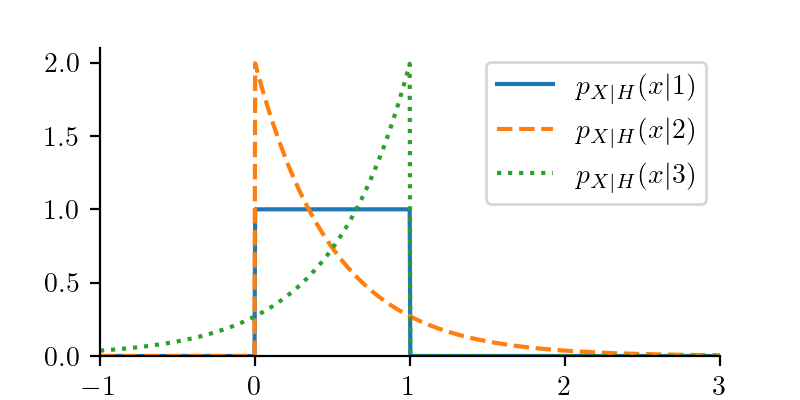
\includegraphics[width=8cm]{Figuras/Px15_3class_likelihoods.png}
\end{center}

El punto de corte de las verosimilitudes de las hipótesis 1 y 2 está dado por la solución de 
\begin{align*}
p_{X|H}&(x|1) = p_{X|H}(x|2)  \\
   &\Leftrightarrow  1 = 2\exp(-2x) \\
   &\Leftrightarrow  x = \frac{\ln(2)}{2} \approx 0.35 
\end{align*}
Del mismo modo (y también por la simetría de  las distribuciones, es inmediato comprobar que el punto de corte de las verosimilitudes de las hipótesis 1 y 3 es
$$
x = 1 - \frac{\ln(2)}{2} \approx 0.66
$$
por tanto, la regla de decisión del decisor bayesiano será
$$
D = \left[
\begin{array}{ll} 
1, & \quad x \in (0.5 \ln(2), \, 1 - 0.5\ln(2))                 \\
2, & \quad x \in [0, \, 0.5\ln(2)] \cup [1, \, \infty)   \\
3, & \quad x \in (-\infty, \, 0] \cup [1-0.5\ln(2),\, 1]
\end{array}
\right.
$$
\part
\begin{align*}
P\{D=1|H=1\} &= P\{x \in (0.5 \ln(2), \, 1 - 0.5\ln(2)) |H=1\} \\
             &= \int_{0.5 \ln(2)}^{1 - 0.5\ln(2)} 1 \cdot dx \\
             &= 1 - \ln(2) \approx 0.31
\end{align*}
Analogamente
\begin{align*}
P\{D=2|H=2\} &= \int_0^{0.5 \ln(2)} 2\exp(-2x) dx + \int_1^{\infty} 2\exp(-2x) dx  \\
             &= \left[ -\exp(-2x) \right]_0^{0.5 \ln(2)} 
              + \left[ -\exp(-2x) \right]_1^{\infty}  \\
             &= \frac12 + e^{-2} \approx 0.64
\end{align*}
y, por simetría
\begin{align*}
P\{D=3|H=3\} = \frac12 + e^{-2} \approx 0.64
\end{align*}

\part Las verosimilitudes de las nuevas hipótesis son:
\begin{align*}
p_{X|H}(x|0) &= (p_{X_2} \ast p_{X_3})(x) = \exp\left(-2|x - 1|\right)   \\
p_{X|H}(x|1) &= p_{X_1}(x)
\end{align*}
(donde $\ast$ denota el operador de convolución), y se representan en la figura
\begin{center}
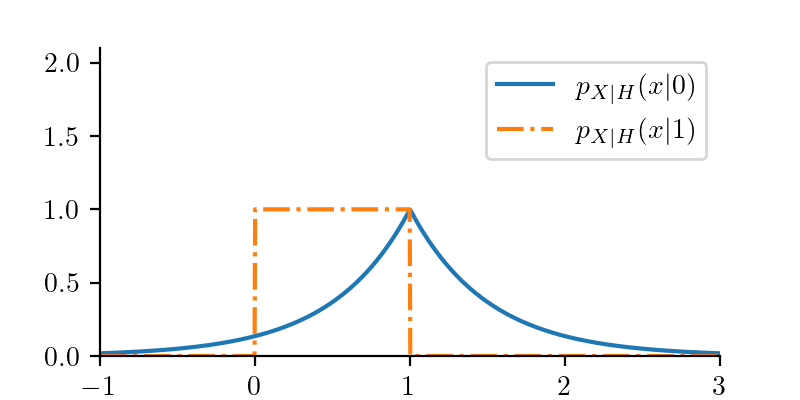
\includegraphics[width=8cm]{Figuras/Px15_2class_likelihoods.png}
\end{center}
Por tanto, el decisor ML será
$$
D = \left[
\begin{array}{ll} 
0, & \quad x \notin    [0, \, 1]    \\
1, & \quad x \in [0, \, 1]
\end{array}
\right.
$$

\part 
\begin{align*}
P_{\rm FA} 
   &= P\{D=1|H=0\} = P\{ 0\le x \le 1 | H=0 \} \\
   &= \int_0^1 \exp(2x-2) dx  
    = \frac12(1 -  e^{-2}) 
    \approx 0.4323
\end{align*}
\begin{align*}
P_{\rm M}=P\{D=0|H=1\} = P\{ x \notin [0, 1] | H=1 \}  = 0
\end{align*}
\end{parts}

\end{solution}
%%%%%%%%%%%%%%

\else

\question Three random variables are characterized by the following likelihoods:
 $$ \begin{array}{l} 
 p_{X_1}(x_1) = \left\lbrace  \begin{array}{ll} 1, & 0 \le x_1 \le 1 \\
 0, & \mbox{otherwise}    \end{array}      \right. \\ \\
 p_{X_2}(x_2) = 2\exp \left( -2x_2  \right), \quad x_2 \ge 0 \\ \\
 p_{X_3}(x_3) = 2\exp \left( 2 \left( x_3-1 \right)   \right), \quad x_3 \le 1 
 \end{array}$$
Considering the following three hypotheses:
 $$ \begin{array}{ll} 
 H=1: & \quad X=X_1\\
 H=2: & \quad X=X_2\\
 H=3: & \quad X=X_3\\
  \end{array}$$
obtain:
\begin{parts}

\part The Bayesian decision-maker that minimizes the overall mean cost when all hypotheses are {\em a priori} equally probable, and the cost policy is $c_{ii}=0$, $i=1, 2, 3$ and $c_{ij}=c$ with $i\neq j$.
\part Probabilities of deciding $D=i$ given hypothesis $H=i$, i.e., $P\{D=i|H=i\}$ for $i=1, 2, 3$.
\end{parts}
Considering now the binary decision problem characterized by:
  $$ \begin{array}{ll} 
 H=1: & \quad X=X_1\\
 H=0: & \quad X=X_2+X_3
  \end{array}$$
obtain:
\begin{parts}
\setcounter{partno}{2}
\part The corresponding ML decider.
\part The false alarm and missing probabilities, $P\{D=1|H=0\}$ and $P\{D=0|H=1\}$, respectively.
\end{parts}


%%%%%%%%%%%%%%%%
\begin{solution}
\begin{parts}
\part
Since the costs for all types of error are equal and the cost of hitting is 0, the Bayesian decision-maker is MAP. Also, since the hypothesis are equally likely, the MAP decision-maker is also ML.

According to the statement, the likelihoods of the hypothesis are
\begin{align*}
p_{X|H}(x|1) = p_{X_1}(x) \\
p_{X|H}(x|2) = p_{X_2}(x) \\
p_{X|H}(x|3) = p_{X_3}(x) 
\end{align*}
and they are represented in the figure.
\begin{center}
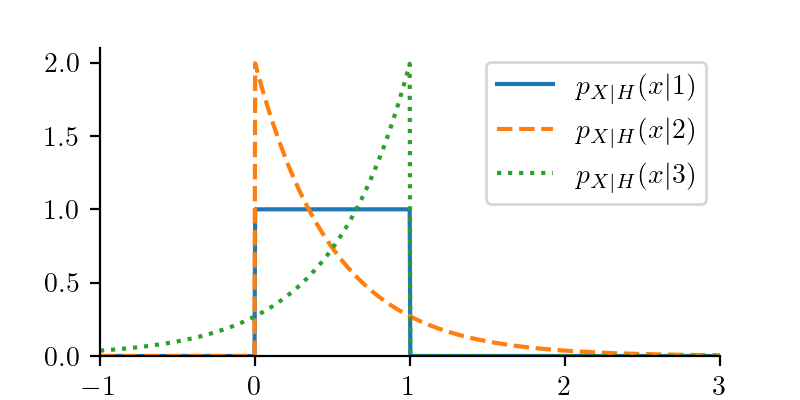
\includegraphics[width=8cm]{Figuras/Px15_3class_likelihoods.png}
\end{center}

The cutting point of the likelihoods for hypotheses 1 and 2 is given by the solution of
\begin{align*}
p_{X|H}&(x|1) = p_{X|H}(x|2)  \\
   &\Leftrightarrow  1 = 2\exp(-2x) \\
   &\Leftrightarrow  x = \frac{\ln(2)}{2} \approx 0.35 
\end{align*}
in the same way (an also because of the symmetry of the distributions) it is straightforward to verify that the cut point of the likelihoods for hypotheses 1 and 3 is
$$
x = 1 - \frac{\ln(2)}{2} \approx 0.66.
$$
Thus, the Bayesian decision rule is
$$
D = \left[
\begin{array}{ll} 
1, & \quad x \in (0.5 \ln(2), \, 1 - 0.5\ln(2))                 \\
2, & \quad x \in [0, \, 0.5\ln(2)] \cup [1, \, \infty)   \\
3, & \quad x \in (-\infty, \, 0] \cup [1-0.5\ln(2),\, 1]
\end{array}
\right.
$$
\part
\begin{align*}
P\{D=1|H=1\} &= P\{x \in (0.5 \ln(2), \, 1 - 0.5\ln(2)) |H=1\} \\
             &= \int_{0.5 \ln(2)}^{1 - 0.5\ln(2)} 1 \cdot dx \\
             &= 1 - \ln(2) \approx 0.31
\end{align*}
Analogamente
\begin{align*}
P\{D=2|H=2\} &= \int_0^{0.5 \ln(2)} 2\exp(-2x) dx + \int_1^{\infty} 2\exp(-2x) dx  \\
             &= \left[ -\exp(-2x) \right]_0^{0.5 \ln(2)} 
              + \left[ -\exp(-2x) \right]_1^{\infty}  \\
             &= \frac12 + e^{-2} \approx 0.64
\end{align*}
y, por simetría
\begin{align*}
P\{D=3|H=3\} = \frac12 + e^{-2} \approx 0.64
\end{align*}

\part The likelihoods for the new hypotheses are:
\begin{align*}
p_{X|H}(x|0) &= (p_{X_2} \ast p_{X_3})(x) = \exp\left(-2|x - 1|\right)   \\
p_{X|H}(x|1) &= p_{X_1}(x)
\end{align*}
(where $\ast$ denotes the convolution operator), and they are represented in the figure
\begin{center}
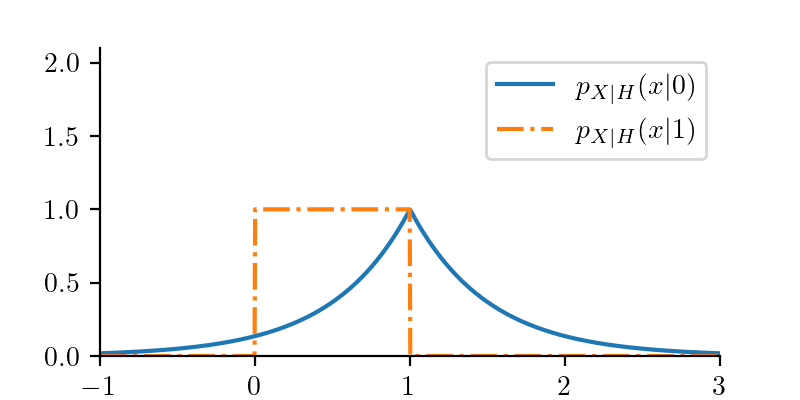
\includegraphics[width=8cm]{Figuras/Px15_2class_likelihoods.png}
\end{center}
Thus, the ML decision-maker is
$$
D = \left[
\begin{array}{ll} 
0, & \quad x \notin    [0, \, 1]    \\
1, & \quad x \in [0, \, 1]
\end{array}
\right.
$$

\part 
\begin{align*}
P_{\rm FA} 
   &= P\{D=1|H=0\} = P\{ 0\le x \le 1 | H=0 \} \\
   &= \int_0^1 \exp(2x-2) dx  
    = \frac12(1 -  e^{-2}) 
    \approx 0.4323
\end{align*}
\begin{align*}
P_{\rm M}=P\{D=0|H=1\} = P\{ x \notin [0, 1] | H=1 \}  = 0
\end{align*}
\end{parts}

\end{solution}
%%%%%%%%%%%%%%

\fi

%%%%%%%%%%%%%%%%%%%%%%%%%%%%%%%%%%%%%%%%%%%%%%%%%%%%%%%%%%%%%%%%%%%
% Examen TDI Febrero 2008 T2
\qformat{\textbf{\ej \thequestion ~~ (2.2)} ~~ \linefill}
\ifspanish

\question Considérese el problema de decisión descrito por las siguientes verosimilitudes:
 $$ \begin{array}{ll} 
 p_{X|H}(x|0) = \left\lbrace  \begin{array}{ll} \displaystyle \frac{2}{a^2} x & 0<x<a \\ \\
 0 & \mbox{en el resto}    \end{array}      \right. & \quad \quad
 p_{X|H}(x|1) = \left\lbrace  \begin{array}{ll} \displaystyle  \frac{1}{a} & 0<x<a \\ \\
 0 & \mbox{en el resto}    \end{array}      \right. 
 \end{array}$$	 
Represéntese la curva característica de operación ($P_{\rm D}$ vs $P_{\rm FA}$) del decisor LRT con un umbral genérico $\eta$. Represéntese sobre dicha curva el punto de trabajo del decisor de máxima verosimilitud.
\begin{solution}
La curva ROC viene dada por la siguiente ecuación: $P_{\rm FA}=P_{\rm D}^2$. \\
El punto de trabajo del decisor ML es: $P_{\rm D}=\displaystyle \frac{1}{2}$ y  $P_{\rm FA}=\displaystyle \frac{1}{4}$
\end{solution}

\else

\question Consider a decision problem characterized by the following likelihoods:
 $$ \begin{array}{ll} 
 p_{X|H}(x|0) = \left\lbrace  \begin{array}{ll} \displaystyle \frac{2}{a^2} x & 0<x<a \\ \\
 0 & \mbox{otherwise}    \end{array}      \right. & \quad \quad
 p_{X|H}(x|1) = \left\lbrace  \begin{array}{ll} \displaystyle  \frac{1}{a} & 0<x<a \\ \\
 0 & \mbox{otherwise}    \end{array}      \right. 
 \end{array}$$	 
Plot the characteristic operation curve ($P_{\rm D}$ vs $P_{\rm FA}$) of the LRT classifier that solves such problem. Place over the curve the operation point corresponding to the maximum likelihood decision maker.

\begin{solution}
The ROC curve is: $P_{\rm FA}=P_{\rm D}^2$. \\
The operation point of the ML classifier is: $P_{\rm D}=\displaystyle \frac{1}{2}$ and  $P_{\rm FA}=\displaystyle \frac{1}{4}$
\end{solution}

\fi

%%%%%%%%%%%%%%%%%%%%%%%%%%%%%%%%%%%%%%%%%%%%%%%%%%%%%%%%%%%%%%%%%%%
% Examen TDI Febrero 2008 P1
\qformat{\textbf{\ej \thequestion ~~ (2.2)} ~~ \linefill}
\ifspanish

\question Un problema de decisi\'{o}n binaria bidimensional viene caracterizado por la equiprobabilidad de las hip\'{o}tesis y por las verosimilitudes
   					$$
					  \begin{array}{ll}
					  p_{X_1,X_2|H}(x_{1},x_{2}|0) = K_{0}x_{1}(1-x_2),& \quad	0<x_1,x_2<1 \\
					  \\
					  p_{X_1,X_2|H}(x_{1},x_{2}|1) = K_{1}x_{1}x_2,&     \quad	0<x_1,x_2<1 \\
					  \end{array}
					  $$
$(K_0,K_1>0)$.
\begin{parts}
 		\part Calc\'{u}lense los valores de las constantes $K_0$ y $K_1$.
 		\part Establ\'{e}zcase el decisor de m\'{\i}nima probabilidad de error, e ind\'{\i}quese el car\'{a}cter de los estad\'{\i}sticos $X_1$ y $X_2$.
 		\part Determ\'{\i}nense las ddp marginales $p_{X_{i}|H}(x_{i}|j)$, $i=1,2$ y $j=0,1$. ¿Qu\'{e} relaci\'{o}n estad\'{\i}stica hay entre $X_1$ y $X_2$ bajo cada hip\'{o}tesis? 
 		\part Calc\'{u}lense $P_{\rm FA}$, $P_{\rm M}$ y $P_{\rm e}$.
 		\part En la pr\'{a}ctica, la medida de $X_2$ viene acompa\~{n}ada de un ruido aditivo $N$ independiente de $X_1$ y $X_2$; es decir, se observa $Y= X_2 + N$. Dis\'{e}\~{n}ese el decisor \'{o}ptimo para esta situaci\'{o}n cuando la ddp de este ruido tiene la forma: 
		$$p(n) = 1, \quad 0<n<1$$
		\part Calc\'{u}lense $P_{\rm FA}'$, $P_{\rm M}'$ y $P_{e}'$ para la situaci\'{o}n y el dise\~{n}o del apartado anterior.
 \end{parts}
\begin{solution}

   \begin{parts}
  \part $K_0=K_1=4$
 \part $x_2 \dunodcero \displaystyle \frac{1}{2}$; 
  $X_1$ es irrelevante para la decisión y $X_2$ es un estadístico suficiente.
   \part $p_{X_1|H}(x_1|0)=2x_1, \; 0<x_1<1; \quad p_{X_1|H}(x_1|1)=2x_1, \; 0<x_1<1$\\
$p_{X_2|H}(x_2|0)=2(1-x_2), \; 0<x_2<1; \quad p_{X_2|H}(x_2|1)=2x_2, \; 0<x_2<1$\\
 $X_1$ y $X_2$ son independientes bajo cada hip\'{o}tesis.
 \part  $P_{\rm FA}=P_{\rm M}=P_{\rm e}=\displaystyle \frac{1}{4}$.
 \part Llamando $Y=X_2+N$, se seguir\'{a} cumpliendo:
 $p_{X_1,Y|H}(x_1,y|i)= p_{X_1|H}(x_1|i)p_{Y|H}(y|i)$, $i=0,1$
 y bastar\'{a} trabajar con $Y$, cuyas ddps (bajo cada hip\'{o}tesis) se obtienen convulocionando las de $X_2$ y de $N$:\\
 $p_{Y|H}(y|0) =
					      \left\{\begin{array}{ll}
						  	\displaystyle
						  	0,&			\quad y<0\\
						  	2y-y^2,&	\quad 0<y<1\\
						  	4-4y+y^2,&	\quad 1<y<2\\
						  	0,&	\quad y>2\\
						   	\end{array}
						   	\right. 
						  	\quad \quad
p_{Y|H}(y|1) =
					      \left\{\begin{array}{ll}
						  	\displaystyle
						  	0,&			\quad y<0\\
						  	y^2,&	\quad 0<y<1\\
						  	2y-y^2,&	\quad 1<y<2\\
						  	0,&	\quad y>2\\
						   	\end{array}
						   	\right. 
						  	$
resultando el decisor: $ y=x_2+n \dunodcero 1$
 \part $P_{\rm FA}'=P_{\rm M}'=P_{\rm e}'=\displaystyle \frac{1}{3}$.
 \end{parts}
 \end{solution}

\else

\question A bidimensional binary decision probability is characterized by equally probable hypotheses, and likelihoods:
   					$$
					  \begin{array}{ll}
					  p_{X_1,X_2|H}(x_{1},x_{2}|0) = K_{0}x_{1}(1-x_2),& \quad	0<x_1,x_2<1 \\
					  \\
					  p_{X_1,X_2|H}(x_{1},x_{2}|1) = K_{1}x_{1}x_2,&     \quad	0<x_1,x_2<1 \\
					  \end{array}
					  $$
$(K_0,K_1>0)$.
\begin{parts}
 		\part Calculate the values of constants $K_0$ and $K_1$.
 		\part Find the classifier that minimizes the probability of error, and indicate the importance of $X_1$ and $X_2$ in the decision process.
 		\part Obtain marginal likelihoods $p_{X_{i}|H}(x_{i}|j)$, for $i=1,2$ and $j=0,1$. What is the statistical relationship between $X_1$ and $X_2$ under each hypothesis? 
 		\part Calculate $P_{\rm FA}$, $P_{\rm M}$ y $P_{\rm e}$.
 		\part In practice, $X_2$ can not be observed directly, but we can just access a version contaminated with an additive noise $N$ independent of $X_1$ and $X_2$; i.e., we observe $Y= X_2 + N$. Design the optimal decider for this situation when the noise pdf is: 
		$$p_N(n) = 1, \quad 0<n<1$$
		\part Calculate $P_{\rm FA}'$, $P_{\rm M}'$ and $P_{e}'$ for the new situation and the classifier designed in part (e).
 \end{parts}

\begin{solution}

   \begin{parts}
  \part $K_0=K_1=4$
 \part $x_2 \dunodcero \displaystyle \frac{1}{2}$; 
  $X_1$ does not provide relevant information for the decision, whereas $X_2$ is a sufficient statistic.
   \part $p_{X_1|H}(x_1|0)=2x_1, \; 0<x_1<1; \quad p_{X_1|H}(x_1|1)=2x_1, \; 0<x_1<1$\\
$p_{X_2|H}(x_2|0)=2(1-x_2), \; 0<x_2<1; \quad p_{X_2|H}(x_2|1)=2x_2, \; 0<x_2<1$\\
 $X_1$ are $X_2$ independent under whatever hypothesis.
 \part  $P_{\rm FA}=P_{\rm M}=P_{\rm e}=\displaystyle \frac{1}{4}$.
 \part With $Y=X_2+N$, it still holds that:
 $p_{X_1,Y|H}(x_1,y|i)= p_{X_1|H}(x_1|i)p_{Y|H}(y|i)$, $i=0,1$
 and we just need to work with $Y$ instead of $X_2$. The likelihoods, expressed as distributions over $Y$, can be obtained by convolving the distributions of $X_2$ and $N$, resulting:\\
 $p_{Y|H}(y|0) =
					      \left\{\begin{array}{ll}
						  	\displaystyle
						  	0,&			\quad y<0\\
						  	2y-y^2,&	\quad 0<y<1\\
						  	4-4y+y^2,&	\quad 1<y<2\\
						  	0,&	\quad y>2\\
						   	\end{array}
						   	\right. 
						  	\quad \quad
p_{Y|H}(y|1) =
					      \left\{\begin{array}{ll}
						  	\displaystyle
						  	0,&			\quad y<0\\
						  	y^2,&	\quad 0<y<1\\
						  	2y-y^2,&	\quad 1<y<2\\
						  	0,&	\quad y>2\\
						   	\end{array}
						   	\right. 
						  	$
The new decider is: $ y=x_2+n \dunodcero 1$
 \part $P_{\rm FA}'=P_{\rm M}'=P_{\rm e}'=\displaystyle \frac{1}{3}$.
 \end{parts}
 
 \end{solution}

\fi
 
%%%%%%%%%%%%%%%%%%%%%%%%%%%%%%%%%%%%%%%%%%%%%%%%%%%%%%%%%%%%%%%%%%%
% Examen TDI/TDS Enero 2008 P1
\qformat{\textbf{\ej \thequestion ~~ (2.2; 2.6)} ~~ \linefill}
\ifspanish

\question Un sistema genera dos observaciones, $X_1$ y $X_2$, que, tanto bajo hipótesis $H=0$ como $H=1$, son independientes e idénticamente distribuidas, siendo
 $$\begin{array}{ll}
 p_{X_i|H}(x_i|1)=2x_i & \quad 0<x_i<1 \\
 p_{X_i|H}(x_i|0)=2(1-x_i) & \quad 0<x_i<1
 \end{array}$$
Suponga hipótesis equiprobables.
\begin{parts}
\part Determine el decisor MAP basado en $X_1$ y calcule su probabilidad de error.
\end{parts}
Sea DMAP1 el decisor del apartado a), suponga que si $|x_1-0.5|<a$ (siendo $0<a<0.5$), se observa $X_2$ y, con objeto de seguir aplicando decisión por umbral, se descartan $X_1$ y la decisión de DMAP1. En su lugar, se aplica un segundo decisor, basado en $X_2$ y también MAP, que llamaremos DMAP2. 
\begin{parts}
\setcounter{partno}{1}
\part Represente gráficamente sobre el plano $X_1-X_2$, para un valor de $a$ arbitrario, las regiones de decisión del esquema conjunto DMAP1-DMAP2.
\part Determine la probabilidad de error global del esquema conjunto DMAP1-DMAP2.
\part Determine la máxima reducción de la probabilidad de error global que puede conseguirse utilizando el esquema conjunto, respecto al decisor DMAP1.
\part Compare las prestaciones del decisor conjunto DMAP1-DMAP2 con las del decisor MAP que utiliza simultáneamente $X_1$ y $X_2$.
\end{parts}
\begin{solution}
\begin{parts}
\part $ x_1 \dunodcero \displaystyle \frac{1}{2} \quad \quad P_{\rm e}=\displaystyle \frac{1}{4}$
\part 
$\begin{array}{ll}
D=0: & \;  x_1<1/2-a	\quad \mbox{y} \quad 1/2-a< x_1<1/2+a,  \; x_2<1/2 \\
D=1: & \;  1/2-a< x_1<1/2+a,  \;  x_2>1/2 	\quad \mbox{y} \quad  x1>1/2+a	\end{array}$
\part $P_{\rm e}=a^2-0.5a+0.25$
\part La variación máxima de la probabilidad de error es $\displaystyle \frac{1}{16}$
\part DMAP($X_1$ y $X_2$): $P_{\rm e}=\displaystyle \frac{1}{6}$ \\
DMAP1- DMAP2: $P_{\rm e}$ varía de $\displaystyle \frac{1}{4}$ a $\displaystyle \frac{1}{16}$
\end{parts}
\end{solution}

\else

\question A system generates two observations $X_1$ and $X_2$ that, under both hypothesis $H=0$ and $H=1$, are independent and identically distributed:
 $$\begin{array}{ll}
 p_{X_i|H}(x_i|1)=2x_i & \quad 0<x_i<1 \\
 p_{X_i|H}(x_i|0)=2(1-x_i) & \quad 0<x_i<1
 \end{array}$$
Assume that the {\em a priori} probability is the same for both hypotheses.
\begin{parts}
\part Determine the MAP decider based on $X_1$, and calculate its probability of error.
\end{parts}
Let DMAP1 be the decider of section a), and assume that if $|x_1-0.5|<a$ (with $0<a<0.5$), $X_2$ is also observed. When this happens, and with the goal of still applying a threshold classifier, $X_1$ is discarded (as well as DMAP1 decision, and a second MAP classifier (DMAP2), based on the observation of $X_2$, is applied. 
\begin{parts}
\setcounter{partno}{1}
\part Plot on plane $X_1-X_2$, for a generic value $a$, the decision regions for the joint scheme DMAP1-DMAP2.
\part Find the probability of error of the joint scheme DMAP1-DMAP2.
\part Find the maximum reduction of the probability of error that can be achieved using the joint scheme, with respect to the probability of error of decider DMAP1.
\part Compare the performance of the joint decider DMAP1-DMAP2 with that of the optimum MAP decider based on the joint observation of $X_1$ and $X_2$.
\end{parts}

\begin{solution}
\begin{parts}
\part $ x_1 \dunodcero \displaystyle \frac{1}{2} \quad \quad P_{\rm e}=\displaystyle \frac{1}{4}$
\part 
$\begin{array}{ll}
D=0: & \;  x_1<1/2-a	\quad \mbox{and} \quad 1/2-a< x_1<1/2+a,  \; x_2<1/2 \\
D=1: & \;  1/2-a< x_1<1/2+a,  \;  x_2>1/2 	\quad \mbox{and} \quad  x_1>1/2+a	\end{array}$
\part $P_{\rm e}=a^2-0.5a+0.25$
\part The maximum reduction of the probability of error is $\displaystyle \frac{1}{16}$
\part DMAP($X_1$ and $X_2$): $P_{\rm e}=\displaystyle \frac{1}{6}$ \\
DMAP1- DMAP2: $P_{\rm e}$ changes from $\displaystyle \frac{1}{4}$ to $\displaystyle \frac{1}{16}$
\end{parts}
\end{solution}

\fi

%%%%%%%%%%%%%%%%%%%%%%%%%%%%%%%%%%%%%%%%%%%%%%%%%%%%%%%%%%%%%%%%%%%
% Examen TDI/TDS Septiembre 2007 P1
\qformat{\textbf{\ej \thequestion ~~ (2.2)} ~~ \linefill}
\ifspanish

\question Considérese el problema de decisión binaria descrito por: 
 $$ p_{X_1,X_2|H}(x_1,x_2|i)= a_i^2 \exp \left(  -a_i \left( x_1+x_2\right) \right) \quad x_1,x_2>0 \quad i=0,1$$
donde $a_0=1$ y $a_1=2$.
\begin{parts}
\part Disé\~{n}ese el decisor MAP correspondiente en función del parámetro $R=P_H(1)/P_H(0)$.
\part Compruébese que $T=X_1+X_2$ es un estadístico suficiente y calcúlense las verosimilitudes de dicho estadístico, $p_{T|H}(t|i) $, $i=0,1$.
\part  Calcúlense las probabilidades de falsa alarma, de pérdida y de error del decisor dise\~{n}ado en (a).
\end{parts}
\begin{solution}
\begin{parts}
\part $\begin{array}{ll}
D=1: & \; x_1+x_2<\ln(4R) \\
D=0: & \; x_1+x_2>\ln(4R)
\end{array}$
\part 
$\begin{array}{ll}
D=1: & \; t<\ln(4R) \\
D=0: & \; t>\ln(4R)
\end{array}$ \\

$ p_{T|H}(t|0)= t \exp \left(-t \right), \quad t>0 \quad \quad \quad  p_{T|H}(t|1)= 4t \exp \left(-2t \right), \quad t>0 $
\part  $ P_{\rm FA}=1-\displaystyle  \frac{1+\ln (4R)}{4R} \quad \quad 
P_{\rm M}= \displaystyle  \frac{1+2\ln (4R)}{(4R)^2}  \quad \quad 
P_{\rm e}= P_H(0) \left( 1- \displaystyle  \frac{3}{16R} -\displaystyle  \frac{1}{8R}\ln(4R)  \right) $
\end{parts}
\end{solution}

\else

\question Consider a binary decision problem characterized by: 
 $$ p_{X_1,X_2|H}(x_1,x_2|i)= a_i^2 \exp \left[  -a_i \left( x_1+x_2\right) \right] \quad x_1,x_2>0 \quad i=0,1$$
where $a_0=1$ and $a_1=2$.
\begin{parts}
\part Design the corresponding MAP decider as a function of parameter $R=P_H(1)/P_H(0)$.
\part Check that $T=X_1+X_2$ is a sufficient statistic, and calculate the likelihoods expressed as probability density functions of such statistic, $p_{T|H}(t|i) $, $i=0,1$.
\part  Calculate the false alarm, missing, and error probabilities of the decider designed in section (a).
\end{parts}

\begin{solution}
\begin{parts}
\part $\begin{array}{ll}
D=1: & \; x_1+x_2<\ln(4R) \\
D=0: & \; x_1+x_2>\ln(4R)
\end{array}$
\part 
$\begin{array}{ll}
D=1: & \; t<\ln(4R) \\
D=0: & \; t>\ln(4R)
\end{array}$ \\

$ p_{T|H}(t|0)= t \exp \left(-t \right), \quad t>0 \quad \quad \quad  p_{T|H}(t|1)= 4t \exp \left(-2t \right), \quad t>0 $
\part  $ P_{\rm FA}=1-\displaystyle  \frac{1+\ln (4R)}{4R} \quad \quad 
P_{\rm M}= \displaystyle  \frac{1+2\ln (4R)}{(4R)^2}  \quad \quad 
P_{\rm e}= P_H(0) \left( 1- \displaystyle  \frac{3}{16R} -\displaystyle  \frac{1}{8R}\ln(4R)  \right) $
\end{parts}
\end{solution}

\fi

%%%%%%%%%%%%%%%%%%%%%%%%%%%%%%%%%%%%%%%%%%%%%%%%%%%%%%%%%%%%%%%%%%%
% Examen TDS Septiembre 2007 P1
\qformat{\textbf{\ej \thequestion ~~ (2.2; 2.5)} ~~ \linefill}
\ifspanish

\question En un problema de decisión binaria con hipótesis equiprobables donde las verosimilitudes de las observaciones son:
 $$\begin{array}{ll}
 p_{X|H}(x|0)=2 \left(1-x \right) & \quad 0<x<1 \\
  p_{X|H}(x|1)=1/a & \quad 0<x<a
 \end{array}$$
siendo $a\geq1$ un parámetro determinista.
\begin{parts}
\part  Considerando que la política de costes viene dada por: $c_{00}=c_{11}=0$ y $c_{01}=c_{10}=1$, disé\~{n}ese el decisor óptimo supuesto que es conocido el valor de $a$.
\end{parts}
Supóngase ahora que el valor de a es desconocido. Se opta por aplicar una estrategia  minimax, fijando para la toma de decisiones un umbral  $x_u^*$ elegido para minimizar el máximo coste medio; es decir, 
 $$x_u^*=\arg \left\lbrace \min_{x_u}  \left\lbrace \max_a C(x_u,a)   \right\rbrace   \right\rbrace  $$
siendo  $x_u$ un umbral de decisión genérico
		 $$x \dunodcero x_u$$
\begin{parts}
\setcounter{partno}{1}
\part Determínese  $x_u^*$.
\part  Calcúlese el incremento del coste medio que se produce al aplicar la estrategia minimax respecto al que se tendría si el valor del parámetro $a$ fuese conocido.
\end{parts}
\begin{solution}
\begin{parts}
\part $ x \dunodcero 1 - \displaystyle \frac{1}{2a} \quad 0<x<a $
\part   $x_u^*=\displaystyle \frac{1}{2}$
\part $ \Delta P_{\rm e} = \displaystyle \frac{1}{8} - \displaystyle \frac{1}{4a} \left( 1- \displaystyle \frac{1}{2a} \right) $
nulo para $a=1$ y positivo para $a>1$.
\end{parts}
\end{solution}

\else

\question Consider a binary decision problem with $P_H(0) = P_H(1)$ and likelihoods:
 $$\begin{array}{ll}
 p_{X|H}(x|0)=2 \left(1-x \right) & \quad 0<x<1 \\
  p_{X|H}(x|1)=1/a & \quad 0<x<a
 \end{array}$$
$a\geq1$ being a deterministic parameter.
\begin{parts}
\part  Design the optimal classifier for cost policy $c_{00}=c_{11}=0$ and $c_{01}=c_{10}=1$, assuming that the value of $a$ is known.
\end{parts}
Assume now that the value of $a$ is not known. We opt to apply a minimax strategy, using a threshold $x_u^*$ for the decision process which is selected to minimize the maximum risk, i.e., 
 $$x_u^*=\arg \left\lbrace \min_{x_u}  \left\lbrace \max_a C(x_u,a)   \right\rbrace   \right\rbrace  $$
where $x_u$ is a generic decision threshold
		 $$x \dunodcero x_u$$
\begin{parts}
\setcounter{partno}{1}
\part Obtain  $x_u^*$.
\part  Find the increment of the risk that would be produced when applying the minimax strategy over the cost that would be obtained if the value of $a$ were known.
\end{parts}

\begin{solution}
\begin{parts}
\part $ x \dunodcero 1 - \displaystyle \frac{1}{2a} \quad 0<x<a $
\part   $x_u^*=\displaystyle \frac{1}{2}$
\part $ \Delta P_{\rm e} = \displaystyle \frac{1}{8} - \displaystyle \frac{1}{4a} \left( 1- \displaystyle \frac{1}{2a} \right) $, which is zero for $a=1$, and positive for $a>1$.
\end{parts}
\end{solution}

\fi

%%%%%%%%%%%%%%%%%%%%%%%%%%%%%%%%%%%%%%%%%%%%%%%%%%%%%%%%%%%%%%%%%%%
% Examen TDI Junio 2007 T2
\qformat{\textbf{\ej \thequestion ~~ (2.3)} ~~ \linefill}
\ifspanish

\question Considérese el problema bidimensional binario Gaussiano 
  $$ \begin{array}{l} 
					   p_{X_1,X_2|H}(x_1,x_2 | 0) = G \left( \left[ \begin{array}{c}  
					   1  \\ 0  \end{array}  \right], 
					   \left[ \begin{array}{cc}  
					   2 & -1 \\ -1 & 2					   
					    \end{array}  \right] \right)\\ \\
					  p_{X_1,X_2|H}(x_1,x_2 | 1) = G \left( \left[ \begin{array}{c}  
					   0  \\ 1  \end{array}  \right], 
					   \left[ \begin{array}{cc}  
					   2 & -1 \\ -1 & 2					   
					    \end{array}  \right] \right)  
  \end{array}$$
Las probabilidades de las hipótesis son $P_H (0) = 2/3$ y $P_H (1) = 1/3$,  y  los costes asociados son $c_{00}= c_{11}=0$, $c_{01}= c_{10}= 1$.
 \begin{parts}
\part Establézcase la expresión que proporciona el correspondiente decisor Bayesiano en función del vector de observaciones ${\bf  X}$.
\part  Represéntese cómo se desplaza la frontera de decisión al variar el valor de $P_H(0)$. 
\end{parts}

\begin{solution}
\begin{parts}
\part $x_2 -x_1 \dunodcero 10 \ln 2$
\part  Si aumenta $P_H(0)$ la frontera se mueve hacia el punto $[0,1]^T$ y  si disminuye $P_H(0)$ la frontera se mueve hacia el punto $[1,0]^T$. 
\end{parts}
\end{solution}

\else

\question Consider a bidimensional Gaussian decision problem
  $$ \begin{array}{l} 
					   p_{X_1,X_2|H}(x_1,x_2 | 0) = G \left( \left[ \begin{array}{c}  
					   1  \\ 0  \end{array}  \right], 
					   \left[ \begin{array}{cc}  
					   2 & -1 \\ -1 & 2					   
					    \end{array}  \right] \right)\\ \\
					  p_{X_1,X_2|H}(x_1,x_2 | 1) = G \left( \left[ \begin{array}{c}  
					   0  \\ 1  \end{array}  \right], 
					   \left[ \begin{array}{cc}  
					   2 & -1 \\ -1 & 2					   
					    \end{array}  \right] \right)  
  \end{array}$$
The {\em a priori} probabilities of the hypotheses are $P_H (0) = 2/3$ and $P_H (1) = 1/3$,  whereas the associated cost policy is $c_{00}= c_{11}=0$, $c_{01}= c_{10}= 1$.
 \begin{parts}
\part Establish the expression that provides the corresponding Bayes' decision as a function of the observation vector ${\bf  X}$.
\part  Show, over a graphic representation, how the decision border changes when varying the value of $P_H(0)$. 
\end{parts}

\begin{solution}
\begin{parts}
\part $x_2 -x_1 \dunodcero 10 \ln 2$
\part  If $P_H(0)$ increases, the border moves towards point $[0,1]^T$, while a reduction in $P_H(0)$ moves the border towards $[1,0]^T$. 
\end{parts}
\end{solution}

\fi

%%%%%%%%%%%%%%%%%%%%%%%%%%%%%%%%%%%%%%%%%%%%%%%%%%%%%%%%%%%%%%%%%%%
% Examen TDI Junio 2007 P1
\qformat{\textbf{\ej \thequestion ~~ (2.2; 2.4)} ~~ \linefill}
\ifspanish

\question Considérese un escenario de decisión radar en el que se sabe que los blancos que se desea detectar pueden causar ecos con dos niveles diferentes de intensidad:
 $$\begin{array}{ll}
 H=0 \; \mbox{(no hay blanco):} & \quad X=N \\
 H=1 \; \mbox{(hay blanco):} & \quad  \left\lbrace   \begin{array}{ll}  H=1a: & \quad X=s_1+N \\  H=1b: & \quad X=s_2+N  \end{array} \right. 
 \end{array} $$
donde los valores reales $s_1$ y $s_2$ son los dos niveles de eco conocidos para cada tipo de blanco, y $N$ es una v.a. con distribución $G(0,1)$.  Se sabe, además, que $P_H(1a|1) = P$ y $P_H(1b|1) = 1-P$ ($0<P<1$).
\begin{parts}
\part Establézcase la forma general del test de razón de verosimilitudes que permite discriminar $H=0$ frente a $H=1$, y justifíquese que si los signos de $s_1$ y $s_2$ coinciden, dicho detector es un detector de un único umbral.
\part	 ?`Existen combinaciones de valores de $s_1$ y $s_2$ para los que un test de máxima verosimilitud decida siempre la misma hipótesis?
\part	 Asumiendo $s_2 < s_1 < 0$ y el siguiente detector de umbral:
 $$ x \dceroduno \eta$$
determínense $P_{\rm FA}$ y $P_{\rm D}$ en función de $\eta$ y exprese su resultado utilizando la función:
$$F(x) = 1- Q(x) = \int_{-\infty}^x \frac{1}{\sqrt{2\pi}} \exp{\left( - \frac{t^2}{2}\right) } \; dt$$
 Represéntese de forma aproximada la curva ROC ($P_{\rm D}$ vs $P_{\rm FA}$ en función de $\eta$) del detector, situando sobre la misma los puntos correspondientes a $\eta \rightarrow \pm \infty$, e indicando cómo varía el punto de trabajo en función del umbral.
\part	Explíquese qué efectos tendrían sobre la ROC: 
\begin{itemize}
\item	 aumentar $s_1$. 
\item	 disminuir $s_2$. 
\item	 aumentar $P$.
\item	 aumentar $P_H(0)$.
\end{itemize}
\end{parts}
\begin{solution}
\begin{parts}
\part $P \exp \left( - \displaystyle \frac{1}{2} \left(  s_1^2-2s_1x   \right) \right) + \left( 1-P \right) \exp \left( - \displaystyle \frac{1}{2} \left(  s_2^2-2s_2x   \right) \right) \dunodcero \eta$
\part No
\part {$P_{\rm FA}=F(\eta)$}, $\quad \quad P_{\rm D}=1-P F(\eta-s_1)- (1-P) F(\eta-s_2) $
\part 
\begin{itemize}
\item aumentar $s_1$: disminuye el area de la ROC
\item disminuir $s_2$: aumenta el area de la ROC
\item aumentar $P$: disminuye el area de la ROC
\item aumentar $P_H(0)$: no afecta
\end{itemize}
	\end{parts}
	\end{solution}

\else

\question Consider a radar detection problem in which the targets can cause echoes with two different intensity levels:
 $$\begin{array}{ll}
 H=0 \; \mbox{(no target):} & \quad X=N \\
 H=1 \; \mbox{(target present):} & \quad  \left\lbrace   \begin{array}{ll}  H=1a: & \quad X=s_1+N \\  H=1b: & \quad X=s_2+N  \end{array} \right. 
 \end{array} $$
where $s_1$ and $s_2$ are real values associated to the two echo levels for the different targets, and $N$ is a r.v. with distribution $G(0,1)$.  It is also known that $P_H(1a|1) = P$ and $P_H(1b|1) = 1-P$ ($0<P<1$).
\begin{parts}
\part Establish the general shape of an LRT which discriminates $H=0$ and $H=1$, and justify that such classifier is a threshold classifier when the signs of $s_1$ and $s_2$ are the same.
\part	 Are there any combination of values of $s_1$ and $s_2$ for which a maximum likelihood test decides always in favor of the same hypothesis?
\part	 Assuming $s_2 < s_1 < 0$ and the following threshold detector:
 $$ x \dceroduno \eta$$
obtain $P_{\rm FA}$ and $P_{\rm D}$ as functions of $\eta$, and express your result using function:
$$F(x) = 1- Q(x) = \int_{-\infty}^x \frac{1}{\sqrt{2\pi}} \exp{\left( - \frac{t^2}{2}\right) } \; dt$$
Provide an approximate representation of the classifier's ROC curve ($P_{\rm D}$ vs $P_{\rm FA}$ as function of $\eta$), indicating where the points associated to $\eta \rightarrow \pm \infty$ would be placed, and how the operation point changes with the threshold.
\part Explain the effects on the ROC of the following events:
\begin{itemize}
\item An increment of $s_1$. 
\item A decrement of $s_2$. 
\item An increment of $P$.
\item An increment of $P_H(0)$.
\end{itemize}
\end{parts}

\begin{solution}
\begin{parts}
\part $P \exp \left[ - \displaystyle \frac{1}{2} \left(  s_1^2-2s_1x   \right) \right] + \left( 1-P \right) \exp \left[ - \displaystyle \frac{1}{2} \left(  s_2^2-2s_2x   \right) \right] \dunodcero \eta$
\part 	No
\part 	$ P_{\rm FA}=1-F(\eta) \quad \quad		P_{\rm D}=1-P F(\eta-s_1)- (1-P) F(\eta-s_2) $
\part 
\begin{itemize}
\item Increasing $s_1$: reduces the area below the ROC.
\item Decreasing $s_2$: increases the area below the ROC.
\item Increasing $P$: reduces the area below the ROC.
\item Increasing $P_H(0)$ does not affect the ROC curve.
\end{itemize}
	\end{parts}
	\end{solution}

\fi

%%%%%%%%%%%%%%%%%%%%%%%%%%%%%%%%%%%%%%%%%%%%%%%%%%%%%%%%%%%%%%%%%%%
% Examen TDI Febrero 2007 P2
\qformat{\textbf{\ej \thequestion ~~ (2.2; 2.5)} ~~ \linefill}
\ifspanish

\question Considérese el problema de decisión binaria descrito por
 $$ \begin{array}{ll}
 p_{X|H}(x|0)=a_0x^2 & \quad |x|<1 \\
 p_{X|H}(x|1)=a_1 \left( 3- |x|  \right) & \quad |x|<3 \\
 \end{array}$$
donde $a_0$ y $a_1$ son constantes, las probabilidades de las hipótesis son iguales y los costes $c_{00}=c_{11}=0$, $c_{10}=c_{01}=c$ para $c>0$.
\begin{parts}
\part Calcúlense las constantes $a_0$ y $a_1$.
\part Determínese el decisor correspondiente.
\part Calcúlese la probabilidad de error de ese decisor.
\part Disé\~{n}ese el decisor Neyman-Pearson que garantiza una $P_{\rm FA}$ no superior a un valor dado $\alpha$.
\end{parts}
\begin{solution}
	\begin{parts}
\part $a_0=3/2$ y $a_1=1/9$.
\part $\begin{array}{ll}
D=1: & \quad |x|<0.43 \;  \mbox{y} \; |x|>1 \\
D=0: & \quad 0.43 <|x|<1 
\end{array}$
\part $P_{\rm e}=0.184$.
\part 
$\begin{array}{ll}
D=1: & \quad |x|<\alpha^{1/3} \;  \mbox{y} \; |x|>1 \\
D=0: & \quad \alpha^{1/3} <|x|<1 
\end{array}$
\end{parts}
	\end{solution}

\else

\question Consider a binary decision problem described by
 $$ \begin{array}{ll}
 p_{X|H}(x|0)=a_0x^2 & \quad |x|<1 \\
 p_{X|H}(x|1)=a_1 \left( 3- |x|  \right) & \quad |x|<3 \\
 \end{array}$$
where $a_0$ and $a_1$ are constants, with the same {\em a priori} probabilities for the two hypotheses, and where the following cost policy is used: $c_{00}=c_{11}=0$, $c_{10}=c_{01}=c$ with $c>0$.
\begin{parts}
\part Calculate constants $a_0$ and $a_1$.
\part Determine the Bayes' optimal classifier.
\part Calculate the probability of error of this decision maker.
\part Design the Neyman-Pearson detector that guarantees a $P_{\rm FA}$ not larger than a pre-established value $\alpha$.
\end{parts}

\begin{solution}
	\begin{parts}
\part $a_0=3/2$ and $a_1=1/9$.
\part $\begin{array}{ll}
D=1: & \quad |x|<0.43 \;  \mbox{and} \; |x|>1 \\
D=0: & \quad 0.43 <|x|<1 
\end{array}$
\part $P_{\rm e}=0.184$.
\part $\begin{array}{ll}
D=1: & \quad |x|<\alpha^{1/3} \;  \mbox{and} \; |x|>1 \\
D=0: & \quad \alpha^{1/3} <|x|<1 
\end{array}$.
\end{parts}
\end{solution}

\fi

%%%%%%%%%%%%%%%%%%%%%%%%%%%%%%%%%%%%%%%%%%%%%%%%%%%%%%%%%%%%%%%%%%%
% Examen TDI Febrero 2007 P2
\qformat{\textbf{\ej \thequestion ~~ (2.2)} ~~ \linefill}
\ifspanish

\question Considere el problema de decisión binaria especificado por los costes $c_{00}= c_{11}=0$, $c_{01}= c_{10}=1$, 
 $$ \begin{array}{ll}
 p_{X|H}(x|0)=\lambda_0 \exp \left( -\lambda_0 x  \right) & \quad x \geq 0 \\
 p_{X|H}(x|1)=\lambda_1 \exp \left( -\lambda_1 x  \right) & \quad x \geq 0 \\
 \end{array}$$
siendo $\lambda_0=2\lambda_1$ .
\begin{parts}
\part	 Dise\~{n}e el decisor de mínimo coste medio suponiendo $P_H(1)=1/2$. 
\part 	Determine las probabilidades $P_{\rm FA}$ y $P_{\rm M}$ del decisor obtenido en (a).
\part	 Suponiendo que el verdadero valor de $P_H(1)$ es $P>0$, represente gráficamente el riesgo del detector obtenido en a) en función de $P$.
\part 	Se aplica la decisión anterior a dos observaciones independientes. Determine la probabilidad de cometer exactamente $0$, $1$ y $2$ errores, en función de $P$.
\part	 Suponga que el riesgo asociado a las dos decisiones no es la suma de los costes de cada decisión, sino que
\begin{itemize}
\item El coste de acertar en ambas decisiones es $0$.
\item El coste de cometer un solo error es $1$.
\item El coste de cometer $2$ errores es $c=18$.
\end{itemize}
Represénte gráficamente el valor medio del riesgo total en función de $P$.
\end{parts}


\else

\question Consider a binary decision problem with cost policy $c_{00}= c_{11}=0$, $c_{01}= c_{10}=1$, and likelihoods
 $$ \begin{array}{ll}
 p_{X|H}(x|0)=\lambda_0 \exp \left( -\lambda_0 x  \right) & \quad x \geq 0 \\
 p_{X|H}(x|1)=\lambda_1 \exp \left( -\lambda_1 x  \right) & \quad x \geq 0 \\
 \end{array}$$
where $\lambda_0=2\lambda_1$ .
\begin{parts}
\part Assuming that $P_H(1)=1/2$ design the classifier that minimizes the risk. 
\part Calculate $P_{\rm FA}$ and $P_{\rm M}$ for the decision maker obtained in (a).
\part Assuming that the true value of $P_H(1)$ is $P>0$, but we keep using the classifier designed in part (a), plot the risk of the decision maker as a function of $P$.
\part The previous decision maker is applied to two independent observations. Find the probabilities of incurring in exactly $0$, $1$, and $2$ errors, as a function of $P$.
\part Assume that the risk associated to two decisions is not the sum of the costs for each decision, but instead:
\begin{itemize}
\item If both decisions are correct the associated cost is $0$.
\item The cost of incurring in just one error is $1$.
\item The cost incurred by two wrong decisions is $c=18$.
\end{itemize}
Plot the mean risk of the two decisions as a function of $P$.
\end{parts}

\fi

\begin{solution}
\begin{parts}
\part 
\ifspanish Para los costes dados, el decisor óptimo es MAP, es decir:
\else For the given costs, the optimal decision maker is MAP, that is:
\fi
\begin{align*}
P_H(1) & p_{X|H}(x|1) \dunodcero P_H(0) p_{X|H}(x|0)  \\
	& \Leftrightarrow   \lambda_1 \exp \left(- \lambda_1 x \right)  \dunodcero
	                  2 \lambda_1 \exp \left(-2\lambda_1 x \right)     \\
	& \Leftrightarrow - \lambda_1 x \dunodcero \ln(2) -2 \lambda_1 x   \\
	& \Leftrightarrow x \dunodcero \frac1{\lambda_1} \ln(2)
\end{align*}
\part
\begin{align*}
\pfa &= \int_{{\cal X}_1} p_{X|H}(x|0)dx  
      = \int_{\frac1{\lambda_1} \ln(2)}^\infty 2 \lambda_1 \exp \left(-2\lambda_1 x \right) dx   \\
     &= \left[ - \exp \left(-2\lambda_1 x \right)\right]_{\lambda_1^{-1} \ln(2)}^\infty  
      = \exp \left(-2 \ln(2) \right) 
      = 2^{-2} = \frac14 \\
\pmis &= \int_{{\cal X}_0} p_{X|H}(x|1)dx  
       = \int_0^{\frac1{\lambda_1} \ln(2)} \lambda_1 \exp \left(-\lambda_1 x \right) dx   \\
      &= \left[ - \exp \left(- \lambda_1 x \right)\right]_0^{\lambda_1^{-1} \ln(2)}  
       = 1 - \exp \left(-\ln(2) \right) = \frac12
\end{align*}
\part
\ifspanish Para los costes dados, el riesgo es equivalente a la probabilidad de error:
\else For the given costs, the risk is equivalent to the error probability:
\fi
\begin{align*}
R &= \perr = P_H(0) \pfa + P_H(1) \pmis = (1-P)\frac14 + P\frac12 = \frac14(1+P)
\end{align*}
\part
\ifspanish Sea $E_i= 1$ si se ha producido un error en la decisión $i$, y 0 en caso contrario. Dado que las observaciones son independientes, los errores también, de modo que
\else Let $E_i=1$ if there is an error in decision $i$, and 0 otherwise. Since the observations are independent, so the errors, therefore
\fi
\begin{align*}
P\left\{ \mbox{2 errors} \right\} 
	&= P\left\{E_1=1, E_2=1 \right\}
	= P\left\{E_1=0\right\} P\left\{E_2=0\right\} 
	= \frac{1}{16}  \left(1+P \right)^2  \\
P\left\{ \mbox{0 errors} \right\} 
	&= P\left\{E_1=0, E_2=0\right\}
	= \left(1 - \frac14(1+P)\right)^2 = \frac{1}{16}\left(3-P\right)^2  \\
P\left\{ \mbox{1 error} \right\} 
    &= P\left\{E_1=0, E_2=1\right\} + P\left\{E_1=1, E_2=0\right\}  \\
    &= 2\cdot \frac14(1+P)\left(1 - \frac14(1+P)\right) = \\
    &= \frac18 \cdot (1+P)\left(3-P\right)
\end{align*}
\part 
\ifspanish El riesgo asociado a las dos decisiones es
\else
The risk associated to the two decisions is
\fi
\begin{align*}
R' &= 0 \cdot P\left\{ \mbox{0 errors} \right\} 
      + 1 \cdot P\left\{ \mbox{1 error} \right\} 
      + 18 \cdot P\left\{ \mbox{1 errors} \right\}  \\
   &= \frac18 \cdot (1+P)\left(3-P\right) + \frac{18}{16}  \left(1+P \right)^2
    = P^2+ \frac{5}{2} P + \frac{3}{2}
\end{align*}
\end{parts}
\end{solution}



%%%%%%%%%%%%%%%%%%%%%%%%%%%%%%%%%%%%%%%%%%%%%%%%%%%%%%%%%%%%%%%%%%%
% Problemas de examen con observaciones discretas
%%%%%%%%%%%%%%%%%%%%%%%%%%%%%%%%%%%%%%%%%%%%%%%%%%%%%%%%%%%%%%%%%%%

%%%%%%%%%%%%%%%%%%%%%%%%%%%%%%%%%%%%%%%%%%%%%%%%%%%%%%%%%%%%%%%%%%%
% Examen TDI IS Mayo 2010 P2
\qformat{\textbf{\ej \thequestion ~~ (2.2)} ~~ \linefill}
\ifspanish

\question Un instituto de estudios sociol\'ogico quiere predecir que partido va a ganar las pr\'oximas elecciones. Para ello lo primero que intenta {evaluar} es si la participaci\'on del electorado va a ser baja o alta. Hist\'oricamente se sabe que una participaci\'on baja favorece al PDD y una participaci\'on alta favorece al CSI. La verosimilitud {de} que gane cada partido con una participaci\'on alta y baja se muestra en la siguiente tabla:
\begin{center} 
\begin{tabular}{l|ccc}
p(Participaci\'on $|$ Partido ganador) & baja & alta \\ 
\hline
PDD       & 0.7 & 0.3 \\ 
CSI & 0.4 &  0.6 \\
\end{tabular}
\end{center}

Una vez que se ha medido la participaci\'on se mide el carisma del líder de cada partido político y se obtiene la siguiente tabla de probabilidades condicionada al partido ganador y a si la participaci\'on es alta o baja:
\begin{center} 
\begin{tabular}{l|ccc}
p(Carisma $|$ Participaci\'on, Partido ganador) & $-$ & =& + \\ 
\hline
baja, PDD      & 0.6 & 0.3 & 0.1\\ 
alta, PDD      & 0.5 & 0.15 & 0.35\\ 
baja, CSI      & 0.4 & 0.2 & 0.4\\ 
alta, CSI      & 0.1 & 0.1 & 0.8\\
\end{tabular}
\end{center}

En la tabla, $-$ indica que el líder del PDD es más carismático, $+$ indica que el l{\'\i}der del CLI es m\'as carism\'atico {e} $=$ indica que ambos tienen el mismo carisma.

Por \'ultimo se realiza una encuesta a los ciudadanos sobre su intenci\'on de voto y se obtiene la siguiente tabla de verdad conjunta entre el partido ganador y lo que predijeron las encuestas:
\begin{center} 
\begin{tabular}{l|cc}
p(Partido ganador, predicci\'on) &Pred. PDD & Pred. CSI \\ 
\hline
PDD     & 0.35 & 0.05 \\ 
CSI     & 0.2 & 0.4 \\
\end{tabular}
\end{center}

Para conocer la efectividad de las tres medidas (suponer que la victoria del CSI es la hip\'otesis nula), {determine}:
\begin{parts}
\part El {decisor} de máxima verosimilitud para las pruebas de participaci\'on y carisma realizadas de forma conjunta. {Asimismo, determine} la probabilidad que se prediga de forma correcta que gan\'o el PDD {y la de que ganó} el CSI. 
\part El {decisor} de máximo a posteriori para las pruebas de participaci\'on y las encuestas realizadas de forma conjunta. {Calcule} la probabilidad de equivocarse.
\part Calcule la {ROC del LRT} para las pruebas de participaci\'on y carisma realizadas de forma conjunta. Marque en ella la soluci\'on de m\'axima verosimilitud. 
\part Obtenga el detector de Neyman-Pearson para las tres pruebas de forma conjunta con una probabilidad de falsa alarma m\'axima de 0.1 y calcule la probabilidad de detecci\'on. Utilice para ello la siguiente tabla de probabilidades condicionadas a cada una de las hip\'otesis.

\vspace{0.2cm}
\hspace{-2cm}
\begin{tabular}{l|cccccccccccc}
  & PDD& PDD& PDD& PDD & PDD& PDD& CSI& CSI& CSI& CSI& CSI& CSI  \\ 
P(dat $|$ $H_i$)  & baja& baja& baja & alta & alta & alta & baja& baja& baja & alta & alta & alta\\ 
  & $-$ & = & + & $-$ & = & + & $-$ & = & + & $-$ & = & +   \\ 
\hline
PDD  &\footnotesize 0.3675  &\footnotesize  0.1837&\footnotesize 0.0612  &\footnotesize 0.1312 &\footnotesize 0.0525 &\footnotesize 0.0788&\footnotesize  0.0525 &\footnotesize 0.0262 &\footnotesize 0.0087&\footnotesize  0.0187 &\footnotesize 0.0075 &\footnotesize 0.0112\\
CSI    &\footnotesize 0.0533 &\footnotesize 0.0267&\footnotesize 0.0533 &\footnotesize    0.0200 &\footnotesize 0.0200 &\footnotesize 0.1600 &\footnotesize 0.1067 &\footnotesize 0.0533 &\footnotesize 0.1067 &\footnotesize 0.0400 &\footnotesize 0.0400 &\footnotesize 0.3200\\
\end{tabular}
\end{parts}

\begin{solution}
\begin{parts}
\part El decisor ML es:
\begin{center} 
\begin{tabular}{l|ccc}
 Participaci\'on $\setminus$ Carisma  & $-$ & =& + \\ 
\hline
baja       & PDD & PDD & CSI\\ 
alta       & PDD & CSI & CSI\\ 
\end{tabular}
\end{center}

$P\left\lbrace D=CSI | H=CSI \right\rbrace= 0.7$  y  $P\left\lbrace D=PDD | H=PDD \right\rbrace= 0.78$

\part  El decisor MAP es:

\begin{center} 
\begin{tabular}{l|cc}
 Participaci\'on $\setminus$ Predicción  & Pred. PDD & Pred. CSI \\ 
\hline
baja   & PDD & CSI\\ 
alta    & CSI & CSI\\ 
\end{tabular}
\end{center}

$P_{\rm e}= 0.235$  

\part La curva ROC viene dada por los siguientes puntos de trabajo

\begin{center} 
\begin{tabular}{l|cc}
Rango de $\eta$  & $P_{\rm FA} $& $P_{\rm D}$ \\ 
\hline
$\eta<0.21875$    &  $1$ & $1$\\ 
$0.21875<\eta<0.4375$    &  $0.52$ & $0.895$\\
$0.4375<\eta<0.75$    &  $0.36$ & $0.825$\\
$0.75<\eta<2.5$    &  $0.3$ & $0.78$\\
$2.5<\eta<2.625$    &  $0.24$ & $0.63$\\
$2.625<\eta$    &  $0$ & $0$\\
\end{tabular}
\end{center}
El punto de trabajo del decisor ML se da cuando $0.75<\eta<2.5$.

\part Para obtener el decisor de Neyman-Pearson el umbral del LRT debe estar en el intervalo de valores $\left( 4.92,6.56\right) $. Y en ese caso $P_{\rm D}= 0.6824$  
\end{parts}
\end{solution}

\else

\question A sociological studies institute is working on a project to predict which party will win the next elections. In order to do so, they first evaluate the level of voters turnout. Historically, a low voter turnout favors the PDD party whereas a high voter turnout favors the CSI party. The likelihood of each party winning in each of the two previous scenarios is shown in the following table:
\begin{center} 
\begin{tabular}{l|ccc}
$P$(voters turnout $|$ Winning party) & low level & high level \\ 
\hline
PDD       & 0.7 & 0.3 \\ 
CSI & 0.4 &  0.6 \\
\end{tabular}
\end{center}

The charisma of each candidate also influences the result of the election. This is statistically modelled with the probabilities conditioned on the winning party and the level of voters turnout, provided in the table below:
\begin{center} 
\begin{tabular}{l|ccc}
$P$(Charisma $|$ voters turnout, winning party) & $-$ & =& + \\ 
\hline
low, PDD       & 0.6 & 0.3 & 0.1\\ 
high, PDD       & 0.5 & 0.15 & 0.35\\ 
low, CSI      & 0.4 & 0.2 & 0.4\\ 
high, CSI       & 0.1 & 0.1 & 0.8\\
\end{tabular}
\end{center}

In this table, $-$ indicates that the PDD candidate is more charismatic than the CSI candidate, $+$ has the opposite meaning, and $=$ denotes that both candidates have the same charisma.

Finally, a survey is taken to predict citizens voting intention (i.e., the output of the survey is a prediction about the winning party). The following table shows the probabilities of the joint distribution of the events `winning party' and `survey prediction'.
\begin{center} 
\begin{tabular}{l|cc}
$P$(Winning party, survey prediction) & PDD predicted &  CSI predicted \\ 
\hline
PDD       & 0.35 & 0.05 \\ 
CSI & 0.2 & 0.4 \\
\end{tabular}
\end{center}

Consider in the following that the victory of CSI is the null hypothesis ($h=0$). Carry out the following tasks to study the relevance of the three measured observations (i.e., voters turnout, charisma, and survey prediction):

\begin{parts}
\part Find the maximum likelihood decider that outcomes the winning party using jointly the observations about the level of voters turnout and candidates charisma. Find the probabilities of correctly predicting a victory of both the PDD and the CSI parties with such detector.
\part Obtain the maximum {\em a posteriori} decider that outcomes the winning party using jointly the observations about the level of voters turnout and survey predictions. Calculate the probability of error of this detector.
\part Find the ROC curve for an LRT decider based on the joint observation of voters turnout level and candidates charisma. Place in that curve the maximum likelihood obtained in subsection (a).
\part Obtain the Neyman-Pearson detector when the three observations are used jointly for a maximum probability of false alarm $P_\text{FA} = 0.1$, and its associated probability of detection. In order to do so, you should use the following table of probabilities conditioned on each of the hypotheses:
\end{parts}

\vspace{0.2cm}
\hspace{-2cm}
\begin{tabular}{l|cccccccccccc}
  & PDD& PDD& PDD& PDD & PDD& PDD& CSI& CSI& CSI& CSI& CSI& CSI  \\ 
$P$(obs. $|$ $H_i$)  & low & low & low & high & high & high & low& low & low & high & high & high\\ 
  & $-$ & = & + & $-$ & = & + & $-$ & = & + & $-$ & = & +   \\ 
\hline

PDD    &\footnotesize 0.3675&\footnotesize     0.1837&\footnotesize     0.0612&\footnotesize     0.1312 &\footnotesize    0.0525 &\footnotesize    0.0788&\footnotesize     0.0525 &\footnotesize    0.0262&\footnotesize     0.0087&\footnotesize     0.0187 &\footnotesize    0.0075 &\footnotesize    0.0112\\
CSI  &\footnotesize  0.0533 &\footnotesize    0.0267&\footnotesize     0.0533 &\footnotesize    0.0200 &\footnotesize    0.0200  &\footnotesize   0.1600 &\footnotesize    0.1067 &\footnotesize    0.0533 &\footnotesize    0.1067 &\footnotesize    0.0400 &\footnotesize    0.0400 &\footnotesize    0.3200\\
\end{tabular}

\begin{solution}
\begin{parts}
\part The ML decider is:
\begin{center} 
\begin{tabular}{l|ccc}
 Voters turnout $\setminus$ Charisma  & $-$ & =& + \\ 
\hline
high       & PDD & PDD & CSI\\ 
low      & PDD & CSI & CSI\\ 
\end{tabular}
\end{center}


$P\left\lbrace D=\text{CSI} | H=\text{CSI} \right\rbrace= 0.7$  and  $P\left\lbrace D=\text{PDD} | H=\text{PDD} \right\rbrace= 0.78$

\part  The MAP decider is:

\begin{center} 
\begin{tabular}{l|cc}
Voters turnout $\setminus$ Survey Prediction  & PDD predicted & CSI predicted \\ 
\hline
low   & PDD & CSI\\ 
high    & CSI & CSI\\ 
\end{tabular}
\end{center}


$P_{\rm e}= 0.235$  

\part The ROC curve is characterized by the following operation points

\begin{center} 
\begin{tabular}{l|cc}
$\eta$ range  & $P_{\rm FA} $& $P_{\rm D}$ \\ 
\hline
$\eta<0.21875$    &  $1$ & $1$\\ 
$0.21875<\eta<0.4375$    &  $0.52$ & $0.895$\\
$0.4375<\eta<0.75$    &  $0.36$ & $0.825$\\
$0.75<\eta<2.5$    &  $0.3$ & $0.78$\\
$2.5<\eta<2.625$    &  $0.24$ & $0.63$\\
$2.625<\eta$    &  $0$ & $0$\\
\end{tabular}
\end{center}
The ML decider corresponds to an operation point with $0.75<\eta<2.5$.

\part To obtain the Neyman-Pearson decider, the LRT threshold must be in the interval $\left( 4.92,6.56\right) $. In that case, $P_{\rm D}= 0.6824$  
\end{parts}
\end{solution}

\fi

%%%%%%%%%%%%%%%%%%%%%%%%%%%%%%%%%%%%%%%%%%%%%%%%%%%%%%%%%%%%%%%%%%%
\qformat{\textbf{\ej \thequestion ~~ (2.2)} ~~ \linefill}
\ifspanish

\question Los clientes de una compañía de seguros se dividen en dos clases, clientes prudentes ($H=0$) y clientes temerarios ($H=1$). La probabilidad de que un cliente prudente tenga $k$ accidentes en un año se modela como una distribución de Poisson de parámetro unidad:
$$P_{K|H}(k|0)=\frac{\exp(-1)}{{k!}}, \quad k=0,1,2,\ldots$$
mientras que en el caso de los clientes temerarios esta probabilidad se modela como una distribución de Poisson de parámetro $4$:
 $$P_{K|H}(k|1)=\frac{{4}^k\exp(-4)}{{k!}}, \quad k=0,1,2,\ldots$$
{(donde se considera 0!=1).}.

\begin{parts}
\part	Diseñe un decisor de máxima verosimilitud que detecte si un cliente es prudente o temerario en función del número de accidentes {que ha sufrido} durante el primer año.
\part Las prestaciones del decisor diseñado en el apartado anterior se pueden evaluar en función de {dos} parámetros:
\begin{itemize}
\item el porcentaje de clientes prudentes que {se clasifican como temerarios}; 
\item el porcentaje de clientes temerarios que se clasifiquen como prudentes y supongan pérdidas para la compañía;
%\item	y la tasa de fallos del clasificador.
\end{itemize}
Relacione esas cantidades con las probabilidades de falsa alarma, de detección,  y calcule estas. 
\part Un estudio estadístico encargado por la compañía arroja que solamente uno de cada 17 clientes es temerario. Calcule el decisor de menor probabilidad de error a la vista de esta nueva información. Compare este decisor con el diseñado en el apartado (a) en términos de probabilidad de error, de falsa alarma y de pérdida.
%\part Finalmente, la compañía decide ofrecer a todos sus clientes dos opciones para renovar el seguro:
%\begin{itemize} 
%\item seguro a todo riesgo de $200$ euros al año, o
%\item un pago de $100$ euros fijo, cubriendo un accidente, más una penalización de 100 euros por cada accidente adicional.
%\end{itemize}
%\begin{itemize} 
%\item[i)] Calcule la probabilidad de que cierto cliente sea prudente o temerario sabiendo que el año pasado tuvo tres accidentes ($k=3$).
%\item[ii)] {Suponga que debe recomendar a este cliente una de las dos ofertas.} El coste esperado a priori de la segunda opción es de $100$ euros ($0$ ó $1$ accidentes al año) en el caso de un cliente prudente y de $400$ euros ($4$ accidentes al año)  en el caso de un cliente temerario. ¿Cuál de las dos modalidades le recomendaría que contratase en función del coste medio de cada opción a la vista de $k=3$? 
%\end{itemize}
\end{parts}

 \begin{solution}
\begin{parts}
\part $k \dunodcero 2.16$.
\part $P_{\rm FA}=8\%$ (es el porcentaje de clientes prudentes que abandonan la compañ\'ia).\\
 $P_{\rm D}=76.2\% $  (es el porcentaje de clientes temerarios que se clasifican como tales)
\part $k \dunodcero 4.16$.  $P_{\rm FA}=0.37\%$.  $P_{\rm M}=37.11\% $ y $P_{\rm e}=4\% $.

La $P_{\rm e}$ del decisor ML es $8.9\% $.
%\part 
%\begin{itemize} 
%\item[i)] $P_{H|K}=(0|k=3)=0.833$ y $P_{H|K}=(1|k=3)=0.167$
%\item[ii)] El coste medio de la segunda opción es $149.73$, menor que contrata un seguro a todo riesgo de $200$ euros, por lo que recomendaríamos la segunda opción.
%\end{itemize}
\end{parts}
\end{solution}

\else

\question	An insurance company classifies its clients into two groups: prudent and reckless clients ($H=0$ and $H =1$, respectively). The probability of a prudent client having $k$ accidents during a year is modelled as a Poisson distribution with unity parameter:
$$P_{K|H}(k|0)=\frac{\exp(-1)}{k !}, \quad k=0,1,2,\ldots$$
In the case of reckless customers, the same probability is modelled as a Poisson distribution with parameter $4$:
$$P_{K|H}(k|1)=\frac{4^k\exp(-4)}{k !}, \quad k=0,1,2,\ldots$$
(where it is considered $0! = 1$).

\begin{parts}
\part Design a maximum likelihood decision maker that classifies clients into prudent or reckless based on the number of accidents suffered by the client during its first year in the company.
\part The performance of the previous classifier can be assessed as a function of these parameters:
\begin{itemize}
\item the percentage of prudent clients that will leave the company because they are classified as reckless, and therefore not offered discounts;
\item the percentage of reckless clients that are classified as prudent and result in economical losses for the company.
\end{itemize}
Find the relationship between these quality indicators and the probabilities of False Alarm and Detection, calculating their values (Indication: consider for the calculations 0!=1).
\part A statistical study paid by the company reflects that just one out of 17 clients is reckless. Find the minimum probability error decision maker in the light of the new information. Compare this decision maker with that designed in subsection (a) in terms of probability of error, false alarm, and missing.
%\part Finally, the insurance company decides to offer all its clients two choices to renew the insurance:
%\begin{itemize}
%\item Full insurance at a cost of 200 euros per year, or
%\item A minimum payment of 100 euros per year that will cover a maximum of one accident, with extra costs of 100 euros for each additional accident.
%\end{itemize}
%Consider now the point of view of the customer deciding his/her most convenient choice.
%\begin{itemize}
%\item[i)] Find the probability of the client being prudent or reckless if it is known that during the last year he/she suffered three accidents ($k=3$).
% \item[ii)] The {\em a priori} expected cost of the second choice will be 100 euros for a prudent client (0 or 1 accidents per year), and 400 euros for a reckless customer (4 accidents per year).  Which of the two payment options would you advise the client to contract as a function of the risk of each option for $k=3$?
%\end{itemize}
\end{parts}


 \begin{solution}
\begin{parts}
\part $k \dunodcero 2.16$.
\part $P_{\rm FA}=8\%$ (this is the percentage of prudent clients that will leave the company).\\
 $P_{\rm D}=76.2\% $  (this is the percentage of reckless clients that are correctly identified as such)
\part $k \dunodcero 4.16$.  $P_{\rm FA}=0.37\%$.  $P_{\rm M}=37.11\% $ and $P_{\rm e}=4\% $.

For the ML classifier, $P_{\rm e} = 8.9\% $.
%\part 
%\begin{itemize} 
%\item[i)] $P_{H|K}=(0|k=3)=0.833$ and $P_{H|K}=(1|k=3)=0.167$
%\item[ii)] The risk of the second modality is $149.73$,  cheaper than a full insurance ($200$ euros). Thus, we would recommend the second payment option.
%\end{itemize}
\end{parts}
\end{solution}

\fi


%%%%%%%%%%%%%%%%%%%%%%%%%%%%%%%%%%%%%%%%%%%%%%%%%%%%%%%%%%%%%%%%%%%
% Problemas de examen en TDI grado
%%%%%%%%%%%%%%%%%%%%%%%%%%%%%%%%%%%%%%%%%%%%%%%%%%%%%%%%%%%%%%%%%%%

%%%%%%%%%%%%%%%%%%%%%%%%%%%%%%%%%%%%%%%%%%%%%%%%%%%%%%%%%%%%%%%%%%%
%% Examen TDI Mayo 2010 P2
\qformat{\textbf{\ej \thequestion ~~ (2.2)} ~~ \linefill}
\ifspanish

\question Considere un problema de decisión binaria unidimensional con verosimilitudes $p_{X|H}(x|h)$ y probabilidades a priori $P_H(h)$, con $h\in \{0,1\}$ y $P_H(1)=0.6$.
\begin{parts}
\part Se sabe que $P_{H|X}(h|x)=P_{H}(h)$, para $h\in \{0,1\}$ y para todo $x$. Determine el decisor MAP.
\part ¿Cuál es la probabilidad de error del decisor obtenido en el apartado anterior?
\part Ignore ahora la condición del apartado (a). Por contra, se sabe que las verosimilitudes son simétricas una de otra, es decir, $p_{X|H}(x|1)=p_{X|H}(-x|0)$. Determine un valor del umbral $\mu$ que garantice que el decisor de la forma
\begin{equation}
x \dunodcero \mu  \nonumber
\end{equation}
verifica $P_{FA}=P_{M}$.
% ¿Cuál es el valor de $\mu$?.
\part Proponga, mediante una fórmula o un dibujo, un ejemplo de verosimilitudes simétricas (como en el apartado anterior) para las que el decisor ML no es de tipo umbral, es decir, no puede expresarse en la forma
\begin{equation}
x \dunodcero \alpha   \nonumber
\end{equation}
\end{parts}
\begin{solution}
\begin{parts}
\part	Siempre se decide $D=1$.
\part $P_{\rm e}=0.4 $
\part $\mu=0$
\part $ $\\
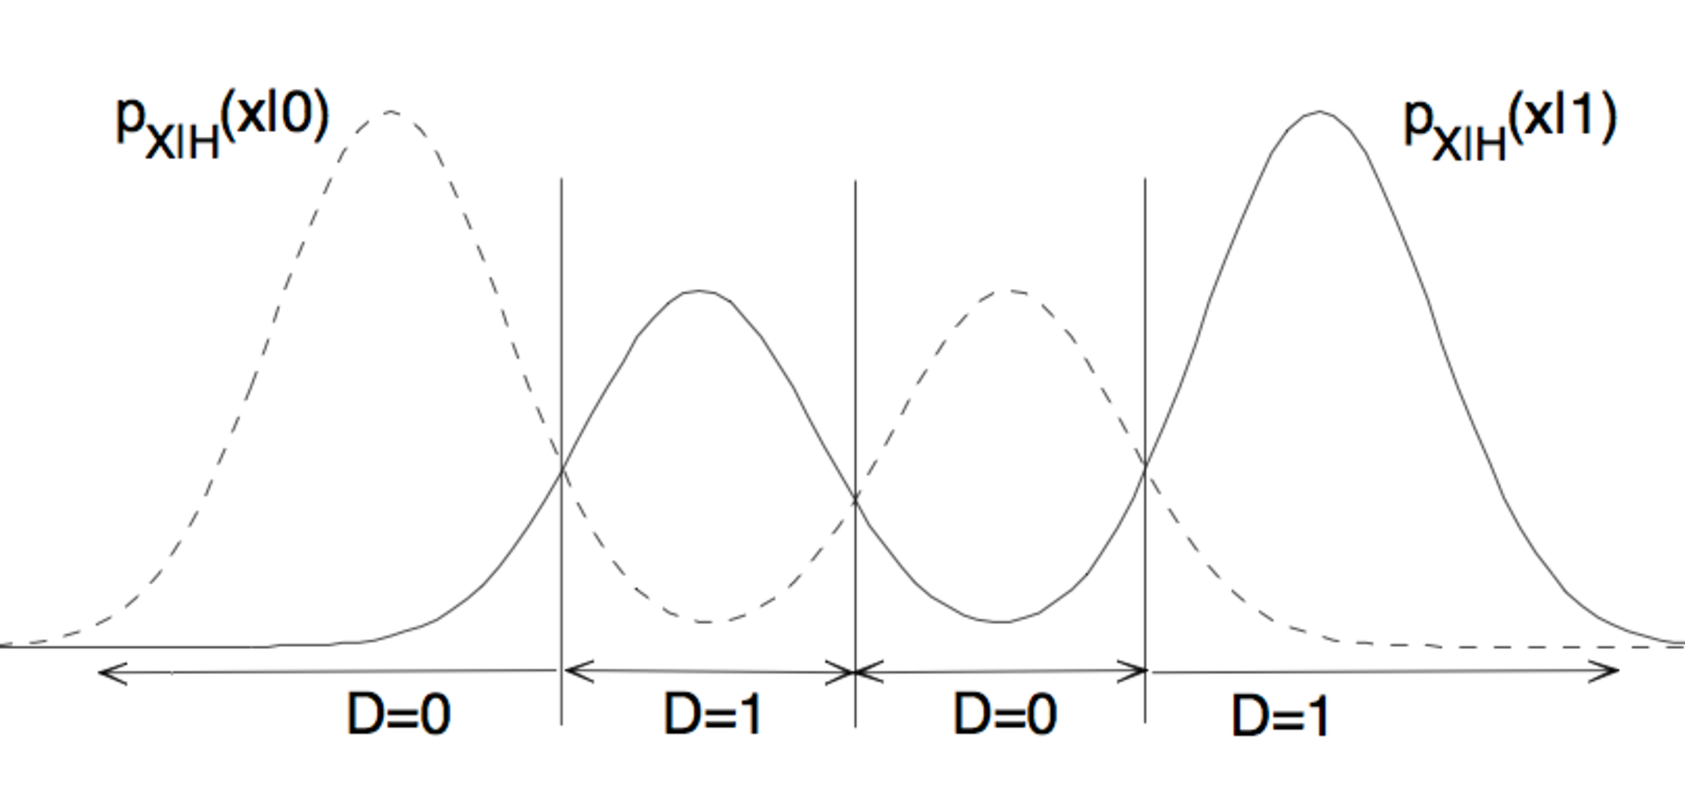
\includegraphics[width=8cm]{Figuras/genera_dist_bimodal.pdf}

\end{parts}
\end{solution}

\else

\question Consider a unidimensional binary decision problem with likelihoods $p_{X|H}(x|h)$ and {\em a priori} probabilities $P_H(h)$, with $h\in \{0,1\}$ and $P_H(1)=0.6$.
\begin{parts}
\part It is known that $P_{H|X}(h|x)=P_{H}(h)$, for $h\in \{0,1\}$, and for all $x$. Determine the MAP classifier.
\part Which is the probability of error of the decision maker obtained in the previous section?
\part Ignore now the condition of section (a). Instead, it is known that the likelihoods are symmetric to each other, i.e.,  $p_{X|H}(x|1)=p_{X|H}(-x|0)$, and that some decision maker given by
\begin{equation}
x \dunodcero \mu  \nonumber
\end{equation}
verifies $P_{FA}=P_{M}$. Which is the value of $\mu$?.
\part Using an equation or a plot, propose and example of symmetric likelihoods (like in the previous section) for which the ML classifier is not a threshold decision maker, i.e., the ML classifier cannot be expressed as
\begin{equation}
x \dunodcero \alpha   \nonumber
\end{equation}
\end{parts}

\begin{solution}
\begin{parts}
\part The MAP classifier always selects $D=1$.
\part $P_{\rm e}=0.4 $
\part $\mu=0$
\part $ $\\
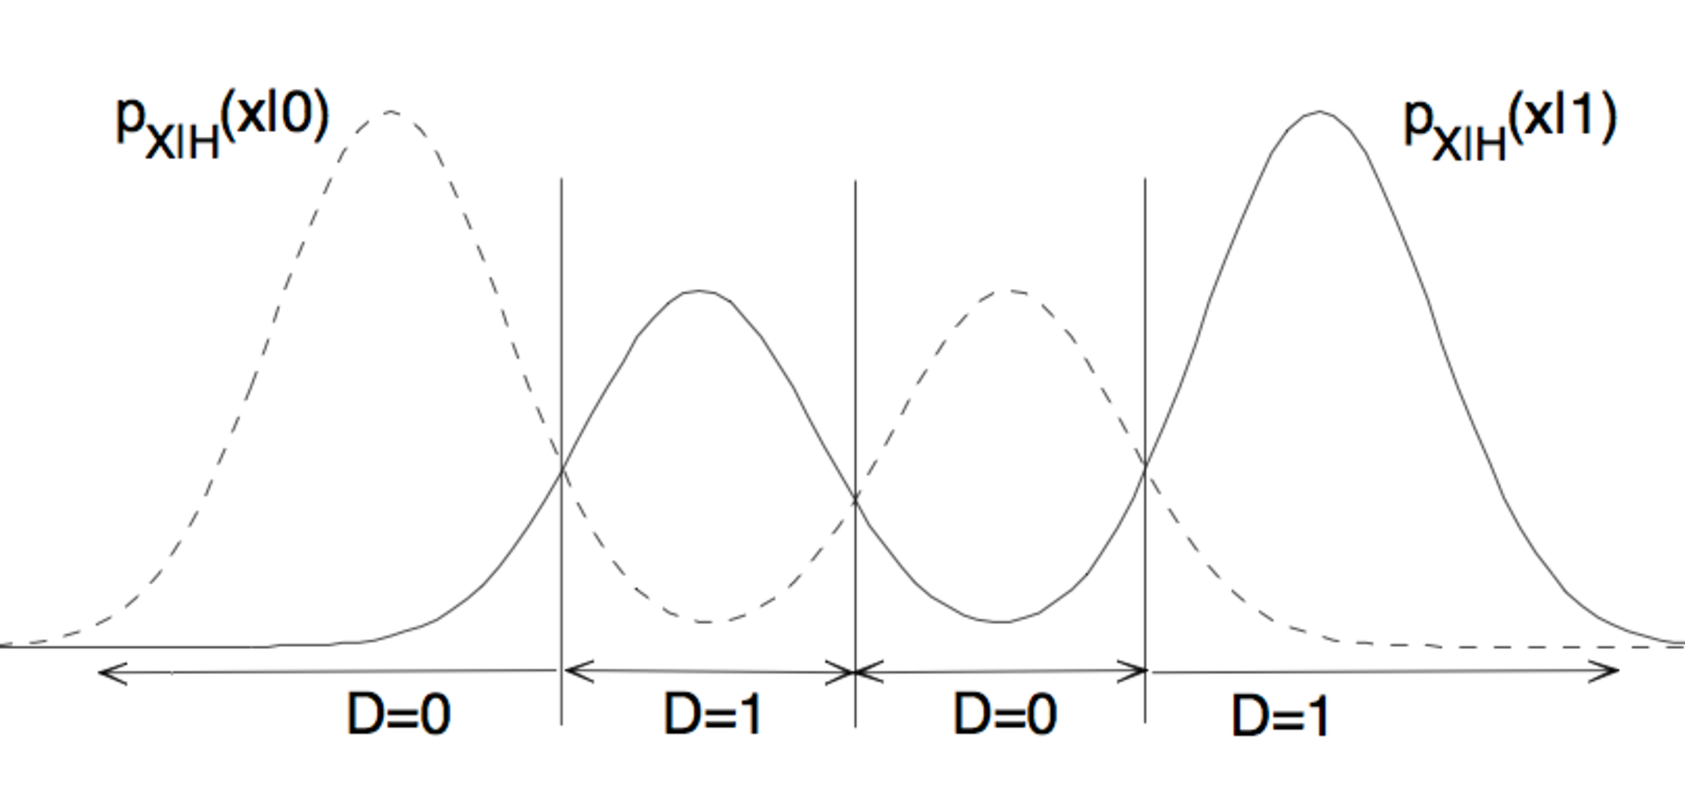
\includegraphics[width=8cm]{Figuras/genera_dist_bimodal.pdf}

\end{parts}
\end{solution}

\fi
%
%%%%%%%%%%%%%%%%%%%%%%%%%%%%%%%%%%%%%%%%%%%%%%%%%%%%%%%%%%%%%%%%%%%%
%% Examen TDI Mayo 2010 P4
\qformat{\textbf{\ej \thequestion ~~ (2.3; 2.4)} ~~ \linefill}
\ifspanish

\question Considere un problema de decisión binaria con hipótesis equiprobables y observaciones caracterizadas por
\begin{equation}
\begin{array}{ll} H=0: & X = N_0 \\ H=1: & X = a + N_1 \end{array}
\nonumber
\end{equation}
siendo $a$ una constante conocida y $N_0$ y $N_1$ variables aleatorias gaussianas con distribuciones $N_0 \sim G(0,v_0)$ y $N_1 \sim G(0,v_1)$, respectivamente.
\begin{parts}
\part Para $a>0$, ilustre gráficamente las regiones de decisión que se obtendrían en los casos $v_0 > v_1$, $v_0 < v_1$ y $v_0 = v_1$.
\part Considere para el resto del ejercicio $a=0$, $v_0 = 1$ y $v_1 = 2$. Obtenga la regla de decisión que minimiza la probabilidad de error del decisor.
\part Obtenga las probabilidades de falsa alarma y de detección que se obtienen al utilizar el decisor anterior. Exprese el resultado haciendo uso de la función $$F(u) = \int_{-\infty}^{u} \frac{1}{\sqrt{2\pi}} \exp\left(-\frac{u^2}{2}\right) du$$
\part Sobre una representación aproximada de la ROC de los decisores tipo LRT
\begin{equation}
\frac{p_{X|H}(x|1)}{p_{X|H}(x|0)} \dunodcero \eta   \nonumber
\end{equation}
indique cómo se desplazaría el punto de trabajo del decisor:
\begin{itemize}
\item al incrementar el umbral $\eta$ del decisor.
\item si crece la probabilidad a priori de la hipótesis $H=1$.
\end{itemize}
\end{parts}

\begin{solution}
\begin{parts}
\part Si $v_0 = v_1$ se obtendría un decisor de único umbral, en caso contrario se obtienen decisores con dos umbrales.
\part $|x| \dunodcero \sqrt{2 \ln 2}=x_u$
\part $\pfa = 2 F(-x_u), \quad \quad \pdet = 2 F\left(\dfrac{-x_u}{\sqrt{2}}\right)$
\part Si $\eta$ crece disminuyen $\pfa$ y $\pdet$. Si $P_H(1)$ crece, manteniendo $\eta$ constante, el punto de trabajo no varía.
\end{parts}
\end{solution}

\else

\question Consider a binary decision problem with equally probable hypotheses and observations characterized by
\begin{equation}
\begin{array}{ll} H=0: & X = N_0 \\ H=1: & X = a + N_1 \end{array}
\nonumber
\end{equation}
where $a$ is a known constant and $N_0$ and $N_1$ are Gaussian random variables with distributions $N_0 \sim G(0,v_0)$ and $N_1 \sim G(0,v_1)$, respectively.
\begin{parts}
\part For $a>0$, provide plots to illustrate the decision regions that would be obtained when $v_0 > v_1$, $v_0 < v_1$, and $v_0 = v_1$.
\part Consider during the rest of the exercise that $a=0$, $v_0 = 1$, and $v_1 = 2$. Obtain the decision rule that minimizes the probability of error of the decider.
\part Calculate the incurred probabilities of false alarm and detection when using the previous decider. Express your results by means of function $$F(z) = \int_{-\infty}^{z} \frac{1}{\sqrt{2\pi}} \exp\left(-\frac{u^2}{2}\right) du$$
\part Using an approximate representation of the ROC of LRT deciders
\begin{equation}
\frac{p_{X|H}(x|1)}{p_{X|H}(x|0)} \dunodcero \eta   \nonumber
\end{equation}
indicate how would the decider operation point move when:
\begin{itemize}
\item threshold $\eta$ is increased.
\item the {\em a priori} probability of hypothesis $H=1$ grows.
\end{itemize}
\end{parts}

\begin{solution}
\begin{parts}
\part If $v_0 = v_1$ we would obtain a classifier based on a single threshold over $x$; otherwise, there would be two thresholds.
\part $|x| \dunodcero \sqrt{2 \ln 2}=x_u$
\part $\pfa = 2 F\left (-x_u\right), \quad  \quad \pdet = 2 F\left ( \dfrac{-x_u}{\sqrt{2}}\right)$
\part If $\eta$ increases, then $\pfa$ and $\pdet$ decrease. If $P_H(1)$ increases with $\eta$ constant, the operation point does not change.
\end{parts}
\end{solution}

\fi
%
%%%%%%%%%%%%%%%%%%%%%%%%%%%%%%%%%%%%%%%%%%%%%%%%%%%%%%%%%%%%%%%%%%%%
%% Examen TDI Junio 2010 P3
\qformat{\textbf{\ej \thequestion ~~ (2.3; 2.6)} ~~ \linefill}
\ifspanish

\question Considere el problema de decisión binaria dado por las verosimilitudes
\begin{align*}
p_{\mathbf X|H}\left( \begin{bmatrix} x_1 \\ x_2 \end{bmatrix} \mid 0\right) 
	&\sim G\left(\begin{bmatrix} 0 \\ 0 \end{bmatrix}, 
	             \begin{bmatrix} 1 & 0 \\ 0 & 1 \end{bmatrix} \right), \\
p_{\mathbf X|H}\left( \begin{bmatrix} x_1 \\ x_2 \end{bmatrix} \mid 1\right) 
    &\sim G\left(\begin{bmatrix} 1 \\ 1 \end{bmatrix}, 
	             \begin{bmatrix} 1 & 0 \\ 0 & 1 \end{bmatrix} \right) 
\end{align*}

\begin{parts}
\part Obtenga la expresión del decisor ML y compruebe que para la toma de la decisión es suficiente conocer la variable $T = X_1 + X_2$.
\part Obtenga las densidades de probabilidad $p_{T|H}(t|0)$ y $p_{T|H}(t|1)$.
\part Calcule las probabilidades de falsa alarma y de pérdida a partir de las verosimilitudes obtenidas en el apartado anterior. Exprese el resultado haciendo uso de la función 
$$F(z)=\int_{-\infty}^z \! \frac{1}{\sqrt{2\pi}}\exp{\left(-\frac{u^2}{2}\right)} \, du $$
\end{parts}

\else

\question Consider a binary decision problem with likelihoods
\begin{align*}
p_{\mathbf X|H}\left( \begin{bmatrix} x_1 \\ x_2 \end{bmatrix} \mid 0\right) 
	&\sim G\left(\begin{bmatrix} 0 \\ 0 \end{bmatrix}, 
	             \begin{bmatrix} 1 & 0 \\ 0 & 1 \end{bmatrix} \right), \\
p_{\mathbf X|H}\left( \begin{bmatrix} x_1 \\ x_2 \end{bmatrix} \mid 1\right) 
    &\sim G\left(\begin{bmatrix} 1 \\ 1 \end{bmatrix}, 
	             \begin{bmatrix} 1 & 0 \\ 0 & 1 \end{bmatrix} \right) 
\end{align*}

\begin{parts}
\part Obtain the ML classifier, and check that the knowledge of $T = X_1 + X_2$ is sufficient for taking decisions.
\part Obtain the conditional probability density functions $p_{T|H}(t|0)$ and $p_{T|H}(t|1)$.
\part Calculate the false alarm and missing probabilities using the likelihoods of the previous section. Express your result by means of function
$$F(z)=\int_{-\infty}^z \! \frac{1}{\sqrt{2\pi}}\exp{\left(-\frac{u^2}{2}\right)} \, du $$
\end{parts}

\fi

%%%%%%%%%%%%%%%%
\begin{solution}
\begin{parts}
\part \ifspanish El clasificador ML está dado por \else The ML classifier is given by \fi
\begin{align*}
p_{{\bf X}|H}({\bf x}\mid 1) & \dunodcero p_{{\bf X}|H}({\bf x}\mid 1)  \\
	\Leftrightarrow \quad & 
		\frac1{2\pi}
	    \exp\left(-\frac12 \left({\bf x}-\begin{bmatrix} 1 \\ 1 \end{bmatrix}\right)^\top  
	                       \left({\bf x}-\begin{bmatrix} 1 \\ 1 \end{bmatrix}\right)\right)
	    \dunodcero
	    \frac1{2\pi}\exp\left(-\frac12 {\bf x}^\top{\bf x}\right) \\ 
	\Leftrightarrow \quad & 
	    - \left({\bf x}-\begin{bmatrix} 1 \\ 1 \end{bmatrix}\right)^\top  
	      \left({\bf x}-\begin{bmatrix} 1 \\ 1 \end{bmatrix}\right) 
		\dunodcero
		- {\bf x}^\top{\bf x}    \\
	\Leftrightarrow \quad & 
	    2 \begin{bmatrix} 1 \\ 1 \end{bmatrix}^\top {\bf x}
	    \dunodcero 
	 	\begin{bmatrix} 1 \\ 1 \end{bmatrix}^\top \begin{bmatrix} 1 \\ 1 \end{bmatrix}    \\
	\Leftrightarrow \quad &  x_1 + x_2 \dunodcero 1 
\end{align*}
\ifspanish Definiendo $t=x_1+x_2$, se obtiene el test equivalente 
\else Defining $t = x_1 + x_2$ we get the equivalent test \fi
\begin{align*}
t \dunodcero 1
\end{align*}

\part 
\ifspanish Dado que $T$ es suma de variables aleatorias gausianas (para cualquier hipótesis), también es gausiana:
\else Since $T$ is a sum of Gaussian random variables (for any hypothesis), it is Gaussian, too: 
\fi
\begin{align*}
p_{T|H}(t|0)\sim G\left (m_0, v_0 \right)   \\
p_{T|H}(t|1)\sim G\left (m_1, v_1 \right)
\end{align*}
\ifspanish donde \else where \fi
\begin{align*}
m_0 &= \EE\{T \mid H=0\} = \EE\{X_1 \mid H=0\} + \EE\{X_2 \mid H=0\} = 0   \\
m_1 &= \EE\{T \mid H=1\} = \EE\{X_1 \mid H=1\} + \EE\{X_2 \mid H=1\} = 2   \\
v_0 &= \EE\{(T-m_0)^2 \mid H=0\} = \EE\{X_1^2 + X_2^2 + 2 X_1 X_2 \mid H=0\} 
     = 1 + 1 + 0 = 2   \\
v_1 &= \EE\{(T-m_1)^2 \mid H=1\} = \EE\{(X_1-1) + (X_2-1))^2 \mid H=1\}  \\
    &= \EE\{(X_1-1)^2 + (X_2-1)^2 + 2 (X_1-1)(X_2-1) \mid H=1\}  = 1+1+0 = 1
\end{align*}
\ifspanish Por tanto, \else Therefore, \fi
\begin{align*}
p_{T|H}(t|0)\sim G\left ( 0, 2 \right)   \\
p_{T|H}(t|1)\sim G\left ( 2, 2 \right)
\end{align*}
\part 
\begin{align*}
\pmis &= \int_{-\infty}^1 p_{T|H}(t \mid 1) dt  
       = \int_{-\infty}^1 \frac1{\sqrt{4 \pi}} \exp\left(-\frac14 (t-2)^2 \right) dt  \\
      &= \int_{-\infty}^\frac1{\sqrt{2}} \frac1{\sqrt{2 \pi}} \exp\left(-\frac14 z^2 \right) dz
       = F\left (-\frac1{\sqrt{2}}\right)   \\
\pfa  &= \int_1^\infty p_{T|H}(t \mid 0) dt 
       = \int_1^\infty \frac1{\sqrt{4 \pi}} \exp\left(-\frac14 t^2 \right) dt   \\
      &= \int_{\frac1{\sqrt{2}}}^\infty \frac1{\sqrt{2 \pi}} \exp\left(-\frac12 t^2 \right) dt
       = 1 - F\left (\frac1{\sqrt{2}}\right)
\end{align*}
\ifspanish Nótese que, siendo $F(-z)=1-F(z)$, para todo $z \in \mathbb{R}$, resulta $\pfa=\pmis$.
\else Note that, since $F(-z)=1-F(z)$, for any $z \in \mathbb{R}$, we have $\pfa=\pmis$.
\fi
\end{parts}
\end{solution}
%%%%%%%%%%%%%%

%
%%%%%%%%%%%%%%%%%%%%%%%%%%%%%%%%%%%%%%%%%%%%%%%%%%%%%%%%%%%%%%%%%%%%
%% Examen TDI Junio 2010 P5
\qformat{\textbf{\ej \thequestion ~~ (2.2; 2.4 ; 2.5)} ~~ \linefill}
\ifspanish

\question Se tiene un problema de clasificación binaria definido por las siguientes verosimilitudes:
$$p_{X|H}(x|0) = 2 \exp\left(-2x \right) \quad x>0$$
$$p_{X|H}(x|1) =1 \quad 0<x<1 $$ 
\begin{parts}
\part Obtenga el test de razón de verosimilitudes para un valor genérico del umbral $\eta$
$$\frac{p_{X|H}(x|1)}{p_{X|H}(x|0)} \dunodcero \eta$$
\part Calcule la probabilidad de falsa alarma y de pérdidas del decisor anterior en función de $\eta$
\part Represente la curva característica de operación del decisor e indique sobre la misma los puntos de trabajo de:
\begin{itemize}
\item El decisor de máxima verosimilitud
\item El decisor máximo a posteriori si $P_H(0)=2P_H(1)$
\item El decisor Neyman Pearson para $P_{FA}\leq 0.1$
\end{itemize}
\part Considere ahora el siguiente decisor de umbral sobre la observación $x$
$$x \dunodcero \eta_u$$

y obtenga su probabilidad de falsa alarma y de pérdidas en función de $\eta_u$
\part Represente la curva característica de operación del decisor de umbral anterior y compárela con la curva característica del decisor LRT. ¿Qué esquema de decisión (el obtenido mediante el LRT o mediante un test de umbral) presenta mejores prestaciones? Justifique su respuesta.
\end{parts}

\begin{solution}
\begin{parts}
\part $\left\lbrace  \begin{array}{ll} 
D=1: & \eta' < x < 1 \\
D=0: & 0 < x < \eta'  \quad {\rm y} \quad x>1 
\end{array} \right. $ \\
donde $\displaystyle \eta'=\frac{1}{2} \ln 2 \eta$ y $\eta'>0$
\part $\displaystyle P_{\rm FA}=\left\lbrace \begin{array}{ll} \exp(-2\eta') -\exp(-2) &   0<\eta'<1 \\ 0 &  \eta'>1 \end{array} \quad \right.  \quad P_{\rm M}=\left\lbrace \begin{array}{ll} \eta' &  0<\eta'<1 \\ 1 &  \eta'>1 \end{array} \right. $
\part $ $ \\
\begin{tabular}{ll}
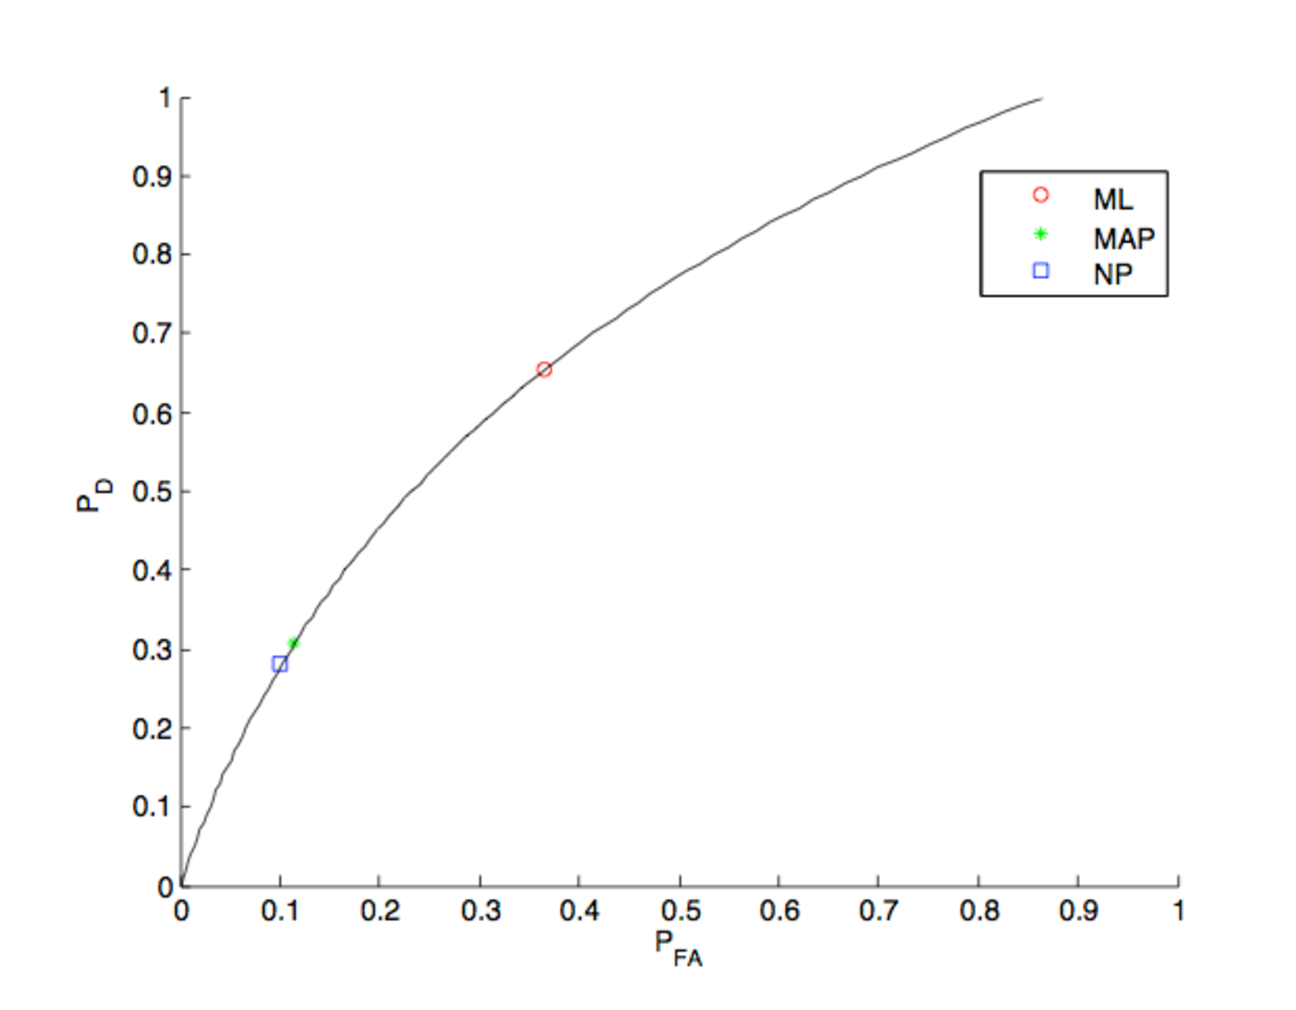
\includegraphics[width=5cm]{Figuras/ROC_jun2010_a.pdf} & 
$ \displaystyle  \begin{array}{lll} {\rm ML:}&  P_{\rm FA}= \frac{1}{2} -\exp(-2)  &  P_D=1-\frac{1}{2} \ln2 \\  {\rm MAP:}&  P_{\rm FA}= \frac{1}{4} -\exp(-2)  &  P_D=1- \ln2 \\ 
 {\rm N-P:}&  P_{\rm FA}= 0.1  \end{array} $
\end{tabular}
\part 
$\displaystyle P_{\rm FA}=\exp(-2\eta_u)\quad  \quad P_{\rm M}=\left\lbrace \begin{array}{ll} \eta_u&  0<\eta_u<1 \\ 1 &  \eta_u>1 \end{array} \right. $

\part $ $ \\
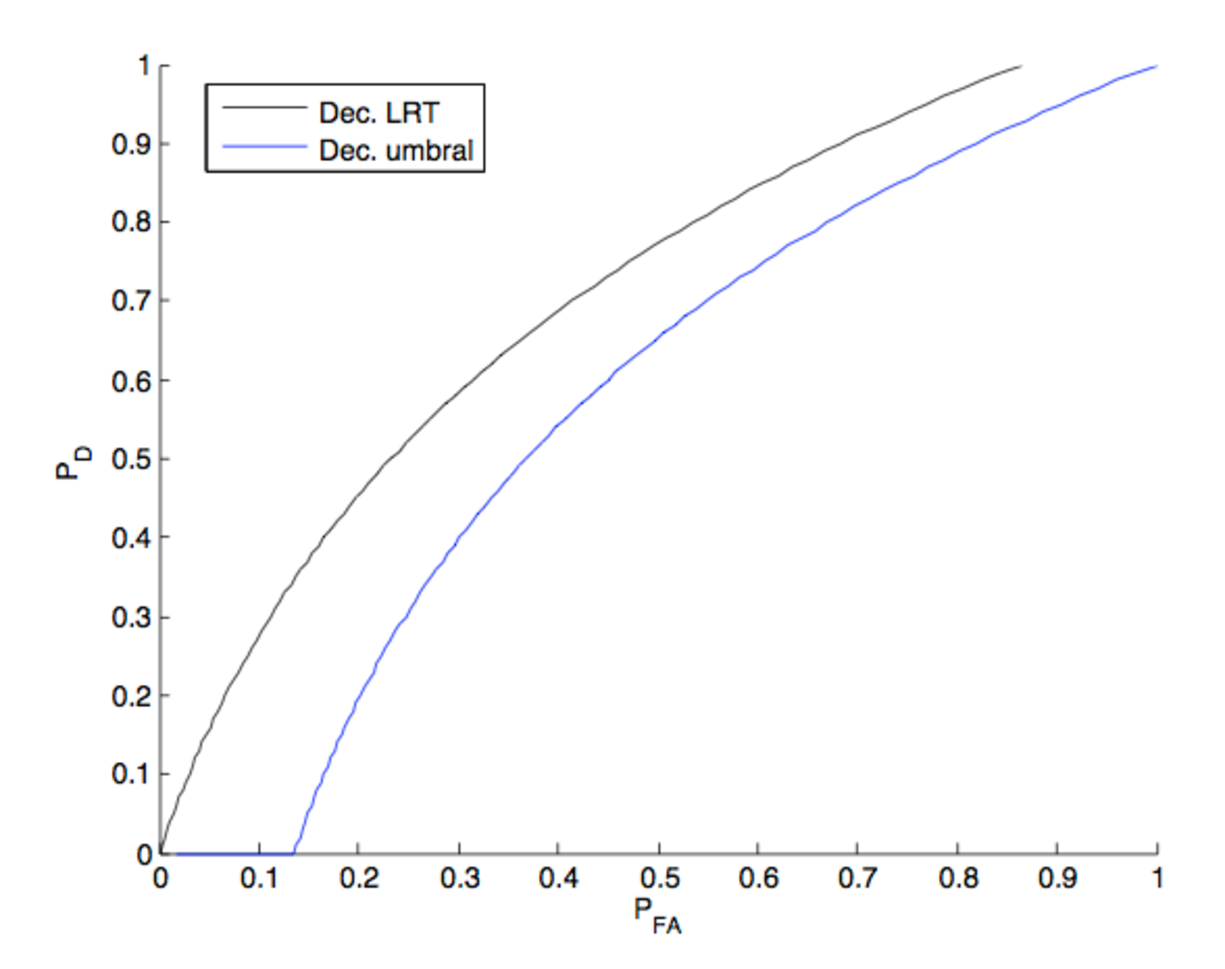
\includegraphics[width=5cm]{Figuras/ROC_jun2010_b.pdf}\\
Como era de esperar la curva ROC del decisor LRT está por encima de la ROC del decisor de umbral, por lo que confirmamos que el decisor LRT presenta mejores prestaciones.
\end{parts}

\end{solution}

\else

\question Consider a binary decision problem characterized by the following likelihoods:
$$p_{X|H}(x|0) = 2 \exp\left(-2x \right) \quad x>0$$
$$p_{X|H}(x|1) =1 \quad 0<x<1 $$ 
\begin{parts}
\part Obtain the likelihood ratio test for a generic value of threshold $\eta$.
$$\frac{p_{X|H}(x|1)}{p_{X|H}(x|0)} \begin{array}{c} {\scriptsize{D=1}} \\ \gtrless \\ {\scriptsize{D=0}}\end{array} \eta$$
\part Calculate the false alarm and missing probabilities of the previous decision maker as a function of $\eta$.
\part Plot the operating characteristic curve (ROC) of the decision maker, indicating in your representation the operation points of:
\begin{itemize}
\item The maximum likelihood decision maker
\item The maximum {\em a posteriori} decision maker, for $P_H(0)=2P_H(1)$
\item The Neyman-Pearson detector with $P_{FA}\leq 0.1$
\end{itemize}
\part Consider now a second decision maker consisting on imposing a threshold on the observation $x$
$$x \begin{array}{c} {\scriptsize{D=1}} \\ \gtrless \\ {\scriptsize{D=0}}\end{array} \eta_u$$
Obtain the false alarm and missing probabilities of this classifier as a function of $\eta_u$.
\part Plot the ROC of the new decision maker, and compare it with the ROC of the LRT decision maker. Which decision scheme (the one based on the LRT or the one based on a threshold over $x$) offers a better performance? Justify your answer.
\end{parts}

\begin{solution}
\begin{parts}
\part $\left\lbrace  \begin{array}{ll} 
D=1: & \eta' < x < 1 \\
D=0: & 0 < x < \eta'  \quad {\rm and} \quad x>1 
\end{array} \right. $ \\
where $\displaystyle \eta'=\frac{1}{2} \ln 2 \eta$ and $\eta'>0$
\part $\displaystyle P_{\rm FA}=\left\lbrace \begin{array}{ll} \exp(-2\eta') -\exp(-2) &   0<\eta'<1 \\ 0 &  \eta'>1 \end{array} \quad \right.  \quad P_{\rm M}=\left\lbrace \begin{array}{ll} \eta' &  0<\eta'<1 \\ 1 &  \eta'>1 \end{array} \right. $
\part $ $ \\
\begin{tabular}{ll}
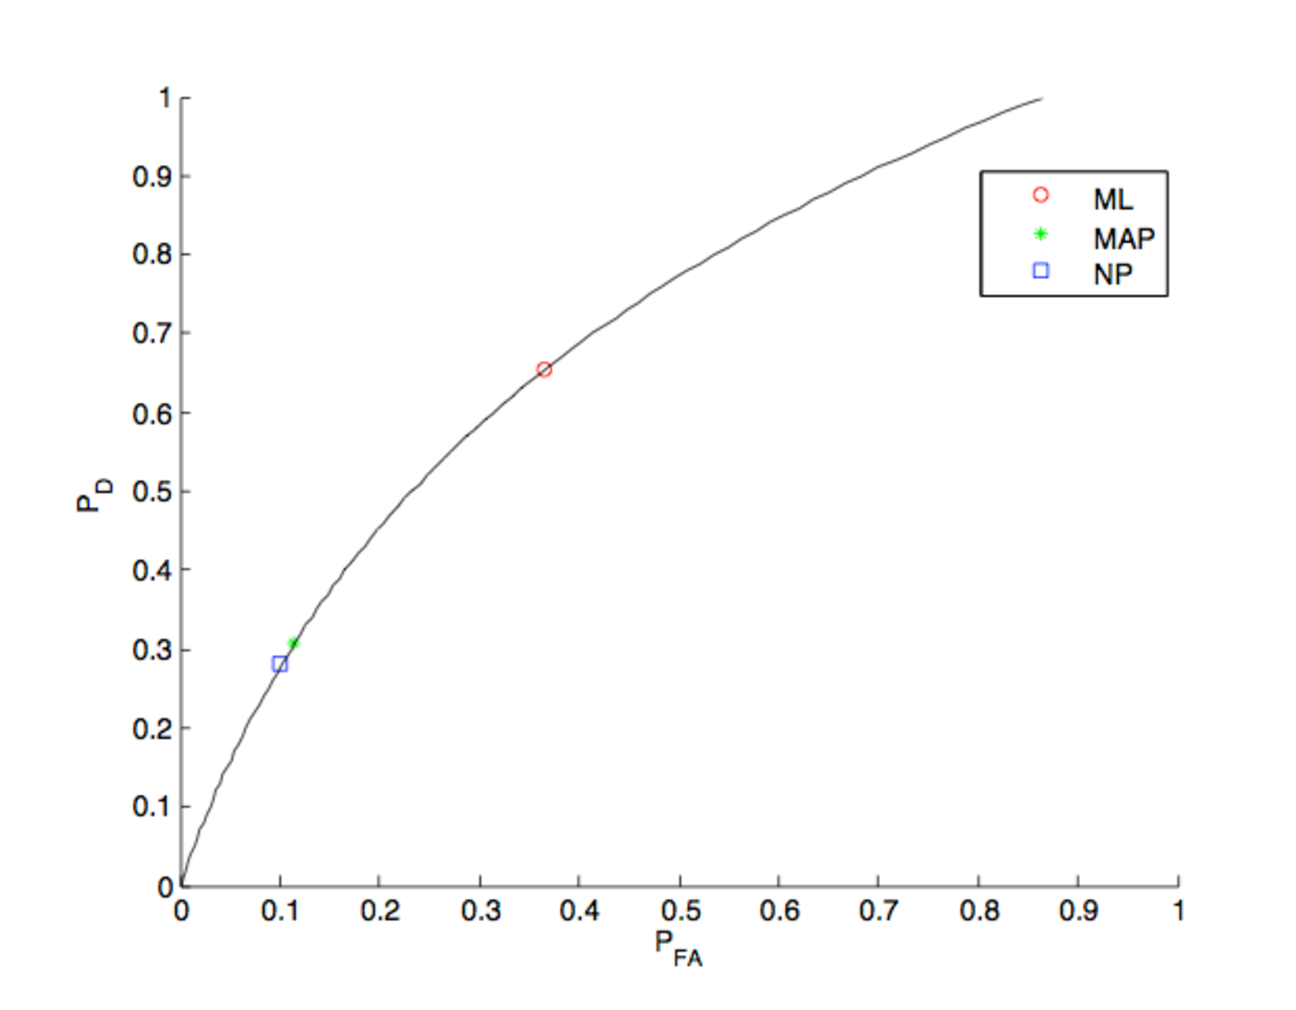
\includegraphics[width=5cm]{Figuras/ROC_jun2010_a.pdf} & 
$ \displaystyle  \begin{array}{lll} {\rm ML:}&  P_{\rm FA}= \frac{1}{2} -\exp(-2)  &  P_D=1-\frac{1}{2} \ln2 \\  {\rm MAP:}&  P_{\rm FA}= \frac{1}{4} -\exp(-2)  &  P_D=1- \ln2 \\ 
 {\rm N-P:}&  P_{\rm FA}= 0.1  \end{array} $
\end{tabular}
\part 
$\displaystyle P_{\rm FA}=\exp(-2\eta_u)\quad  \quad P_{\rm M}=\left\lbrace \begin{array}{ll} \eta_u&  0<\eta_u<1 \\ 1 &  \eta_u>1 \end{array} \right. $

\part $ $ \\
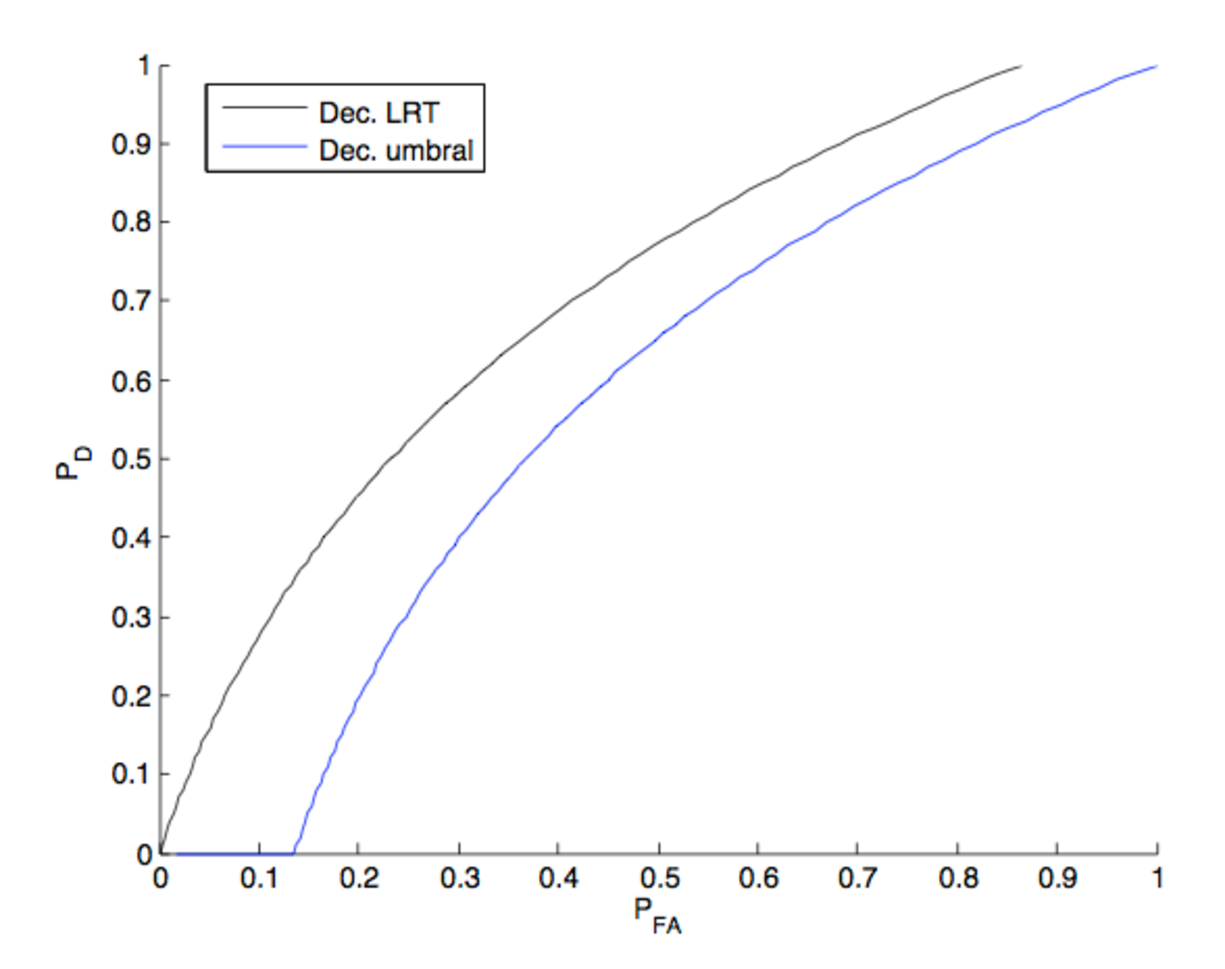
\includegraphics[width=5cm]{Figuras/ROC_jun2010_b.pdf}\\
As expected, the ROC corresponding to the LRT is above the ROC of the based on thresholding $x$; we confirm that the LRT decision makers achieve better performance.
\end{parts}

\end{solution}

\fi

%%%%%%%%%%%%%%%%%%%%%%%%%%%%%%%%%%%%%%%%%%%%%%%%%%%%%%%%%%%%%%%%%%%%
%% Examen TDI Mayo 2011 P2
\qformat{\textbf{\ej \thequestion ~~ (2.2; 2.5)} ~~ \linefill}
\ifspanish

\question Considere el problema de decisión binaria dado por las verosimilitudes
\[
p_{X|H}(x|0) = n (1-x)^{n-1},  \qquad  0 \le x \le 1
\]
\[
p_{X|H}(x|1) = n x^{n-1},  \qquad  0 \le x \le 1
\]
siendo $n\ge 2$ un número natural.
\begin{parts}
\part Determine las regiones de decisión de un decisor LRT, en función de su umbral, $\eta$.
\part Determine, en función de $n$ y $\eta$, las probabilidades de falsa alarma y pérdida.
\part Determine el decisor minimax.
\end{parts}


\begin{solution}
\begin{parts}
\part $\displaystyle x \dunodcero \frac{\eta^{\frac{1}{n-1}}}{1+\eta^{\frac{1}{n-1}}} $ \\
\part $P_{\rm FA} =\left( \frac{1}{1+\eta^{\frac{1}{n-1}} }\right)^n $\\
$P_{\rm M} =\left( \frac{\eta^{\frac{1}{n-1}}}{1+\eta^{\frac{1}{n-1}} }\right)^n $
\part  $\displaystyle x \dunodcero \frac{1}{2} $
\end{parts}
\end{solution}

\else

\question Consider a binary decision problem characterized by the following likelihoods
\[
p_{X|H}(x|0) = n (1-x)^{n-1},  \qquad  0 \le x \le 1
\]
\[
p_{X|H}(x|1) = n x^{n-1},  \qquad  0 \le x \le 1
\]
with $n\ge 2$ a natural number.
\begin{parts}
\part Determine the decision regions of an LRT decider, as a function of the threshold of the test, $\eta$.
\part Obtain, as a function of $n$ and $\eta$, the false alarm and missing probabilities.
\part Determine the minimax decider.
\end{parts}

\begin{solution}
\begin{parts}
\part $\displaystyle x \dunodcero \frac{\eta^{\frac{1}{n-1}}}{1+\eta^{\frac{1}{n-1}}} $ \\
\part $P_{\rm FA} =\left( \frac{1}{1+\eta^{\frac{1}{n-1}} }\right)^n $\\
$P_{\rm M} =\left( \frac{\eta^{\frac{1}{n-1}}}{1+\eta^{\frac{1}{n-1}} }\right)^n $
\part  $\displaystyle x \dunodcero \frac{1}{2} $
\end{parts}
\end{solution}

\fi
%
%%%%%%%%%%%%%%%%%%%%%%%%%%%%%%%%%%%%%%%%%%%%%%%%%%%%%%%%%%%%%%%%%%%%
%% Examen TDI Mayo 2011 P4
\qformat{\textbf{\ej \thequestion ~~ (2.2)} ~~ \linefill}
\ifspanish

\question Considere un problema de clasificación binaria caracterizado por $P_H(0) = P_H(1) = 1/2$, $c_{00} = c_{11} = 0$, $c_{01} = 9$, $c_{10} = 8$, y verosimilitudes
$$p_{X|H}(x|0) = 1-\frac{x}{2}; \quad\quad 0 \leq x \leq 2$$
$$p_{X|H}(x|1) = \frac{2}{3}; \quad\quad 0 \leq x \leq 3/2$$

\begin{parts}
\part Considere un clasificador LRT genérico:
$$\frac{p_{X|H}(x|0)}{p_{X|H}(x|1)} \dceroduno \eta$$
 Muestre gráficamente las regiones de decisión de dicho clasificador en el intervalo $x \in [0,2]$, indicando cómo varían dichas regiones con $\eta$.

\part Calcule $P_\text{FA}$ y $P_\text{D}$ para el clasificador LRT, expresándolas como función de $\eta$.

\part Diseñe el clasificador ML, y calcule sus $P_\text{FA}$ y $P_\text{M}$.%, y el coste medio incurrido por dicho clasificador.
\part Considere ahora el siguiente clasificador de umbral genérico:
$$x \dunodcero \eta'$$
Obtenga, en función de $\eta'$, los valores de $P_\text{FA}$ y $P_\text{D}$.  Rellene la siguiente tabla particularizando las expresiones obtenidas para los valores indicados del umbral.

\begin{center}
\begin{tabular}{|c|c|c|c|c|c|}
\hline
$\eta'$ & ~~~0~~~ & ~~0.5~~ & ~~~1~~~  & ~~1.5~~   & ~~~2~~~ \\ \hline
$P_\text{FA}$ & & & & & \\ \hline
$P_\text{D}$ & & & & & \\ \hline
\end{tabular}
\end{center}


%\part Represente, de manera aproximada, la ROC ($P_\text{D}$ {\em{vs}} $P_\text{FA}$) que caracteriza al clasificador de umbral. JUSTIFIQUE si esta ROC está por encima o por debajo de la curva ROC correspondiente al LRT del apartado (a).

\part Proporcione, en función del valor de $\eta'$, la expresión del coste medio para la familia de clasificadores de umbral considerada en el apartado anterior. Encuentre el valor de $\eta'$ que minimiza dicho coste medio.
\end{parts}


\begin{solution}
\begin{parts}
\part Si $x>\frac{3}{2}$ siempre se decide $D=0$. Si $x>\frac{3}{2}$ el decisor LRT queda:\\
$$x \dunodcero 2-\frac{4\eta}{3}=\mu$$
Que indica:
\begin{itemize}
\item Si $\eta>\frac{3}{2}$ ($\mu<0$) siempre se decide $D=1$.
\item Si $\eta<\frac{3}{8}$ ($\mu>\frac{3}{2}$) siempre se decide $D=0$.
\item Si $\frac{3}{2}<\eta<\frac{3}{8}$, se decide $D=0$ si $0<x<\mu$ y $D=1$ si $\mu<x<\frac{3}{2}$ 
\end{itemize}

\part 
\begin{itemize}
\item Si $\eta>\frac{3}{2}$ ($\mu<0$), $\pfa = \pdet = 1$.
\item Si $\eta<\frac{3}{8}$ ($\mu>\frac{3}{2}$), $\pfa = \pdet = 0$.
\item Si $\frac{3}{2}<\eta<\frac{3}{8}$, $\pfa = \dfrac{15}{16} - \mu + \dfrac{\mu^2}{4}$, $\pdet =1-\dfrac{2\mu}{3}$
\end{itemize}
\part Decisor ML ($\eta=1$ y $\mu=\frac{2}{3}$):  $\pmis =\dfrac{4}{9}$ y  $\pfa = \dfrac{55}{144}$
\part Si $0<\eta'<\frac{3}{2}$: $P_{\rm FA} =1-\eta'+\dfrac{\eta'^2}{4}$ y $P_{\rm D} =1-\dfrac{2\eta'}{3}$ \\
Si $\frac{3}{2}<\eta'<2$: $P_{\rm FA} =1-\eta'+\dfrac{\eta'^2}{4}$ y $P_{\rm D}=0$ \\

\begin{center}
\begin{tabular}{|c|c|c|c|c|c|}
\hline
$\eta'$ & ~~~0~~~ & ~~0.5~~ & ~~~1~~~  & ~~1.5~~   & ~~~2~~~ \\ \hline
$P_\text{FA}$ & $1$ & $\frac{9}{16}$ &$\frac{1}{4}$  & $\frac{1}{16}$ & $0$\\ \hline
$P_\text{D}$ &$ 1$ & $\frac{2}{3}$& $\frac{1}{3}$& $0$ & $0$ \\ \hline
\end{tabular}
\end{center}

\part $\displaystyle \mathbb{E} \left\lbrace c_{DH} \right\rbrace = \left[  \eta'-2 \right]^2 +3\eta'$, si $\displaystyle 0<\eta'<\frac{3}{2}$\\
 $\displaystyle \mathbb{E} \left\lbrace c_{DH} \right\rbrace = \left[  \eta'-2 \right]^2 +\frac{9}{2}$, si $\displaystyle \eta'>\frac{3}{2}$\\
$\displaystyle \eta'^*=\frac{1}{2}$

\end{parts}
\end{solution}

\else

\question Consider a binary classification problem characterized by $P_H(0) = P_H(1) = 1/2$, $c_{00} = c_{11} = 0$, $c_{01} = 9$, $c_{10} = 8$, and likelihoods
$$p_{X|H}(x|0) = 1-\frac{x}{2}; \quad\quad 0 \leq x \leq 2$$
$$p_{X|H}(x|1) = \frac{2}{3}; \quad\quad 0 \leq x \leq 3/2$$

\begin{parts}

%\part Design the ML classifier for such situation, and calculate $P_\text{FA}$, $P_\text{M}$, and the risk incurred by such classifier.

\part Consider a generic LRT classifier:
$$\frac{p_{X|H}(x|0)}{p_{X|H}(x|1)} \dceroduno \eta$$
Illustrate the decision regions of such a classifier for interval $x \in [0,2]$, explaining how these regions change when modifying the threshold of the test.

\part Obtain $P_\text{FA}$ and $P_\text{D}$ for the LRT classifier, expressing them as a function of $\eta$.

\part Design the ML classifier for the problem under consideration, and obtain its $P_\text{FA}$ and $P_\text{M}$.

\part Consider now the following threshold classifier:
$$x \dunodcero \eta'$$
Obtain, as a function of $\eta'$, the values of $P_\text{FA}$ and $P_\text{D}$.  Fill in the following table particularizing your expressions for the indicated values of the threshold.
\begin{table}[h]
\begin{center}
\begin{tabular}{|c|c|c|c|c|c|}
\hline
$\eta'$ & ~~~0~~~ & ~~0.5~~ & ~~~1~~~  & ~~1.5~~   & ~~~2~~~ \\ \hline
$P_\text{FA}$ & & & & & \\ \hline
$P_\text{D}$ & & & & & \\ \hline
\end{tabular}
\end{center}
\end{table}

%\part Plot, in an approximate manner, the ROC ($P_\text{D}$ {\em{vs}} $P_\text{FA}$) of the threshold classifier.   JUSTIFY if this ROC is above or below that characterizing the LRT of section (b).

\part Provide, as a function of $\eta'$, an expression for the risk of the threshold classifier considered in the previous subsection. Find the value of $\eta'$ that minimizes such risk.

\end{parts}

\begin{solution}
\begin{parts}
\part If $x>\frac{3}{2}$ the classifier always decides $D=0$. If $x>\frac{3}{2}$ the LRT classifier is:\\
$$x \dunodcero 2-\frac{4\eta}{3}=\mu$$
So we can find the following situations:
\begin{itemize}
\item If $\eta>\frac{3}{2}$ ($\mu<0$) it always decides $D=1$.
\item If $\eta<\frac{3}{8}$ ($\mu>\frac{3}{2}$) it always decides $D=0$.
\item If $\frac{3}{2}<\eta<\frac{3}{8}$, the classifier decides $D=0$ for $0<x<\mu$ and $D=1$ for $\mu<x<\frac{3}{2}$ 
\end{itemize}

\part 
\begin{itemize}
\item If $\eta>\frac{3}{2}$ ($\mu<0$), $\pfa = \pdet = 1$.
\item If $\eta<\frac{3}{8}$ ($\mu>\frac{3}{2}$), $\pfa = \pdet = 0$.
\item If $\frac{3}{2}<\eta<\frac{3}{8}$, $\pfa = \dfrac{15}{16} - \mu + \dfrac{\mu^2}{4}$, $\pdet =1-\dfrac{2\mu}{3}$
\end{itemize}
\part ML Decider ($\eta=1$ and $\mu=\dfrac{2}{3}$):  $\pmis =\dfrac{4}{9}$ and  $\pfa =\dfrac{55}{144}$
\part If $0<\eta'<\frac{3}{2}$: $\pfa =1-\eta'+\dfrac{\eta'^2}{4}$ and $\pdet =1-\dfrac{2\eta'}{3}$\\
If $\frac{3}{2}<\eta'<2$:  $\pfa = 1-\eta'+\dfrac{\eta'^2}{4}$ and $\pdet = 0$
\begin{center}
\begin{tabular}{|c|c|c|c|c|c|}
\hline
$\eta'$ & ~~~0~~~ & ~~0.5~~ & ~~~1~~~  & ~~1.5~~   & ~~~2~~~ \\ \hline
$P_\text{FA}$ & $1$ & $\frac{9}{16}$ &$\frac{1}{4}$  & $\frac{1}{16}$ & $0$\\ \hline
$P_\text{D}$ &$ 1$ & $\frac{2}{3}$& $\frac{1}{3}$& $0$ & $0$ \\ \hline
\end{tabular}
\end{center}


\part $\displaystyle \mathbb{E} \left\lbrace c_{DH} \right\rbrace = \left[  \eta'-2 \right]^2 +3\eta'$, if $\displaystyle 0<\eta'<\frac{3}{2}$\\
 $\displaystyle \mathbb{E} \left\lbrace c_{DH} \right\rbrace = \left[  \eta'-2 \right]^2 +\frac{9}{2}$, if $\displaystyle \eta'>\frac{3}{2}$\\
$\displaystyle \eta'^*=\frac{1}{2}$

\end{parts}
\end{solution}

\fi
%
%%%%%%%%%%%%%%%%%%%%%%%%%%%%%%%%%%%%%%%%%%%%%%%%%%%%%%%%%%%%%%%%%%%%
%% Examen TDI Junio 2011 P3
\qformat{\textbf{\ej \thequestion ~~ (2.3; 2.6)} ~~ \linefill}
\ifspanish

\question Se tiene un problema de decisión binaria definido por las siguientes verosimilitudes:
\begin{align*}
p_{X_1,X_2|H}(x_1,x_2 \mid 0)
	&= G\left(\begin{bmatrix} -1 \\ 0 \end{bmatrix}, 
	          \begin{bmatrix} 1 & \rho \\ \rho & 1 \end{bmatrix} \right)  \\
p_{X_1,X_2|H}(x_1,x_2 \mid 1) 
	&= G\left(\begin{bmatrix} 1 \\ 0 \end{bmatrix}, 
	         \begin{bmatrix} 1 & \rho \\ \rho & 1	 \end{bmatrix} \right) 
\end{align*}
siendo $|\rho |<1$.
\begin{parts}
\part Obtenga el decisor de máxima verosimilitud. 
\part Considere la v.a. $Z= X_1-\rho X_2$ y obtenga las verosimilitudes de $H=0$ y $H=1$ sobre dicha v.a., $p_{Z|H}(z|0)$ y $p_{Z|H}(z|1)$.
\part Considerando los resultados de los apartados anteriores, calcule las probabilidades de falsa alarma y de pérdida del decisor dise\~nado en (a); exprese estas probabilidades utilizando la función
$$F(x) = 1- Q(x) = \int_{-\infty}^x \frac{1}{\sqrt{2\pi}} \exp{\left( - \frac{t^2}{2}\right) } \; dt$$
\end{parts}

\begin{solution}
\begin{parts}
\part $ X_1-\rho X_2 \dunodcero 0$
\part $ p_{Z|H}(z | 0) = G \left(-1, 1-\rho^2 \right) $ \hspace{1cm}
 $ p_{Z|H}(z | 1) = G \left(1, 1-\rho^2 \right) $ 
 \part $\displaystyle  P_{\rm FA} =P_{\rm M} =F\left(-\frac{1}{\sqrt{1-\rho^2}} \right) $
\end{parts}

\end{solution}

\else

\question A binary decision problem is characterized by Gaussian likelihoods:
\begin{align*}
p_{X_1,X_2|H}(x_1,x_2 \mid 0)
	&= G\left(\begin{bmatrix} -1 \\ 0 \end{bmatrix}, 
	          \begin{bmatrix} 1 & \rho \\ \rho & 1 \end{bmatrix} \right)  \\
p_{X_1,X_2|H}(x_1,x_2 \mid 1) 
	&= G\left(\begin{bmatrix} 1 \\ 0 \end{bmatrix}, 
	         \begin{bmatrix} 1 & \rho \\ \rho & 1	 \end{bmatrix} \right) 
\end{align*}
where $|\rho |<1$.
\begin{parts}
\part Design the maximum likelihood decision maker. 
\part Let $Z= X_1-\rho X_2$ be a new random variable. Obtain the likelihoods of hypotheses $H=0$ and $H=1$ in terms of the new random variable, $p_{Z|H}(z|0)$ and $p_{Z|H}(z|1)$.
\part Considering the results of the previous sections, calculate the False Alarm and Missing probabilities of the decision maker designed in Section (a); express your results in terms of function
$$F(x) = 1- Q(x) = \int_{-\infty}^x \frac{1}{\sqrt{2\pi}} \exp{\left( - \frac{t^2}{2}\right) } \; dt$$
\end{parts}

\begin{solution}
\begin{parts}
\part $ X_1-\rho X_2 \dunodcero 0$
\part $ p_{Z|H}(z | 0) = G \left(-1, 1-\rho^2 \right) $ \hspace{1cm}
 $ p_{Z|H}(z | 1) = G \left(1, 1-\rho^2 \right) $ 
 \part $\displaystyle  P_{\rm FA} =P_{\rm M} =F\left(-\frac{1}{\sqrt{1-\rho^2}} \right) $
\end{parts}

\end{solution}

\fi
%
%%%%%%%%%%%%%%%%%%%%%%%%%%%%%%%%%%%%%%%%%%%%%%%%%%%%%%%%%%%%%%%%%%%%
%% Examen TDI Junio 2011 P3
\qformat{\textbf{\ej \thequestion ~~ (2.1; 2.2; 2.5)} ~~ \linefill}
\ifspanish

\question
Considere un problema de decisión binaria con hipótesis equiprobables basado en la observación de una variable aleatoria $X$, con verosimilitudes.
\[
p_{X|H}(x|0) = \left \{
  \begin{array}{cc}
    1, & 0 \le x \le 1\\
0, & \mbox{en el resto}
  \end{array}
\right.
\]
\[
p_{X|H}(x|1) = \left \{
  \begin{array}{cc}
    2x, & 0 \le x \le 1\\
0, & \mbox{en el resto}
  \end{array}
\right.
\]

\begin{parts}
 \part Calcule la probabilidad de error del decisor MAP.
 \part Determine el decisor Neyman-Pearson de probabilidad de falsa alarma $P_\text{FA} \le 1/4$.
 \part Ahora suponga que la variable aleatoria hipótesis puede tomar un tercer valor $H=2$, con verosimilitud
\[
p_{X|H}(x|2) = \left \{
  \begin{array}{cc}
    2(1-x), & 0 \le x \le 1\\
0, & \mbox{en el resto}
  \end{array}
\right.
\]

Para el caso de que las 3 hipótesis sean equiprobables y se aplique una política de costes
\[
c_{00} = c_{11} = c_{22}=0, c_{02} = c_{10} = c_{12}= c_{20}=1, c_{01}=c_{21}=2
\]
donde $c_{dh}$ es el coste de decidir $D=d$ cuando la hipótesis
correcta es $H=h$, calcule el coste medio de tomar cada decisión a la
vista de $X$, es decir, calcule
\[
\mathbb E\{c_{0,H}|x\}, \; \mathbb E\{c_{1,H}|x\}  \mbox{ y } \mathbb E\{c_{2,H}|x\} 
\]

\part Represente los costes medios calculados en el apartado anterior
como funciones de la observación $x$ y determine las regiones del
decisor de mínimo coste medio.
\end{parts}


\begin{solution}
\begin{parts}
 \part $\displaystyle  P_{\rm e} =\frac{3}{8} $
  \part $\displaystyle  x \dunodcero \frac{3}{4} $
\part $\displaystyle  \mathbb E\{c_{0,H}|x\}  = \frac{2}{3}x+\frac{2}{3}$ \hspace{0.5cm}
  $\displaystyle  \mathbb E\{c_{1,H}|x\}  =1- \frac{2}{3}x$ \hspace{0.5cm}
  $\displaystyle  \mathbb E\{c_{2,H}|x\}  = \frac{4}{3}x+\frac{1}{3}$
  \part  $ \left \{
  \begin{array}{cc}
    D=2 & 0 \le x \le \displaystyle  \frac{1}{3}\\
 D=1 & \displaystyle \frac{1}{3} \le x \le 1
  \end{array}
\right.$
\end{parts}
\end{solution}

\else

\question Consider a binary decision problem with equally likely hypothesis, based on the observation of a random variable $X$ with likelihoods
\[
p_{X|H}(x|0) = \left \{
  \begin{array}{cc}
    1, & 0 \le x \le 1\\
0, & \mbox{otherwise}
  \end{array}
\right.
\]

\[
p_{X|H}(x|1) = \left \{
  \begin{array}{cc}
    2x, & 0 \le x \le 1\\
0, & \mbox{otherwise}
  \end{array}
\right.
\]

\begin{parts}
  \part Calculate the probability of error of the MAP classifier.
  \part Design the Neyman-Pearson detector satisfying $P_\text{FA} \le 1/4$.
  \part Assume now that $H$ can take a third value $H=2$.  The likelihood of this hypothesis is
\[
p_{X|H}(x|2) = \left \{
  \begin{array}{cc}
    2(1-x), & 0 \le x \le 1\\
0, & \mbox{otherwise}
  \end{array}
\right.
\]

If all three hypotheses have the same {\em a priori} probability, and the cost policy is
\[
c_{00} = c_{11} = c_{22}=0, c_{02} = c_{10} = c_{12}= c_{20}=1, c_{01}=c_{21}=2
\]
where $c_{dh}$ is the cost of decision $D=d$ when $H=h$ is the true hypothesis, obtain
the risk of each possible decision as a function of $X$, i.e., calculate
\[
\mathbb E\{c_{0,H}|x\}, \; \mathbb E\{c_{1,H}|x\}  \mbox{ and } \mathbb E\{c_{2,H}|x\} 
\]

\part Plot the risks calculated in the previous section as a function of the observation $x$, and
determine the decision regions of the minimum risk classifier.
\end{parts}


\begin{solution}
\begin{parts}
 \part $\displaystyle  P_{\rm e} =\frac{3}{8} $
  \part $\displaystyle  x \dunodcero \frac{3}{4} $
\part $\displaystyle  \mathbb E\{c_{0,H}|x\}  = \frac{2}{3}x+\frac{2}{3}$ \hspace{0.5cm}
  $\displaystyle  \mathbb E\{c_{1,H}|x\}  =1- \frac{2}{3}x$ \hspace{0.5cm}
  $\displaystyle  \mathbb E\{c_{2,H}|x\}  = \frac{4}{3}x+\frac{1}{3}$
  \part  $ \left \{
  \begin{array}{cc}
    D=2 & 0 \le x \le \displaystyle  \frac{1}{3}\\
 D=1 & \displaystyle \frac{1}{3} \le x \le 1
  \end{array}
\right.$
\end{parts}
\end{solution}

\fi
%
%%%%%%%%%%%%%%%%%%%%%%%%%%%%%%%%%%%%%%%%%%%%%%%%%%%%%%%%%%%%%%%%%%%%
%%%%%%%%%%%%%% Enero 2012: Decision
\qformat{\textbf{\ej \thequestion ~~ (2.2)} ~~ \linefill}
\ifspanish

\question Considere el problema de decisión binaria dado por la observación ${\bf x} = (x_1,x_2) \in \mathbb{R}^2$ y verosimilitudes
\[
p_{{\bf X}|H}({\bf x}|1) = \exp(-x_1-x_2),  \qquad  x_1\ge 0, x_2 \ge 0
\]
\[
p_{{\bf X}|H}({\bf x}|0) = 2, \qquad  x_1\ge 0, x_2\ge 0, x_1+x_2 \le 1
\]
siendo $P_H(1)= 4/5$. 

\begin{parts}
\part Determine el decisor ML.
\part Determine el decisor MAP.
\part Determine la probabilidad de error del decisor ML.
\part Determine la probabilidad de falsa alarma del decisor MAP.
\end{parts}


\begin{solution}
\begin{parts}
\part $x_1+x_2 \dunodcero 1$
\part Decide $D=0$ si $\ln(2)<x_1+x_2<1$, decide $D=1$ en caso contrario.
\part $P_e = (1-2 e^{-1})/5$
\part $\pfa = \ln(2)^2$
\end{parts}
\end{solution}

\else

\question Consider a binary decision problem characterized by observations ${\bf x} = (x_1,x_2) \in \mathbb{R}^2$, and likelihoods
\[
p_{{\bf X}|H}({\bf x}|1) = \exp(-x_1-x_2),  \qquad  x_1\ge 0, x_2 \ge 0
\]
\[
p_{{\bf X}|H}({\bf x}|0) = 2, \qquad  x_1\ge 0, x_2\ge 0, x_1+x_2 \le 1
\]
It is also known that $P_H(1)= 4/5$. 

\begin{parts}
\part Design the ML decider.
\part Design the MAP decider.
\part Calculate the probability of error of the ML decider.
\part Calculate the probability of false alarm of the MAP decider.
\end{parts}

\begin{solution}
\begin{parts}
\part $x_1+x_2 \dunodcero 1$
\part The MAP decider decides $D=0$ if $\ln(2)<x_1+x_2<1$, and $D=1$ otherwise.
\part $P_e = (1-2 e^{-1})/5$
\part $\pfa = \ln(2)^2$
\end{parts}
\end{solution}

\fi
%
%%%%%%%%%%%%%%%%%%%%%%%%%%%%%%%%%%%%%%%%%%%%%%%%%%%%%%%%%%%%%%%%%%%%
%%%%%%%%%%%%%% Enero 2012: Decision
\qformat{\textbf{\ej \thequestion ~~ (2.2)} ~~ \linefill}
\ifspanish

\question Considere un problema de decisión binaria con hipótesis equiprobables definido por las siguientes verosimilitudes:
\[
p_{X_1|H}(x_1|0) = \left \{
  \begin{array}{cc}
    2x_1, & 0 \le x_1 \le 1\\
    0,    & \mbox{en el resto}
  \end{array}
\right.
\]
\[
p_{X_1|H}(x_1|1) = \left \{
  \begin{array}{cc}
    2(1-x_1), & 0 \le x_1 \le 1\\
    0, & \mbox{en el resto}
  \end{array}
\right.
\]

Se sabe que  los costes de acertar son nulos mientras que los de equivocarse unitarios ($c_{00} = c_{11} =0$, $c_{10} = c_{01}=1$).

\begin{parts}
\part   Obtenga la familia de decisores LRT de la forma 
$$\frac{p_{X_1|H}(x_1|0)}{p_{X_1|H}(x_1|1)} \dceroduno \eta$$ 
y calcule su probabilidad de falsa alarma $\pfa$ y de pérdida $\pmis$ en función de $\eta$.
\part A partir del resultado anterior obtenga la probabilidad de falsa alarma $\pfa$ y de pérdida $\pmis$ del decisor bayesiano, así como la probabilidad de pérdida del decisor de Neyman Pearson para una probabilidad de falsa alarma de $0.01$.
\part Se desea mejorar las prestaciones del decisor bayesiano proporcionado por la observación $X_1$ y para ello se recurre a medir una nueva variable $X_2$ que tiene, bajo cada hipótesis, la siguiente distribución:

\[
p_{X_2|H}(x_2|0) = \left \{
  \begin{array}{cc}
    3 x_2^2 , & 0 \le x_2 \le 1\\
    0, & \mbox{en el resto}
  \end{array}
\right.
\]
\[
p_{X_2|H}(x_2|1) = \left \{
  \begin{array}{cc}
    3(1-x_2)^2 , & 0 \le x_2 \le 1\\
    0, & \mbox{en el resto}
  \end{array}
\right.
\]

Obtenga la probabilidad de falsa alarma $\pfa$ y de pérdida $\pmis$ del decisor bayesiano basado en $X_2$.

\part Se desea analizar el \emph{{riesgo} total} de cada uno de los decisores bayesianos propuestos{, definido como suma del} riesgo del decisor ($r_{\phi_i}$) más el coste {medio $C_i$ de obtener la observación $X_i$, es decir,
$$R_{\rm TOTi}= r_{\phi _i}+  C_i.$$}
Sabiendo que medir la observación $X_1$ tiene un coste nulo, mientras que medir $X_2$ tiene un coste {medio} $a$, indique para que valores de $a$ el esquema de decisión basado sólo en $X_1$ o el basado sólo en $X_2$ proporciona un menor {riesgo} total.

\end{parts}

\begin{solution}
\begin{parts}
\part $x_1 \dceroduno \displaystyle \frac{\eta}{1 +\eta} =\eta'$ \\
$\pfa= \eta'^2$ y $\pmis=(1-\eta')^2$
\part {Decisor} Bayesiano: $\pfa=  \displaystyle\frac{1}{4}$ y $\pmis= \displaystyle\frac{1}{4}$\\
{Decisor} N-P: $\pfa= 0.01$ y $\pmis=0.81$
\part $x_2 \dceroduno \displaystyle\frac{1}{2}$ \\
$\pfa= \displaystyle\frac{1}{8}$ y $\pmis= \displaystyle\frac{1}{8}$
\part ${R_{\rm TOT1}}= \displaystyle\frac{1}{4}$ y ${R_{\rm TOT2}} = \displaystyle\frac{1}{8}+a$\\
Si $a< \displaystyle \frac{1}{8}$, {$R_{\rm TOT2}<R_{\rm TOT1}$. Y si $a> \displaystyle \frac{1}{8}$, $R_{\rm TOT2}>R_{\rm TOT1}$}.
\end{parts}
\end{solution}

\else

\question Consider a binary decision problem where the hypotheses have the same {\em a priori} probabilities and where the likelihoods are given by
\[
p_{X_1|H}(x_1|0) = \left \{
  \begin{array}{cc}
    2x_1, & 0 \le x_1 \le 1\\
    0,    & \mbox{otherwise}
  \end{array}
\right.
\]
\[
p_{X_1|H}(x_1|1) = \left \{
  \begin{array}{cc}
    2(1-x_1), & 0 \le x_1 \le 1\\
    0, & \mbox{otherwise}
  \end{array}
\right.
\]

It is also known that that costs of right decisions is zero, and the cost of errors is one (i.e., $c_{00} = c_{11} =0$, $c_{10} = c_{01}=1$).

\begin{parts}
\part   Obtain the famility of LRT deciders
$$\frac{p_{X_1|H}(x_1|0)}{p_{X_1|H}(x_1|1)} \dceroduno \eta$$ 
and calculate their false alarm and missing probabilities, $\pfa$ and $\pmis$, as functions of $\eta$.
\part Using the result of the previous subsection, find the probabilities of false alarm and missing of the Bayes' classifier, as well as the probability of missing for a Neyman-Pearson classifier with $\pfa = 0.01$.
\part We wish to improve the performance of the Bayes' classifier based on the observation of $X_1$ by recurring to a second variable $X_2$ which follows, under each of the hypotheses, the following distribution:
\[
p_{X_2|H}(x_2|0) = \left \{
  \begin{array}{cc}
    3 x_2^2 , & 0 \le x_2 \le 1\\
    0, & \mbox{otherwise}
  \end{array}
\right.
\]
\[
p_{X_2|H}(x_2|1) = \left \{
  \begin{array}{cc}
    3(1-x_2)^2 , & 0 \le x_2 \le 1\\
    0, & \mbox{otherwise}
  \end{array}
\right.
\]

Obtain $\pfa$ and $\pmis$ for the Bayes' decider based on $X_2$.

\part We wish to analyze the overall risk of implementing each of the two Bayes' classifiers considered in the exercise, defined as the sum of the risk of the decider, ($r_{\phi_i}$), and the cost $C_i$ associated to measuring the observation, $X_i$, i.e.:
$$R_{\rm TOTi}= r_{\phi _i}+  C_i.$$

Knowing that the cost of measuring $X_1$ is zero, but the cost of measuring $X_2$ is given by a constant $a$, indicate for which values of $a$ each of the two schemes, the one based on $X_1$ or the one based on $X_2$, incurs in a smaller overall risk.
\end{parts}

\begin{solution}
\begin{parts}
\part $x_1 \dceroduno \displaystyle \frac{\eta}{1 +\eta} =\eta'$ \\
$\pfa= \eta'^2$ and $\pmis=(1-\eta')^2$
\part Bayes' decider: $\pfa=  \displaystyle  \frac{1}{4}$ and $\pmis=  \displaystyle  \frac{1}{4}$\\
N-P decider: $\pfa= 0.01$ and $\pmis=0.81$
\part $x_2 \dceroduno  \displaystyle  \frac{ 1}{2}$ \\
$\pfa= \displaystyle  \frac{1}{8}$ and $\pmis=  \displaystyle  \frac{1}{8}$
\part $R_{\rm TOT1}= \displaystyle  \frac{1}{4}$ and $R_{\rm TOT2}=  \displaystyle  \frac{1}{8}+a$\\
If $a< \displaystyle \frac{1}{8}$, $R_{\rm TOT2}<R_{\rm TOT1}$. On the contrary, if $a> \displaystyle  \frac{1}{8}$, $R_{\rm TOT2}>R_{\rm TOT1}$.
\end{parts}
\end{solution}

\fi
%
%%%%%%%%%%%%%%%%%%%%%%%%%%%%%%%%%%%%%%%%%%%%%%%%%%%%%%%%%%%%%%%%%%%%
%%%%%%%%%%%%%% Junio 2012: Decision
\qformat{\textbf{\ej \thequestion ~~ (2.2; 2.4)} ~~ \linefill}
\question

\ifspanish

Se tiene un problema de decisión binaria definido por las verosimilitudes representadas en la siguiente figura:
\begin{center}
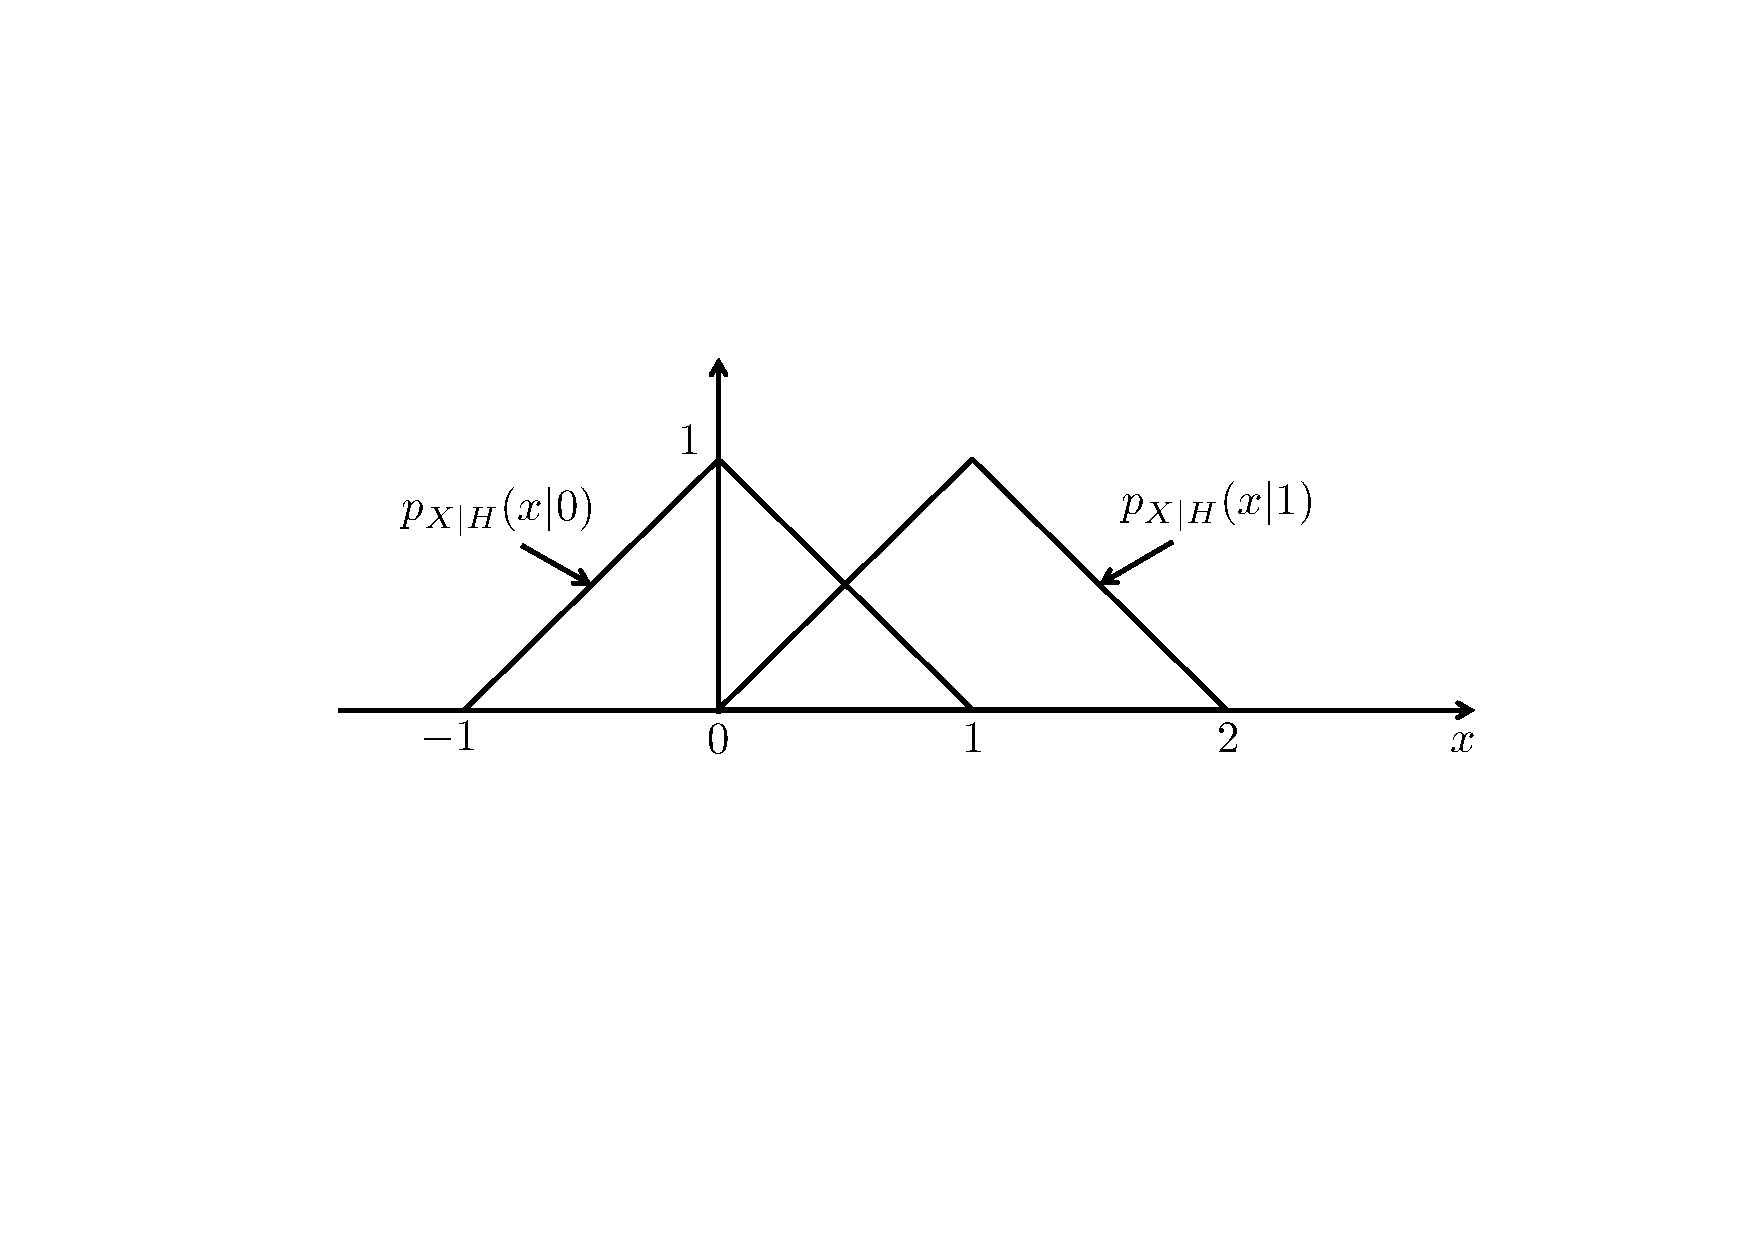
\includegraphics[scale=0.45]{Figuras/Fig_prob_dec.pdf}
\end{center}
\begin{parts}
\part Obtenga una expresión para las regiones de decisión de un decisor LRT genérico.
\part Obtenga las probabilidades de falsa alarma y de pérdida y represente la curva ROC.
\end{parts}

\else

We have a binary decision problem characterized by the likelihoods depicted in the following figure:
\begin{center}
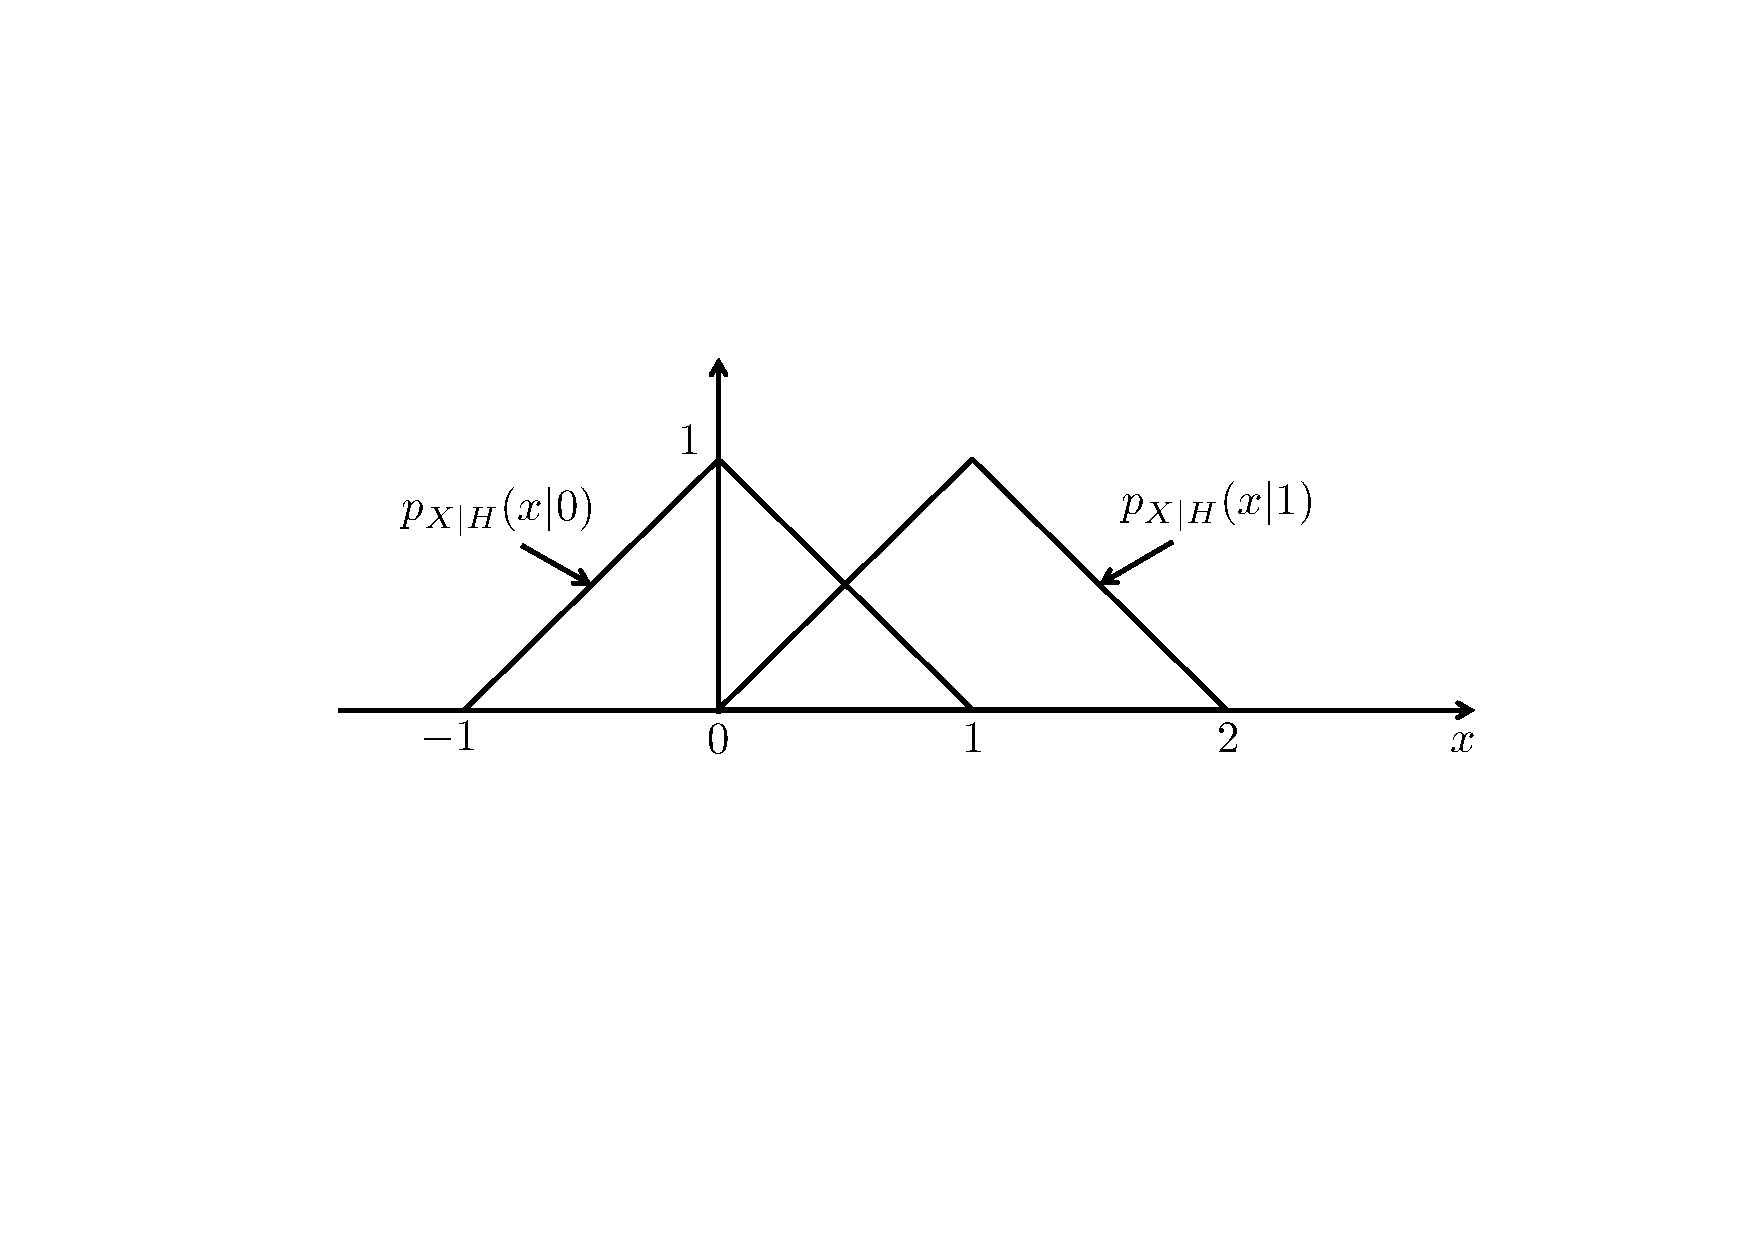
\includegraphics[scale=0.45]{Figuras/Fig_prob_dec.pdf}
\end{center}
\begin{parts}
\part Find an analytical expression for the decision regions of a generic LRT.
\part Obtain the probabilities of false alarm and missing, and plot the ROC curve.
\end{parts}

\fi 


\begin{solution}
\begin{parts}
\part $ \left \{
\begin{array}{ll}
-1 \le x \le 0  & D=0    \\
0 \le x \le 1   & x \dunodcero \dfrac{\eta}{1+\eta}=\nu \\
1 \le x \le 2   & D=1    \\
\end{array}
\right.$

\part 
$ \left \{
\begin{array}{ll}
-1 \le \nu \le 0  & \pmis=0 \\
0 < \nu < 1       & \pfa=\frac12 \left(1-\nu \right) ^2, \quad \pmis=\frac12 \nu^2 \\
1 \le \nu \le 2   & \pfa=0 \\
\end{array}
\right.$

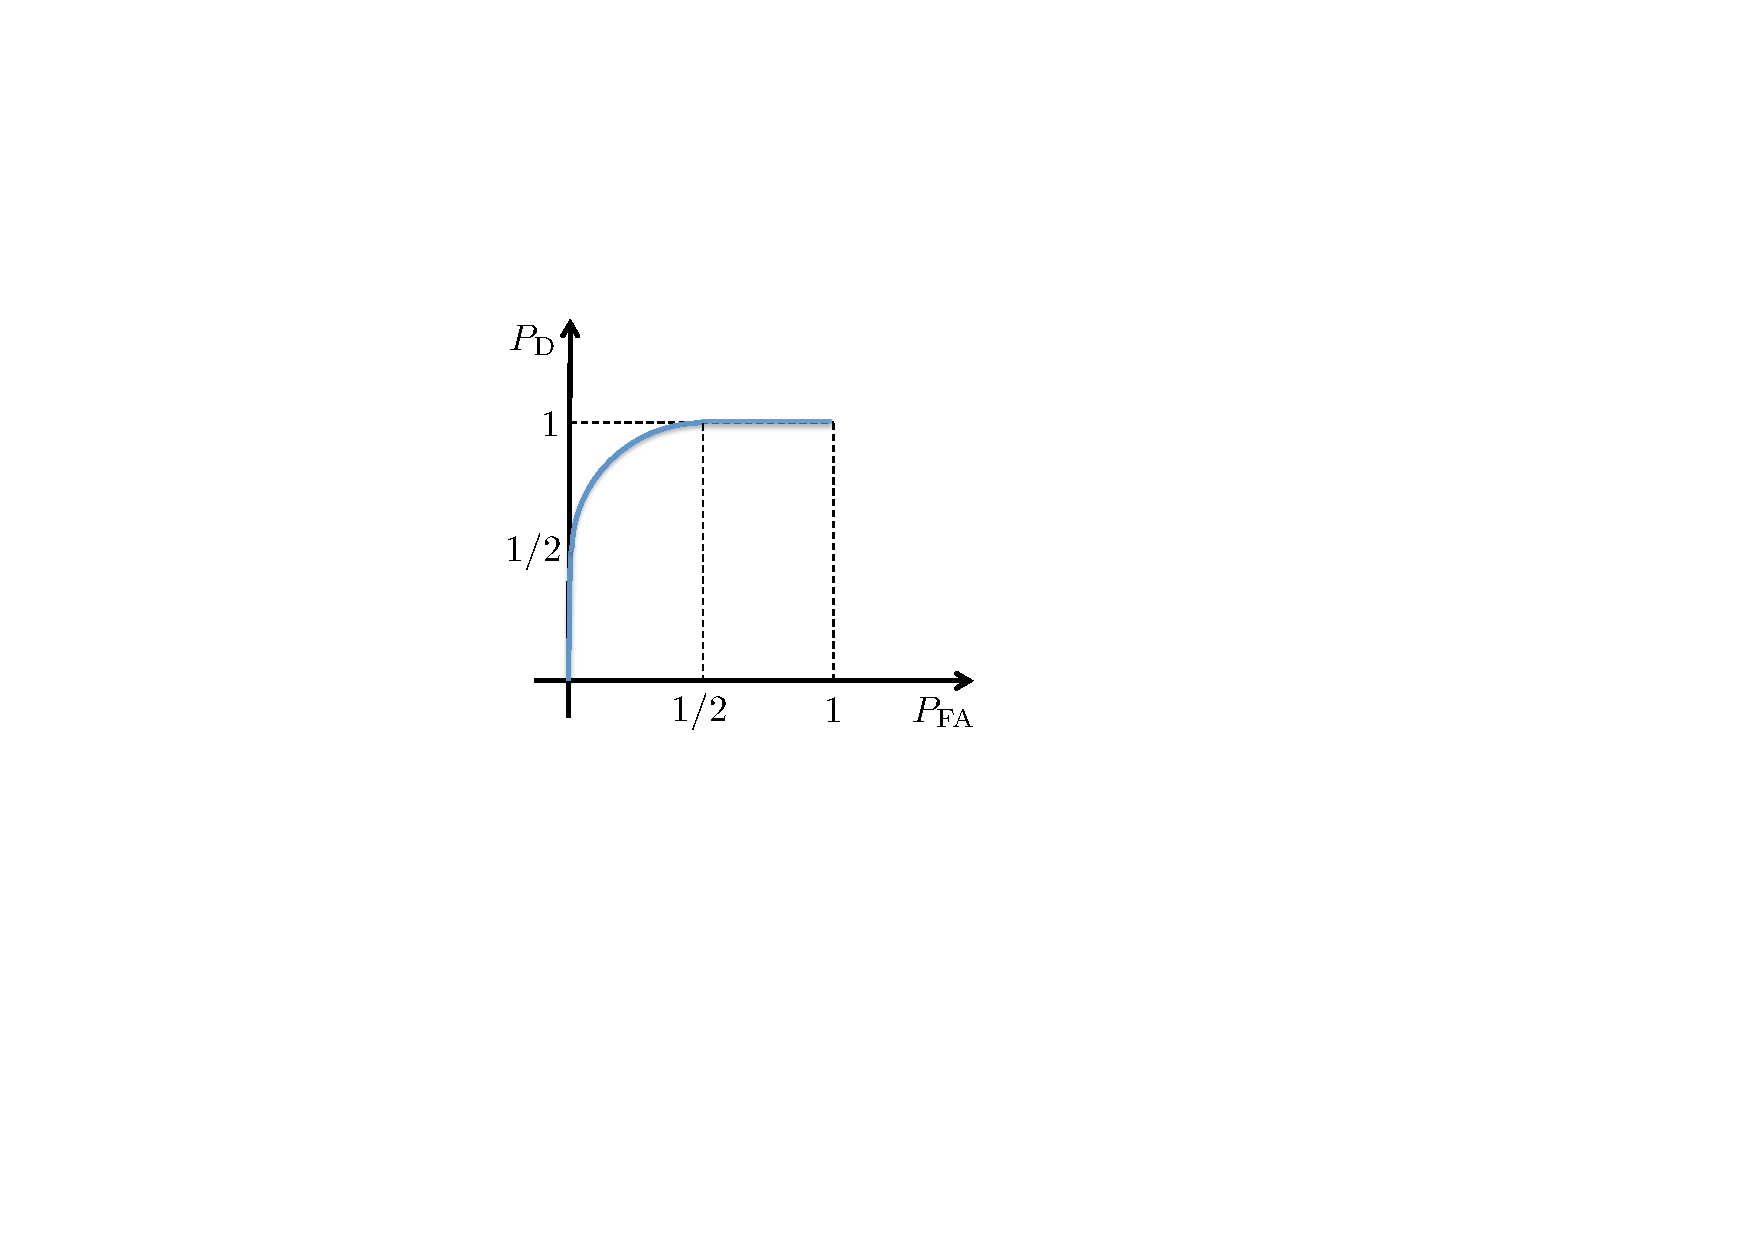
\includegraphics[scale=0.5]{Figuras/ROC_JUN2012}

This concludes.

\end{parts}

\end{solution}


%
%%%%%%%%%%%%%%%%%%%%%%%%%%%%%%%%%%%%%%%%%%%%%%%%%%%%%%%%%%%%%%%%%%%%
%%%%%%%%%%%%%% Junio 2012: Decision
\qformat{\textbf{\ej \thequestion ~~ (2.2; 2.5)} ~~ \linefill}
\ifspanish

\question Considere el problema de decisión binaria dado por hipótesis equiprobables y verosimilitudes
\begin{equation}
p_{x|H}(x|1) = x \exp(-x), \qquad x \ge 0
\end{equation}
\begin{equation}
p_{x|H}(x|0) = \exp(-x), \qquad x \ge 0
\end{equation}

\begin{parts}
\part Determine, en función de $\eta$, las regiones de decisión del decisor LRT de parámetro $\eta$.
\part Determine, en función de $\eta$, las probabilidades de falsa alarma y de pérdida del decisor LRT.
\part Determine la probabilidad de detección del detector de Neyman Pearson dado por $\pfa\le e^{-1}$.
\part Determine la probabilidad de error condicionada a la observación, $P\{D\neq H|x\}$, del decisor LRT de parámetro $\eta$
\end{parts}

%Indicación: $\int_0^\infty x^n \exp(-x) dx = n!$

\begin{solution}
\begin{parts}
\part $x\dunodcero \eta$
\part $\pfa = e^{-\eta}$, $\pfa = 1-(1+\eta)e^{-\eta}$ 
\part $\pdet = 2 e^{-1}$
\part $P\{D\neq H|x\} = \left[ \begin{array}{ll}
\frac{x}{1+x}, & \text{si } x<\eta  \\
\frac{1}{1+x}, & \text{si } x>\eta
\end{array}
\right.$
\end{parts}
\end{solution}

\else

\question Consider a binary decision problem with equally probable hypotheses and likelihoods
\begin{equation}
p_{x|H}(x|1) = x \exp(-x), \qquad x \ge 0
\end{equation}
\begin{equation}
p_{x|H}(x|0) = \exp(-x), \qquad x \ge 0
\end{equation}

\begin{parts}
\part Determine, as a function of $\eta$, the decision regions of an LRT decider with parameter $\eta$.
\part Obtain, as a function of $\eta$, the false alarm and missing probabilities of an LRT decider.
\part Calculate the probability of detection of a Neyman-Pearson classifier with $\pfa\le e^{-1}$.
\part Obtain the probability of error conditioned on the observation, $P\{D\neq H|x\}$, for an LRT decider with parameter $\eta$.
\end{parts}

%Indicación: $\int_0^\infty x^n \exp(-x) dx = n!$

\begin{solution}
\begin{parts}
\part $x\dunodcero \eta$
\part $\pfa = e^{-\eta}$, $\pfa = 1-(1+\eta)e^{-\eta}$ 
\part $\pdet = 2 e^{-1}$
\part $P\{D\neq H|x\} = \left[ \begin{array}{ll}
\frac{x}{1+x}, & \text{if } x<\eta  \\
\frac{1}{1+x}, & \text{if } x>\eta
\end{array}
\right.$
\end{parts}
\end{solution}

\fi
%
%%%%%%%%%%%%%%%%%%%%%%%%%%%%%%%%%%%%%%%%%%%%%%%%%%%%%%%%%%%%%%%%%%%%
%%%%%%%%%%%%%% Enero 2013: Decision MAP
\qformat{\textbf{\ej \thequestion ~~ (Decisión MAP binaria)} ~~ \linefill}
\question[20] % JCS 


\ifspanish

Considere el problema de decisión binaria dado por la observación $X\in[0,2]$ y verosimilitudes
\[
p_{X|H}(x|1) = \frac{1}{2} x
\]
\[
p_{X|H}(x|0) = \frac{3}{4}x(2-x)^2,
\]
siendo $P_H(1)= \dfrac{2}{5}$. 

\begin{parts}
\part Determine el decisor MAP.
\part Determine la probabilidad de pérdida del decisor MAP.
\part Suponga ahora que el mismo decisor que se ha obtenido en el apartado (a) se aplica a un escenario en el que la verosimilitud de $H=1$ es
\[
p'_{X|H}(x|1) = \frac{7}{8} p_{X|H}(x|1)
              + \frac{1}{16},
\]
mientras que la verosimilitud de $H=0$ sigue siendo la misma. Determine el incremento en la probabilidad de error que se produce como consecuencia de este cambio de escenario.
\end{parts}

\begin{solution}
\begin{parts}
\part $x \dunodcero \dfrac{4}{3}$
\part $\pmis = \dfrac{4}{9}$
\part Dado que la $\pfa$ no cambia y $\pmis' = \dfrac{17}{36}$, el incremento de la probabilidad de error es $P_H(1)(\pmis'-\pmis)=\dfrac{1}{90}$
\end{parts}
\end{solution}

\else

Consider the binary decision problem characterized by an observation $X\in[0,2]$ and likelihoods
\[
p_{X|H}(x|1) = \frac{1}{2} x
\]
\[
p_{X|H}(x|0) = \frac{3}{4}x(2-x)^2,
\]
with $P_H(1)= \dfrac{2}{5}$. 

\begin{parts}
\part Find the MAP classifier.
\part Obtain the probability of missing of the MAP classifier.
\part Assume now that the same decision maker that was designed in subsection (a) is applied to a scenario in which the likelihood of $H=1$ is
\[
p'_{X|H}(x|1) = \frac{7}{8} p_{X|H}(x|1)
              + \frac{1}{16},
\]
whereas the likelihood of $H=0$ remains unchanged. Obtain the increment in the probability of error that takes place as a consequence of this different scenario.
\end{parts}

\begin{solution}
\begin{parts}
\part $x \dunodcero \dfrac{4}{3}$
\part $\pmis = \dfrac{4}{9}$
\part Since $\pfa$ does not change and $\pmis' = \dfrac{17}{36}$, the increment of the probability of error is $P_H(1)(\pmis'-\pmis)=\dfrac{1}{90}$
\end{parts}
\end{solution}

\fi

%%%%%%%%%%%%%%%%%%%%%%%%%%%%%%%%%%%%%%%%%%%%%%%%%%%%%%%%%%%%%%%%%%%
%%%%%%%%%%%%% Enero 2013: Decision
\qformat{\textbf{\ej \thequestion ~~ (Decisión ML)} ~~ \linefill}
\ifspanish

\question[25] % MLG

Se toma una medida de la tensión intantánea $X$ existente en un momento dado en un nodo de un circuito. Bajo la hipótesis nula $H = 0$, en dicho nodo sólo existe ruido gaussiano de media nula y varianza $v$. Bajo la hipótesis $H=1$ en dicho nodo existe únicamente una señal sinusoidal de media nula y amplitud $\sqrt{v}$. Dado que se desconoce la frecuencia de la señal sinusoidal y el instante en el que se toma la medida, se tiene que bajo $H=1$ se mide $X =\sqrt{v} \cos \Phi$, con $\Phi$ una v.a. uniforme entre 0 y $2\pi$. 

\begin{parts}
\part Calcule las verosimilitudes de ambas hipótesis.
\part Calcule el decisor de máxima verosimilitud para discernir entre ellas.
\part Use la función $h(a) = a-\log(1-a)$ para expresar el decisor anterior y calcule las regiones de decisión en función de $v$ y $h^{-1}(\cdot)$.
\part Calcule la probabilidad de falsa alarma usando dicho decisor en función de $h^{-1}(\cdot)$ y $Q(z)$.
\end{parts}

Ayudas:

$$
\frac{d \cos u}{d u} = -\sin u  ~~~~ \frac{d \arccos u }{d u} = \frac{-1}{\sqrt{1-u^2}}~~~~\frac{d \sin u }{d u} = \cos u  ~~~~ \frac{d \arcsin u }{d u} = \frac{1}{\sqrt{1+u^2}}
$$

Suponga conocida la función $Q(z) = \int_{-\infty}^z \frac{1}{\sqrt{2\pi}} e^{-\frac{u^2}{2}} du $.

Suponga conocida la función $a = h^{-1}(\cdot)$ (función recíproca de $h(\cdot)$).


\begin{solution}
\begin{parts}
\part $p_{X|H}(x|0) = G(x|0,v)$, $p_{X|H}(x|1) = \frac{1}{\pi\sqrt{v-x^2}}~~\forall_{x\in[-\sqrt{v},\sqrt{v}]}$
\part $h(\frac{x^2}{v}) \dunodcero \log\frac{\pi}{2}$ si $x^2<v$, $D=0$ en otro caso.
\part $h^{-1}(\log\frac{\pi}{2}) = \frac{x^2}{v} = 0.2126 \approx 0.21 \Rightarrow$\\
$D_0: -\infty < x < -\sqrt{v} ~~\cup~~ -\sqrt{0.21v} < x < +\sqrt{0.21v}  ~~\cup~~ +\sqrt{v} < x < +\infty$\\
$D_1: -\sqrt{v} < x < -\sqrt{0.21v} ~~\cup~~  +\sqrt{0.21v} < x < +\sqrt{v} $
\part $\pfa = 2(Q(1)-Q(\sqrt{0.21}))$
\end{parts}
\end{solution}

\else

\question Let $X$ be a measurement of the instantaneous voltage at a circuit node. Under the null hypothesis $H = 0$, the voltage at the node is characterized by a Gaussian noise with mean 0 and variance $v$. Under hypothesis $H=1$, in such node there exists just a sinusoidal signal with mean zero and amplitude $\sqrt{v}$. Since the frequency of the signal is not known, we have that under $H=1$ the measurement can be probabilistically modeled as $X =\sqrt{v} \cos \Phi$, with $\Phi$ a random variable with uniform distribution between 0 and $2\pi$. 

\begin{parts}
\part Calculate the likelihoods of both hypotheses.
\part Find the maximum likelihood test to discriminate among them.
\part Use function $h(a) = a-\log(1-a)$ to express the ML classifier, and calculate the decision regions as functions of $v$ and $h^{-1}(\cdot)$.
\part Obtain the probability of false alarm of such decision maker as a function of $h^{-1}(\cdot)$ and $Q(z)$.
\end{parts}

Hints:

$$
\frac{d \cos u }{d u} = -\sin u  ~~~~ \frac{d \arccos u }{d u} = \frac{-1}{\sqrt{1-u^2}}~~~~\frac{d \sin u }{d u} = \cos u  ~~~~ \frac{d \arcsin u }{d u} = \frac{1}{\sqrt{1+u^2}}
$$

Assume as known function $Q(z) = \int_{-\infty}^z \frac{1}{\sqrt{2\pi}} e^{-\frac{u^2}{2}} du $.

Assume as known function $a = h^{-1}(\cdot)$ (reciprocal function of $h(\cdot)$).

\begin{solution}
\begin{parts}
\part $p_{X|H}(x|0) = G(x|0,v)$, $p_{X|H}(x|1) = \frac{1}{\pi\sqrt{v-x^2}}~~\forall_{x\in[-\sqrt{v},\sqrt{v}]}$
\part $h(\frac{x^2}{v}) \dunodcero \log\frac{\pi}{2}$ if $x^2<v$; $D=0$ otherwise.
\part $h^{-1}(\log\frac{\pi}{2}) = \frac{x^2}{v} = 0.2126 \approx 0.21 \Rightarrow$\\
$D_0: -\infty < x < -\sqrt{v} ~~\cup~~ -\sqrt{0.21v} < x < +\sqrt{0.21v}  ~~\cup~~ +\sqrt{v} < x < +\infty$\\
$D_1: -\sqrt{v} < x < -\sqrt{0.21v} ~~\cup~~  +\sqrt{0.21v} < x < +\sqrt{v} $
\part $P_\text{FA} = 2(Q(1)-Q(\sqrt{0.21}))$
\end{parts}
\end{solution}

\fi

%%%%%%%%%%%%%%%%%%%%%%%%%%%%%%%%%%%%%%%%%%%%%%%%%%%%%%%%%%%%%%%%%%%
%%%%%%%%%%%%% Cuestión III, Jul 2013)
\qformat{\textbf{\ej \thequestion ~~ (Decisión bayesiana)} ~~ \linefill}
\ifspanish

\question[20] % JCS 

Considere el problema de decisión binario dado por las verosimilitudes:
$$ \begin{array}{ll}
p_{X|H}(x|0) = \exp (-x), & \quad x>0 \\
p_{X|H}(x|1) = \sqrt{\frac{2}{\pi}} \exp (- \frac{x^2}{2}), & \quad x>0\\
\end{array} $$

Sabiendo que $P_H(0) = \displaystyle \sqrt{\frac{2}{\pi}} P_H(1)$ y $c_{00} = c_{11} = 0$, $c_{10} = \displaystyle \exp\left( \frac{1}{2}\right) c_{01}$:

\begin{parts}
\part Determine las regiones de decisión del decisor MAP.
\part Calcule la probabilidad de error del decisor MAP. Exprese su resultado utilizando la función:
$$F(x) = 1- Q(x) = \int_{-\infty}^x \frac{1}{\sqrt{2\pi}} \exp{\left( - \frac{t^2}{2}\right) } \; dt$$
\part Determine las regiones de decisión del decisor bayesiano de mínimo coste medio.
\part Calcule la probabilidad de error del decisor obtenido en el apartado anterior.
\end{parts}

\begin{solution}
\begin{parts}
\part $x \dceroduno 2$ \\ $P_e= \displaystyle \frac{1}{1+\sqrt{\frac{2}{\pi}}} \left[ \sqrt{\frac{2}{\pi}} \left( 1-\exp(-2)\right) + 2 -2F(2) \right] $
\part Siempre se decide $D=0$, $P_e= \displaystyle \frac{1}{\sqrt{\frac{2}{\pi}}+1}$
\end{parts}
\end{solution}

\else

\question Consider a binary decision problem characterized by the following likelihoods:
$$ \begin{array}{ll}
p_{X|H}(x|0) = \exp (-x), & \quad x>0 \\
p_{X|H}(x|1) = \sqrt{\frac{2}{\pi}} \exp (- \frac{x^2}{2}), & \quad x>0\\
\end{array} $$

It is also known that $P_H(0) = \displaystyle \sqrt{\frac{2}{\pi}} P_H(1)$ and $c_{00} = c_{11} = 0$, $c_{10} = \displaystyle \exp\left( \frac{1}{2}\right) c_{01}$:

\begin{parts}
\part Find the decision regions of the MAP classifier.

\part Calculate the probability of error of the MAP classifier. Express your result by means of function:
$$F(x) = 1- Q(x) = \int_{-\infty}^x \frac{1}{\sqrt{2\pi}} \exp{\left( - \frac{t^2}{2}\right) } \; dt$$

\part Determine the decision regions of the Bayesian classifier with minimum risk.

\part Calculate the probability of error of the decision maker obtained in the previous subsection.

\end{parts}

\begin{solution}
\begin{parts}
\part $x \dceroduno 2$ \\ $P_e= \displaystyle \frac{1}{1+\sqrt{\frac{2}{\pi}}} \left[ \sqrt{\frac{2}{\pi}} \left( 1-\exp(-2)\right) + 2 -2F(2) \right] $
\part This classifier always decides $D=0$, $P_e= \displaystyle \frac{1}{\sqrt{\frac{2}{\pi}}+1}$
\end{parts}
\end{solution}

\fi

%%%%%%%%%%%%%%%%%%%%%%%%%%%%%%%%%%%%%%%%%%%%%%%%%%%%%%%%%%%%%%%%%%%
%%%%%%%%%%%%% Cuestión V: Decisión No-bayesiana
\qformat{\textbf{\ej \thequestion ~~ (Decisión no bayesiana)} ~~ \linefill}
\ifspanish

\question[25] % 

Considere el problema de decisión dado por las verosimilitudes:
\begin{align}
p_{X|H}(x|1) &= \frac{\pi}{2} \sin\left(\frac{\pi}{2}x\right), \qquad 0<x<1 \nonumber\\
p_{X|H}(x|0) &= \frac{\pi}{2} \cos\left(\frac{\pi}{2}x\right), \qquad 0<x<1\nonumber
\end{align}

\begin{parts}
\part Determine las regiones de decisión del decisor LRT de parámetro $\eta$:
$$\frac{p_{X|H}(x|1)}{p_{X|H}(x|0)}\dunodcero \eta.$$
\part Represente gráficamente, de forma aproximada, la ROC del decisor LRT.
\part Represente, sobre la ROC, el punto de operación del decisor ML.
\part Represente, sobre la ROC, el punto de operación del decisor minimax.
\part Represente, sobre la ROC, el punto de operación del decisor de Neyman Pearson con $\pfa \le 0.4$.
\end{parts}

\begin{solution}
\begin{parts}
\part $x \dunodcero \dfrac{2}{\pi} \arctan(\eta)$, 
\part La ROC es un arco de circunferencia de radio 1 y centrado en (1,0).
\part $(\pfa,\pdet)= \left(1-\dfrac{\sqrt 2}{2},\dfrac{\sqrt 2}{2}\right)$
\part $(\pfa,\pdet)= \left(1-\dfrac{\sqrt 2}{2},\dfrac{\sqrt 2}{2}\right)$
\part $(\pfa,\pdet)= \left(0.4,0.8\right)$
\end{parts}
\end{solution}

\else

\question Consider a binary decision problem with likelihoods:
\begin{align}
p_{X|H}(x|1) &= \frac{\pi}{2} \sin\left(\frac{\pi}{2}x\right), \qquad 0<x<1 \nonumber\\
p_{X|H}(x|0) &= \frac{\pi}{2} \cos\left(\frac{\pi}{2}x\right), \qquad 0<x<1\nonumber
\end{align}

\begin{parts}
\part Find the decision regions of an LRT decision maker with parameter $\eta$:
$$\frac{p_{X|H}(x|1)}{p_{X|H}(x|0)}\dunodcero \eta.$$
\part Provide an approximate plot of the ROC of the LRT classifier.
\part Indicate which point of the ROC corresponds to the operating point of the ML classifier.
\part Indicate which point of the ROC corresponds to the operating point of the minimax decision maker.
\part Indicate which point of the ROC corresponds to the operating point of Neyman Pearson detector with $\pfa \le 0.4$.
\end{parts}

\begin{solution}
\begin{parts}
\part $x \dunodcero \dfrac{2}{\pi} \arctan(\eta)$, 
\part The ROC is a circumference arch of radius 1, and centered in (1,0).
\part $(\pfa,\pmis)= \left(1-\dfrac{\sqrt 2}{2},\dfrac{\sqrt 2}{2}\right)$
\part $(\pfa,\pmis)= \left(1-\dfrac{\sqrt 2}{2},\dfrac{\sqrt 2}{2}\right)$
\part $(\pfa,\pmis)= \left(0.4,0.8\right)$
\end{parts}
\end{solution}

\fi

%%%%%%%%%%%%%%%%%%%%%%%%%%%%%%%%%%%%%%%%%%%%%%%%%%%%%%%%%%%%%%%%%%%
%%%%%%%%%%%%% Enero 2014, Cuestión III: Decision
\qformat{\textbf{\ej \thequestion ~~ (Decisión bayesiana y Neyman-Pearson)} ~~ \linefill}
\ifspanish

\question[20] % JCS 

Considere el problema de decisión binaria dado por la observación $X\in[0,4]$ y verosimilitudes
\[
p_{X|H}(x|0) = \frac{1}{8} x,  \qquad 0\le x \le 4
\]
\[
p_{X|H}(x|1) = c x\exp(-x),  \qquad 0\le x \le 4,
\] 
siendo $c=\left(1-5\exp(-4)\right)^{-1}$.
%siendo $c=\left(1-(a+1)\exp(-a)\right)^{-1}$.

\begin{parts}
\part Determine las regiones de decisión de un decisor LRT de parámetro $\eta$.
\part Determine para qué valores de $\eta$ se verifica $P\{D=0\}=1$.
\part Determine el decisor de Neyman-Pearson con $\pfa\le 0.1$.
\end{parts}

\begin{solution}
\begin{parts}
\part $x \dceroduno \ln\left(\frac{8c}{\eta}\right)$
\part $\eta \ge 8 c$
\part $x \dceroduno \sqrt{1.6}$
\end{parts}
\end{solution}

\else

\question[20] % JCS 

Consider the binary decision problem given by observation $X\in[0,4]$ and likelihoods
\[
p_{X|H}(x|0) = \frac{1}{8} x,  \qquad 0\le x \le 4
\]
\[
p_{X|H}(x|1) = c x\exp(-x),  \qquad 0\le x \le 4,
\] 
where $c=\left(1-5\exp(-4)\right)^{-1}$.
%siendo $c=\left(1-(a+1)\exp(-a)\right)^{-1}$.

\begin{parts}
\part Find the decision regions of the LRT decision maker with parameter $\eta$.
\part Find the values of $\eta$ for which $P\{D=0\}=1$.
\part Find the Neyman-Pearson detector with $\pfa\le 0.1$.
\end{parts}

\begin{solution}
\begin{parts}
\part $x \dceroduno \ln\left(\frac{8c}{\eta}\right)$
\part $\eta \ge 8 c$
\part $x \dceroduno \sqrt{1.6}$
\end{parts}
\end{solution}

\fi

%%%%%%%%%%%%%%%%%%%%%%%%%%%%%%%%%%%%%%%%%%%%%%%%%%%%%%%%%%%%%%%%%%%
%%%%%%%%%%%%% Enero 2014, Cuestión V: Decision
\qformat{\textbf{\ej \thequestion ~~ (Decisión gaussiana)} ~~ \linefill}
\ifspanish

\question[30] % MLG

Las variables aleatorias $Z_1$ y $Z_2$ sólo pueden tomar los valores $-m$ o $m$. Bajo hipótesis $H=0$, ambas variables toman el mismo valor. Esto conduce a dos posibles configuraciones bajo esta hipótesis, ambas con la misma probabilidad. Bajo hipótesis $H=1$, ambas variables toman diferentes valores. Esto conduce a dos posibles configuraciones bajo esta hipótesis, ambas con al misma probabilidad. Las hipótesis $H=0$ y $H=1$ son equiprobables.

Las variables $Z_1$ y $Z_2$ no pueden observarse directamente. Sin embargo, podemos observar $X_1$ y $X_2$, que son medidas ruidosas de $Z_1$ and $Z_2$ respectivamente, mediante un dispositivo que añade ruido gausiano de media nula y varianza unidad, es decir, $X_i=Z_i+N_i$, siendo $N_1$ y $N_2$ independientes entre sí e independientes de $Z_1$ y $Z_2$.

\begin{parts}
\part Determine $P_{Z_1,Z_2|H}(z_1,z_2|h)$ para todos los posibles valores de $z_1$, $z_2$ y $h$.
\part Determine $P_{X_1,X_2|Z_1,Z_2}(x_1,x_2|z_1,z_2)$. 
\part Sin hacer cálculos, razone si $$P_{X_1,X_2|Z_1,Z_2}(x_1,x_2|z_1,z_2)$$ es diferente o idéntica a $P_{X_1,X_2|Z_1,Z_2,H}(x_1,x_2|z_1,z_2,h)$. 
\part Determine las verosimilitudes de las hipótesis, $P_{X_1,X_2|H}(x_1,x_2|0)$ y $p_{X_1,X_2|H}(x_1,x_2|1)$. 
\part Determine el decisor MAP para las observaciones $x_1$ y $x_2$.\\
\end{parts}

\begin{solution}
\begin{parts}
\part $P_{Z_1,Z_2|H}(m,m|0)=P_{Z_1,Z_2|H}(-m,-m|0)=\frac12$

$P_{Z_1,Z_2|H}(m,-m|1)=P_{Z_1,Z_2|H}(-m,m|1)=\frac12$,

$P_{Z_1,Z_2|H}(-m,m|0)=P_{Z_1,Z_2|H}(m,-m|0)=0$,

$P_{Z_1,Z_2|H}(-m,-m|1)=P_{Z_1,Z_2|H}(m,m|1)=0$
\part $\begin{bmatrix} x_1 \\ x_2 \end{bmatrix} \sim \mathcal{N}\left(\begin{bmatrix} z_1 \\ z_2 \end{bmatrix}, \begin{bmatrix} 1 & 0 \\0 & 1 \end{bmatrix}\right)$
\part Es idéntica, ya que $x_1$ y $x_2$ son independientes de $h$ condicionalmente en $z_1$ y $z_2$.
\part $P_{X_1,X_2|H}(x_1,x_2|0) = \frac12 \mathcal{N}\left(\begin{bmatrix} m \\ m \end{bmatrix}, \begin{bmatrix} 1 & 0 \\0 & 1 \end{bmatrix}\right) + \frac12 \mathcal{N}\left(\begin{bmatrix} -m \\ -m \end{bmatrix}, \begin{bmatrix} 1 & 0 \\0 & 1 \end{bmatrix}\right)$

$P_{X_1,X_2|H}(x_1,x_2|1) = \frac12 \mathcal{N}\left(\begin{bmatrix} -m \\ m \end{bmatrix}, \begin{bmatrix} 1 & 0 \\0 & 1 \end{bmatrix}\right) + \frac12 \mathcal{N}\left(\begin{bmatrix} m \\ -m \end{bmatrix}, \begin{bmatrix} 1 & 0 \\0 & 1 \end{bmatrix}\right)$
\part Decide 0 para $x_1x_2>0$, 1 en otro caso.

\end{parts}
\end{solution}

\else

\question[30] % MLG

Variables $Z_1$ and $Z_2$ can only take values, $-m$ or $m$. Under hypothesis $H=0$, both variables take the same value. This yields two possible configurations under this hypothesis, both appearing with the same probability. Under hypothesis $H=1$, both variables take different values. This yields two possible configurations under this hypothesis, both appearing with the same probability. Hypotheses $H=0$ and $H=1$ are equiprobable.

Variables $z_1$ and $Z_2$ cannot be observed directly. However, we can observe $X_1$ and $X_2$, which are noisy measurements of $Z_1$ and $Z_2$ respectively, using a device that adds independent zero-mean Gaussian noise of variance one, i. e., $X_i=Z_i+N_i$, where $N_1$ and $N_2$ are independent and also independent of $Z_1$ and $Z_2$.


\begin{parts}
\part Compute $P_{Z_1,Z_2|H}(z_1,z_2|h)$ for all possible values of $z_1$, $z_2$ and $i$.
\part Compute $P_{X_1,X_2|Z_1,Z_2}(x_1,x_2|z_1,z_2)$. 
\part Without making any computations, reason whether $$P_{X_1,X_2|Z_1,Z_2}(x_1,x_2|z_1,z_2)$$ is different or identical to $P_{X_1,X_2|Z_1,Z_2,H}(x_1,x_2|z_1,z_2,h)$.
\part Compute the likelihoods of both hypotheses, $P_{X_1,X_2|H}(x_1,x_2|0)$ and $p_{X_1,X_2|H}(x_1,x_2|1)$. 
\part Compute the MAP decider given observations $x_1$ and $x_2$.\\
\end{parts}

\begin{solution}
\begin{parts}
\part 
\end{parts}
\end{solution}

\fi

%%%%%%%%%%%%%%%%%%%%%%%%%%%%%%%%%%%%%%%%%%%%%%%%%%%%%%%%%%%%%%%%%%%
%%%%%%%%%%%%% Junio 2014, Cuestión III: Decision
\qformat{\textbf{\ej \thequestion ~~ (Decisión bayesiana, ROC, min-max)} ~~ \linefill}
\ifspanish

\question[20] % JCS 

Considere el problema de decisión binaria dado por la observación $X\in\left[0,\dfrac{\pi}{2}\right]$ y verosimilitudes
\[
p_{X|H}(x|0) = \cos(x),  \qquad 0\le x \le \frac{\pi}{2}
\]
\[
p_{X|H}(x|1) = \sen(x),  \qquad 0\le x \le \frac{\pi}{2},
\] 

\begin{parts}
\part Determine las regiones de decisión de un decisor LRT de parámetro $\eta \ge 0$.
\part Determine la ROC. 
\part Determine las regiones de decisión del decisor minimax.
\end{parts}

Indicación: para todo $\alpha \in \mathbb{R}$, $\cos(\arctan(\alpha)) = \dfrac{1}{\sqrt{\alpha^2+1}}$

\begin{solution}
\begin{parts}
\part $x \dunodcero \arctan(\eta)$
\part $\pdet = \sqrt{\pfa(1-\pfa)}$
\part $x \dunodcero \dfrac{\pi}{4}$
\end{parts}
\end{solution}

\else

\question[20] % JCS 

Consider the binary decision problem given by observation $X\in\left[0,\dfrac{\pi}{2}\right]$ and likelihoods
\[
p_{X|H}(x|0) = \cos(x),  \qquad 0\le x \le \frac{\pi}{2}
\]
\[
p_{X|H}(x|1) = \sin(x),  \qquad 0\le x \le \frac{\pi}{2},
\] 

\begin{parts}
\part Compute the decision regions of an LRT decision maker with parameter $\eta \ge 0$.
\part Compute the ROC. 
\part Compute the decision regions of a minimax decision maker.
\end{parts}

Hint: for any $\alpha\in \mathbb{R}$, $\cos(\arctan(\alpha)) = \dfrac{1}{\sqrt{\alpha^2+1}}$

\begin{solution}
\begin{parts}
\part $x \dunodcero \arctan(\eta)$
\part $\pdet = \sqrt{\pfa(1-\pfa)}$
\part $x \dunodcero \dfrac{\pi}{4}$
\end{parts}
\end{solution}

\fi

%%%%%%%%%%%%%%%%%%%%%%%%%%%%%%%%%%%%%%%%%%%%%%%%%%%%%%%%%%%%%%%%%%%
%%%%%%%%%%%%% Junio 2014, Cuestión V: Decision
\qformat{\textbf{\ej \thequestion ~~ (Decisión bayesiana)} ~~ \linefill}
\ifspanish

\question[25] % JCS

Considere el problema de decisión dado por hipótesis equiprobables y observaciones $X_1,X_2,X_3$, independientes entre sí bajo cualquiera de las hipótesis, e idénticamente distribuidas, con verosimilitudes
\begin{align}
p_{X_n|H}(x|1) &= \exp(- x) u(x)       , \qquad  \qquad n=1,2,3 \nonumber\\
p_{X_n|H}(x|0) &= 2 \exp(- 2 x) u(x)   \qquad  \qquad n=1,2,3 \nonumber 
\end{align}
Se aplican tres decisores MAP, uno por cada variable, de tal modo que la decisión $D_n$ del decisor $n$-ésimo está basada solamente en la observación $X_n$ (para $n=1$, 2 o 3).

\begin{parts}
\part Determine las probabilidades de falsa alarma, pérdida y error de cada decisor.
\part Determine la probabilidad de que, bajo hipótesis $H=0$, los tres decisores tomen la misma decisión. 
\part Sea ${\bf Z} = (D_1,D_2,D_3)$ el vector que contiene las tres decisiones. Considere el decisor MAP basado en la observación de ${\bf Z}$ (es decir, el decisor no observa $X_1$, $X_2$ o $X_3$, y su entrada es ${\bf Z}$). Determine su decisión cuando ${\bf Z} = (1,1,0)$.
\end{parts}

\begin{solution}
\begin{parts}
\part $\pmis  = \dfrac{1}{2}$, $\pfa = \dfrac{1}{4}$, $P_e = \dfrac{3}{8}$.
\part $P = \dfrac{7}{64}$.
\part Decide $1$.
\end{parts}
\end{solution}

\else

\question[25] % JCS

Consider the decision problem given by equally likely hypothesis and observations $X_1,X_2,X_3$ that are independent under any of the hypothesis, and identically distributed, with likelihoods
\begin{align}
p_{X_n|H}(x|1) &= \exp(- x) u(x)       , \qquad  \qquad n=1,2,3 \nonumber\\
p_{X_n|H}(x|0) &= 2 \exp(- 2 x) u(x)   \qquad  \qquad n=1,2,3 \nonumber 
\end{align}
Three MAP classifiers are applied, one for each variable, in such a way that decision $D_n$ of the $n$-th decision maker is based in observation $X_n$ only (for $n=1$, 2 or 3). 

\begin{parts}
\part Determine the false alarm, missing and error probability of each decision maker.
\part Determine the probability that all decision makers take the same decision, given $H=0$. 
\part Let $Z = (D_1,D_2,D_3)$ the vector containing the three decisions. Consider the MAP classifier based on observation ${\bf Z}$ (that is, the decision maker does not observe $X_1$, $X_2$ or $X_3$, and its only input is ${\bf Z}$). Determine its decision when ${\bf Z} = (1,1,0)$.
\end{parts}

\begin{solution}
\begin{parts}
\part $\pmis  = \dfrac{1}{2}$, $\pfa = \dfrac{1}{4}$, $P_e = \dfrac{3}{8}$.
\part $P = \dfrac{7}{64}$.
\part $D_1+D_2+D_3 \dunodcero \dfrac{3}{2}$.
\end{parts}
\end{solution}

\fi

%%%%%%%%%%%%%%%%%%%%%%%%%%%%%%%%%%%%%%%%%%%%%%%%%%%%%%%%%%%%%%%%%%%
%%%%%%%%%%%%% Enero 2015, Q3
\qformat{\textbf{\ej \thequestion ~~ (Decisión MAP)} ~~ \linefill}
\ifspanish

\question[20] % VGV

Se dispone de un sistema de comunicaciones en el que el transmisor envía, con la misma probablidad a priori, un único símbolo (``$+1$'' ó ``$-1$'') de manera simultánea por dos canales ruidosos, tal y como se ilustra en la figura:
\begin{center}
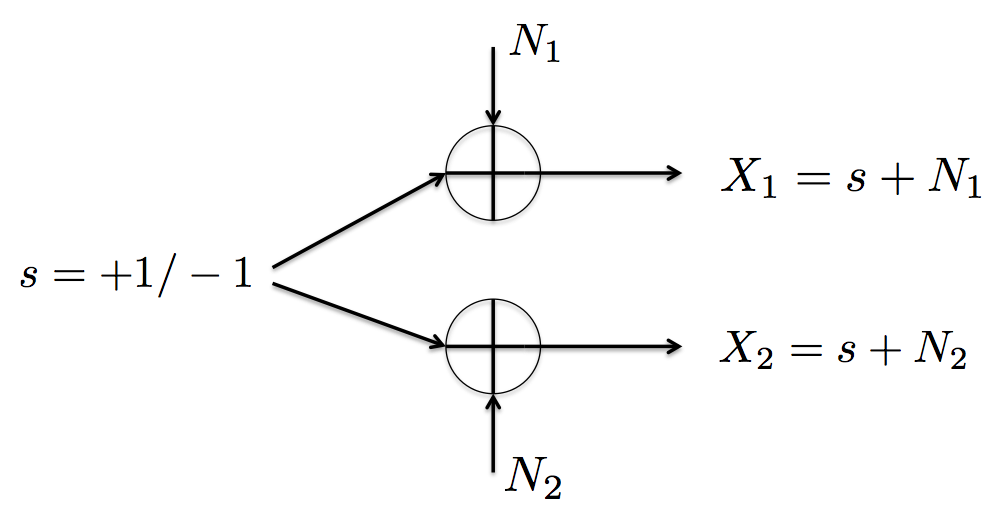
\includegraphics[width=8cm]{Figuras/Fig_canal_gauss}
\end{center}

donde $N_1$ y $N_2$ son dos variables de ruido gaussiano, independientes entre si, con medias nulas y varianzas $\lambda v$ y $(1- \lambda) v$, respectivamente, y $v>0$ y $0 \leq \lambda \leq 1$ son constantes conocidas.
\begin{parts}
\part Obtenga el decisor de mínima probabilidad de error, basado en la observación conjunta de $X_1$ y $X_2$, que permite al receptor saber si se transmitió el símbolo ``$+1$'' ó ``$-1$''.
\part Obtenga la probabilidad de error del decisor anterior.  Exprese su resultado utilizando la función:
$$F(x) = 1- Q(x) = \int_{-\infty}^x \frac{1}{\sqrt{2\pi}} \exp{\left( - \frac{t^2}{2}\right) } \; dt$$

\part Analice el comportamiento del decisor (frontera de decisión y probabilidad de error) para los casos: $\lambda=0$ y $\lambda=1$.
\end{parts}

\begin{solution}

\begin{parts}
\part $(1-\lambda)x_1 + \lambda x_2 \dunodcero 0$
\part $\displaystyle  P_{\rm e}=F(-\frac{1}{\sqrt{\lambda(1-\lambda)v}})$ 
\part Si $\lambda=0$, $X_2=s$ (tiene varianza nula) y solo se usa esta observación para decidir. $P_{\rm e}=0$. Si $\lambda=1$ ocurre lo mismo pero con $X_1$.
\end{parts}
 \end{solution}

\else

\question[20] % VGV

Consider a communication system where the transmitter sends, with equal {\em a priori} probabilities, the same symbol ``$+1$'' or ``$-1$'' through two noisy channels, as illustrated in the figure:
\begin{center}
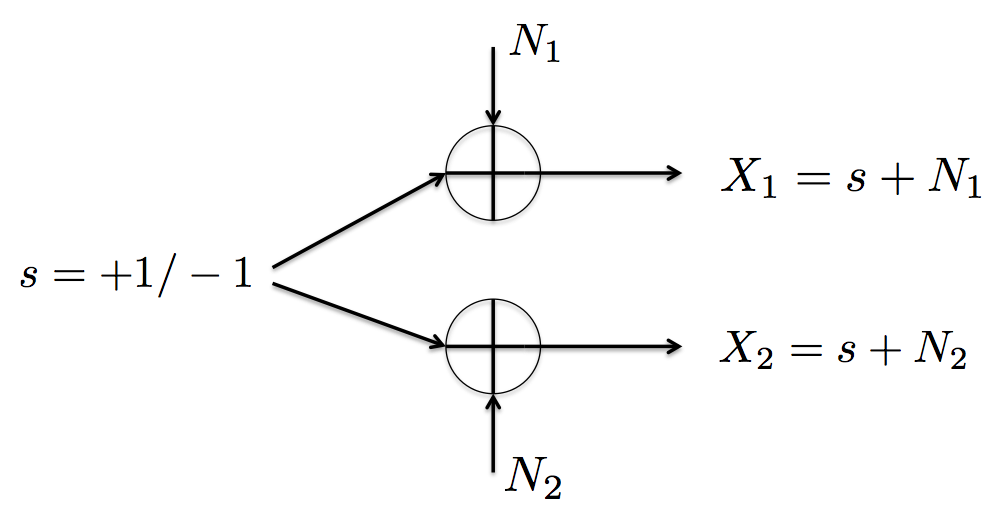
\includegraphics[width=8cm]{Figuras/Fig_canal_gauss}
\end{center}
where $N_1$ and $N_2$ are independent Gaussian random variables, with zero mean and variances $\lambda v$ and $(1-\lambda) v$, respectively; $v>0$ and $0 \leq \lambda \leq 1$ are two known constants.

\begin{parts}
\part Obtain the binary classifier with a minimum probability of error, based on the joint observation of $X_1$ and $X_2$, which allows the receiver to decide whether the transmitted symbol was $+1$ or $-1$.
\part Compute the error probability of the above decision maker. Express your result by means of the function
$$F(x) = 1- Q(x) = \int_{-\infty}^x \frac{1}{\sqrt{2\pi}} \exp{\left( - \frac{t^2}{2}\right) } \; dt$$
\part Analyze the behaviour of the decision maker (i.e., its decision rule and probability of error) when: $\lambda=0$ and $\lambda=1$.
\end{parts}

\begin{solution}
\begin{parts}
\part $(1-\lambda)x_1 + \lambda x_2 \dunodcero 0$
\part $\displaystyle  P_{\rm e}=F(-\frac{1}{\sqrt{\lambda(1-\lambda)v}})$ 
\part When $\lambda=0$, $X_2=s$ (its variance is zero) and we only consider this observation to make the decision. $P_{\rm e}=0$. When  $\lambda=1$ a similar behaviour happens, but considering observation $X_1$.
\end{parts}
\end{solution}

\fi

%%%%%%%%%%%%%%%%%%%%%%%%%%%%%%%%%%%%%%%%%%%%%%%%%%%%%%%%%%%%%%%%%%%
%%%%%%%%%%%%% Enero 2015, Q5
\qformat{\textbf{\ej \thequestion ~~ (LRT, ROC, Minimax, NP)} ~~ \linefill}
\ifspanish

\question[25] % JCS

Considere el problema de decisión binario dado por hipótesis equiprobables y verosimilitudes
$$p_{X|H}(x|1) = \frac{1}{(1+x)^2}, \qquad x\ge 0$$
$$p_{X|H}(x|0) = \frac{2x}{(1+x)^3}, \qquad x\ge 0$$
\begin{parts}
\part Determine las regiones de decisión del decisor LRT de parámetro $\eta$.
\part Represente de forma aproximada la ROC del LRT.
\part Determine las regiones de decisión del decisor minimax.
\part Determine las regiones de decisión del decisor de Neyman-Pearson con $\pfa \le \dfrac{1}{16}$
%\part Determine el decisor LRT que verifica $P\{D=0\} = P\{D=1\}$.
\end{parts}
Indicación: las funciones de distribución para las verosimilitudes dadas son:
$$F_{X|H}(x|1) = \frac{x}{(1+x)}, \qquad x\ge 0$$
$$F_{X|H}(x|0) = \frac{x^2}{(1+x)^2}, \qquad x\ge 0$$

\begin{solution}
\begin{parts}
\part Si $\eta>\dfrac{1}{2}$, $x\dceroduno \dfrac{1}{2\eta-1}$. 

Si $\eta<\frac12$, el decisor LRT decide siempre $D=1$.
\part $\pdet = \sqrt{\pfa}$
\part $x\dceroduno \dfrac{1}{2}(1+\sqrt{5})$ 
\part $x\dceroduno \dfrac{1}{3}$ 
\part $x\dceroduno \dfrac{1}{2}(1+\sqrt{5})$ 
\end{parts}
\end{solution}

\else

\question[25] % JCS

Consider the binary decision problem given by equally probable hypothesis and likelihoods
$$p_{X|H}(x|1) = \frac{1}{(1+x)^2}, \qquad x\ge 0$$
$$p_{X|H}(x|0) = \frac{2x}{(1+x)^3}, \qquad x\ge 0$$
\begin{parts}
\part Compute the decision regions of the LRT decision maker with parameter $\eta$.
\part Sketch the ROC of LRT approximately.
\part Compute the decision regions of the minimax decision maker.
\part Compute the decision regions of the Neyman-Pearson decision maker with $\pfa \le \dfrac{1}{16}$
%\part Compute the LRT decision maker satisfying $P\{D=0\} = P\{D=1\}$.
\end{parts}
Hint: the probability distribution functions corresponding to the given likelihoods are:
$$F_{X|H}(x|1) = \frac{x}{(1+x)}, \qquad x\ge 0$$
$$F_{X|H}(x|0) = \frac{x^2}{(1+x)^2}, \qquad x\ge 0$$

\begin{solution}
\begin{parts}
\part Si $\eta>\dfrac{1}{2}$, $x\dceroduno \dfrac{1}{2\eta-1}$. 

If $\eta<\frac12$, $D=1$ for any $x$.
\part $\pdet = \sqrt{\pfa}$
\part $x\dceroduno \dfrac{1}{2}(1+\sqrt{5})$ 
\part $x\dceroduno \dfrac{1}{3}$ 
\part $x\dceroduno \dfrac{1}{2}(1+\sqrt{5})$ 
\end{parts}
\end{solution}

\fi

%%%%%%%%%%%%%%%%%%%%%%%%%%%%%%%%%%%%%%%%%%%%%%%%%%%%%%%%%%%%%%%%%%%
%%%%%%%%%%%%% Junio 2015, Q3
\qformat{\textbf{\ej \thequestion ~~ (Decisión ML)} ~~ \linefill}
\question % JCS

\ifspanish

Considere el problema de decisión binario dado por las verosimilitudes:
\begin{align*}
p_{X|H}(x|1) = \frac{1}{\sqrt{2\pi}}
               \exp\left(-\frac{1}{2}\left(x-4\sqrt{2\pi}\right)^2\right), \qquad 
\end{align*}
\begin{align*}
p_{X|H}(x|0) = \sqrt{2\pi} \exp\left(-\sqrt{2\pi} x \right), \qquad x\ge 0 
\end{align*}
\begin{parts}
\part Determine las regiones de decisión del decisor ML basado en $x$.
\part Determine la probabilidad de pérdida del decisor ML.
\part Determine la probabilidad de falsa alarma del decisor ML.
\end{parts}
Cuando proceda, exprese el resultado utilizando la función
$$F(x) = 1- Q(x) = \int_{-\inf}^x \frac{1}{\sqrt{2\pi}} \exp{\left( - \frac{t^2}{2}\right) } \; dt$$

\begin{solution}
\begin{parts}
\part $D=1$ si $x\in [-\infty,0] \cup [A, B]$, siendo $A = 5\sqrt{2\pi} - \sqrt{18\pi - 2 \ln(2\pi)}$, $B = 5\sqrt{2\pi} + \sqrt{18\pi - 2 \ln(2\pi)}$.
\part $\pmis = F(A-4\sqrt{2\pi}) - F(-4\sqrt{2\pi}) + 1 - F(B -4\sqrt{2\pi})$
\part $\pfa = \exp\left(-\sqrt{2\pi} A\right) - \exp\left(-\sqrt{2\pi} B\right)$
\end{parts}
\end{solution}

\else

Consider the binary decision problem given by likelihoods
\begin{align*}
p_{X|H}(x|1) = \frac{1}{\sqrt{2\pi}}
               \exp\left(-\frac{1}{2}\left(x-4\sqrt{2\pi}\right)^2\right), \qquad 
\end{align*}
\begin{align*}
p_{X|H}(x|0) = \sqrt{2\pi} \exp\left(-\sqrt{2\pi} x \right), \qquad x\ge 0 
\end{align*}
\begin{parts}
\part Compute the decision regions of the ML classifier based on $x$.
\part Compute the missing probability of the ML classifier.
\part Compute the false alarm probability of the ML classifier.
\end{parts}
When it was appropriate, express the result using function
$$F(x) = 1- Q(x) = \int_{-\infty}^x \frac{1}{\sqrt{2\pi}} \exp{\left( - \frac{t^2}{2}\right) } \; dt$$

\begin{solution}
\begin{parts}
\part $D=1$ si $x\in [-\infty,0] \cup [A, B]$, where $A = 5\sqrt{2\pi} - \sqrt{18\pi - 2 \ln(2\pi)}$, $B = 5\sqrt{2\pi} + \sqrt{18\pi - 2 \ln(2\pi)}$.
\part $\pmis = F(A-4\sqrt{2\pi}) - F(-4\sqrt{2\pi}) + 1 - F(B -4\sqrt{2\pi})$
\part $\pfa = \exp\left(-\sqrt{2\pi} A\right) - \exp\left(-\sqrt{2\pi} B\right)$
\end{parts}
\end{solution}

\fi

%%%%%%%%%%%%%%%%%%%%%%%%%%%%%%%%%%%%%%%%%%%%%%%%%%%%%%%%%%%%%%%%%%%
%%%%%%%%%%%%% Junio 2015, Q5
\qformat{\textbf{\ej \thequestion ~~ (Decisor NP)} ~~ \linefill}
\ifspanish

\question[25] % JCS

Considere el problema de decisión binario dado por verosimilitudes
$$p_{X|H}(x|1) = 2 x, \qquad 0\le x\le 1$$
$$p_{X|H}(x|0) = 1,   \qquad 0\le x\le 1$$

\begin{parts}
\part Determine las regiones de decisión del decisor de Neyman-Pearson (NP) con $\pfa\le 0.1$.
\part En este apartado y los siguientes, suponga que se obtienen $n$ observaciones independientes, $X_1,\ldots, X_n$, todas ellas dadas por las mismas verosimilitudes del apartado anterior. Sea $Y = \max\{X_1,\ldots, X_n\}$. Determine $P\{Y \le y|H=1\}$ y $P\{Y\le y|H=0\}$, en función de $y>0$.
(Indicaciones: (I) intente expresar la probabilidad del evento $Y\le y$ en función de las probabilidades de los eventos $X_i\le y$, aprovechando la independencia entre observaciones, (II) el resultado tiene la forma $P\{Y\le y|H=h\} = y^{a_h n}$ siendo $a_0$ y $a_1$ constantes que debe determinar).
\part Determine las verosimilitudes $p_{Y|H}(y|1)$ y $p_{Y|H}(y|0)$
\part Determine el decisor NP basado en $Y$ con $\pfa<0.19$
\part Determine la probabilidad de detección del decisor NP del apartado anterior.
\end{parts}

\begin{solution}
\begin{parts}
\part $x \dunodcero 0.9$. 
\part $P\{Y\ge y |H = 1\} = y^{2n}$, $P\{Y\ge y |H = 0\} = y^n$
\part $p_{Y|H}(y|1) = 2n y^{2n-1}$, $p_{Y|H}(y|0) = n y^{n-1}$ 
\part $x\dceroduno 0.81^{1/n}$
\part $\pdet = 0.3439$ 
\end{parts}
\end{solution}

\else

\question[25] % JCS

Consider the binary decision problem given by likelihood functions
$$p_{X|H}(x|1) = 2 x, \qquad 0\le x\le 1$$
$$p_{X|H}(x|0) = 1,   \qquad 0\le x\le 1$$

\begin{parts}
\part Obtain the decision regions of the Neyman-Pearson (NP) decision maker with $\pfa\le 0.1$.
\part In this and the following questions, assume that $n$ independent observations are given, $X_1,\ldots, X_n$, all of them driven by the same likelihoods than $X$. Let $Y = \max\{X_1,\ldots, X_n\}$. Compute $P\{Y \le y|H=1\}$ y $P\{Y\le y|H=0\}$, as a function of $y>0$.
(Hints: (I) try to express the probability of event $Y\le y$ as a function of the probability of events $X_i\le y$, taking advantage of the independence between observations, (II) the correct answer has the form $P\{Y\le y|H=h\} = y^{a_h n}$, where $a_0$ y $a_1$ are constant values that must be computed).
\part Compute the likelihood functions $p_{Y|H}(y|1)$ y $p_{Y|H}(y|0)$
\part Compute the NP decision maker based on $Y$ with $\pfa<0.19$
\part Compute the detection probability of the NP decision maker obtained in the previous question.
\end{parts}

\begin{solution}
\begin{parts}
\part $x \dunodcero 0.9$. 
\part $P\{Y\ge y |H = 1\} = y^{2n}$, $P\{Y\ge y |H = 0\} = y^n$
\part $p_{Y|H}(y|1) = 2n y^{2n-1}$, $p_{Y|H}(y|0) = n y^{n-1}$ 
\part $x\dceroduno 0.81^{1/n}$
\part $\pdet = 0.3439$ 
\end{parts}
\end{solution}

\fi

%%%%%%%%%%%%%%%%%%%%%%%%%%%%%%%%%%%%%%%%%%%%%%%%%%%%%%%%%%%%%%%%%%%
%%%%%%%%%%%%% Enero 2016, Q3
\qformat{\textbf{\ej \thequestion ~~ (LRT, ROC, Decisión MAP)} ~~ \linefill}
\ifspanish

\question[20] % JCS

Considere el problema de decisión binaria dado por la observación $X$ y  verosimilitudes
\begin{align}
p_{X|H}(x|1) &= 2x, \quad 0\le x \le 1,
\nonumber\\
p_{X|H}(x|0) &= 6 x(1-x), \quad 0\le x \le 1,
\end{align}
siendo $P_H(1) = \dfrac{3}{5}$.
\begin{parts}
\part Determine las regiones de decisión del decisor LRT de parámetro $\eta$.
\part Determine y represente (de forma a aproximada) la ROC del decisor LRT.
\part Determine las coordenadas en la ROC del decisor MAP.
\end{parts}

\begin{solution}

\begin{parts}
\part $x \dunodcero 1 - \dfrac{1}{3\eta} = \mu$
\part Si $\mu\ge 0$, $\pfa = 1-3\mu^2 + 2 \mu ^2$, $\pdet = 1-\mu^2$. 

Si $\mu<0$,  $\pfa = 1$, $\pdet = 1$. 
\part $(\pfa, \pdet) = \left(\dfrac{1}{2},\dfrac{3}{4}\right)$.
\end{parts}
\end{solution}

\else

\question[20] % JCS

Consider the decision problem given by observation ${\bf X} = (x_1,x_2)$, likelihoods
\begin{align}
p_{X|H}(x|1) &= 2x, \quad 0\le x \le 1,
\nonumber\\
p_{X|H}(x|0) &= 6 x(1-x), \quad 0\le x \le 1,
\end{align}
and $P_H(1) = \dfrac{3}{5}$.
\begin{parts}
\part Determine the decision regions of the LRT decision-maker with parameter $\eta$.
\part Compute and plot (approximately) the ROC of the LRT decision-maker.
\part Compute the coordinates in the ROC of the MAP decision-maker.
\end{parts}

\begin{solution}

\begin{parts}
\part $x \dunodcero 1 - \dfrac{1}{3\eta} = \mu$
\part If $\mu\ge 0$, $\pfa = 1-3\mu^2 + 2 \mu ^2$, $\pdet = 1-\mu^2$. 

If $\mu<0$,  $\pfa = 1$, $\pdet = 1$. 
\part $(\pfa, \pdet) = \left(\dfrac{1}{2},\dfrac{3}{4}\right)$.
\end{parts}
 \end{solution}

\fi

%%%%%%%%%%%%%%%%%%%%%%%%%%%%%%%%%%%%%%%%%%%%%%%%%%%%%%%%%%%%%%%%%%%
%%%%%%%%%%%%% Enero 2016, Q5
\qformat{\textbf{\ej \thequestion ~~ (Decisión bayesiana)} ~~ \linefill}
\ifspanish

\question[25] % JCS

El buque de cierta empresa cazatesoros busca un navío español hundido en el S. XVIII. A partir de las medidas de sus sensores obtenidas en un lugar secreto del océano, se ha obtenido una medida $X$ correlacionada con la presencia del barco hundido: llamando $H=1$ a la hipótesis ``hay un barco hundido'' y $H=0$ a ``no hay barco hundido'', se sabe que las verosimilitudes de las hipótesis bajo observación $x$ son
$$p_{X|H}(x|1) = 4 x^3,     \qquad 0 \ge x \ge 1$$
$$p_{X|H}(x|0) = 4 (1-x)^3, \qquad 0 \ge x \ge 1$$
A partir de otros indicios, se ha estimado que $P_H(1) = 0.1$. El comandante del buque debe decidir si lanza una operación submarina de exploración del fondo ($D=1$) o abandona la zona ($D=0$).

Se sabe que
\begin{itemize}
\item El coste de la operación submarina es de $100$ MM\textdollar (millones de dólares).
\item El barco esconde un tesoro valorado en $1000$ MM\textdollar.
\end{itemize}

Suponga que el resto de costes y beneficios de la operación (coste de abandonar la zona, de extracción del tesoro,  de comercialización del tesoro, etc) son despreciables frente a estas cifras.

\begin{parts}
\part Determine para qué valores de $x$ debe abordarse la operación siguiendo un criterio de mínimo riesgo (coste medio).
\part Determine el riesgo del decisor obtenido en el apartado anterior.
\part El coste de la operación submarina es tan elevado que la empresa cazatesoros iría a la quiebra si el navío español no se encuentra en esa ubicación. Por este motivo, se decide utilizar un decisor que maximice la probabilidad de detección manteniendo acotada la probabilidad de falsa alarma en $\pfa \le 10^{-4}$. Determine para qué valores de $x$ debe abordarse la operación.
\part La empresa cazatesoros sabe que otra empresa rival ha podido adelantarse a sus planes. Se considera que la probabilidad de que el barco hundido ya no contenga ningún tesoro es de 0.2. Determine el riesgo del decisor obtenido en el apartado a) en estas condiciones.
\end{parts}

\begin{solution}
\begin{parts}
\part $x \dunodcero \dfrac{1}{2}$
\part $r = -\dfrac{315}{4} = - 78.75$
\part $x \dunodcero \dfrac{9}{10}$
\part $r' = -60$
\end{parts}
\end{solution}

\else
\question[25] % JCS

The ship of a certain treasure hunters company is looking for Spanish galleon sunken in the eighteenth century. From sensor measurements taken at a secret location in the ocean, they have obtained a variable $X$ correlated with the presence of the sunken galleon. The likelihoods of hypotheses $H=1$ (``there is a sunken galleon'') and $H=0$ (``there is not a sunken galleon'') are given by
$$p_{X|H}(x|1) = 4 x^3,     \qquad 0 \ge x \ge 1$$
$$p_{X|H}(x|0) = 4 (1-x)^3, \qquad 0 \ge x \ge 1$$

From other evidence, it is estimated that $P_H(1) = 0.1$. Depending on a decision about whether the galleon has been located or not, the captain of the ship will initiate an underwater scanning operation ($D=1$) or leave the area unexplored ($D=0$).

It is known that
\begin{itemize}
\item The cost of the underwater operation is $100$ MM\textdollar (million dollars).
\item The galleon hides a treasure worth $1000$ MM\textdollar.
\end{itemize}

Suppose that other costs and benefits of the operation (e.g, cost of leaving the area, extraction of the treasure, selling the treasure, etc.) are negligible compared to the figures above.

\begin{parts}
\part Determine for which values of $x$ the underwater operation should be carried out according to a minimum risk (risk) criterion.
\part Determine the risk of the decision maker obtained in the previous section.
\part The cost of the underwater operation is so high that the company would go bankrupt if the Spanish galleon is not found in that location. For this reason, it is preferred to use a decision-maker that maximizes the probability of detection while maintaining bounded the probability of false alarm in $\pfa \le 10^{-4}$. Determine for which values of $x$ the  underwater operation must be addressed in this case.
\part The treasure hunters company knows that a rival company may have anticipated their plans. They estimate the probability that the sunken galleon no longer contains any treasure is 0.2. Find the risk of the decision-maker obtained in paragraph a) under these conditions.
\end{parts}

\begin{solution}
\begin{parts}
\part $x \dunodcero \dfrac{1}{2}$
\part $r = -\dfrac{315}{4} = - 78.75$
\part $x \dunodcero \dfrac{9}{10}$
\part $r' = -60$
\end{parts}
\end{solution}

\fi

%%%%%%%%%%%%%%%%%%%%%%%%%%%%%%%%%%%%%%%%%%%%%%%%%%%%%%%%%%%%%%%%%%%
%%%%%%%%%%%%% Junio 2016, Q3
\qformat{\textbf{\ej \thequestion ~~ (Decisión MAP)} ~~ \linefill}
\ifspanish

\question[20] % JCS

Considere el problema de decisión binaria dado por la observación ${\bf X} = (x_1,x_2)$ y  verosimilitudes
\begin{align}
p_{{\bf X}|H}({\bf x}|1) &= x_1 + x_2, 
    \quad 0\le x_1 \le 1, \quad 0 \le x_2 \le 1,
\nonumber\\
p_{{\bf X}|H}({\bf x}|0) &= \frac{6}{5}\left(x_1^2 + x_1\right), 
    \quad 0\le x_1 \le 1, \quad 0 \le x_2 \le 1, 
\end{align}
siendo $P_H(1) = \dfrac{6}{11}$.
\begin{parts}
\part Determine las regiones de decisión del decisor MAP y represente, de forma aproximada, sobre el plano $x_1-x_2$, la frontera de decisión.
\part Determine la probabilidad de pérdida del decisor.
\part Determine las regiones de decisión del decisor MAP basado solamente en $x_2$.
\end{parts}

\begin{solution}

\begin{parts}
\part $x_2 \dunodcero x_1^2$
\part $\pmis = \frac{7}{20}$ 
\part $x_2 \dunodcero \dfrac{1}{3}$.
\end{parts}
 \end{solution}

\else

\question[20] % JCS

Consider the decision problem given by observation ${\bf X} = (x_1,x_2)$, likelihoods
\begin{align}
p_{{\bf X}|H}({\bf x}|1) &= x_1 + x_2, 
    \quad 0\le x_1 \le 1, \quad 0 \le x_2 \le 1,
\nonumber\\
p_{{\bf X}|H}({\bf x}|0) &= \frac{6}{5}\left(x_1^2 + x_1\right), 
    \quad 0\le x_1 \le 1, \quad 0 \le x_2 \le 1, 
\end{align}
and $P_H(1) = \dfrac{6}{11}$.
\begin{parts}
\part Determine the decision regions of the MAP classifier, and sketch the corresponding decision boundary on the plane $x_1-x_2$.
\part Calculate the missing probability of such classifier.
\part Obtain the decision regions of the MAP classifier which is based just on variable $x_2$.
\end{parts}

\begin{solution}

\begin{parts}
\part $x_2 \dunodcero x_1^2$
\part $\pmis = \frac{7}{20}$ 
\part $x_2 \dunodcero \dfrac{1}{3}$.
\end{parts}
 \end{solution}

\fi

%%%%%%%%%%%%%%%%%%%%%%%%%%%%%%%%%%%%%%%%%%%%%%%%%%%%%%%%%%%%%%%%%%%
%%%%%%%%%%%%% Junio 2016, Q5
\qformat{\textbf{\ej \thequestion ~~ (ROC, Decisión Bayesiana)} ~~ \linefill}
\ifspanish

\question[25] % JAG

Considere el problema de decisión binaria dado por la observación ${\bf X} = (x_1,x_2)$ y  verosimilitudes
\begin{align}
p_{{\bf X}|H}({\bf x}|1) &= a^2 \exp\left[-a (x_1+x_2)\right], \qquad x_1, x_2 > 0, 
\nonumber\\
p_{{\bf X}|H}({\bf x}|0) &= b^2 \exp\left[-b (x_1+x_2)\right], \qquad x_1, x_2 > 0,
\end{align}
para $b$ y $a$ dos constantes reales positivas, con $b>a$.

\begin{parts}
\part Demuestre que el test de razón de verosimilitudes de dicho problema puede escribirse como
$$t \dunodcero \eta,$$
donde se ha definido la variable aleatoria $T = X_1 + X_2$. Obtenga el valor de umbral del test anterior correspondiente al decisor ML.
\part Determine las verosimilitudes de ambas hipótesis expresadas en función de la variable aleatoria $T$, i.e., $p_{T|H}(t|i), \quad i = 0,1$.
\part Determine las probabilidades de pérdida y de falsa alarma del decisor LRT en función del valor del umbral $\eta$.
\part Dibuje de forma aproximada la curva ROC, y sitúe sobre ella los puntos de operación correspondientes a $\eta=0$, $\eta= \infty$, al decisor de Neyman-Pearson con probabilidad de falsa alarma $P_\text{FA} = 0.1$, y al decisor ML para el caso particular $b=3a$.
\part Si se sabe que las hipótesis son equiprobables, calcule el riesgo medio del decisor para la siguiente política de costes: $c_{00}=0$, $c_{11} = 0.5$, y $c_{01} = c_{10} = 1$. Obtenga la expresión del umbral que miniza dicho riesgo medio.
\end{parts}

\begin{solution}
\begin{parts}
\part $\eta_\text{ML} = \frac{2\ln\left(b/a\right)}{b-a}$
\part $p_{T|H}(t|1) = a^2 t \exp(-a t),~t>0$
\newline $p_{T|H}(t|0) = b^2 t \exp(-b t),~t>0$
\part $P_\text{M} = 1 - (1 + a\eta) \exp(-a \eta)$ y $P_\text{FA} = (1 + b\eta) \exp(-b \eta)$
\part Para $\eta= 0$, se tiene $P_\text{FA} = P_\text{D} = 1$; para $\eta= \infty$, se tiene $P_\text{FA} = P_\text{D} = 0$
\part $\bar{r} = \frac{\eta}{2}\left[ \frac{a^2}{2} \exp(-a \eta) - b^2 exp(-b \eta)\right]$
\newline $\eta^\ast= \frac{\ln2 + 2\ln\left(b/a\right)}{b-a}$
\end{parts}
\end{solution}

\else
\question[25] % JAG

Consider a binary decision problem characterized by the observation vector ${\bf X} = (x_1,x_2)$ and likelihoods
\begin{align}
p_{{\bf X}|H}({\bf x}|1) &= a^2 \exp\left[-a (x_1+x_2)\right], \qquad x_1, x_2 > 0, 
\nonumber\\
p_{{\bf X}|H}({\bf x}|0) &= b^2 \exp\left[-b (x_1+x_2)\right], \qquad x_1, x_2 > 0,
\end{align}
for $b$ and $a$ two positive constants with $b>a$.

\begin{parts}
\part Show that the likelihood ratio test of this problem can be expressed as
$$t \dunodcero \eta,$$
where we have defined random variable $T = X_1 + X_2$. Obtain the threshold value corresponding to the ML decider.
\part Determine the likelihood of both hypotheses expressed in terms of random variable $T$, i.e., $p_{T|H}(t|i), \quad i = 0,1$.
\part Express the missing and false alarm probabilities of the LRT as a function of the threshold $\eta$.
\part Sketch in an approximate manner the OC curve, and place on this curve the operation points corresponding to $\eta=0$, $\eta= \infty$, the Neyman-Pearson decider with false alarm probability $P_\text{FA} = 0.1$, and the ML test for the particular case $b=3a$.
\part If both hypotheses have the same {\em a priori} probability, calculate the average risk of the decider for the following cost policy: $c_{00}=0$, $c_{11} = 0.5$, and $c_{01} = c_{10} = 1$. Obtain the threshold value that minimizes this average risk.
\end{parts}

\begin{solution}
\begin{parts}
\part $\eta_\text{ML} = \frac{2\ln\left(b/a\right)}{b-a}$
\part $p_{T|H}(t|1) = a^2 t \exp(-a t),~t>0$
\newline $p_{T|H}(t|0) = b^2 t \exp(-b t),~t>0$
\part $P_\text{M} = 1 - (1 + a\eta) \exp(-a \eta)$ and $P_\text{FA} = (1 + b\eta) \exp(-b \eta)$
\part For $\eta= 0$, we have $P_\text{FA} = P_\text{D} = 1$; whereas for $\eta= \infty$, we obtain $P_\text{FA} = P_\text{D} = 0$
\part $\bar{r} = \frac{\eta}{2}\left[ \frac{a^2}{2} \exp(-a \eta) - b^2 exp(-b \eta)\right]$
\newline $\eta^\ast= \frac{\ln2 + 2\ln\left(b/a\right)}{b-a}$
\end{parts}
\end{solution}

\fi

%%%%%%%%%%%%%%%%%%%%%%%%%%%%%%%%%%%%%%%%%%%%%%%%%%%%%%%%%%%%%%%%%%%
\qformat{\textbf{\ej \thequestion ~~ (ML, NP)} ~~ \linefill}
\ifspanish

\question[20] % VGV

Considere el problema de decisión binaria dado por las siguientes  verosimilitudes
\begin{align}
p_{X|H}(x_1,x_2|1) &= 4 \exp(-2(x_1+x_2)), \qquad  x_1 \ge 0, \quad x_2 \ge 0 ,
\nonumber\\
p_{X|H}(x_1, x_2|0) &= 1, \qquad \qquad 0\le x_1 \le 1, \quad  0\le x_2 \le 1,
\end{align}

\begin{parts}
\part Determine las regiones de decisión del decisor ML y represente en el plano $x_1-x_2$ dichas regiones.
\part Obtenga el decisor de Neyman-Pearson para una probabilidad de falsa alarma de $0.005$.
\end{parts}

Nota: si le resulta necesario puede considerar $\ln(2) = 0.7$.
\begin{solution}

\begin{parts}
\part $ x_1\ge 1$ o $x_2 \ge 1 : D=1$ \\
 $ x_1,x_2 \le 1 \quad y \quad   x_1+x_2 < 0.7: D=1$\\
 $ x_1,x_2 \le 1 \quad  y \quad  x_1+x_2 > 0.7: D=0$
\part $ x_1,x_2 \ge 1 : D=1$ \\
 $ x_1,x_2 \le 1 \quad  y \quad  x_1+x_2 < \eta: D=1$\\
 $ x_1,x_2 \le 1 \quad  y \quad  x_1+x_2 > \eta: D=0$\\
 con $\eta = 0.1$
 \end{parts}
\end{solution}

\else

\question[20] % VGV

Consider a binary decision problem characterized by likelihoods
\begin{align}
p_{X|H}(x_1,x_2|1) &= 4 \exp(-2(x_1+x_2)), \qquad  x_1 \ge 0, \quad x_2 \ge 0 ,
\nonumber\\
p_{X|H}(x_1, x_2|0) &= 1, \qquad \qquad 0\le x_1 \le 1, \quad  0\le x_2 \le 1,
\end{align}

\begin{parts}
\part Find the decision regions of the ML classifier. Plot your result in the plane $x_1-x_2$.
\part Obtain the Neyman-Pearson detector with False Alarm Probability $0.005$.
\end{parts}

(If you find it useful, consider $\ln(2) = 0.7$).
\begin{solution}

\begin{parts}
\part $ x_1\ge 1$ or $x_2 \ge 1 : D=1$ \\
 $ x_1,x_2 \le 1 \quad y \quad   x_1+x_2 < 0.7: D=1$\\
 $ x_1,x_2 \le 1 \quad  y \quad  x_1+x_2 > 0.7: D=0$
\part $ x_1,x_2 \ge 1 : D=1$ \\
 $ x_1,x_2 \le 1 \quad  y \quad  x_1+x_2 < \eta: D=1$\\
 $ x_1,x_2 \le 1 \quad  y \quad  x_1+x_2 > \eta: D=0$\\
 with $\eta = 0.1$
 \end{parts}
\end{solution}
\fi

%%%%%%%%%%%%%%%%%%%%%%%%%%%%%%%%%%%%%%%%%%%%%%%%%%%%%%%%%%%%%%%%%%%
\qformat{\textbf{\ej \thequestion ~~ (MAP, Error probability)} ~~ \linefill}
\ifspanish

\question[25] % JCS

Se desea averiguar si cierto cultivo celular prospera en un medio líquido determinado. Para ello, se mide la temperatura $X$ del cultivo (en grados centígrados) tras un tiempo $t > 1$ (medido en minutos). Se sabe que, cuando el cultivo prospera, la temperatura está dada por
$$ X = 10 \cdot  t \exp(-t) + R$$
% $$p_{X|H}(x|1) = {\cal N}(X-t^3\exp(-t), 1)$$
siendo $R$ una variable aleatoria de ruido gaussiano de media 0 y varianza 4.
% siendo ${\cal N}(t-m,v)$ la distribución gaussiana de media $m$ y varianza $v$.

Sin embargo, cuando el cultivo  no prospera, la temperatura evoluciona según
$$ X = 10 \exp(-t) + R$$
% $$p_{T|H}(t|0) = {\cal N}(t-\exp(-s), 1)    \qquad 0 \ge x \ge 1$$
A priori, la probabilidad de que el cultivo prospere es $P_H(1) = 0.5$. Se mide la temperatura tras $t$ minutos, y se desea determinar si el cultivo celular ha prosperado o no.
\begin{parts}
\part Determine la decisión de mínima probabilidad de error.
\part Determine la probabilidad de error. Exprese el resultado utilizando la función de distribución normalizada 
$$F(x) = \int_{-\infty}^{x} \dfrac{1}{\sqrt{2\pi}} 
                            \exp\left(-\dfrac{z^2}{2}\right) dz
$$
\part Determine cuánto tiempo debe esperarse para medir la temperatura, de tal modo que se minimice la probabilidad de error.
\part Transcurrido el tiempo obtenido en el apartado anterior, se mide una temperatura de 10 grados centígrados. Determine una expresión para la probabilidad de que el cultivo haya prosperado.
\end{parts}

\begin{solution}
\begin{parts}
\part $$X \dunodcero 5 (t+1) \exp(-t)$$
\part $$P_e = F\left(\dfrac{5}{2} (1-t) \exp(-t)\right)$$
\part $$t = 2$$
\part $$TBD$$
\end{parts}
\end{solution}

\else
\question[25] % JCS

We wish to find if a certain cell culture grows in a particular liquid environment. In order to do that, we measure the temperature $X$ of the culture (in Celsius degrees) after an elapsed time of $t > 1$ minutes. It is known that, if the culture is growing, the temperature is given by 
$$ X = 10 \cdot t \exp(-t) + R$$
% $$p_{T|H}(t|1) = {\cal N}(t-s^3\exp(-s), \exp(-s))    \qquad 0 \ge x \ge 1$$
%${\cal N}(t-m,v)$ representing the Gaussian distribution with mean $m$ and variance $v$.
where $R$ is a noise random variable with zero mean and variance 4.

However, when the cell culture does not evolve, the temperature is given by
$$ X = 10 \exp(-t) + R$$
% $$p_{T|H}(t|0) = {\cal N}(t-\exp(-s), \exp(-s))    \qquad 0 \ge x \ge 1$$
A priori, the probability that the cell culture grows is $P_H(1) = 0.5$. The temperature is measured after $t$ minutes, and we wish to decide whether the culture cell has grown or not.
% {\color{red}Yo pondría simplemente ${\cal N}(m,v)$}
\begin{parts}
\part Find the decision with minimum probability of error.
\part Find the probability of error of the previous classifier. Express your result in terms of the following normalized distribution function
$$F(x) = \int_{-\infty}^{x} \dfrac{1}{\sqrt{2\pi}} 
                            \exp\left(-\dfrac{z^2}{2}\right) dz
$$
\part Determine how long should we wait before measuring the temperature in order to minimize the probability of error.
\part After the time obtained in the previous section, a temperature $x=10$ degrees is observed. Find and expression for the probability that the cell culture has evolved.
\end{parts}

\begin{solution}
\begin{parts}
\part $$X \dunodcero 5 (t+1) \exp(-t)$$
\part $$P_e = F\left(\dfrac{5}{2} (1-t) \exp(-t)\right)$$
\part $$t = 2$$
\part $$TBD$$
\end{parts}
\end{solution}

\fi

%%%%%%%%%%%%%%%%%%%%%%%%%%%%%%%%%%%%%%%%%%%%%%%%%%%%%%%%%%%%%%%%%%%
\qformat{\textbf{\ej \thequestion ~~ (LRT, ROC, MAP, Bayesian Decision)} ~~ \linefill}
\ifspanish

\question[20] % JAG

Considere el problema de decisión binaria unidimensional con verosimilitudes
\begin{align}
p_{{X}|H}({x}|1) &= 3 (1 - x)^2, \quad 0 \le x \le 1, \nonumber\\
p_{{X}|H}({x}|0) &= 1, \quad 0 \le x \le 1, \nonumber
\end{align}
Se puede comprobar que el test de razón de verosimilitudes para este problema es equivalente a la aplicación de un umbral sobre $x$:
$$x \dceroduno \eta$$
\begin{parts}
\part Calcule las probabilidades de detección y falsa alarma en función de $\eta$.
\part Represente la curva ROC, y sitúe sobre ella el punto correspondiente al decisor MAP para $P_H(1) = \dfrac{3}{4}$.
\part Sabiendo que $c_{00} = c_{11} = 0$, $c_{01}=1$ y $c_{10}=3$, exprese el coste medio del clasificador en función de $\eta$, y obtenga el valor del umbral que minimiza dicho coste medio.
\end{parts}

\begin{solution}

\begin{parts}
\part $\pfa= \eta; \qquad P_\text{D} = 1 - (1-\eta)^3$
\part $P_\text{D} = 1 - (1-\pfa)^3$. Para el clasificador MAP: $\pfa=\frac{2}{3}$ y $P_\text{D} = \frac{26}{27}$
\part $\bar C = \frac{3}{4} \left[ (1-\eta)^3 + \eta\right]; \qquad \eta^\star= 1 - \frac{\sqrt{3}}{3}$
\end{parts}
 \end{solution}

\else

\question[20] % JAG

Consider a unidimensional binary classification problem with likelihoods
\begin{align*}
p_{{X}|H}({x}|1) &= 3 (1 - x)^2,   & 0 \le x \le 1,   \\
p_{{X}|H}({x}|0) &= 1,             & 0 \le x \le 1,   
\end{align*}
It is easy to check that, for this particular case, the likelihood ratio test is equivalent to the application of a threshold over $x$:
$$x \dceroduno \eta$$
\begin{parts}
\part Obtain the probability of detection and the probability of false alarm as a function of $\eta$.
\part Plot the ROC curve, and place on it the operation point corresponding to the MAP classifier for $P_H(1) = \dfrac{3}{4}$.

\part Knowing that $c_{00} = c_{11} = 0$, $c_{01}=1$ y $c_{10}=3$, express the risk of the classifier as a function of $\eta$ and find the optimum threshold minimizing such risk.
\end{parts}

\begin{solution}

\begin{parts}
\part $\pfa= \eta; \qquad P_\text{D} = 1 - (1-\eta)^3$
\part $P_\text{D} = 1 - (1-\pfa)^3$. For the MAP classifier: $\pfa=\frac{2}{3}$ and $P_\text{D} = \frac{26}{27}$
\part $\bar C = \frac{3}{4} \left[ (1-\eta)^3 + \eta\right]; \qquad \eta^\star= 1 - \frac{\sqrt{3}}{3}$
\end{parts}
 \end{solution}

\fi

%%%%%%%%%%%%%%%%%%%%%%%%%%%%%%%%%%%%%%%%%%%%%%%%%%%%%%%%%%%%%%%%%%%
\qformat{\textbf{\ej \thequestion ~~ (ML, MAP, Error probability)} ~~ \linefill}
\ifspanish

\question[25] % JAG

Considere un problema de decisión con tres hipótesis, cuyas verosimilitudes son
\begin{align}
p_{{\bf X}|H}({\bf x}|0) & = 1, \qquad  0 \leq x_1 \leq 1, \quad 0 \leq x_2 \leq 1, 
\nonumber\\
p_{{\bf X}|H}({\bf x}|1) & =\frac{4}{9} , \qquad  \frac{1}{2} \leq x_1 \leq 2, \quad \frac{1}{2} \leq x_2 \leq 2,
\nonumber\\
p_{{\bf X}|H}({\bf x}|2) & = \frac{1}{4}, \qquad  1 \leq x_1 \leq 3, \quad 1 \leq x_2 \leq 3 \nonumber
\end{align}

\begin{parts}
\part Encuentre las regiones de decisión del clasificador de máxima verosimilitud.
\part Determine la condición que deben cumplir $P_H(1)$ y $P_H(2)$ para que el decisor MAP decida en favor de la hipótesis $H=2$ para cualquier $\bf x$ que pertenezca al dominio de $p_{{\bf X}|H}({\bf x}|2)$.
\part Si se sabe que $P_H(0)=\frac{1}{2}$ y $P_H(2) = 2 P_H(1)$, calcule la probabilidad de error dado ${\bf x}$ del decisor MAP.
\part Para las probabilidades a priori proporcionadas en el apartado anterior, encuentre las regiones de decisión del clasificador MAP basado únicamente en la observación de $X_1$ y calcule su probabilidad de error.
\part Se define un problema de decisión binario con hipótesis:
\begin{align}
H' = 0 & \qquad \text{si} \qquad H \in \{0, 2\} \nonumber\\
H' = 1 & \qquad \text{si} \qquad H = 1 \nonumber
\end{align}
Encuentre las regiones de decisión del clasificador MAP basado únicamente en $X_1$, y calcule su probabilidad de error.
\end{parts}

\else
\question[25] % JAG

Consider a classification problem with three hypotheses and likelihoods given by
\begin{align}
p_{{\bf X}|H}({\bf x}|0) & = 1, \qquad  0 \leq x_1 \leq 1, \quad 0 \leq x_2 \leq 1, 
\nonumber\\
p_{{\bf X}|H}({\bf x}|1) & =\frac{4}{9} , \qquad  \frac{1}{2} \leq x_1 \leq 2, \quad \frac{1}{2} \leq x_2 \leq 2,
\nonumber\\
p_{{\bf X}|H}({\bf x}|2) & = \frac{1}{4}, \qquad  1 \leq x_1 \leq 3, \quad 1 \leq x_2 \leq 3 \nonumber
\end{align}

\begin{parts}
\part Obtain the decision regions of the maximum likelihood classifier.
\part Find the condition relating $P_H(1)$ and $P_H(2)$ that guarantees that the MAP classifier selects hypothesis $H=2$ for any $x$ in the domain of $p_{{\bf X}|H}({\bf x}|2)$.
\part Knowing that $P_H(0)=\frac{1}{2}$ and $P_H(2) = 2 P_H(1)$, calculate the Probability of error given ${\bf x}$ incurred by the MAP classifier.
\part For the {\em a priori} probabilities given in the previous section, find the decision regions of the MAP classifier based just on the observation of $X_1$, and obtain the probability of error of such classifier.
\part We define a binary classification problem with hypotheses:
\begin{align}
H' = 0 & \qquad \text{if} \qquad H \in \{0, 2\} \nonumber \\
H' = 1 & \qquad \text{if} \qquad H = 1    \nonumber
\end{align}
Obtain the decision regions of the MAP classifier based just on observation $X_1$, and calculate its probability of error.
\end{parts}

\fi

\begin{solution}
\begin{parts}
\part \ifspanish Llamando ${\cal R}_0$, ${\cal R}_1$, y ${\cal R}_2$ a los dominios de $p_{{\bf X}|H}({\bf x}|0)$, $p_{{\bf X}|H}({\bf x}|1)$, y $p_{{\bf X}|H}({\bf x}|2)$, respectivamente, el criterio ML resulta en las regiones siguientes:
\else
Denoting as ${\cal R}_0$, ${\cal R}_1$, and ${\cal R}_2$ the domains of $p_{{\bf X}|H}({\bf x}|0)$, $p_{{\bf X}|H}({\bf x}|1)$, and $p_{{\bf X}|H}({\bf x}|2)$, respectively, the ML criterion results in the following regions:
\fi
$$\left\{ \begin{array}{ll}
 D=0, & \qquad \text{if }  {\bf x} \in {\cal R}_0 \\
 D=1, & \qquad \text{if } {\bf x} \in {\cal R}_1 \setminus {\cal R}_0 \text{ (i.e., }  {\bf x} \in \{{\bf z} | {\bf z} \in {\cal R}_1 \text{ and } {\bf z} \not\in {\cal R}_0\}\text{)}\\
 D=2, & \qquad \text{if } {\bf x} \in {\cal R}_2 \setminus {\cal R}_1
\end{array}\right.$$
\part $P_H(2) > \dfrac{16}{9} P_H(1)$
\part \ifspanish Criterio MAP: \else MAP criterion: \fi
$$\left\{ \begin{array}{ll}
 D=0, & \qquad \text{if }  {\bf x} \in {\cal R}_0 \\
 D=1, & \qquad \text{if }  {\bf x} \in \{ {\bf z} |  {\bf z} \in {\cal R}_1 \text{ and }  {\bf z} \not\in {\cal R}_0 \text{ and }  {\bf z} \not\in {\cal R}_2\}\text{)}\\
 D=2, & \qquad \text{if }  {\bf x} \in {\cal R}_2
\end{array}\right.$$
$P_e( {\bf x} \in {\cal R}_0 \cap {\cal R}_1) = \dfrac{4}{31}$; $P_e( {\bf x} \in {\cal R}_1 \cap {\cal R}_2) = \dfrac{8}{17}$; $P_e(\text{otro }{\bf x}) = 0$
\part \ifspanish Criterio MAP: \else MAP criterion: \fi
$$\left\{ \begin{array}{ll}
 D=0, & \qquad \text{if }  x_1 \in (0, 1) \\
 D=2, & \qquad \text{if }  x_1 \in (1, 3)
\end{array}\right.$$

$P_e = P_H(1) = \dfrac{1}{6}$

\part \ifspanish Criterio MAP: \else MAP criterion: \fi $D'=0 \quad \forall x_1 \; (\in (0,3))$

$P_e = P_{H'}(1) = \dfrac{1}{6}$

\end{parts}
\end{solution}



%%%%%%%%%%%%%%%%%%%%%%%%%%%%%%%%%%%%%%%%%%%%%%%%%%%%%%%%%%%%%%%%%%%
\qformat{\textbf{\ej \thequestion ~~ (MAP, Bayesian Decision)} ~~ \linefill}
\ifspanish

\question[20] % JCS 

Considere el problema de decisión binaria dado por las siguientes verosimilitudes
\begin{align*}
p_{X|H}(x|1) &=  \frac{3}{4}(1-x^2), \qquad \qquad |x| \le 1,    \\
p_{X|H}(x|0) &= \frac{15}{16}\left(1-x^2\right)^2, \qquad \qquad |x| \le 1,
\end{align*}
siendo $P_H(1)= \frac{1}{3}$.
\begin{parts}
\part Determine las regiones de decisión del decisor MAP.
\part Determine la probabilidad de detección del decisor MAP.
\part Determine para qué valores de $c$ el decisor bayesiano dado por los costes $c_{00}=c_{11}=0$, $c_{10}=c$, $c_{01}=1$ decide siempre $D=1$.
\end{parts}

\begin{solution}

\begin{parts}
\part $|x| \dunodcero \sqrt{\dfrac{3}{5}}$
\part $\pdet = 1-\dfrac{6}{5}\sqrt{\dfrac{3}{5}}$
\part $c\le \dfrac{2}{5}$
 \end{parts}
\end{solution}

\else

\question[20] % JCS

Consider the binary decision problem characterized by likelihoods
\begin{align*}
p_{X|H}(x|1) &=  \frac{3}{4}(1-x^2), \qquad \qquad |x| \le 1,    \\
p_{X|H}(x|0) &= \frac{15}{16}\left(1-x^2\right)^2, \qquad \qquad |x| \le 1,
\end{align*}
and prior probability $P_H(1)= \frac{1}{3}$.
\begin{parts}
\part Find the decision regions of the MAP classifier.
\part Obtain the detection probability of the MAP classifier.
\part Considering cost parameters $c_{00}=c_{11}=0$, $c_{10}=c$, and $c_{01}=1$, determine for which values of $c$ the associated Bayesian decision maker always decides $D=1$.
\end{parts}

\begin{solution}

\begin{parts}
\part $|x| \dunodcero \sqrt{\dfrac{3}{5}}$
\part $\pdet = 1-\dfrac{6}{5}\sqrt{\dfrac{3}{5}}$
\part $c\le \dfrac{2}{5}$
 \end{parts}
\end{solution}
\fi

%%%%%%%%%%%%%%%%%%%%%%%%%%%%%%%%%%%%%%%%%%%%%%%%%%%%%%%%%%%%%%%%%%%
\qformat{\textbf{\ej \thequestion ~~ (LRT, ML)} ~~ \linefill}
\ifspanish

\question[25] % JAG

Para determinar la presencia de una bacteria en un cultivo se ha desarrollado un test basado en la medición de la concentración de $\text{CO}_2$ en el cultivo. El nivel basal (en ausencia de la bacteria) de dicha concentración puede caracterizarse por la distribución gamma:
$$ p_T(t) = (0.15)^2 ~  t ~  \exp(-0.15 t), ~~~~t > 0. 
$$
En muestras contaminadas por la bacteria, se espera que el valor de la concentración aumente en 20 unidades respecto del nivel basal, por lo que las dos hipótesis a considerar son:
\begin{equation}
\begin{array}{ll}
H=0\quad: & X = T \\
H=1\quad: & X = T + 20
\end{array}
\end{equation}
Se estima que la probabilidad a priori de que una muestra esté contaminada es $0.2$.

\begin{parts}
\part Obtenga la expresión de las verosimilitudes de ambas hipótesis, expresándolas en términos de la variable aleatoria $X$.
\part Determine las regiones de decisión del test de razón de verosimilitudes (LRT), en función del parámetro $\eta$.
\part Particularice las regiones de decisión para el decisor ML y el de mínima probabilidad de error.
\part Obtenga expresiones generales para las $\pfa$ y $P_\text{D}$ en función del umbral del LRT. Simplifique dichas expresiones al máximo, de manera que su solución no contenga ninguna integral.
\part Calcule la menor $\pfa$ posible, si el test se ajusta con el objetivo de que no queden muestras contaminadas sin detectar.
%\part Represente de forma aproximada la curva ROC del test LRT, e indique sobre la misma el valor del umbral del test en los puntos más significativos, así como el efecto que tiene sobre el punto de trabajo incrementar o reducir dicho umbral.
\end{parts}

Sugerencia: Para simplificar sus expresiones utilice $\exp(3) \approx 20$.
\begin{solution}
\begin{parts}
\part $p_{X|0} = (0.15)^2 ~  x ~  \exp(-0.15 x)$, 

      $p_{X|0} = (0.15)^2 ~  (x-20) ~  \exp(-0.15 (x-20))$
\part $X \dunodcero \dfrac{400}{20-\eta}=\eta'$
\part $P_\text{FA} = (0.15 \eta' + 1) \exp(-0.15 \eta')$,

      $P_\text{FA} = 20 (0.15 \eta' - 2) \exp(-0.15 \eta')$
\part $P_\text{FA} = \dfrac15$
\end{parts}
\end{solution}

\else
\question[25] % JAG

A test to detect the presence of a certain bacteria in a microbial culture has been developed based on the measure of $\text{CO}_2$ concentration in the culture. The basal level (when the bacteria is not present) for $\text{CO}_2$ concentration is characterized by a gamma distribution:
$$ p_T(t) = (0.15)^2 ~  t ~  \exp(-0.15 t), ~~~~t > 0.$$
In contaminated samples (the bacteria is present), the concentration level increases 20 units with respect to the basal level. Therefore, the two hypotheses to consider are:
\begin{equation}
\begin{array}{ll}
H=0\quad: & X = T \\
H=1\quad: & X = T + 20
\end{array}
\end{equation}
It is also known that the {\em a priori} probability of contaminated samples is $0.2$.

\begin{parts}
\part Obtain the expressions for the likelihoods of both hypotheses, expressing them in terms of random variable $X$.
\part Find the decision regions of the likelihood ratio test (LRT), as a function of parameter $\eta$.
\part Particularize the decision regions for the ML decision maker, as well as for the decision maker that minimizes the probability of error.
\part Obtain general expressions for $\pfa$ and $P_\text{D}$ as functions of the LRT threshold. Simplify your expressions as much as you can, so that the provided solutions do not imply the evaluation of any integrals.
\part Find the minimum $\pfa$ that can be achieved, if the test has to be adjusted with the goal that no contaminated cultures can remain undetected.
\end{parts}

Hint: Simplify your expressions using approximation $\exp(3) \approx 20$.

\begin{solution}
\begin{parts}
\part $p_{X|0} = (0.15)^2 ~  x ~  \exp(-0.15 x)$, 

      $p_{X|0} = (0.15)^2 ~  (x-20) ~  \exp(-0.15 (x-20))$
\part $X \dunodcero \dfrac{400}{20-\eta}=\eta'$
\part $P_\text{FA} = (0.15 \eta' + 1) \exp(-0.15 \eta')$,

      $P_\text{FA} = 20 (0.15 \eta' - 2) \exp(-0.15 \eta')$
\part $P_\text{FA} = \dfrac15$
\end{parts}
\end{solution}


\fi

%%%%%%%%%%%%%%%%%%%%%%%%%%%%%%%%%%%%%%%%%%%%%%%%%%%%%%%%%%%%%%%%%%%
\qformat{\textbf{\ej \thequestion ~~ (MAP)} ~~ \linefill}
\question[25] % DRG

%% Use this if you have both Spanish and English versions
%% \ifspanish
%% % Here the Spanish version
%% \else
%% % Here the English version
%% \fi

Consider a detection problem with three hypothesis ($H \in\{0,1,2\}$) and observation $\mathbf{X} = (X_1, X_2)^T \in \mathbb{R}^2$. Moreover, the likelihoods are given by
\begin{align*}
  p_{\mathbf{X}|H}(\mathbf{x}|0) &= \begin{cases} \frac{1}{\pi}, & x_1^2 + x_2^2 < 1, \\ 0, & \text{otherwise}, \end{cases} \\
  p_{\mathbf{X}|H}(\mathbf{x}|1) &= \begin{cases} \frac{1}{4}, & 0 < x_1 < 2, 0 < x_2 < 2, \\ 0, & \text{otherwise}, \end{cases}\\
  p_{\mathbf{X}|H}(\mathbf{x}|2) &= \begin{cases} 1, & 1 < x_1 < 2, 1 < x_2 < 2, \\ 0, & \text{otherwise}, \end{cases}
\end{align*}
and the a priori probabilities are $P_H(0) = 1/8$, $P_H(1) = 1/2$, and $P_H(2) = 3/8$.

Derive:
\begin{parts}
\part[10]
The decision regions of the detector that minimizes the probability of error.

\begin{solution}
   The detector that minimizes the probability of error is the maximum a posteriori detector, which is given by
   \begin{equation*}
      d = \arg \mathop{\operatorname{max}}_{h} P_{H|\mathbf{X}}(h|\mathbf{x}),
    \end{equation*}
    and can be rewritten as
   \begin{equation*}
      d = \arg \mathop{\operatorname{max}}_{h} p_{\mathbf{X}|H}(\mathbf{x}|h) P_H(h).
    \end{equation*}
    Hence, the decision regions are
  \begin{equation*}
    \mathcal{X}_d = \{\mathbf{x} | d = \arg \mathop{\operatorname{max}}_{h} p_{\mathbf{X}|H}(\mathbf{x}|h) P_H(h)\}.
  \end{equation*}
  To compute these decision regions, it is convenient to plot the supports of the likelihoods as shown in the next figure (each colored line corresponds to the support boundary)
  \begin{center}
	        \begin{tikzpicture}[scale=1.25,cap=butt]
  \usetikzlibrary{arrows} % LATEX and plain TEX when using TikZ
  
  % Axis
  \draw[-latex,black,ultra thick] (-1.5,0) -- (3,0) node[right,black] {$x_1$};
  \draw[-latex,black,ultra thick] (0,-1.5) -- (0,3) node[above,black] {$x_2$};
  
  % Supports
  \fill[fill=orange!20] (0,0) -- (1,0) arc[start angle=0, end angle=90, radius=1] -- cycle;
  \fill[fill=magenta!20] (1,1) -- (2,1) -- (2,2) -- (1,2) -- cycle;
  \draw[color=red, very thick](0,0) circle (1);
  \draw[blue, very thick] (0,0) rectangle (2,2);
  \draw[green, very thick] (1,1) rectangle (2,2);
  
  % Ticks
  \draw[black,thick] (2,-0.1) node[below,black] {$2$} -- (2,0.1);
  \draw[black,thick] (1,-0.1) node[below,black] {$1$} -- (1,0.1);
  \draw[black,thick] (-0.1,2) node[left,black] {$2$} -- (0.1,2);
  \draw[black,thick] (-0.1,1) node[left,black] {$1$} -- (0.1,1);
  
    % Legend
  \node[draw,align=left,draw=none] at (3.5,2) {\textcolor{red}{$p_{\mathbf{X}|H}(\mathbf{x}|0)$} \\ \textcolor{blue}{$p_{\mathbf{X}|H}(\mathbf{x}|1)$} \\ \textcolor{green}{$p_{\mathbf{X}|H}(\mathbf{x}|2)$}};
  
\end{tikzpicture}
	\end{center}
	From this plot, we can see that the supports of the likelihoods only overlap in two regions, which are shaded. Then, we only need to see which $p_{X|H}(x|h) P_H(h)$ is larger in these region. In the orange-shaded area, it is easy to see that
	\begin{equation*}
	  p_{X|H}(x|0) P_H(0) = \frac{1}{\pi} \cdot \frac{1}{8} < p_{X|H}(x|1) P_H(1) = \frac{1}{4} \cdot \frac{1}{2}, 
	\end{equation*}
	and, therefore, in this region we should decide $D = 1$. In the magenta-shaded area, we have
	\begin{equation*}
	  p_{X|H}(x|1) P_H(1) = \frac{1}{4} \cdot \frac{1}{2} < p_{X|H}(x|2) P_H(2) = 1 \cdot \frac{3}{8},
	\end{equation*}
	which implies that in this region we should decide $D = 2$. Hence, the decision regions are
        \begin{equation*}
          \mathcal{X}_0 = \{(x_1, x_2)^T \mid x_1^2 + x_2^2 < 1, x_1 \leq 0\} \cup \{(x_1, x_2)^T \mid x_1^2 + x_2^2 < 1, x_1 > 0, x_2 \leq 0 \},
        \end{equation*}
        \begin{equation*}
          \mathcal{X}_1 = \{(x_1, x_2)^T \mid 0 < x_1 \leq 1, 0 < x_2 < 2 \} \cup \{(x_1, x_2)^T \mid 1 < x_1 < 2, 0 < x_2 \leq 1 \}
        \end{equation*}
        and
        \begin{equation*}
          \mathcal{X}_2 = \{(x_1, x_2)^T \mid 1 < x_1 < 2, 1 < x_2 < 2 \},
        \end{equation*}
        which are the shaded areas shown in the following figure
  \begin{center}
	        \begin{tikzpicture}[scale=1.25,cap=butt]
  \usetikzlibrary{arrows} % LATEX and plain TEX when using TikZ
  
  % Axis
  \draw[-latex,black,ultra thick] (-1.5,0) -- (3,0) node[right,black] {$x_1$};
  \draw[-latex,black,ultra thick] (0,-1.5) -- (0,3) node[above,black] {$x_2$};
  
  % Supports
  \fill[fill=red!20] (0,0) -- (0,1) arc[start angle=90, end angle=360, radius=1] -- cycle;
  \fill[fill=blue!20] (1,1) -- (2,1) -- (2,0) -- (0,0) -- (0,2) -- (1,2) -- cycle;
  \fill[fill=green!20] (1,1) -- (2,1) -- (2,2) -- (1,2) -- cycle;
  \draw[color=red, very thick](0,0) circle (1);
  \draw[blue, very thick] (0,0) rectangle (2,2);
  \draw[green, very thick] (1,1) rectangle (2,2);
  
  % Ticks
  \draw[black,thick] (2,-0.1) node[below,black] {$2$} -- (2,0.1);
  \draw[black,thick] (1,-0.1) node[below,black] {$1$} -- (1,0.1);
  \draw[black,thick] (-0.1,2) node[left,black] {$2$} -- (0.1,2);
  \draw[black,thick] (-0.1,1) node[left,black] {$1$} -- (0.1,1);
  
  % Legend
  \node[draw,align=left,draw=none] at (3.5,2) {\textcolor{red!40}{$D = 0$} \\ \textcolor{blue!40}{$D = 1$} \\ \textcolor{green!40}{$D = 2$}};
  
\end{tikzpicture}
	\end{center}
        
  
\end{solution}

\part[10]
The conditional probability of correct decision of the derived detector under $H = 0$, $P(D = 0 | H = 0)$.
  
\begin{solution}
  The requested probability is
  \begin{equation*}
    P(D = 0 | H = 0) = \int_{\mathcal{X}_0} p_{\mathbf{X}|H}(\mathbf{x}|0) d \mathbf{x}.
  \end{equation*}
  That is, we need to integrate the constant $p_{\mathbf{X}|H}(\mathbf{x}|0) = 1/\pi$ in the region $\mathcal{X}_0$. Since we know that $p_{\mathbf{X}|H}(\mathbf{x}|0) = 1/\pi$ integrates to $1$ in the region $\{(x_1, x_2)^T \mid x_1^2 + x_2^2 < 1\}$, and we are leaving out one quarter of that region, $P(D = 0 | H = 0)$ becomes
  \begin{equation*}
    P(D = 0 | H = 0) = \frac{3}{4}.
  \end{equation*}
  
\end{solution}
  
\end{parts}



%%%%%%%%%%%%%%%%%%%%%%%%%%%%%%%%%%%%%%%%%%%%%%%%%%%%%%%%%%%%%%%%%%%
\qformat{\textbf{\ej \thequestion ~~ (MAP)} ~~ \linefill}
\question

\ifspanish
Considere un problema de detección con tres hipótesis ($H \in\{0,1,2\}$) y observación $\mathbf{X} = (X_1, X_2)^T \in \mathbb{R}^2$. Asimismo, se sabe que las hipótesis son equiprobables y que
\else
Consider a detection problem with three hypothesis ($H \in\{0,1,2\}$) and observation $\mathbf{X} = (X_1, X_2)^T \in \mathbb{R}^2$. Moreover, we know that hypotheses are equally likely, also that
\fi
\begin{equation*}
p_{X_1|X_2,H}(x_1|x_2,0) = p_{X_1|X_2,H}(x_1|x_2,1) = p_{X_1|X_2,H}(x_1|x_2,2),
\end{equation*}
\ifspanish y \else and \fi
\begin{align*}
  p_{X_2|H}(x_2|0) &= \begin{cases} 1/3, & |x_2| < 1.5, \\ 0, & \text{otherwise}, \end{cases} \\
  p_{X_2|H}(x_2|1) &= \begin{cases} x_2/2, & 0 < x_2 < 2, \\ 0, & \text{otherwise}, \end{cases}\\
  p_{X_2|H}(x_2|2) &= \begin{cases} -x_2/2, & -2 < x_2 < 0, \\ 0, & \text{otherwise}. \end{cases}
\end{align*}

\ifspanish Determine las regiones de decisión del detector que minimiza la probabilidad de error
\else Derive the decision regions of the detector that minimizes the probability of error.
\fi

\begin{solution}
\ifspanish El detector que minimiza la probabilidad de error es el detector MAP, dado por
\else The detector that minimizes the probability of error is the MAP detector, which is given by
\fi
\begin{equation*}
d = \arg \mathop{\operatorname{max}}_{h} P_{H|\mathbf{X}}(h|\mathbf{x}),
\end{equation*}
\ifspanish y puede reescribirse como \else and can be rewritten as \fi
\begin{equation*}
d = \arg \mathop{\operatorname{max}}_{h} p_{\mathbf{X}|H}(\mathbf{x}|h) P_H(h) 
  = \arg \mathop{\operatorname{max}}_{h} p_{\mathbf{X}|H}(\mathbf{x}|h),
\end{equation*}
\ifspanish donde el último paso se sigue de $P_H(h) = 1/M$. Sin embargo, no se tiene la verosimilitud conjunta $p_{\mathbf{X}|H}(\mathbf{x}|h)$, sino solamente $p_{X_1|X_2,H}(x_1|x_2,h)$ y $p_{X_2|H}(x_2|h)$. Aplicando el teorema de Bayes, la verosimilitud conjunta resulta
\else where the last step follows from $P_H(h) = 1/M$. However, we do not have the joint likelihood $p_{\mathbf{X}|H}(\mathbf{x}|h)$, but only $p_{X_1|X_2,H}(x_1|x_2,h)$ and $p_{X_2|H}(x_2|h)$. Using Bayes's theorem, the joint likelihood becomes
\fi
\begin{equation*}
p_{\mathbf{X}|H}(\mathbf{x}|h) = p_{X_1,X_2|H}(x_1,x_2|h) = p_{X_1|X_2,H}(x_1|x_2,h) p_{X_2|H}(x_2|h),
\end{equation*}
\ifspanish que conduce a \else which yields \fi
\begin{align*}
d &= \arg \mathop{\operatorname{max}}_{h} p_{\mathbf{X}|H}(\mathbf{x}|h) 
   = \arg \mathop{\operatorname{max}}_{h} p_{X_1|X_2,H}(x_1|x_2,h) p_{X_2|H}(x_2|h) \\ 
  &= \arg \mathop{\operatorname{max}}_{h} p_{X_2|H}(x_2|h),
\end{align*}
\ifspanish donde, en el último paso, se ha tenido en cuenta que $p_{X_1|X_2,H}(x_1|x_2,h)$ no depende de $h$. Por tanto, las regiones de decisión solamente pueden depender de $x_2$ y, para determinarlas, se necesita $p_{X_2|H}(x_2|h)$, que se muestra en la figura siguiente
\else where, in the last step, we have taken into account that $p_{X_1|X_2,H}(x_1|x_2,h)$ does not depend on $h$. Then, the decision regions can only depend on $x_2$ and, to derive them, we need $p_{X_2|H}(x_2|h)$, which is plotted in the following figure
\begin{center}
		\begin{tikzpicture}
		\begin{axis}[%
		axis x line=middle,
		axis y line=middle,
		enlarge x limits=0.1,
		enlarge y limits=0.2,
		xtick={-2,-1.5,-1,0,1,1.5,2},
		%xticklabels={$-\pi$,$-\frac{2\pi}{N}$,$\frac{2\pi}{N}$,$\pi$},
		extra x ticks={-2/3,2/3},
		extra x tick labels={$a$,$b$},
		xmin=-2,
		xmax=2,
		ymin=0,
		%ytick=\empty,
		ytick={0,1},
		width=10cm,
		height=7.5cm,
		domain = -2:2,
		samples = 512,
		xlabel={$x_2$},
		ylabel={$P_{X_2|H}(x_2|h)$},
		legend pos=outer north east]
		\addplot[blue,thick,domain=-1.51:1.51] {1/3*(abs(x)<1.5)};
		\addlegendentry{$h = 0$};
		\addplot[red,thick,domain=0:2] {x/2*(x>0 && x<2)};
		\addlegendentry{$h = 1$};
		\addplot[green,thick,domain=-2:0] {-x/2*(x<0 && x>-2)};
		\addlegendentry{$h = 2$};
		\end{axis}
		\end{tikzpicture}
	\end{center}

\ifspanis Por tanto, las regiones de decisión, que están definidas por \else Hence, the decision regions, which are defined as \fi
  \begin{equation*}
    \mathcal{X}_d = \{\mathbf{x} | d = \arg \mathop{\operatorname{max}}_{h} p_{X_2|H}(x_2|h)\},
  \end{equation*}
\ifspanish están dadas por \else are given by \fi
\begin{align*}
\mathcal{X}_0 &= \{x_2 \in \mathbb{R}  \mid a < x_2 < b \},  \\
\mathcal{X}_1 &= \{x_2 \in \mathbb{R}  \mid b \leq x_2 < 2 \},
\mathcal{X}_2 &= \{x_2 \in \mathbb{R}  \mid -2 < x_2 \leq a \}.
\end{align*}
\ifspanish Por tanto, solamente resta determinar las fronteras de decisión, que son la solución de
\else Hence, it remains to find the decision boundaries, which are the solution to \fi
\begin{align*}
P_{X_2|H}(b|0) &= P_{X_2|H}(b|1) \Rightarrow b = \frac{2}{3},  \\
P_{X_2|H}(a|0) &= P_{X_2|H}(a|2) \Rightarrow a = -\frac{2}{3},
\end{align*}
\ifspanish resultando \else yielding \fi
\begin{align*}
\mathcal{X}_0 &= \{x_2  \in \mathbb{R} \mid -2/3 < x_2 < 2/3 \}, \\
\mathcal{X}_1 &= \{x_2  \in \mathbb{R} \mid 2/3 \leq x_2 < 2 \}, \\
\mathcal{X}_2 &= \{x_2  \in \mathbb{R} \mid -2 < x_2 \leq -2/3 \}.
\end{align*}
        
\end{solution}





%%%%%%%%%%%%%%%%%%%%%%%%%%%%%%%%%%%%%%%%%%%%%%%%%%%%%%%%%%%%%%%%%%%
\qformat{\textbf{\ej \thequestion ~~ (MAP)} ~~ \linefill}

\question

%% Use this if you have both Spanish and English versions
%% \ifspanish
%% % Here the Spanish version
%% \else
%% % Here the English version
%% \fi

Consider a binary detection problem ($H \in \{0,1\}$) and observations $X \in \mathbb{R}$. The likelihoods are
\begin{align*}
  p_{X|H}(x|0) &= \frac{1}{\sqrt{2 \pi}} \exp \left(- \frac{x^2}{2}\right), \\
  p_{X|H}(x|1) &= \begin{cases} \frac{1}{2 a}, & -a < x < a, \\ 0, & \text{otherwise}, \end{cases}
\end{align*}
and the hypotheses are equally likely. Derive:

\begin{parts}
\part
The decision regions of the detector that minimizes the probability of error for an arbitrary value of $a$, with $a > 0$.

\begin{solution}
  The detector that minimizes the probability of error is given by
  \begin{equation*}
    \frac{p_{X|H}(x|1)}{p_{X|H}(x|0)} \dunodcero \frac{P_{H}(0)}{P_{H}(1)} = 1,
  \end{equation*}
  which is the maximum likelihood detector for equally likely hypotheses. Before proceeding, as always, it is convenient to plot these likelihoods. However, we need to consider two different cases:
\begin{enumerate}
  \item[A)] The largest value of $p_{X|H}(x|0)$ is larger than that of $p_{X|H}(x|1)$, i.e.,
  \begin{equation*}
    \frac{1}{2 a} > \frac{1}{\sqrt{2 \pi}} \Rightarrow a < \sqrt{\frac{\pi}{2}} \approx 1.25.
  \end{equation*}
  \item[B)] The largest value of $p_{X|H}(x|0)$ is smaller (or equal) than that of $p_{X|H}(x|1)$, i.e.,
  \begin{equation*}
    \frac{1}{2 a} \leq \frac{1}{\sqrt{2 \pi}} \Rightarrow a \geq \sqrt{\frac{\pi}{2}} \approx 1.25.
  \end{equation*}
\end{enumerate}
Then, for Case A) the likelihoods are shown in the following figure. From this figure, it is easy to see that
  \begin{equation*}
   |x| \dceroduno a,
  \end{equation*}
  and the decision regions are
  	 \begin{equation*}
          \mathcal{X}_0 = \{x \in \mathbb{R}  \mid |x| \geq a \},
        \end{equation*}
        and
	 \begin{equation*}
          \mathcal{X}_1 = \{x \in \mathbb{R}  \mid -a < x  < a \}.
        \end{equation*}
\begin{center}
	        \pgfmathsetmacro{\mypi}{3.141592}
	        \pgfmathsetmacro{\a}{1}
		\begin{tikzpicture}
		\begin{axis}[%
		axis x line=middle,
		axis y line=middle,
		enlarge x limits=0.05,
		enlarge y limits=0.5,
		xmin=-3,
		xmax=3,
		xtick={-\a,\a},
		xticklabels={$-a$,$a$},
		ymin=0,
		ymax=0.5,
		ytick={1/sqrt(2*\mypi),1/(2*\a)},
		yticklabels={$1/\sqrt{2 \pi}$,$1/2a$},
		ytick pos=left,
		yticklabel style = {yshift=0.2cm},
		width=10cm,
		height=7.5cm,
		samples = 512,
		xlabel={$x$},
		ylabel={$p_{X|H}(x|h)$}]
		\addplot[blue,thick,domain = -3:3] {1/sqrt(2*\mypi)*e^(-x^2/2)};
		\addlegendentry{$h = 0$};
		\addplot[red,thick,domain = -\a:\a] {1/(2*\a)};
		\addlegendentry{$h = 1$};
		\addplot +[mark=none,red] coordinates {(\a, 0) (\a, 1/(2*\a)};
		\addplot +[mark=none,red] coordinates {(-\a, 0) (-\a, 1/(2*\a)};
		\end{axis}
		\end{tikzpicture}
	\end{center}
	For Case B), the likelihoods are shown in the next figure, where we can see that
	 \begin{equation*}
          \mathcal{X}_0 = \{x \in \mathbb{R} \mid -b < x < b \} \cup \{x  \mid |x| \geq a \},
        \end{equation*}
        and
	 \begin{equation*}
          \mathcal{X}_1 = \{x \in \mathbb{R}  \mid b \leq |x| < a \},
        \end{equation*}
        where $b$ is obtained as the positive solution to
	 \begin{equation*}
          p_{X|H}(b|0) = p_{X|H}(b|1), \Rightarrow b = \sqrt{2 \log \left(\sqrt{\frac{2}{\pi}} a\right)}.
        \end{equation*}
        Then, we have
	 \begin{equation*}
          \mathcal{X}_0 = \left\{x \in \mathbb{R}  \,  \left| \phantom{\frac{2}{\pi}} \right. -\sqrt{2 \log \left(\sqrt{\frac{2}{\pi}} a\right)}  < x < \sqrt{2 \log \left(\sqrt{\frac{2}{\pi}} a\right)} \right\} \cup \{x  \mid |x| \geq a \},
        \end{equation*}
        and
	 \begin{equation*}
          \mathcal{X}_1 = \left \{x \in \mathbb{R} \,  \left| \phantom{\frac{2}{\pi}} \right. \sqrt{2 \log \left(\sqrt{\frac{2}{\pi}} a\right)} \leq |x| < a \right\}.
        \end{equation*}
        
\begin{center}
	        \pgfmathsetmacro{\mypi}{3.141592}
	        \pgfmathsetmacro{\a}{2}
	        \pgfmathsetmacro{\b}{sqrt(2*ln(sqrt(2/\mypi)*\a))}
		\begin{tikzpicture}
		\begin{axis}[%
		axis x line=middle,
		axis y line=middle,
		enlarge x limits=0.05,
		enlarge y limits=0.5,
		xmin=-3,
		xmax=3,
		xtick={-\a,-\b,\b,\a},
		xticklabels={$-a$,$-b$,$b$,$a$},
		ymin=0,
		ymax=0.4,
		ytick={1/sqrt(2*\mypi),1/(2*\a)},
		yticklabels={$1/\sqrt{2 \pi}$,$1/2a$},
		ytick pos=left,
		yticklabel style = {yshift=0.2cm},
		width=10cm,
		height=7.5cm,
		samples = 512,
		xlabel={$x$},
		ylabel={$p_{X|H}(x|h)$}]
		\addplot[blue,thick,domain = -3:3] {1/sqrt(2*\mypi)*e^(-x^2/2)};
		\addlegendentry{$h = 0$};
		\addplot[red,thick,domain = -\a:\a] {1/(2*\a)};
		\addlegendentry{$h = 1$};
		\addplot +[mark=none,red] coordinates {(\a, 0) (\a, 1/(2*\a)};
		\addplot +[mark=none,red] coordinates {(-\a, 0) (-\a, 1/(2*\a)};
		\end{axis}
		\end{tikzpicture}
	\end{center}
  
\end{solution}

\part
The probability of detection, $\pdet$, as a function of $a$, with $a >0$. Sketch a plot of $\pdet$ vs. $a$ for $a \in (0,50)$.

\begin{solution}
  Let us start again with Case A). In this case, the probability of detection is
  \begin{equation*}
    \pdet = P(D = 1 | H = 1) = \int_{\mathcal{X}_1} p_{X | H}(x | 1) d x = 1,
  \end{equation*}
  regardless of the value of $a$, with $a < \sqrt{\frac{\pi}{2}}$. That is, for Case A) we are integrating the whole likelihood under $H = 1$. When we consider Case B), it becomes a bit more involved. Concretely, for $a \geq \sqrt{\frac{\pi}{2}}$, we have
  \begin{align*}
    \pdet &= P(D = 1 | H = 1) = \int_{\mathcal{X}_1} p_{X | H}(x | 1) d x = \int_{-a}^{-b} \frac{1}{2a} dx + \int_{b}^{a} \frac{1}{2a} dx = 2 \frac{a - b}{2 a} \\ &= 1 - \frac{b}{a} = 1 - \frac{1}{a} \sqrt{2 \log \left(\sqrt{\frac{2}{\pi}} a\right)}.
  \end{align*}
  the plot of $\pdet$ is shown in the following figure
\begin{center}
	        \pgfmathsetmacro{\mypi}{3.141592}
		\begin{tikzpicture}
		\begin{axis}[%
		axis x line=middle,
		axis y line=middle,
		enlarge x limits=0.05,
		enlarge y limits=0.1,
		xmin=0,
		xmax=50,
		%xtick={-\a,-\b,\b,\a},
		%xticklabels={$-a$,$-b$,$b$,$a$},
		ymin=0,
		ymax=1,
		%ytick={1/sqrt(2*\mypi),1/(2*\a)},
		%yticklabels={$1/\sqrt{2 \pi}$,$1/2a$},
		%ytick pos=left,
		%yticklabel style = {yshift=0.2cm},
		width=10cm,
		height=7.5cm,
		samples = 512,
		xlabel={$a$},
		ylabel={$\pdet(a)$}]
		\addplot[blue,thick,domain = 0.01:sqrt(\mypi/2)] {1};
		\addplot[blue,thick,domain = sqrt(\mypi/2):100] {1 - (1/x)*sqrt(2*ln(sqrt(2/\mypi)*x))};
		\addplot +[mark=none,blue,thick] coordinates {(sqrt(\mypi/2)+.2, 0.62) (sqrt(\mypi/2), 1.002)};
		\end{axis}
		\end{tikzpicture}
	\end{center}
\end{solution}

\part[5]
The probability of error for $a = 1$.

\begin{solution}
  Since $a = 1 < \sqrt{\pi/2}$, we are in Case A), for which we already know that $\pdet = 1$. Then, since
  \begin{equation*}
    \perr = \pfa \cdot P_{H}(0) + \pmis \cdot P_{H}(1) = \frac{1}{2} \pfa + \frac{1}{2} \left(1 - \pdet\right) = \frac{1}{2} \pfa,
  \end{equation*}
  it only remains to compute $\pfa$. For Case A), the probability of false alarm is given by
  \begin{equation*}
    \pfa = P(D = 1 | H = 0) = \int_{\mathcal{X}_1} p_{X | H}(x | 0) d x = \int_{-a}^{a} \frac{1}{\sqrt{2 \pi}} \exp \left(- \frac{x^2}{2}\right) d x.
  \end{equation*}
  Taking now into account the symmetry of the likelihood, $\pfa$ simplifies to
  \begin{equation*}
    \pfa = 2 \int_{0}^{a} \frac{1}{\sqrt{2 \pi}} \exp \left(- \frac{x^2}{2}\right) d x = 2 \left[\frac{1}{2} - \int_{a}^{\infty} \frac{1}{\sqrt{2 \pi}} \exp \left(- \frac{x^2}{2}\right) d x\right] = 1 - 2 Q(a),
  \end{equation*}
  which yields
  \begin{equation*}
    \perr = \frac{1}{2} - Q(a).
  \end{equation*}
  
\end{solution}
  
\end{parts}





%%%%%%%%%%%%%%%%%%%%%%%%%%%%%%
\section{Sequential detection}

%%%%%%%%%%%%%%%%%%%%%%%%%%%%%%%%%%%%%%%%%%%%%%%%%%%%%%%%%%%%%%%%%%%
\qformat{\textbf{\ej \thequestion ~~ (LRT)} ~~ \linefill}
\question[25]  % DRG

%% Use this if you have both Spanish and English versions
\ifspanish

La mayor parte del tiempo, los rendimientos de una acción dada pueden modelarse como $x[n] = w[n]$, donde $w[n]$ es un proceso gaussiano blanco de media cero y varianza $\sigma_w^2$. Sin embargo, cuando existe una cantidad significativa de vendedores en corto (inversores que obtienen beneficio del descenso en el precio de un activo prestado), los rendimientos pueden modelarse como $x[n] = s[n] + w[n]$, donde $s[n]$ se modela como un proceso gaussiano blanco de media cero y varianza $\sigma_s^2$, e independiente de $w[n]$.\footnote{Es importante notar que $s[n]$ es un proceso aleatorio, \emph{no una señal determinista.}}

%Consider the binary detection problem ($H \in {0,1}$), where $H = 1$ denotes the hypothesis where there are short sellers and $H = 0$ corresponds to the case with no short sellers. For this detection problem, derive:
\begin{parts}
\part[10]
La prueba de razón de verosimilitudes (LRT) cuando se dispone de $N$ observaciones, con $N > 1$, es decir, para $x[n], n = 0, \ldots, N-1$.

\begin{solution}
Comenzamos definiendo los vectores
\begin{align*}
\mathbf{x} &= (x[0], \ldots, x[N-1])^T, & \mathbf{s} &= (s[0], \ldots, s[N-1])^T, & \mathbf{w} &= (w[0], \ldots, w[N-1])^T,
\end{align*}
lo que nos permite escribir
\begin{align*}
H = 0 &: \mathbf{x} = \mathbf{w}, \
H = 1 &: \mathbf{x} = \mathbf{s} + \mathbf{w}.
\end{align*}
Teniendo en cuenta que tanto $\mathbf{s}$ como $\mathbf{w}$ son gaussianas blancas, de media cero e independientes, es fácil mostrar que
\begin{align*}
\mathbb{E}{\mathbf{x} | H = 0} &= \boldsymbol{0}, & \mathbb{E}{\mathbf{x} | H = 1 } &= \boldsymbol{0},
\end{align*}
y
\begin{align*}
\mathbb{E}{\mathbf{x} \mathbf{x}^T | H = 0} &= \sigma^2_w \mathbf{I}, & \mathbb{E}{\mathbf{x} \mathbf{x}^T | H = 1 } &= (\sigma^2_s + \sigma^2_w) \mathbf{I},
\end{align*}
lo que da lugar a
\begin{align*}
H = 0 &: \mathbf{x} \sim G(\boldsymbol{0}, \sigma^2_w \mathbf{I}), \
H = 1 &: \mathbf{x} \sim G(\boldsymbol{0}, (\sigma^2_s + \sigma^2_w) \mathbf{I}).
\end{align*}
Una vez que tenemos las verosimilitudes, podemos calcular la prueba de razón de verosimilitudes (LRT) como
\begin{equation*}
\frac{p_{\mathbf{X}|H}(\mathbf{x}|1)}{p_{\mathbf{X}|H}(\mathbf{x}|0)} \dunodcero \eta,
\end{equation*}
que se convierte en
\begin{equation*}
\frac{\frac{1}{(2 \pi (\sigma^2_s + \sigma^2_w))^{N/2}} \exp \left(-\frac{1}{2 (\sigma^2_s + \sigma^2_w)} \mathbf{x}^T \mathbf{x}\right)}{\frac{1}{(2 \pi \sigma_w^2)^{N/2}} \exp \left(-\frac{1}{2 \sigma_w^2} \mathbf{x}^T \mathbf{x}\right)} \dunodcero \eta.
\end{equation*}
Tomando logaritmos y simplificando la expresión, la prueba de razón de verosimilitudes logarítmica (LLRT) es
\begin{equation*}
t = \mathbf{x}^T \mathbf{x} = \sum_{n = 0}^{N - 1} x^2[n] \dunodcero \mu,
\end{equation*}
donde
\begin{equation*}
\mu = \frac{\sigma_w^2(\sigma^2_s + \sigma^2_w)}{\sigma^2_s} \left[ 2 \log (\eta) + N \log \left(\frac{\sigma^2_s + \sigma^2_w}{ \sigma_w^2} \right)\right].
\end{equation*}
\end{solution}

\part[15]
La probabilidad de detectar correctamente la presencia de vendedores en corto en la LRT para un umbral arbitrario. Expresa tu solución en términos de la función $Q_{\chi^2}$.

\begin{solution}
La probabilidad de detectar correctamente la presencia de vendedores en corto en la LRT para un umbral arbitrario está dada por
\begin{equation*}
\pdet = P(D = 1 | H = 1) = \int_{\mathcal{X}1} p{\mathbf{X} | H} (\mathbf{x} | 1 ) d \mathbf{x},
\end{equation*}
donde $\mathcal{X}1 = {\mathbf{x} \mid \sum{n = 0}^{N - 1} x^2[n] > \mu }$. Sin embargo, no podemos calcular la integral multidimensional anterior en forma cerrada. Para resolver este problema, puede reescribirse como
\begin{equation*}
\pdet = P(T > \mu | H = 1) = \int_{t > \mu} p_{T | H} (t | 1 ) d t.
\end{equation*}
Por tanto, necesitamos la función de densidad de probabilidad (PDF) de $T$ bajo $H = 1$. Dado que $T$ es la suma de variables aleatorias gaussianas al cuadrado, podríamos intentar escribirla como una variable aleatoria chi-cuadrado. No obstante, no tienen varianza unitaria, lo cual impide usar directamente los resultados conocidos. Esto se soluciona fácilmente reescribiendo $\pdet$ como
\begin{equation*}
\pdet = P \left(\tilde{T} > \frac{\mu}{\sigma^2_s + \sigma^2_w} | H = 1 \right) = \int_{\tilde{t} > \mu/(\sigma^2_s + \sigma^2_w)} p_{\tilde{T} | H} (\tilde{t} | 1 ) d \tilde{t},
\end{equation*}
donde
\begin{equation*}
\tilde{t}  = \sum_{n = 0}^{N - 1} \left(\frac{x[n]}{\sqrt{\sigma^2_s + \sigma^2_w}}\right).
\end{equation*}
Teniendo en cuenta que $x[n]/\sqrt{\sigma^2_s + \sigma^2_w} \sim G(0,1)$ bajo $H = 1$, se puede demostrar que
\begin{equation*}
\tilde{T} \mid H = 1 \sim \chi^2_N.
\end{equation*}
Por lo tanto, la probabilidad buscada es
\begin{equation*}
\pdet = \int_{\mu/(\sigma^2_s + \sigma^2_w)}^{\infty} \frac{1}{2^{N/2} \Gamma(N/2)} \tilde{t}^{N/2 - 1} \exp\left(-\frac{\tilde{t}}{2}\right) d \tilde{t} = Q_{\chi^2} \left(\frac{\mu}{\sigma^2_s + \sigma^2_w}\right).
\end{equation*}
\end{solution}

\end{parts}

\else


Most of the time, the returns of a given stock can be modeled as $x[n] = w[n]$, where $w[n]$ is a zero-mean white Gaussian process with variance $\sigma_w^2$. However, when there is a significant amount of short sellers (investors that profit from the decline in price of a borrowed asset), the returns can be modeled as $x[n] = s[n] + w[n]$, where $s[n]$ is modeled as a zero-mean white Gaussian process with variance $\sigma_s^2$, and independent of $w[n]$.\footnote{It is important to notice that $s[n]$ is a random process, \emph{not a deterministic signal.}}

%Consider the binary detection problem ($H \in \{0,1\}$), where $H = 1$ denotes the hypothesis where there are short sellers and $H = 0$ corresponds to the case with no short sellers. For this detection problem, derive:
\begin{parts}
\part[10]
The likelihood ratio test (LRT) when there are $N$, with $N > 1$, available observations, that is, for $x[n], n = 0, \ldots, N-1$.

\begin{solution}
  We shall start by defining the vectors
  \begin{align*}
    \mathbf{x} &= (x[0], \ldots, x[N-1])^T, & \mathbf{s} &= (s[0], \ldots, s[N-1])^T, & \mathbf{w} &= (w[0], \ldots, w[N-1])^T,
  \end{align*}
  which allows us to write
  \begin{align*}
    H = 0 &: \mathbf{x} = \mathbf{w}, \\
    H = 1 &: \mathbf{x} = \mathbf{s} + \mathbf{w}.
  \end{align*}
  Taking into account that, both, $\mathbf{s}$ and $\mathbf{w}$ are zero-mean Gaussian, white, and independent, it is easy to show that
  \begin{align*}
    \mathbb{E}\{\mathbf{x} | H = 0\} &= \boldsymbol{0}, & \mathbb{E}\{\mathbf{x} | H = 1 \} &= \boldsymbol{0},
  \end{align*}
  and 
  \begin{align*}
    \mathbb{E}\{\mathbf{x} \mathbf{x}^T | H = 0\} &= \sigma^2_w \mathbf{I}, & \mathbb{E}\{\mathbf{x} \mathbf{x}^T | H = 1 \} &= (\sigma^2_s + \sigma^2_w) \mathbf{I},
  \end{align*}
  which yields
  \begin{align*}
    H = 0 &: \mathbf{x} \sim G(\boldsymbol{0}, \sigma^2_w \mathbf{I}), \\
    H = 1 &: \mathbf{x} \sim G(\boldsymbol{0}, (\sigma^2_s + \sigma^2_w) \mathbf{I}).
  \end{align*}
  Once we have the likelihoods, we can compute the likelihood ratio test (LRT) as
  \begin{equation*}
    \frac{p_{\mathbf{X}|H}(\mathbf{x}|1)}{p_{\mathbf{X}|H}(\mathbf{x}|0)} \dunodcero \eta,
  \end{equation*}
  which becomes
  \begin{equation*}
    \frac{\frac{1}{(2 \pi (\sigma^2_s + \sigma^2_w))^{N/2}} \exp \left(-\frac{1}{2 (\sigma^2_s + \sigma^2_w)} \mathbf{x}^T \mathbf{x}\right)}{\frac{1}{(2 \pi \sigma_w^2)^{N/2}} \exp \left(-\frac{1}{2 \sigma_w^2} \mathbf{x}^T \mathbf{x}\right)} \dunodcero \eta.
  \end{equation*}
    Taking logarithms and simplifying the expression, the log-likelihood ratio test (LLRT) is
    \begin{equation*}
  t = \mathbf{x}^T \mathbf{x} = \sum_{n = 0}^{N - 1} x^2[n] \dunodcero \mu,
  \end{equation*}
  where
    \begin{equation*}
  \mu = \frac{\sigma_w^2(\sigma^2_s + \sigma^2_w)}{\sigma^2_s} \left[ 2 \log (\eta) + N \log \left(\frac{\sigma^2_s + \sigma^2_w}{ \sigma_w^2} \right)\right].
  \end{equation*}
\end{solution}

\part[15]
The probability of correctly detecting the presence of short sellers of the LRT for an arbitrary threshold. Express your solution in terms of the $Q_{\chi^2}$-function.
  
\begin{solution}
  The probability of correctly detecting the presence of short sellers of the LRT for an arbitrary threshold is given by
  \begin{equation*}
    \pdet = P(D = 1 | H = 1) = \int_{\mathcal{X}_1} p_{\mathbf{X} | H} (\mathbf{x} | 1 ) d \mathbf{x},
  \end{equation*}
  where $\mathcal{X}_1 = \{\mathbf{x} \mid \sum_{n = 0}^{N - 1} x^2[n] > \mu \}$. However, we cannot compute the above multidimensional integral in closed form. To overcome this issue, it can be rewritten as
  \begin{equation*}
    \pdet = P(T > \mu | H = 1) = \int_{t > \mu} p_{T | H} (t | 1 ) d t.
  \end{equation*}
  We therefore need the probability density function (PDF) of $T$ under $H = 1$. Since $T$ is a the sum of squared Gaussian random variables, we could try to write it as a chi-squared random variable. Nevertheless, they do not have unit variance, which prevents us from using the results below. This is easily overcome by rewriting $\pdet$ as
  \begin{equation*}
    \pdet = P \left(\tilde{T} > \frac{\mu}{\sigma^2_s + \sigma^2_w} | H = 1 \right) = \int_{\tilde{t} > \mu/(\sigma^2_s + \sigma^2_w)} p_{\tilde{T} | H} (\tilde{t} | 1 ) d \tilde{t},
  \end{equation*}
  where
  \begin{equation*}
  \tilde{t}  = \sum_{n = 0}^{N - 1} \left(\frac{x[n]}{\sqrt{\sigma^2_s + \sigma^2_w}}\right).
  \end{equation*}
  Taking into account that $x[n]/\sqrt{\sigma^2_s + \sigma^2_w} \sim G(0,1)$ under $H = 1$, it can be shown that
  \begin{equation*}
  \tilde{T} \mid H = 1 \sim \chi^2_N.
  \end{equation*}
  Hence, the sought probability is
  \begin{equation*}
    \pdet = \int_{\mu/(\sigma^2_s + \sigma^2_w)}^{\infty} \frac{1}{2^{N/2} \Gamma(N/2)} \tilde{t}^{N/2 - 1} \exp\left(-\frac{\tilde{t}}{2}\right) d \tilde{t} = Q_{\chi^2} \left(\frac{\mu}{\sigma^2_s + \sigma^2_w}\right).
  \end{equation*}
  \end{solution}
  
\end{parts}

\fi




%%%%%%%%%%%%%%%%%%%%%%%%%%%%%%%%%%%%%%%%%%%%%%%%%%%%%%%%%%%%%%%%%%%
% BOLETIN ANTIGUO
%%%%%%%%%%%%%%%%%%%%%%%%%%%%%%%%%%%%%%%%%%%%%%%%%%%%%%%%%%%%%%%%%%%

\appendix

%%%%%%%%%%%%%%%%%%%%%%%%%%%%%%%
\ifspanish
\section{Problemas adicionales}
\else
\section{Additional Problems}
\fi
%%%%%%%%%%%%%%%%%%%%%%%%%%%%%%%

%%%%%%%%%%%%%%%%%%%%%%%%%%%%%%%%%%%%%%%%%%%%%%%%%%%%%%%%%%%%%%%%%%%
\qformat{\textbf{\ej 2.E2  ~~ (2.2)} ~~ \linefill}
\ifspanish

\question 

Consid\'{e}rense las hip\'{o}tesis binarias
$$\begin{array}{l}
 H=0 : X = N \\
 H=1 : X = s + N 					  
\end{array}
$$
siendo $s>0$ una constante conocida, y estando el ruido $N$ caracterizado por
$$p_N(n) = \dfrac{1}{s}\left(1- \dfrac{|n|}{s}\right),   \qquad\qquad |n| < s
$$   
Las probabilidades de las hip\'{o}tesis son $P_H(0)  = 1/3$, $P_H(1)  = 2/3$.

\begin{parts}
 	\part Establ\'{e}zcase el decisor MAP
 	\part Calc\'{u}lense las correspondientes $P_{\rm FA}$ y $P_{\rm M}$, as\'{\i} como la probabilidad de error
 	\part Calc\'{u}lese cu\'{a}nto variar\'{\i}an las anteriores probabilidades si se aplicase a esta situaci\'{o}n el mismo tipo de decisor pero dise\~{n}ado suponiendo que $N$ fuese gaussiano con igual varianza que el ruido verdaderamente presente (y media tambi\'{e}n nula).
\end{parts}
 
\begin{solution}
\begin{parts}
\part $\begin{array}{ll}
D=0: & \;	  -s < x <\dfrac{s}{3}  \\
D=1 : & \;	\dfrac{s}{3} < x  <2s	 \end{array} $   
\part
$P_{\rm FA} = \dfrac{2}{9}  \approx 0.2222 \quad \quad 
 P_{\rm M}  = \dfrac{1}{18} \approx  0.0556 \quad \quad 
 P_{\rm e}  = \dfrac{1}{9}  \approx  0.1111$
\part
$P_{\rm FA} = \dfrac{1}{8} \left(1+\dfrac{\ln2}{3}\right)^2 \approx 0.1894 \quad \mbox{(baja)}$\\
$P_{\rm M}  = \dfrac{1}{8} \left(1-\dfrac{\ln2}{3}\right)^2 \approx 0.0739 \quad \mbox{(sube)}$\\ 
$P_{\rm e}  = \dfrac{1}{12} \left(1-\dfrac{\ln2}{3}\right) ^2 
            + \dfrac{1}{24} \left(1+\dfrac{\ln2}{3}\right)^2  \approx 0.1124 \quad {\mbox{(sube)}}$       
\end{parts}
  
\end{solution}

\else

\question Consider the binary hypotheses
$$
\begin{array}{l}
H=0 : X = N \\
H=1 : X = s + N 					  
\end{array}
 	      $$
$s>0$ being a known constant, and where $N$ is a noise with the following pdf:
$$p_N(n) = \dfrac{1}{s}\left(1- \dfrac{|n|}{s}\right),   \qquad\qquad |n| < s
$$   
The {\em a priori} probabilities of the hypotheses are $P_H(0)  = 1/3$, $P_H(1)  = 2/3$.
 \begin{parts}
 		\part Design the MAP classifier.
 		\part Determine the corresponding $P_{\rm FA}$ and $P_{\rm M}$, as well as the error probability.
 		\part Determine how would these probabilities change if we applied to this situation 
		the same kind of decision maker but designed under the assumption that $N$ is Gaussian with the same variance
		of the noise actually present (and zero mean). 
 \end{parts}
 
\begin{solution}
\begin{parts}
\part $\begin{array}{ll}
D=0: & \;	  -s < x <\dfrac{s}{3}  \\
D=1 : & \;	\dfrac{s}{3} < x  <2s	 \end{array} $   
\part
$P_{\rm FA} = \dfrac{2}{9}  \approx 0.2222 \quad \quad 
 P_{\rm M}  = \dfrac{1}{18} \approx  0.0556 \quad \quad 
 P_{\rm e}  = \dfrac{1}{9}  \approx  0.1111$
\part
$P_{\rm FA} = \dfrac{1}{8} \left(1+\dfrac{\ln2}{3}\right)^2 \approx 0.1894 \quad \mbox{(decreases)}$\\
$P_{\rm M}  = \dfrac{1}{8} \left(1-\dfrac{\ln2}{3}\right)^2 \approx 0.0739 \quad \mbox{(increases)}$\\ 
$P_{\rm e}  = \dfrac{1}{12} \left(1-\dfrac{\ln2}{3}\right) ^2 
            + \dfrac{1}{24} \left(1+\dfrac{\ln2}{3}\right)^2  \approx 0.1124 \quad {\mbox{(increases)}}$       
\end{parts}
\end{solution}

\fi

%%%%%%%%%%%%%%%%%%%%%%%%%%%%%%%%%%%%%%%%%%%%%%%%%%%%%%%%%%%%%%%%%%%
\qformat{\textbf{\ej 2.E8  ~~ (2.2)} ~~ \linefill}
\ifspanish

\question El conmutador de la figura se encuentra en su posici\'{o}n superior (``1'') con probabilidad conocida $P$. La variable aleatoria $X$ tiene una densidad de probabilidad uniforme $U(0,1)$. 
\begin{figure}[h]
\begin{center}
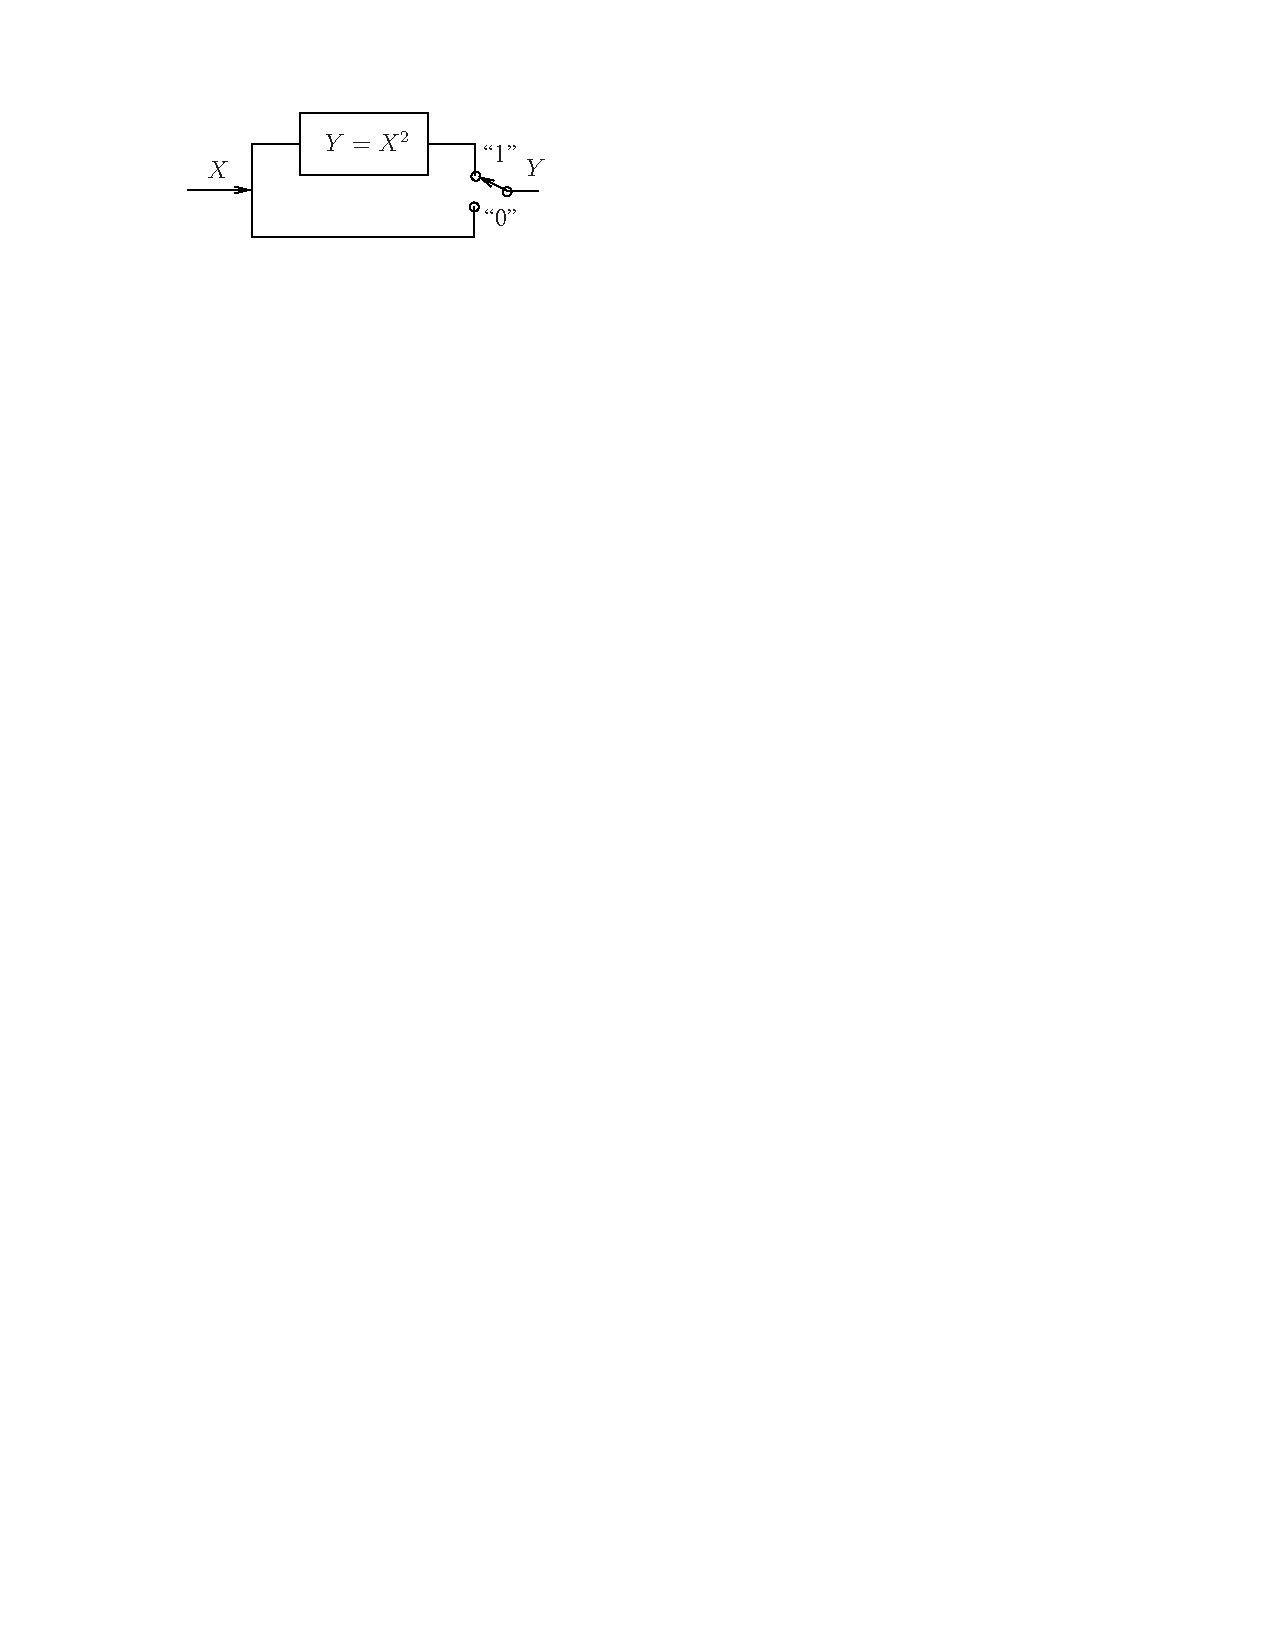
\includegraphics[width=12cm, trim=0cm 24cm 9cm 2cm]{Figuras/conmutador}
\end{center}
\end{figure}

\vspace{-0.2cm} La posici\'{o}n del conmutador no se puede observar, aunque s\'{\i} el valor de la v.a. $Y$ presente a su salida. A partir de la observaci\'{o}n de este valor, se pretende aplicar un decisor bayesiano
para decidir cu\'{a}l es la posici\'{o}n del conmutador: siendo la pol\'{\i}tica de costes $c_{00}=c_{11}=0$,
$c_{10}=2c_{01}$.
\begin{parts}
\part Form\'{u}lese el problema en la forma habitual.
\part Determ\'{\i}nese el correspondiente test, teniendo en cuenta los posibles valores de $P$. 		 
\part Calc\'{u}lense $P_{\rm FA}$ y $P_{\rm M}$.
\end{parts}
 
(Sugerencia: para determinar $p_Y(y)$, relaci\'{o}nense las funciones de distribuci\'{o}n de $Y$ y de $X$).

\begin{solution}
\begin{parts}
  \part
    $\begin{array}{ll}
 	  \displaystyle
	  H=1 : & \; Y = X^2,\; \mbox{con probabilidad} \; $P$ \\
 	  H=0 : & \; Y = X,\; \mbox{con  probabilidad} \; $1-P$ \\
	 \end{array}$
   
  \part
  	\begin{itemize}
	  \item[-] si $P>4/5: \; \Rightarrow D=1$ (siempre)
	  \item[-] si $P<4/5: \; \left\{\ \begin{array}{lll} 
	                     0<y<\dfrac{1}{16} \left(\dfrac{P}{1-P}\right)^2    & \Rightarrow & D=1 \\ \\
  	  		  	 		 \dfrac{1}{16} \left(\dfrac{P}{1-P}\right)^2 < y <1 & \Rightarrow & D=0	
  	  		  	 		 \end{array}\right.$
	\end{itemize}
	
  \part
  	\begin{itemize}
	\item[-] \vspace{0.2cm} si $P>4/5: \; P_{\rm FA} = 1; \; P_{ \rm M} = 0$
	\item[-] si $P<4/5: \; P_{\rm FA} = \dfrac{1}{16} \left(\dfrac{P}{1-P}\right)^2; \; P_{\rm M} = \dfrac{1-  \dfrac{5 P}{4}}{1-P}$
	\end{itemize}   
\end{parts}
\end{solution}

\else

\question The switch shown in the figure is in its
upper position (``1'') with known probability $P$. Random variable
$X$ has a uniform probability density $U(0,1)$.

\begin{figure}[h]
\begin{center}
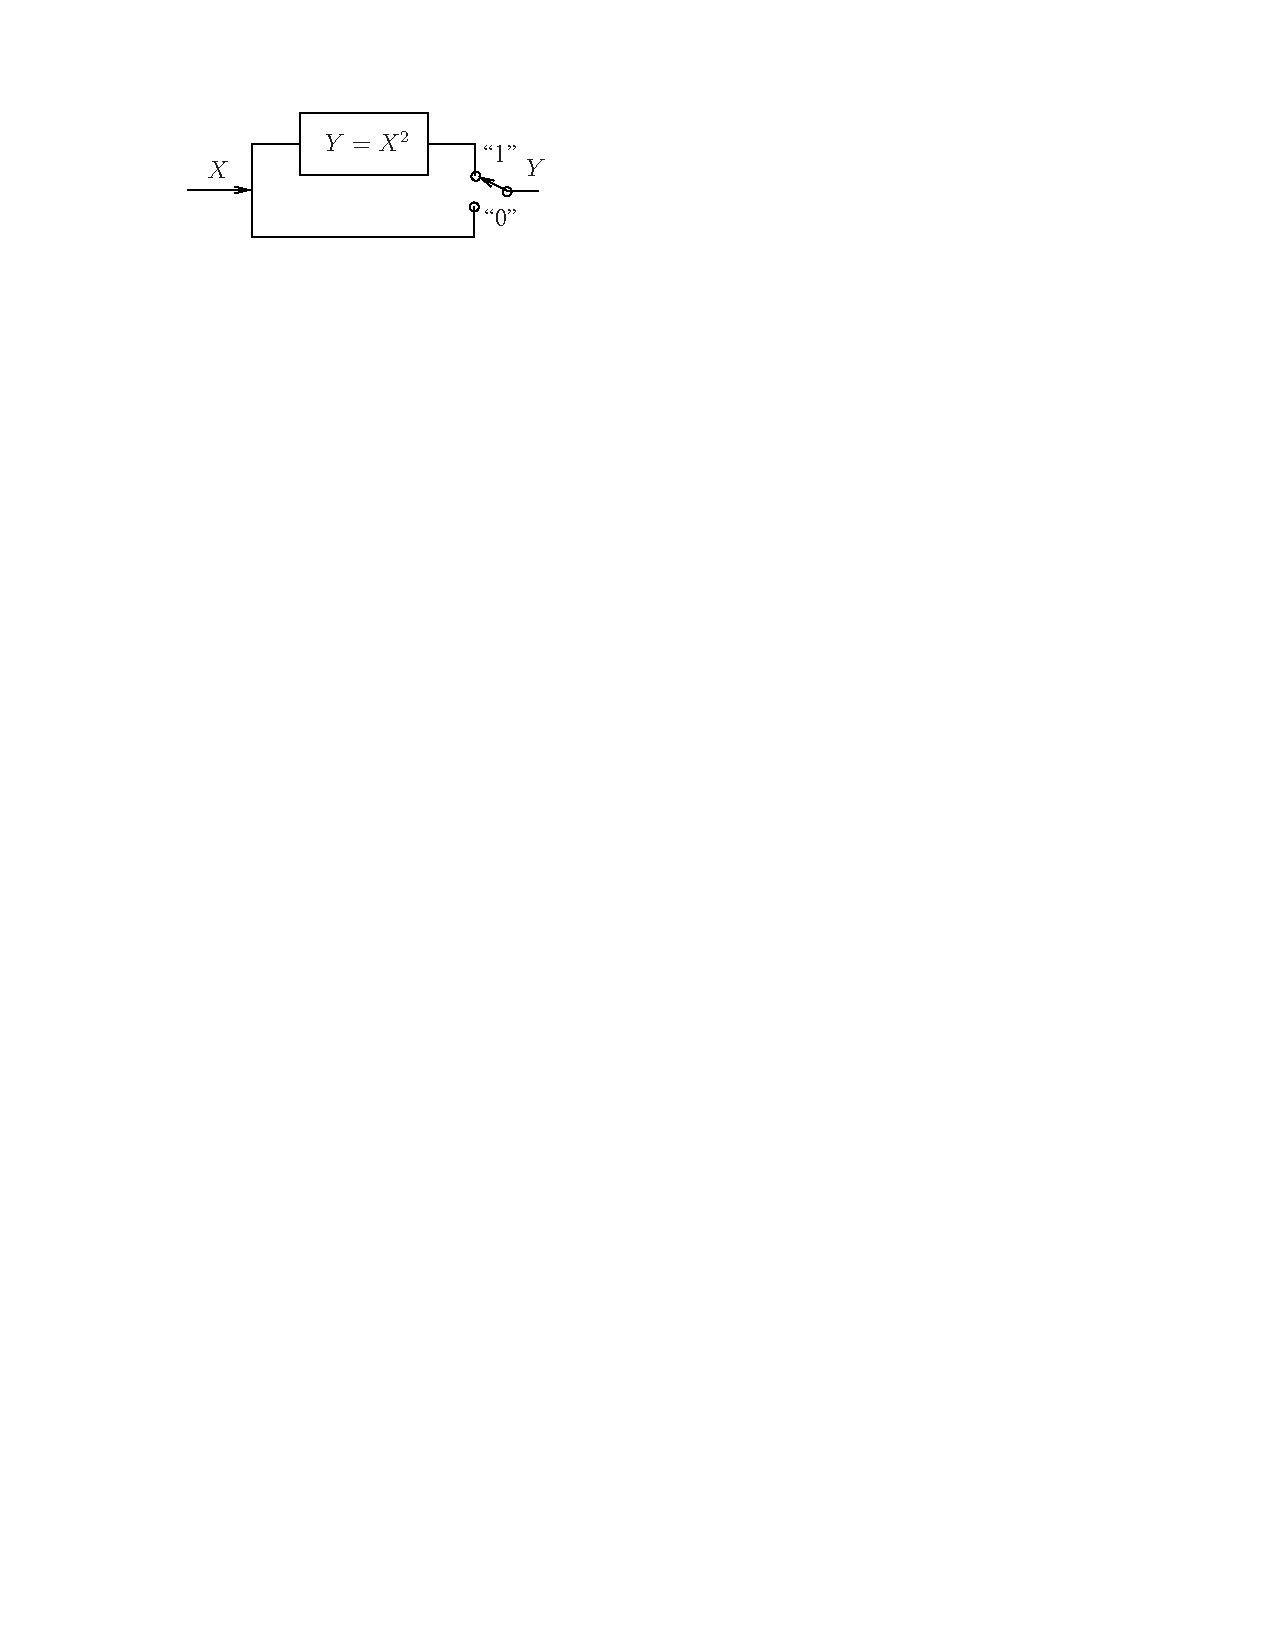
\includegraphics[width=12cm, trim=0cm 24cm 9cm 2cm]{Figuras/conmutador}
\end{center}
\end{figure}

\vspace{-0.2cm} The position of the switch cannot be observed, but the output value $Y$
is available. Based on the observation of this value, we want to apply
a Bayesian decision maker to predict which is the position of the switch.
The cost policy is $c_{00}=c_{11}=0$, $c_{10}=2c_{01}$.
\begin{parts}
 		\part Pose the problem using the usual equations for an analytical design.
 		\part Determine the corresponding test to be used, based on the possible values of $P$. 		 
 		\part Calculate $P_{\rm FA}$ and $P_{\rm M}$.
 \end{parts}
 
 (Hint: in order to find $p_Y(y)$, find the relationship that exists between the cumulative distributions of $Y$ and $X$).

\begin{solution}
	 \begin{parts}
  \part
    $
     \begin{array}{ll}
	\displaystyle
	 H=1 : & \; Y = X^2,\; \mbox{with probability} \; $P$ \\
	H=0 : & \; Y = X,\; \mbox{with probability} \; $1-P$ \\
	 \end{array} 
    $
   
  \part
  					  \begin{itemize}
					  \item[-] If $P>4/5: \; \Rightarrow D=1$ (always)
					  \item[-] If $P<4/5: \; \left\{\ \begin{array}{lll} 0<y <  \displaystyle \frac{1}{16} \left( \displaystyle \frac{P}{1-P}\right)^2 & \Rightarrow & D=1 \\ \\
					  		   	  		  	 		  \displaystyle  \frac{1}{16} \left( \displaystyle \frac{P}{1-P}\right)^2 < y <1 & \Rightarrow & D=0	\end{array}\right.$
					  \end{itemize}

  \part
  					  \begin{itemize}
					  \item[-] 	 \vspace{0.2cm} If $P>4/5: \; P_{\rm FA} = 1; \; P_{ \rm M} = 0$
					  \item[-] If $P<4/5: \; P_{\rm FA} = \displaystyle \frac{1}{16}\left( \displaystyle \frac{P}{1-P}\right)^2; \; P_{\rm M} =  \displaystyle \frac{1-  \displaystyle \frac{5 P}{4}}{1-P}$
					  \end{itemize}   
  
  
	\end{parts}
\end{solution}

\fi

%%%%%%%%%%%%%%%%%%%%%%%%%%%%%%%%%%%%%%%%%%%%%%%%%%%%%%%%%%%%%%%%%%%
\qformat{\textbf{\ej 2.E10  ~~ (2.1)} ~~ \linefill}
\ifspanish

\question Se lanza al aire un dado tradicional (caras con puntos de 1 a 6) y se genera la v.a. $X$ tal que
$$p_X(x) = \left\{\begin{array}{ll}
					\displaystyle
					\frac{2}{a} \left(1-\frac{x}{a}\right), & 0<x<a\\
					\\
					0, & {\mbox{en otro caso}}  
	 			  \end{array} 
           \right. $$
de modo tal que su media viene dada por el resultado del lanzamiento (es igual a los puntos que muestra la cara de arriba).

Sup\'{o}ngase que, para una tirada, se tiene acceso a 3 medidas del valor de $X$ tomadas independientemente, de valores $x^{(1)} = 2, x^{(2)} = 5, x^{(3)} = 10$. Dec\'{\i}dase a partir de ellas el resultado del lanzamiento del dado seg\'{u}n el criterio de m\'{a}xima verosimilitud.

\begin{solution}
El criterio de m\'{a}xima verosimilitud determina que se ha de elegir la cara 5.
\end{solution}

\else

\question A fair dice (with faces from 1 to 6) is thrown and the r.v. $X$ with pdf 
$$p_X(x) = \left\{\begin{array}{ll}
						  	\displaystyle
								  \frac{2}{a} \left(1-\frac{x}{a}\right), & 0<x<a\\
								  \\
								  0, & {\mbox{otherwise}}  
	 					 \end{array} 
						  \right.						  
				      $$
is generated so that its mean is given by the result of throwing the dice (i.e., the mean is equal to the number of points in the upper face).
Assume that for a given throw we have access to 3 independent measurements of $X$, with values $x^{(1)} = 2, x^{(2)} = 5, x^{(3)} = 10$.
Decide from these values which is the result of throwing the dice according to the maximum likelihood criterion. 


\begin{solution}
The Maximum Likelihood criterion determines that face `5' should be selected.
\end{solution}

\fi

\end{questions}

\end{document}
